% $Id$
%%%%%%%%%%%%%%%%%%%%%%%%%%%%%%%%%%%%%%%%%%%%%%%%%%%%%%%%%%%%%%%%%%%%%%

\documentclass[a4paper,11pt,oneside]{book}
\overfullrule=5pt % uncomment to mark overfull boxes
\setlength{\fboxrule}{.5mm}
\setlength{\fboxsep}{1.75mm}
\setlength{\footnotesep}{6pt}

\usepackage{amsmath}
\usepackage{amsfonts}
\usepackage{amsthm}
\usepackage{fancyvrb}
\usepackage{makeidx}
\usepackage[pdftex]{graphicx}
\usepackage{pdfpages}   % SR_2009: added new cover

\usepackage[flushmargin]{footmisc}
\usepackage{fullpage}
\usepackage[hyphens]{url} % options "hyphens" enables linebreaks in \url{}
% Literaturverzeichnis kapitelweise
\usepackage[labelstoglobalaux]{bibunits} % ohne labelstoglobalaux scheint man thebibilograpy und bibtex nicht mischen zu k�nnen
%\bibliographyunit[\section] % bibunits f�r das ganze Dokument aktivieren
\defaultbibliography{references}
\defaultbibliographystyle{abbrv}
\usepackage{float}
\usepackage{subfig}
\usepackage{shorttoc}
\usepackage[colorlinks=true,linkcolor=black,citecolor=black,urlcolor=black,bookmarksnumbered=true,pdfpagelabels,plainpages=false,hyperfootnotes=false]{hyperref}
%To reduce the number of hyperlink related 'pdfTeX warning's we use options 
%pdfpagelabels, plainpages=false and, hyperfootnotes=false and place hyperref after float.
%Option debug helps finding problems.

\floatstyle{ruled}
\newfloat{sagecode}{!ht}{loc}[chapter]
\floatname{sagecode}{Sage sample}
\newfloat{cryptoprocedure}{!ht}{lop}[chapter]
\floatname{cryptoprocedure}{Crypto Procedure}


\makeindex
\hypersetup{colorlinks=true}

% \setlength{\textwidth}{460 pt}
% \hoffset-0.7in
\newtheorem{definition}{Definition}[section]
%\newcommand{\href}[2]{#2}
\newcommand{\hypertag}[2]{#1}
%\newcommand{\hyperlink}[2]{#2}
%\newcommand{\hypertarget}[2]{#2}
\newtheorem{theorem}{Theorem}[section]
\newenvironment{Proof}[1]{\noindent\textbf{Proof #1} \\}{\hfill$\Box$\par}
\newenvironment{example}[1]{\noindent\textbf{Example#1}}{}
\newenvironment{remark}[1]{\noindent\textbf{Comment#1}}{}


% Define title %%%%%%%%%%%%%%%%%%%%%%%%%%%%%%%%%%%%%%%%%%%%%%%%%%%%%%%%%%%%%%%%%%%
\title{ % Keine Leerzeilen, sonst Meldung: "Paragraph ended before \title was complete."
	{\Huge The CrypTool Script: \\
	 \vspace{5pt}
	 Cryptography, Mathematics, and More} \\
        \vspace{20pt}
	{\LARGE	Background reading for CrypTool\\ 
         the free e-learning program\\
	 (with number theory code samples for Sage)} \\
        \vspace{15pt}
        {\large (10th edition -- distributed with CrypTool version 1.4.30)}
        \vspace{180pt}
}

% Hier wird \vspace{32pt} einfach ignoriert
\author{ % Die Klammer zur Font�nderung funktioniert bei author nur einzeilig im Gegensatz zu title?!
        {\LARGE Copyright (c) Prof.\ Bernhard Esslinger (co-author and editor)}\\
	\vspace{5pt}  % Dies wirkt sich nicht aus ???????????
        {\LARGE and the CrypTool Development Team, 1998-2010}\\
	\vspace{5pt}
        {\LARGE Frankfurt am Main, Germany} \\*[1ex]
	\vspace{5pt}
        \url{www.cryptool.org}
}


%%%%%%%%%%%%%%%%%%%%%%%%%%%%%%%%%%%%%%%%%%%%%%%%%%%%%%%%%%%%%%%%%%%%
\begin{document}
\VerbatimFootnotes

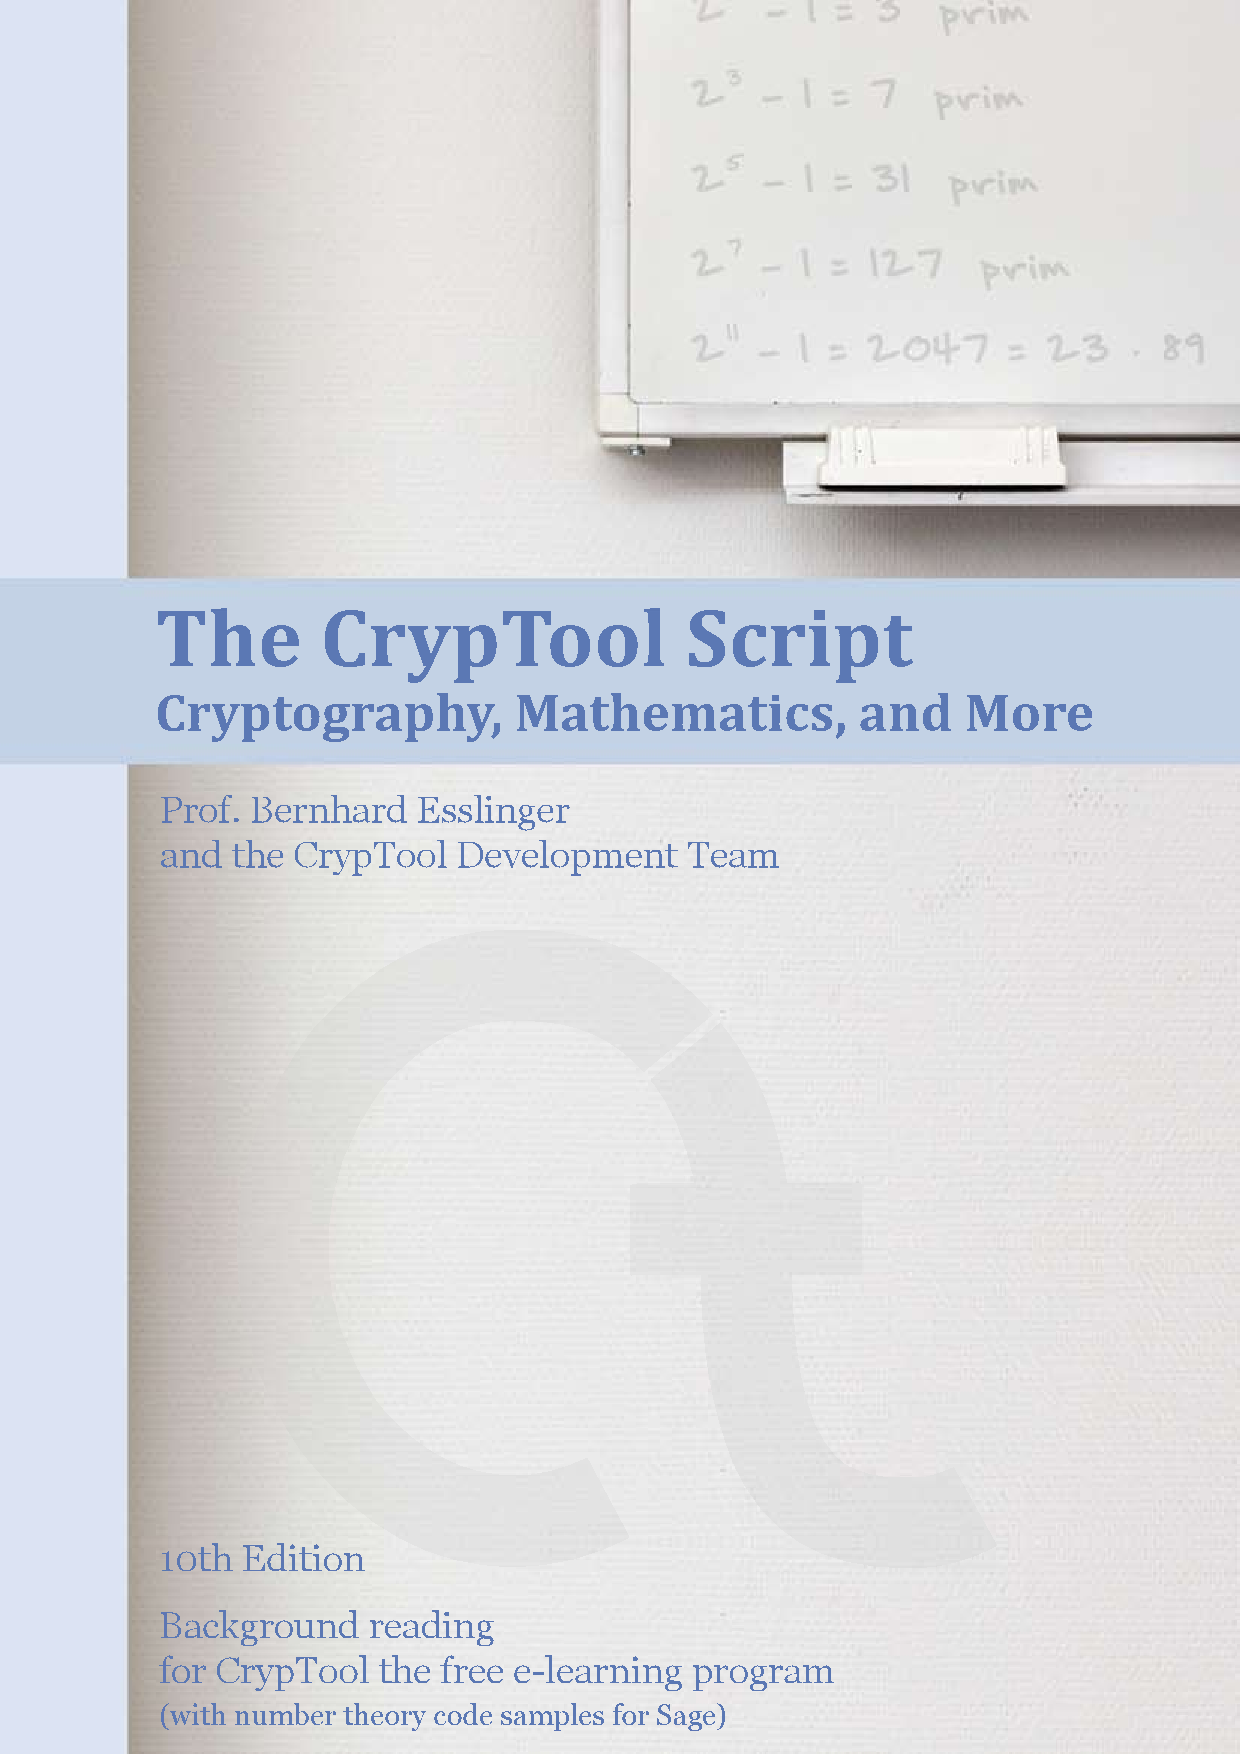
\includepdf[page=1]{figures/coverv1_en-100dpi.pdf}    % SR_2009: added new cover

\frontmatter

\pagestyle{plain}
\setlength{\fboxrule}{.5mm}
\setlength{\fboxsep}{1.75mm}
\setlength{\footnotesep}{6pt}
\addtolength{\footskip}{8pt}
%\setlength{\footskip}{4cm}
%\renewcommand{\footnoterule}{\parindent0cm\rule{13cm}{.1pt}\vspace{.2cm}}
%Formatierung der Fu"snoten

%space between text and footnote 
\renewcommand\footnoterule{%
  \vspace{2em}%   <-- one line space between text and footnoterule
%\kern-3\p@
  \hrule width .4\columnwidth
 \vspace{4pt}
%kern 2.6\p@
}

%\long\def\@makefntext#1{%
%    \parindent 1em%
%    \noindent
%    \hbox to 1.8em{\hss\@makefnmark}#1}


\maketitle


% Vergleichbar zur Nutzung von Texten aus der Wikipedia (=GNU Free Documentation Licence, GFDL)
% \vspace{200pt}
\begin{quote}
This is a free document, so the content of the document can
be copied and distributed, also for commercial purposes --- as long as
the authors, title and the CrypTool web site (\url{www.cryptool.org})
are acknowledged. Naturally, citations from the CrypTool script are
possible, as in all other documents.\\
The specific license for this document is the GNU Free Documentation Licence.

    Copyright \copyright{} 1998--2010 Bernhard Esslinger and the
    CrypTool Development Team. Permission is granted to copy,
    distribute and/or modify this document under the terms of the GNU
    Free Documentation License, Version 1.3 or any later version
    published by the Free Software Foundation; with no Invariant
    Sections, no Front-Cover Texts, and no Back-Cover Texts. A copy of
    the license is included in the section entitled
    \hyperlink{appendix-GNU-fdl}{``GNU Free Documentation License''}.
\end{quote}

\vspace{460pt}
Source cover photograph: \url{www.photocase.com}, Andre Guenther\\

Typesetting software: \LaTeX

Version control software: Subversion



% $Id$
% ............................................................................
%                 TEXT OF THE 2nd PAGE (Overview)
% ~~~~~~~~~~~~~~~~~~~~~~~~~~~~~~~~~~~~~~~~~~~~~~~~~~~~~~~~~~~~~~~~~~~~~~~~~~~~

% --------------------------------------------------------------------------
% HACK to fix warning "destination with the same identifier .. has already been used, ...":
%\makeatletter \renewcommand{\thepage}{~\csname @roman\endcsname \c@page~} \makeatother
\clearpage\phantomsection
% HACK to fix warning "destination with the same identifier .. has already been used, ...":
% \makeatletter \renewcommand{\thepage}{\csname @roman\endcsname \c@page} \makeatother

\addcontentsline{toc}{chapter}{Overview about the Content of the CrypTool Book}
\chapter*{Overview about the Content of the CrypTool Book}  

\parskip 4pt
%\vskip +12 pt
The rapid spread of the Internet has led to intensified research in the
technologies involved, especially within the area of cryptography where a good
deal of new knowledge has arisen.

In this {\em book accompanying the CrypTool programs} \index{CrypTool}
you will find predominantly mathematically oriented information on using
cryptographic procedures. Also included are many sample code pieces written in the
computer algebra system {\bf SageMath}\index{SageMath} (see appendix~\ref{s:appendix-using-sage}).
The main chapters have been written by various {\bf authors}
(see appendix~\ref{s:appendix-authors}) %\hyperlink{appendix-authors}{authors}
and are therefore independent from one another. At the end of most chapters
you will find references and web links.
The sections have been enriched with many {\em footnotes}. Within the footnotes
you can see where the described functions can be called in the different CrypTool
versions.

The \hyperlink{Kapitel_1}{first chapter} explains the principles of symmetric
and asymmetric {\bf encryption} and definitions for their resistibility.

Because of didactic reasons the \hyperlink{Kapitel_PaperandPencil}
{second chapter} gives an exhaustive overview
about {\bf paper and pencil encryption methods}.

Big parts of this book are dedicated to the fascinating topic of 
{\bf prime numbers} (chap. \ref{Label_Kapitel_Primes}).
%\hyperlink{Kapitel_2}{{\bf prime numbers}}. 
Using numerous examples, {\bf modular arithmetic} and 
{\bf elementary number theory} (chap. \ref{Chapter_ElementaryNT})
are introduced. The features of the {\bf RSA procedure} are a key aspect.

By reading chapter \ref{Chapter_ModernCryptography}
you'll gain an insight into the mathematical ideas and concepts behind 
{\bf modern cryptography}.

Chapter \ref{Chapter_Hashes-and-Digital-Signatures} gives
an overview about the status of attacks against modern {\bf hash algorithms}
and is then shortly devoted to {\bf digital signatures}, 
which are an essential component of e-business applications.

Chapter \ref{Chapter_EllipticCurves} describes {\bf elliptic curves}:
They could be used as an alternative to RSA and in addition are extremely
well suited for implementation on smartcards.

Chapter \ref{Chapter_BitCiphers} introduces {\bf Boolean algebra}.
This is the foundation for most modern symmetric encryption algorithms
as these operate on bit streams and bit groups.

Chapter \ref{Chapter_HomomorphicCiphers} describes {\bf homomorphic crypto
functions}: They are a modern research topic which got especial attention
in the course of cloud computing.

The \hyperlink{Chapter_Crypto2020}{last chapter} {\bf Crypto2020}
discusses threats for currently used cryptographic methods and introduces
alternative research approaches to achieve long-term security
of cryptographic schemes.

Whereas the CrypTool \textit{e-learning programs}\index{e-learning} motivate
and teach you how to use cryptography in practice, the \textit{book} provides
those interested in the subject with a deeper understanding of the mathematical
algorithms used -- trying to do it in an instructive way.

Within the {\bf appendices}
\ref{s:appendix-menu-overview-CT1},
\ref{s:appendix-template-overview-CT2},
\ref{s:appendix-function-overview-JCT}, and
\ref{s:appendix-function-overview-CTO}
you can gain a fast overview about the functions delivered by the different
CrypTool variants\index{CrypTool 1}\index{CrypTool 2}\index{JCrypTool} via:
\begin{itemize}
  \item the function list and
        the \hyperlink{appendix-menu-overview-CT1}
                      {menu tree of CrypTool 1 (CT1)},
  \item the function list and
        the \hyperlink{appendix-template-overview-CT2}
                      {templates in CrypTool 2 (CT2)},
  \item the \hyperlink{appendix-function-overview-JCT}
                      {function list of JCrypTool (JCT)}, and
  \item the \hyperlink{appendix-function-overview-CTO}
                      {function list of CrypTool-Online (CTO)}.
\end{itemize}

% Bernhard Esslinger, Matthias B\"uger, Bartol Filipovic, Henrik Koy, 
% Roger Oyono and J\"org Cornelius Schneider
The authors would like to take this opportunity to thank their colleagues 
in the particular companies and at the universities of Bochum, Darmstadt,
Frankfurt, Gie\ss en, Karlsruhe and Siegen.

\enlargethispage{12pt}
As with the e-learning program CrypTool\index{CrypTool}, the quality of the 
book is enhanced by your suggestions and ideas for improvement. 
We look forward to your feedback.


% Local Variables:
% TeX-master: "../script-en.tex"
% End:


\newpage
\pdfbookmark[0]{Contents Overview}{ShortContents}
\shorttoc{Contents Overview}{0}
\clearpage\phantomsection
\pdfbookmark[0]{\contentsname}{Contents}
\tableofcontents 

\newpage
\normalsize

%\parindent 0cm

% \parskip 4pt
% Setting the default for the vertical distance before a paragraph as distinguished variable
\newcounter{mycounterDefaultParskip}
\setcounter{mycounterDefaultParskip}{4}
\parskip \value{mycounterDefaultParskip} pt 


% $Id$
% ............................................................................
%      V O R W O R T  und  E I N F � H R U N G (Zusammenspiel Skript-CT) 
% ~~~~~~~~~~~~~~~~~~~~~~~~~~~~~~~~~~~~~~~~~~~~~~~~~~~~~~~~~~~~~~~~~~~~~~~~~~~~


% --------------------------------------------------------------------------
\clearpage\phantomsection
\addcontentsline{toc}{chapter}{Preface to the 10th Edition of the CrypTool Script}
\chapter*{Preface to the 10th Edition of the CrypTool Script}

Starting in the year 2000 this script became part of the 
CrypTool v1\index{CrypTool 1.x} package. It is designed to accompany the program 
CrypTool by explaining some mathematical topics in more detail, 
but still in a way which is easy to understand.

In order to also enable developers/authors to work together independently 
the topics have been split up and for each topic an extra chapter has been 
written which can be read on its own. The later editorial work in TeX added 
cross linkages between different sections and footnotes describing where you
can find the according functions within the CrypTool v1\index{CrypTool 1.x} 
program \hyperlink{appendix-menutree}{(see menu tree} in appendix \ref{s:appendix-menutree}).
% \hypertarget{appendix-menutree}{}\label{s:appendix-menutree}
Naturally there are many more interesting topics in mathematics and
cryptography which could be discussed in greater depth -- therefore this
is only one of many ways to do it.

The rapid spread of the Internet has also lead to intensified research in the
technologies involved, especially within the area of cryptography where a good
deal of new knowledge has arisen.

%This edition of the script adds some topics, but mainly updates areas (e.g. the
%summaries of topical research areas):
This edition completely updated the TeX sources of the document, and of course
the content of the script was corrected, amended and updated with some topics, e.g.:
\vspace{-7pt}
\begin{itemize}
  \item the search for the largest prime numbers 
        (chap. \ref{search_for_very_big_primes}), 
  \item progress in cryptanalysis of hash algorithms 
        (chap. \ref{NeueAES-Analyse}) and
%  \item progress in cryptanalysis of hash algorithms 
%        (chap. \ref{collision-attacks-against-sha-1}) and
%  \item progress in ideas for new crypto methods (RSA successor) 
%        (chap. \ref{xxxxxxxxxBrute-force-gegen-Symmetr})\index{xxxxxxxxxxxxxxxx} and
  \item the list of movies or novels, in which cryptography or number theory 
        played major role (see appendix \ref{s:appendix-movies});
        and where primes are used as hangers  
        (see curiouses in \ref{HT-Quaint-curious-Primes-usage}).
\end{itemize}

Newly added is the appendix \ref{s:appendix-using-sage} about using the
computer algebra system Sage. This was added because Sage becomes
more and more the standard open-source CAS system. Accordingly all
samples written before in Pari-GP and Mathematica have been substituted
with Sage code. Thanks to Minh Van Nguyen, a lot of new code samples could be added.

The first time the document was delivered with CrypTool\index{CrypTool} 
was in version 1.2.01. Since then it has been expanded and revised in almost
every new version of CrypTool.

I am deeply grateful to all the people helping with their impressive
commitment who have made this global project so successful.
Thanks also to the readers who sent us feedback.
% Especially I would like to acknowledge the English language proof-reading
% of this script version done by Richard Christensen and Lowell Montgomery.

I hope that many readers have fun with this script and that they get 
out of it more interest and greater understanding of this modern but 
also very ancient topic.
\\
\\
% [1.5\baselineskip]
% \enlargethispage*{2\baselineskip}
% \nopagebreak
Bernhard Esslinger
\\
\\
% [\baselineskip]
Frankfurt (Germany), August 2009



% --------------------------------------------------------------------------
\clearpage\phantomsection
\addcontentsline{toc}{chapter}{Introduction -- How do the Script and the Program Play together?}
\chapter*{Introduction -- How do the Script and the Program Play together?}

\textbf{This script}

This document is delivered together with the open-source program CrypTool\index{CrypTool}.

The articles in this script are largely self-contained and
can also be read independently of CrypTool\index{CrypTool}.

Chapters  \ref{Chapter_ModernCryptography} (Modern Cryptography) and 
\ref{Chapter_EllipticCurves} (Elliptic Curves) require a deeper knowledge
in mathematics, while the other chapters should be understandable with a 
school leaving certificate.

The \hyperlink{appendix-authors}{authors}
have attempted to describe cryptography for a broad 
audience -- without being mathematically incorrect. We believe that this
didactic pretension is the best way to promote the awareness for IT
security and the readiness to use standardized modern cryptography.
\par \vskip + 15pt


\noindent \textbf{The program CrypTool\index{CrypTool}}

CrypTool\index{CrypTool} is an educational program with a comprehensive online
help enabling you to use and analyse cryptographic procedures within a
unified graphical user interface.

CrypTool\index{CrypTool} is used world-wide for 
training in companies and teaching at schools and universities worldwide, and
several universities are helping to further develop the project.
\par \vskip + 15pt


\noindent \textbf{Acknowledgment}

At this point I'd like to thank explicitly the following people who
particularly contributed to CrypTool\index{CrypTool}. They applied their
very special talents and showed really great engagement:
\vspace{-7pt}
%\begin{itemize}
\begin{list}{\textbullet}{\addtolength{\itemsep}{-0.5\baselineskip}}
   \item Mr.\ Henrik Koy
   \item Mr.\ J\"org-Cornelius Schneider
   \item Mr.\ Florian Marchal
   \item Dr.\ Peer Wichmann
   \item Staff of Prof.\ Claudia Eckert, Prof.\ Johannes Buchmann and Prof.\ Torben Weis.
\end{list}
%\end{itemize}
Also I want to thank all the many people not mentioned here for their 
hard work (mostly carried out in their spare time).
\\
\\
Bernhard Esslinger
\\
\\
Frankfurt (Germany), July 2009

% Local Variables:
% TeX-master: "../script-en.tex"
% End:


\mainmatter

% ..............................................................................
%                V E R S C H L U E S S E L U N G S V E R F A H R E N
% ~~~~~~~~~~~~~~~~~~~~~~~~~~~~~~~~~~~~~~~~~~~~~~~~~~~~~~~~~~~~~~~~~~~~~~~~~~~~~~

\newpage
\section{Encryption procedures}
\hypertarget{Kapitel_1}{}
(Bernhard Esslinger, besslinger@web.de, May 1999, Updates Dec. 2001, Feb. 2003)


% --------------------------------------------------------------------------
\subsection{Encryption}

The purpose of encryption \index{Encryption} is to change data in such a way
that only an authorised recipient is able to reconstruct the plaintext. This has
the advantage that you can transmit encrypted data openly and nevertheless need
not fear a perpetrator reading the data without authorisation. Authorised
recipients possess a piece of secret information --- called the key --- which
allows them to decrypt the data while it remains hidden from everyone else.\par \vskip + 3pt

One encryption procedure has been proved to be secure --- the {\em One Time
  Pad}.
\index{One �Time �Pad} However, this procedure has several practical
disadvantages (the key used must be selected randomly and must be just as long
as the message to be protected), which means that it is hardly used except in
closed environments such as for the hot wire between Moscow and Washington.\par \vskip + 3pt

For all other procedures there is a (theoretical) possibility of breaking them.
If the procedures are good, however, the time taken to break them is so long
that it is practically impossible to do and these procedures can therefore be
considered (practically) secure.\par \vskip + 3pt

We basically distinguish between symmetric and asymmetric encryption procedures.

% --------------------------------------------------------------------------
\subsubsection[Symmetric encryption]
{Symmetric encryption\footnotemark}
\footnotetext{%
With CrypTool\index{CrypTool} v1.3 you can execute the following modern
symmetric encryption algorithms 
(using the menu ``Crypt \textbackslash Symmetric''): \\
IDEA, RC2, RC4, DES (ECB), DES�(CBC), Triple-DES�(ECB), Triple-DES�(CBC),
MARS (AES candidate), RC6 (AES candidate), Serpent (AES candidate), 
Twofish (AES candidate), Rijndael (official AES algorithm).
}

For {\em symmetric} encryption \index{Encryption!symmetric} the sender and
recipient must possess a common (secret) key which they have exchanged before
actually starting to communicate. The sender uses this key to encrypt the
message and the recipient uses it to decrypt it.\par \vskip + 3pt

The advantages of symmetric algorithms are the high speed with which data can be
encrypted and decrypted. One disadvantage is the need for key management. In
order to communicate with one another confidentially, sender and recipient must
have exchanged a key using a secure channel before actually starting to
communicate. Spontaneous communication between individuals who have never met
therefore seems virtually impossible. If everyone wants to communicate with
everyone else spontaneously at any time in a network of $ n $ subscribers, each
subscriber must have previously exchanged a key with each of the other $n-� 1$
subscribers. A total of $n(n - 1)/2$ keys must therefore be exchanged.\par \vskip + 3pt

The most well-known symmetric encryption procedure is the \index{DES} DES-algorithm. The DES-algorithm has been developed by IBM in collaboration with the
National Security Agency \index{NSA} (NSA), and was published as a standard in
1975. Despite the fact that the procedure is relatively old, no effective attack
on it has yet been detected. The most effective way of attacking consists of
testing all possible keys until the right one is found ({\em brute-force-attack}).
\index{Attack!brute-force} Due to the relatively short key length of
effectively 56 bits (64 bits, which however include 8 parity bits), numerous
messages encrypted using DES have in the past been broken. Therefore, the
procedure can now only be considered to be conditionally secure. Symmetric
alternatives to the DES procedure include the IDEA \index{IDEA} or Triple DES
algorithms.\par \vskip + 3pt

Up-to-the-minute procedures are the symmetric AES procedures. The associated
Rijndael procedure was declared winner the AES award on 2 October 2000 and thus
succeeds the DES procedure.

More details about the AES algorithms can be found within the Online help of CrypTool\index{CrypTool} (in the index see head-word {\em AES} and then the help pages {\em AES candidates}, {\em The AES Winner Rijndael} and {\em The Rijndael encryption algorithm}).


% --------------------------------------------------------------------------
\subsubsection{New results about cryptanalysis of AES}

Below you will find some results, which have recently called into question the security of the AES algorithm -- from our point of view these doubts practically still remain unfounded. The following information is based on the original papers and the articles \cite{Wobst-iX2002} and \cite{Lucks-DuD2002}.

AES with a minimum key length of 128 bit is still in the long run sufficiently secure against brute-force attacks - as long as the quantum computers weren't powerful enough. When announced as new standard AES was immune against all known crypto attacks, mostly based on statistical considerations and earlier applied to DES: using pairs of clear and cipher texts expressions are constructed, which are not completely at random, so they allow conclusions to the used keys. These attacks required unrealistically large amounts of intercepted data.

Cryptanalysts already label methods as ``academic success'' or as ``cryptanalytic attack'' if they are theoretically faster than the complete testing of all keys (brute force analysis). In the case of AES with the maximal key length (256 bit) exhaustive key search on average needs $2^{255}$ encryption operations. A cryptanalytic attack needs to be better than this. At present between $2^{75}$ and $2^{90}$ encryption operations are estimated to be performable for organizations, for example a security agency.

In their 2001-paper Ferguson, Schroeppel and Whiting \cite{Ferguson2001} presented a new method of symmetric codes cryptanalysis: They described AES with a closed formula (in the form of a continued fraction) which was possible because of the "relatively" clear structure of AES. This formula consists of around 1000 trillion terms of a sum - so it does not help concrete practical cryptanalysis. Nevertheless -curiosity in the academic community awakened. It was already known, that the 128-bit AES could be described as an over-determined system of about 8000 quadratic equations (over an algebraic number field) with about 1600 variables (some of them are the bits of the wanted key) -- equation systems of that size are in practice not solvable. This special equation system is relatively sparse, so only very few of the quadratic terms (there are about 1,280,000 are possible quadratic terms in total) appear in the equation system.

The mathematicians Courois and Pieprzyk \cite{Courtois2002} published a paper in 2002, which got a great deal of attention amongst the crypto community: The pair had further developed the XL-method (eXtended Linearization), introduced at Eurocrypt 2000 by Shamir et al., to create the so called XSL-method (eXtended Sparse Linearization). The XL-method is a heuristic technique, which in some cases manages to solve big non-linear equation systems and which was till then used to analyze an asymmetric algorithm (HFE).  The innovation of Courois and Pieprzyk was, to apply the XL-method on symmetric codes: the XSL-method can be applied to very specific equation systems. A 256-bit AES could be attacked in roughly $2^{230}$ steps. This is still a purely academic attack, but also a direction pointer for a complete class of block ciphers. The major problem with this attack is that until now nobody has worked out, under what conditions it is successful: the authors specify in their paper necessary conditions, but it is not known, which conditions are sufficient.
There are two very new aspects of this attack: firstly this attack is not based on statistics but on algebra. So attacks seem to be possible, where only very small amounts of cipher text are available. Secondly the security of a product-algorithm does not exponentially increase with the number of rounds.

Currently there is a large amount of research in this area: for example Murphy and Robshaw presented a paper at Crypto 2002 \cite{Robshaw2002a}, which could dramatically improve cryptanalysis: the burden for a 128-bit key was estimated at about $2^{100}$ steps by describing AES as a special case of an algorithm called BES (Big Encryption System), which has an especially "round" structure. But even $2^{100}$ steps are beyond what is achievable in the foreseeable future. Using a 256 bit key the authors estimate that a XSL-attack will require $2^{200}$ operations.

More details can be found at: \\
\href{http://www.cryptosystem.net/aes}{\texttt{http://www.cryptosystem.net/aes}} and \\ 
\href{http://www.minrank.org/aes/}{\texttt{http://www.minrank.org/aes/}}

So for 256-AES the attack is much more effective than brute-force but still far away from any computing power which could be accessible in the short-to-long term. The discussion is very controversial: Don Coppersmith (one of the inventors of DES) for example queries the practicability of the attack because XLS would provide no solution for AES \cite{Coppersmith2002}. This concludes that then the optimization of Murphy and Robshaw \cite{Robshaw2002b} would not work.


% --------------------------------------------------------------------------
\subsubsection{Asymmetric encryption}

In the case of {\em asymmetric} encryption \index{Encryption!asymmetric} each
subscriber has a personal pair of keys consisting of a {\em secret}
\index{Key!secret} key and a {\em public} key\index{Key!public}. The public
key, as its name implies, is made public, e.g. in a key directory on the
Internet.\par \vskip + 3pt

If Alice wants to communicate with Bob, then she finds Bob's public key 
in the directory and uses it to encrypt her message to him. She then sends
this cipher text to Bob, who is then able to decrypt it again using his 
secret key. As only Bob knows his secret key, only he can decrypt 
messages addressed to him.
Even Alice who sends the message cannot restore plaintext from the (encrypted)
message she has sent. Of course, you must first ensure that the public key
cannot be used to derive the private key.\par \vskip + 3pt

Such a procedure can be demonstrated using a series of thief-proof letter boxes.
If I have composed a message, I then look for the letter box of the recipient
and post the letter through it. After that, I can no longer read or change the
message myself, because only the legitimate recipient possesses the key for the
letter box.\par \vskip + 3pt

The advantage of asymmetric procedures is the easy \index{Key management} key management. Let's look again at a network with $n$
subscribers. In order to ensure that each subscriber can establish
an encrypted connection to each other subscriber, each subscriber
must possess a pair of keys. We therefore need $2n$ keys or $n$
pairs of keys. Furthermore, no secure channel is needed before
messages are transmitted, because all the information required in
order to communicate confidentially can be transmitted openly. In
this case, you simply have to pay attention to the accuracy
(integrity and authenticity) \index{Authenticity} of the public
key. Disadvantage: Pure asymmetric procedures take a lot longer to
perform than symmetric ones.\par \vskip + 3pt

The most well-known asymmetric procedure is the \index{RSA} RSA algorithm,
named after its developers Ronald \index{Rivest Ronald} Rivest, Adi
\index{Shamir Adi} Shamir and Leonard \index{Adleman Leonard} Adleman. The RSA algorithm
was published in 1978. The concept of asymmetric encryption was first
introduced by Whitfield Diffie \index{Diffie Whitfield}  and Martin
\index{Hellman Martin} Hellman in 1976. Today, the ElGamal \index{ElGamal}
procedures also play a decisive role, particularly the \index{Schnorr} Schnorr
variant in the \index{DSA} DSA (Digital \index{Signatures!digital}Signature
Algorithm).


% --------------------------------------------------------------------------
\newpage
\subsubsection[Hybrid procedures]
{Hybrid procedures\footnotemark}
\footnotetext{%
Within CrypTool\index{CrypTool} v1.3 you can get a visualization of this
technique using the menu ``Crypt \textbackslash Hybrid Demonstration'': 
this dialogue shows the single steps and its dependencies with concrete
numbers.
}\index{Hybrid procedures}

In order to benefit from the advantages of symmetric and asymmetric techniques
together, hybrid procedures are usually used (for encryption) in practice.
\par \vskip + 3pt

In this case the data is encrypted using symmetric procedures: the key is a
session key\index{Session key} generated by the sender randomly that is only used for this message.
This session key is then encrypted using the asymmetric procedure and
transmitted to the recipient together with the message. Recipients can determine
the session key using their secret keys and then use the session key to encrypt
the message. In this way, we can benefit from the easy key management
\index{Key management} of asymmetric procedures and encrypt large quantities of data
quickly and efficiently using symmetric procedures.


% --------------------------------------------------------------------------
\subsubsection{Further details}

Beside information you can find in many books and on a lot of websites the 
online help of CrypTool\index{CrypTool} also offers very many details about
the symmetric and asymmetric encryption methods.


% --------------------------------------------------------------------------
\begin{thebibliography}{99999}
\addcontentsline{toc}{subsection}{Bibliography}

\bibitem[Schmeh2003]{Schmeh2003}  \index{Schmeh 2003}
        Klaus Schmeh, \\
        {\em Cryptography and Public Key Infrastructures on the Internet}, 
	John Wiley \& Sons Ltd., Chichester 2003. \\
        A considerable, up-to-date, good reading book, which also 
	considers practical problems, like standardisation or
        real existing software.


\bibitem[Coppersmith2002]{Coppersmith2002}  \index{Coppersmith 2002}
        Don Coppersmith, \\
        {\em Re: Impact of Courtois and Pieprzyk results}, 
	2002-09-19, AES Discussion Groups at \\
        \href{http://aes.nist.gov/aes/}
        {\texttt{http://aes.nist.gov/aes/}}

\bibitem[Courtois2002]{Courtois2002}  \index{Courtois 2002}
        Nicolas Courtois, Josef Pieprzyk, \\
        {\em Cryptanalysis of Block Ciphers with Overdefined Systems of Equations}, 
	received 10 Apr 2002, last revised 9 Nov 2002,
	A different version, so called compact version of the first XSL attack,
	was published in Asiacrypt Dec 2002, \\
        \href{http://eprint.iacr.org/2002/044}
        {\texttt{http://eprint.iacr.org/2002/044}}

\bibitem[Ferguson2001]{Ferguson2001}  \index{Ferguson 2001}
        Niels Ferguson, Richard Schroeppel, Doug Whiting, \\
        {\em A simple algebraic representation of Rijndael}, 
	Draft 2001/05/1, \\
        \href{http://www.xs4all.nl/~vorpal/pubs/rdalgeq.html}
        {\texttt{http://www.xs4all.nl/\~{}vorpal/pubs/rdalgeq.html}}

\bibitem[Lucks-DuD2002]{Lucks-DuD2002}  \index{Lucks 2002}
        Stefan Lucks, R"udiger Weis, \\
        {\em Neue Ergebnisse zur Sicherheit des Verschl�sselungsstandards AES}, 
	in DuD Dec. 2002.

\bibitem[Robshaw2002a]{Robshaw2002a}  \index{Robshaw 2002}
        S.P. Murphy, M.J.B. Robshaw, \\
        {\em Essential Algebraic Structure within the AES}, 
	June 5, 2002, Crypto 2002,  \\
        \href{http://www.isg.rhul.ac.uk/\~{}mrobshaw/rijndael/rijndael.html}
        {\texttt{http://www.isg.rhul.ac.uk/~mrobshaw/rijndael/rijndael.html}}

\bibitem[Robshaw2002b]{Robshaw2002b}  \index{Robshaw 2002}
        S.P. Murphy, M.J.B. Robshaw, \\
        {\em Comments on the Security of the AES and the XSL Technique}, 
	September 26, 2002, \\
        \href{http://www.isg.rhul.ac.uk/\~{}mrobshaw/rijndael/rijndael.html}
        {\texttt{http://www.isg.rhul.ac.uk/~mrobshaw/rijndael/rijndael.html}}

\bibitem[Wobst-iX2002]{Wobst-iX2002}  \index{Wobst 2002}
        Reinhard Wobst, \\
        {\em Angekratzt - Kryptoanalyse von AES schreitet voran}, 
	in iX Dec. 2002, \\
	plus the reader's remark by Johannes Merkle in iX Feb. 2003.

\end{thebibliography}


% Local Variables:
% TeX-master: "../script-en.tex"
% End:

% $Id$
% ..............................................................................
%                V E R S C H L U E S S E L U N G S V E R F A H R E N
%
% Writing rule: Capitel header with all nouns/verbs-words capitalized,
%               All other headers in the normal lower/upper case manner
%               like sentences (without a dot at the end).
% Writing rule: Use American English instead of British English consistently.
%
% ~~~~~~~~~~~~~~~~~~~~~~~~~~~~~~~~~~~~~~~~~~~~~~~~~~~~~~~~~~~~~~~~~~~~~~~~~~~~~~
%------------------------------------------------------------------------------
% First Editor: Christine St�tzel, April 2004
% Update and corrections: B. Esslinger, June 2005
% Update and corrections: B. Esslinger, June 2005
% Update B. Esslinger and Minh Van Nguyen, July 2009 
%------------------------------------------------------------------------------

% ``primenet''
\newpage
\hypertarget{Kapitel_PaperandPencil}{}

\chapter{Paper and Pencil Encryption Methods}
\label{Kapitel_PaperandPencil}
(Christine St\"otzel, April 2004; Updates: B.+C. Esslinger, June 2005; Updates Minh Van Nguyen and B. Esslinger, July 2009)
\index{Paper and pencil methods}

\begin{center}
\fbox{\parbox{15cm}{%
{\em Edgar Allan Poe\index{Poe, Edgar Allan}: 
A Few Words on Secret Writing, 1841}\\
Few persons can be made to believe that it is not quite an easy thing
to invent a method of secret writing which shall baffle investigation.
Yet it may be roundly asserted that human ingenuity cannot concoct a
cipher which human ingenuity cannot resolve.}}
\end{center}

The following chapter provides a broad overview of paper and pencil 
methods\footnote{%
The footnotes to this chapter describe how the methods can be
performed using CrypTool CrypTool 1.
Additionally the last sub chapter (\ref{PaP_Sage_samples})
contains example code using the computer algebra system Sage\index{Sage}.
                 }
each with references to deeper information.
All techniques that people can apply manually to en- and decipher a message are 
embraced by this term. These methods were and still are especially popular with
secret services, as a writing pad and a pencil -- in contrast to electronic
aids -- are totally unsuspicious.

The first paper and pencil methods already arose about 3000 years ago, but new
procedures were developed during the past century, too. All paper and pencil 
methods are a matter of symmetric methods\index{Encryption!symmetric}. 
Even the earliest encryption algorithms use the basic principles such as 
transposition, substitution, block construction and their combinations. 
Hence it is worthwhile to closely consider this ``ancient'' methods especially
under didactic aspects.

Methods to be successful and wide-spread had to fulfill some attributes which are equally required for modern algorithms:
\begin{itemize}
\item Exhaustive description, almost standardization (including special cases,
      padding, etc.).
\item Good balance between security and usability 
      (because methods being too complicated were error-prone or
      unacceptably slow).
\end{itemize}


\newpage
%------------------------------------------------------------------------------
\section{Transposition ciphers}
\label{PaP_transposition_ciphers}
\index{Transposition}

Encrypting a message by means of transposition\index{Transposition} does not 
change the original characters of this message, only their order is modified
(transposition = exchange)\footnote{Another name used for transposition is
permutation\index{Permutation}.}.

%------------------------------------------------------------------------------
\subsection{Introductory samples of different transposition ciphers}
\label{introsamplesTranspositionCiphers}

\begin{itemize}

\item {\bf Rail Fence}\footnote{%
   This method can directly be found in CrypTool\index{CrypTool} at the menu item
   {\bf Crypt/Decrypt \textbackslash{} Symmetric (classic) \textbackslash{} Scytale / Rail Fence}.
   You can simulate this method also under the menu {\bf Crypt/Decrypt \textbackslash{} 
   Symmetric (classic) \textbackslash{} Permutation}: For a Rail Fence with
   2 lines use as key ``B,A'' and accept the default settings (only one
   permutation, where your input is done line-by-line and the output is
   taken column-by-column). 
   Using the key ``A,B'' would start the zigzag pattern below in the
   way, that the first letter is written into the first line instead of the
   second line.}
   \cite{pp:Singh2001}\index{Rail Fence cipher}:
   The characters of a message are alternately written in two (or more) lines,
   creating a zigzag pattern. The resulting ciphertext is read out 
   line by line.\\
   This is more a children's method.

   Plaintext\footnote{If the alphabet only uses 26 letters, we write the
   plaintext in small letters and the ciphertext in capital letters.}%
   : an example of transposition

\begin{table}[ht]
\begin{center}
\begin{tabular}{r@{\:}r@{\:}r@{\:}r@{\:}r@{\:}r@{\:}r@{\:}r@{\:}r@{\:}r@{\:}r@{\:}r@{\:}r@{\:}r@{\:}r@{\:}r@{\:}r@{\:}r@{\:}r@{\:}r@{\:}r@{\:}r@{\:}r@{\:}r@{\:}}
	  & n &   & x &   & m &   & l &   & o &   & t &   & a &   & s &   & o &   & i &   & i &   & n \\
	a &   & e &   & a &   & p &   & e &   & f &   & r &   & n &   & p &   & s &   & t &   & o &   \\
\end{tabular}
\caption{Rail Fence cipher}
\end{center} 
\end{table}

   Ciphertext\footnote{The letters of the cleartext are -- as used 
   historically -- grouped within blocks of 5 letters. It does not matter
   if the (constant) block length is different or no blank is inserted.}%
   : NXMLO TASOI INAEA PEFRN PSTO\\


\item {\bf Scytale}\footnote{%
   This method can directly be found in CrypTool\index{CrypTool} at the menu item
   {\bf Crypt/Decrypt \textbackslash{} Symmetric (classic) \textbackslash{} Scytale / Rail Fence}.
   As this method is a special case of a simple columnar transposition, you also can
   simulate it in CrypTool\index{CrypTool} under the 
   menu {\bf Crypt/Decrypt \textbackslash{} Symmetric (classic) \textbackslash{} 
   Permutation}: For the Scytale within the dialog box only the first 
   permutation is used. If the wood has e.g. 4 angles use as key ``1,2,3,4''.
   This is equivalent to write the text horizontally in blocks of 4 letters 
   in a matrix and to read it out vertically . 
   Because the key is in an in ascending order, the Scytale is denoted as
   an identical permutation. And because writing and read-out is done only
   once it is a simple (and no double) permutation.}
   \cite{pp:Singh2001}\index{Scytale}%
   : 
   This method was probably used since 600 B.C. -- a description
   of how it operated is not known from before Plutarch (50-120 B.C.).\\
   A long strip of paper is wrapped around a wooden cylinder and then the 
   message is written along the length of this strip. The ciphertext is 
   produced by unwinding the strip.

\item {\bf Grille} \cite{pp:Goebel2003}: Both parties use identical stencils. 
   Line by line, their holes are filled with plaintext that is read out 
   column by column to produce the ciphertext. If there is plaintext left, 
   the procedure is repeated\footnote{%
   This method cannot be simulated with a pure column transposition.}.

   \hypertarget{turning-grille}{}
\item {\bf Turning grille} \cite{pp:Savard1999}%
   \index{Turning grille}: 
   The German army used turning 
   grilles during WW1\footnote{The turning grille was already invented in 
   1881 by Eduard Fleissner von Wostrowitz.\\
   A good visualization can be found under www.turning-grille.com.}%
   . 
   A square grille serves as a stencil, a quarter of its fields being holes.
   The first part of the message is written on a piece of paper through	these
   holes, then the grille is rotated by 90 degrees and the user can
   write down the second part of the message, etc. But this method does only
   work, if the holes are chosen carefully: Every field has to be used, and
   no field may be used twice, either. The ciphertext is read out line by
   line.

   In the example for a turning grille in the following table you can write
   4 times 16 characters of the cleartext on a piece of paper:
\begin{table}[ht]
\begin{center}
\begin{tabular}{|cccc|cccc|}
\hline 	
	O & - & - & - & - & O & - & - \\
	- & - & - & O & O & - & - & O \\
	- & - & - & O & - & - & O & - \\
	- & - & O & - & - & - & - & - \\
\hline 	
	- & - & - & - & O & - & - & - \\
	O & - & O & - & - & - & O & - \\
	- & O & - & - & - & - & - & O \\
	- & - & - & O & O & - & - & - \\
\hline
\end{tabular}  
\caption{8x8 turning grille} 
\end{center}   
\end{table}

\end{itemize}


%------------------------------------------------------------------------------
% {\bf Column and row transposition}
\subsection[Column and row transposition ciphers]
    {Column and row transposition\footnotemark}
    \footnotetext{%
Most of the following methods can be simulated in CrypTool\index{CrypTool} 
under the menu {\bf Crypt/Decrypt \textbackslash{} Symmetric (classic) 
\textbackslash{} Permutation}.}

\begin{itemize}

\item {\bf Simple columnar transposition} \cite{pp:Savard1999}: First of all, 
   a keyword is chosen, that is written above the columns of a table. This
   table is filled with the text to be encrypted line by line. Then the 
   columns are rearranged by sorting the letters of the keyword alphabetically.
   Afterwards the columns are read out from left to right to build the 
   ciphertext\footnote{%
   Using CrypTool: Choose a key for the 1st permutation, input line by line, 
   permute and output column by column.}.

   Plaintext: an example of transposition

\begin{table}[ht]
\begin{center}
\begin{tabular}{|c|c|c|}
\hline 	
	K & E & Y \\
\hline
	a & n & e \\
	x & a & m \\
	p & l & e \\
	o & f & t \\
	r & a & n \\
	s & p & o \\
	s & i & t \\
	i & o & n \\
\hline
\end{tabular}
\caption{Simple columnar transposition}
\end{center} 
\end{table}

   Transposition key: K=2; E=1; Y=3. \\
   Ciphertext: NALFA PIOAX PORSS IEMET NOTN\\

\item {\bf AMSCO} \cite{pp:ACA2002}\index{AMSCO}: The characters of the plaintext
   are written in alternating groups of one respectively two letters into a
   grille. Then the columns are swapped and the text can be read out.

\item {\bf Double column transposition} \cite{pp:Savard1999}
   \index{Double column transposition}: 
   Double columnar transposition
   was frequently used during WW2 and during the Cold War. Two simple columnar
   transpositions with different keys are executed successively\footnote{%
   Using CrypTool: Choose a key for the 1st permutation, input line by line, 
   permute and output column by column. Then choose a (different) key for the
   2nd permutation, input line by line, permute and output column by column.}.
	
\item {\bf Column transposition, General Luigi Sacco} \cite{pp:Savard1999}: The 
   columns of a table are numbered according to the letters of the keyword. 
   The plaintext is entered line by line, in the first line up to column 
   number one, in the second line up to column number two, etc. 
   Again, the ciphertext is read out in columns.

   Plaintext: an example of transposition

\begin{table}[ht]
\begin{center}
\begin{tabular}{|c|c|c|c|c|c|}
\hline 	
	C & O & L & U & M & N\\
	1 & 5 & 2 & 6 & 3 & 4\\
\hline
	a &   &   &   &   &  \\
	n & e & x &   &   &  \\
	a & m & p & l & e &  \\
	o & f & t & r & a & n\\
	s & p &   &   &   &  \\
	o & s & i & t &   &  \\
	i & o & n &   &   &  \\
\hline
\end{tabular}
\caption{Columnar transposition (General Luigi Sacco)}
\end{center} 
\end{table}

   Ciphertext: ANAOS OIEMF PSOXP TINLR TEAN\\


\item {\bf Column transposition, French army in WW1} 
   \cite{pp:Savard1999}: 
   After executing a simple columnar transposition, diagonal rows are read out.


\item {\bf Row transposition} \cite{pp:Savard1999}: The plaintext is divided 
   into blocks of equal length and a keyword is chosen.
   Now the letters of the keyword are numbered and permutation is done only
   within each block according to this numbering\footnote{%
   Using CrypTool: Choose a key for 1st permutation, input line by line, 
   permute column by column and output line by line.}.

\end{itemize}



%------------------------------------------------------------------------------
\subsection{Further transposition algorithm ciphers}

\begin{itemize}

\item {\bf Geometric figures} \cite{pp:Goebel2003}: Write the message into a
   grille following one pattern and read it out using another.

\item {\bf Union Route Cipher} \cite{pp:Goebel2003}: The Union Route Cipher
   derives from Civil War. This method does not rearrange letters of a given
   plaintext, but whole words. Particularly sensitive names and terms are
   substituted by codewords which are recorded in codebooks together with
   the existing routes.
   A route determines the size of a grille and the pattern that is used to 
   read out the ciphertext. In addition, a number of filler words is defined.

\item {\bf Nihilist Transposition} \cite{pp:ACA2002}\index{Nihilist transposition}: 
   Insert the plaintext into 
   a square grille and write the same keyword above the columns and next to
   the lines. As this keyword is sorted alphabetically, the contents of the
   grille are rearranged, too. Read out the ciphertext line by line.
	
   Plaintext: an example of transposition

\begin{table}[ht]
\begin{center}
\begin{tabular}{|c|ccccc||cc|ccccc|}
\hline 	
	  & W & O & R & D & S &   &   & D & O & R & S & W\\
\hline
	W & a & n & e & x & a &   & D & s & p & o & i & s\\
	O & m & p & l & e & o &   & O & e & p & l & o & m\\
	R & f & t & r & a & n &   & R & a & t & r & n & f\\
	D & s & p & o & s & i &   & S & n & i & o & - & t\\
	S & t & i & o & n & - &   & W & x & n & e & a & a\\
\hline
\end{tabular}  
\caption[Nihilist transposition]{Nihilist transposition\footnotemark}
\end{center} 
\end{table}

   Ciphertext: SPOIS EPLOM ATRNF NIOTX NEAA\\
   \footnotetext{%
   After filling the matrix with the cleartext you get the left block.
   After switching rows and columns you get the right block}


%\newpage % Damit die Tables immer direkt nach dem zugeh�rigen Item. 
\item {\bf Cadenus} \cite{pp:ACA2002}\index{Cadenus}: Cadenus is a form of
   columnar transposition that uses two keywords.\\
   The 1st keyword is used to swap columns.\\
   The 2nd keyword is used to define the initial letter of each column:
   this 2nd keyword is a permutation of the used alphabet. This permutation
   is written on the left of the first column.
   Afterwards, each column is moved (wrap-around) so that it begins with the
   letter, which is in the same line as the key letter of the first 
   keyword within the second keyword.\\
   Ciphertext is read out line by line.

   See table \ref{Cadenus-table-reference}.
		
   Plaintext: cadenus is a form of columnar transposition using a keyword

\begin{table}[ht]
\begin{center}
\begin{tabular}{|c|ccc|ccc|ccc|}
\hline 	
	  & K & {\bf E} & Y & {\bf E} & K & Y & {\bf E} & K & Y\\
\hline
	A & c & a & d & a & c & d & {\bf s} & a & a\\
	D & e & n & u & n & e & u & s & r & p\\
	X & s & i & s & i & s & s & i & f & i\\
	K & a & f & o & f & {\bf a} & o & u & l & o\\
	C & r & m & o & m & r & o & n & n & s\\
	W & f & c & o & c & f & o & k & t & g\\
	N & l & u & m & u & l & m & w & n & e\\
	S & n & a & r & a & n & r & d & o & o\\
	Y & t & r & a & r & t & {\bf a} & a & t & d\\
	{\bf E} & n & {\bf s} & p & {\bf s} & n & p & n & n & u\\
	D & o & s & i & s & o & i & i & i & s\\
	T & t & i & o & i & t & o & f & a & o\\	
	U & n & u & s & u & n & s & m & y & o\\
	B & i & n & g & n & i & g & c & r & o\\
	R & a & k & e & k & a & e & u & c & m\\
	G & y & w & o & w & y & o & a & e & r\\
	H & r & d & - & d & r & - & r & s & -\\
\hline
\end{tabular}  
\caption[Cadenus]{Cadenus\footnotemark}
\label{Cadenus-table-reference}
\end{center} 
\end{table}%

   Ciphertext:\\
   SAASR PIFIU LONNS KTGWN EDOOA TDNNU IISFA OMYOC ROUCM AERRS\\
   \footnotetext{%
   Within the 2nd block of three chars those chars are printed bold which
   are at the top of the 3rd block after applying the 2nd key word.}

\end{itemize}



%------------------------------------------------------------------------------
\section{Substitution ciphers}
\label{PaP_substitution_ciphers}
\index{Substitution}


%------------------------------------------------------------------------------
\subsection{Monoalphabetic substitution ciphers}
Monoalphabetic substitution\index{Substitution!monoalphabetic} assigns one 
character of the ciphertext alphabet to each plaintext character. This mapping
remains unchanged during the whole process of encryption.
\label{monoalphabeticSubstitutionCiphers}

\begin{itemize}

\item {\bf General monoalphabetic substitution / Random letter 
   pairs\footnotemark}
   \footnotetext{%
   This cipher can be simulated in CrypTool\index{CrypTool} 
   under the menu {\bf Crypt/Decrypt \textbackslash{} Symmetric (classic) 
   \textbackslash{} Substitution / Atbash}.} 
   \cite{pp:Singh2001}:
   The substitution occurs by a given assignment of single letters.

\item {\bf Atbash\footnotemark}
   \footnotetext{%
   This cipher can be simulated in CrypTool\index{CrypTool} 
   under the menu {\bf Crypt/Decrypt \textbackslash{} Symmetric (classic) 
   \textbackslash{} Substitution / Atbash}.}  
   \cite{pp:Singh2001}\index{Atbash}: Replace the first letter of the 
   alphabet by the last letter of the alphabet, the second one by the last 
   but one, etc.

\item {\bf Shift cipher, for example Caesar cipher}\footnote{In CrypTool
   this method  can be found at three different places in the menu tree:\\
   - {\bf Crypt/Decrypt \textbackslash{} Symmetric (classic) \textbackslash{} 
      Caesar / ROT13}\\
   - {\bf Analysis \textbackslash{} Symmetric Encryption (classic)
     \textbackslash{} Ciphertext only \textbackslash{} Caesar} \\
   - {\bf Indiv. Procedures \textbackslash{} Visualization of Algorithms 
     \textbackslash{} Caesar}. } 
   \cite{pp:Singh2001}\index{Caesar}%
   : Plaintext alphabet and ciphertext alphabet are shifted against each 
   other by a determined number of letters. Using the Caesar cipher means 
   shifting letters about three positions.

	Plaintext:	three positions to the right

	Ciphertext:	WKUHH SRVLWLRQV WR WKH ULJKW\\

\item {\bf Substitution with symbols} \cite{pp:Singh2001}, for instance the 
   so-called ``freemason cipher'': Each letter is replaced with a symbol.

\item {\bf Variants}: Fill characters, intentional mistakes \cite{pp:Singh2001}.

\item {\bf Nihilist Substitution}\footnote{An animation of this Nihilist method
   can be found in CrypTool at the menu item
     {\bf Indiv. Procedures \textbackslash{} Visualization of Algorithms 
     \textbackslash{} Nihilist}. }
   \cite{pp:ACA2002}\index{Nihilist substitution}: 
   Insert the alphabet into a 5x5-matrix to assign each letter the number built 
   from row and column number.  
   A keyword is chosen and placed above the columns of a second matrix (grille). 
   The plaintext is written row by row into the grille.
   The ciphertext results from 
   adding the numbers of the plaintext and the numbers of the keyword.
   Numbers between 100 and 110 are transformed to numbers between 00 and
   10, so that each letter is represented by a two-digit number.

   See table \ref{Nihilist-substitution-table-reference}.

   Plaintext: an example of substitution

   \begin{table}[ht]

   \begin{center}
   Matrix~~
   \begin{tabular}{|c|ccccc|}
   \hline 	
	  & 1 & 2 & 3 & 4 & 5\\
   \hline
	1 & S & U & B & T & I\\
	2 & O & N & A & C & D\\
	3 & E & F & G & H & K\\
	4 & L & M & P & Q & R\\
	5 & V & W & X & Y & Z\\
   \hline
   \end{tabular}  
   \end{center} 

   \begin{center}
   Table~~
   \begin{tabular}{|ccc|}
   \hline 	
	K & E & Y\\
	(35) & (31) & (54)\\
   \hline
	a & n & e\\
	(58) & (53) & (85)\\
	x & a & m\\
	(88) & (54) & (96)\\
	p & l & e\\
	(78) & (72) & (85)\\
	o & f & s\\
	(56) & (63) & (65)\\
	u & b & s\\
	(47) & (44) & (65)\\
	t & i & t\\
	(49) & (46) & (68)\\
	u & t & i\\
	(47) & (55) & (69)\\
	o & n &  \\
	(56) & (53) &  \\
   \hline
   \end{tabular}  
   \caption{Nihilist substitution}
   \label{Nihilist-substitution-table-reference}
   \end{center} 

   \end{table}

   Ciphertext: 58 53 85 88 54~~~96 78 72 85 56~~~63 65 47 44 65~~~49 46 68 47 55~~~69 56 53\\


\newpage % Damit die Tables immer direkt nach dem zugeh�rigen Item. 
\item {\bf Coding} \cite{pp:Singh2001}: In the course of time, codebooks were
   used again and again. A codebook assigns a codeword, a symbol or a number
   to every possible {\bf word} of a message. Only if both parties hold
   identical codebooks and if the assignment of codewords to plaintext words
   is not revealed, a successful and secret communication can take place.

\item {\bf Nomenclature} \cite{pp:Singh2001}\index{Nomenclature}: 
   A nomenclature is an encryption 
   system that is based upon a ciphertext alphabet. This alphabet is used to 
   encrypt the bigger part of the message. Particularly frequent or top-secret
   words are replaced by a limited number of codewords existing besides the 
   ciphertext alphabet.

\item {\bf Map cipher} \cite{pp:ThinkQuest1999}\index{Map cipher}: 
   This method constitutes a combination of substitution
   and steganography\footnote{Instead of encrypting a message, pure 
   steganography \index{Steganography} tries to conceal its existence.}. 
   Plaintext characters are replaced by symbols which are arranged in a map 
   following certain rules


\item {\bf Straddling Checkerboard} 
   \cite{pp:Goebel2003}\index{Straddling Checkerboard}:
   A 3x10 matrix is filled
   with the letters of the used alphabet and two arbitrary digits or special
   characters as follows: The different letters of a keyword and the remaining
   characters are written into the grille. The columns are numbered 0 to 9, the
   second and the third line are numbered 1 and 2. Each plaintext character is
   replaced by the corresponding digit, respectively the corresponding pair of
   digits. As ``1'' and ``2'' are the first digits of the possible 
   two-digit-numbers, they are not used as single digits.

   See table \ref{Straddling-Checkerboard-table-reference}.

   Plaintext: an example of substitution

   \begin{table}[ht]
   \begin{center}
   \begin{tabular}{|c|cccccccccc|}
   \hline 	
	  & 0 & 1 & 2 & 3 & 4 & 5 & 6 & 7 & 8 & 9\\
   \hline
	  & K & - & - & E & Y & W & O & R & D & A\\
	1 & B & C & F & G & H & I & J & L & M & N\\
	2 & P & Q & S & T & U & V & X & Z & . & /\\
   \hline
   \end{tabular}  
   \caption{Straddling checkerboard with password ``Keyword''}
   \label{Straddling-Checkerboard-table-reference}
   \end{center} 
   \end{table}

   Ciphertext: 91932 69182 01736 12222 41022 23152 32423 15619\\

    Besides, ``1'' and ``2'' are the most commonly used digits, but this
    feature is removed by the following technique.

   It is ostentatious, how often the numbers 1 and 2 appear,
   but this will be fixed with the following version.\\



\item {\bf Straddling Checkerboard, variant} \cite{pp:Goebel2003}
   \index{Straddling Checkerboard}: This variant
   of the straddling checkerboard was developed by Soviet spies during WW2. 
   Ernesto (Ch\'e) Guevara \index{Ch\'e Guevara} and Fidel Castro allegedly
   used this cipher for their secret communication.
   A grille is filled with the alphabet (number of columns = length of
   keyword), and two arbitrary digits are chosen as reserved to indicate the
   second and third line of a 3x10-matrix (see above). Now the grille is
   traversed column by column and the single letters are transferred row by
   row into the matrix: 
   For a faster encryption, the eight most common letters (ENIRSATO) are 
   assigned the digits from 0 to 9, the reserved 2 digits are not assigned. 
   The remaining letters are provided with combinations of digits one after
   another and are inserted into the grille.

   See table \ref{Straddling-Checkerboard-variant-table-reference}.

   Plaintext: an example of substitution

   \begin{table}[ht]

   \begin{center}
   Grille~~
   \begin{tabular}{|c|c|c|c|c|c|c|}
   \hline 		
	K & {\bf E} & Y & W & {\bf O} & {\bf R} & D\\
   \hline
	{\bf A} & B & C & F & G & H & {\bf I}\\
   \hline
	J & L & M & {\bf N} & P & Q & {\bf S}\\
   \hline
	{\bf T} & U & V & X & Z & . & /\\
   \hline
   \end{tabular}  
   \end{center} 

   \begin{center}
   Matrix~~
   \begin{tabular}{|c|cccccccccc|}
   \hline 	
        & 0 & 1 & 2 & 3 & 4 & 5 & 6 & 7 & 8 & 9\\
   \hline
        & {\bf A} & {\bf T} & {\bf E} & - & {\bf N} & {\bf O} & {\bf R} & - & {\bf I} & {\bf S}\\
      3 & K & J & B & L & U & Y & C & M & V & W\\
      7 & F & X & G & P & Z & H & Q & . & D & /\\
   \hline
   \end{tabular}  
   \caption{Variant of the straddling checkerboard}
   \label{Straddling-Checkerboard-variant-table-reference}
   \end{center} 

   \end{table}

   Ciphertext: 04271 03773 33257 09343 29181 34185 4\\


\newpage % Damit die Tables immer direkt nach dem zugeh�rigen Item. 
   \begin{itemize}
      \item {\bf Ch\'e Guevara Cipher}:
      A special variant is the cipher used by Ch\'e Guevara (with an additional 
      substitution step and a slightly changed checkerboard):
	 \begin{itemize}
	    \item The seven most frequent letters in Spanish are distributed in
               the first row.
            \item Four instead of three rows are used.
            \item So one could encrypt $10*4 - 4 = 36 $ different characters.\\
         \end{itemize}
   \end{itemize}
  

\item {\bf Tri-Digital} \cite{pp:ACA2002}: A keyword with ten letters is used to
    create a numeric key by numbering its letters corresponding to their
   alphabetical order. This key is written above the columns of 3x10-matrix.
   This matrix is filled line by line with the alphabet as follows: 
   The different letters of a keyword are inserted first, followed by the
   remaining letters. The last column is left out. Plaintext characters
   are substituted with numbers, the number of the last column is used to
   separate words.\\


\item {\bf Baconian Cipher} \cite{pp:ACA2002}\index{Baconian Cipher}: 
   Assign a five-digit binary code to
   every letter and to 6 numbers or special characters (for example 00000 = A,
   00001 = B, etc.) and replace the plaintext characters with this binary code.
   Now use a second, unsuspicious message to hide the ciphertext inside 
   of it. This may happen by upper and lower case or italicized letters: 
   e.g. all letters of the unsuspicious message below  a binary ``1'' are 
   capitalised. 

   See table \ref{Baconian-table-reference}.

   \begin{table}[ht]
   \begin{center}
   \begin{tabular}{|c|ccccc|}
   \hline
        message              &  F   &   I   &   G   &   H   &   T     \\
   \hline
	ciphertext           & {\tt 00101} & {\tt 01000} & {\tt 00110} & {\tt 00111} & {\tt 10011} \\
	unsuspicious message & {\tt itisw} & {\tt arman} & {\tt thesu} & {\tt nissh} & {\tt ining} \\
   \hline 
        Baconian Cipher      & {\tt itIsW} & {\tt aRman} & {\tt thESu} & {\tt niSSH} & {\tt IniNG} \\
   \hline
   \end{tabular}  
   \caption{Baconian cipher}
   \label{Baconian-table-reference}
   \end{center} 
   \end{table}

\end{itemize}


%------------------------------------------------------------------------------
\subsection{Homophonic substitution ciphers}

Homophonic methods\index{Substitution!homophonic} constitute a special form of monoalphabetic substitution. Each
character of the plaintext alphabet is assigned several ciphertext characters.

\begin{itemize}
\item {\bf Homophonic monoalphabetic substitution}\footnote{This cipher can be 
   simulated in CrypTool\index{CrypTool} under the menu
   {\bf Crypt/Decrypt \textbackslash{}Symmetric (classic)\textbackslash{} Homophone}.}
   \cite{pp:Singh2001}: Each language has a typical frequency distribution of
   letters. To conceal this distribution, each plaintext letter is assigned
   several ciphertext characters.
   The number of ciphertext characters assigned depends on the frequency of the
   letter to be encrypted.

\item {\bf Beale cipher} \cite{pp:Singh2001}\index{Beale cipher}: 
   The Beale cipher is a book cipher
   that numbers the words of a keytext. These numbers replace the cleartext 
   letters by the words' initial letters.

\item {\bf Grandpr\'e Cipher} \cite{pp:Savard1999}: A square grille with 10 
   columns (other layouts are possible, too) is filled with ten words. The 
   initial letters should result in an eleventh word. As columns and rows are
   numbered from 0 to 9, letters can be replaced by two-digit numbers. It is 
   obvious that with the table having a hundred fields, most letters can be 
   represented by more than one number. You should keep in mind that those
   ten words have to contain all letters of the plaintext alphabet.

\item {\bf Book cipher}\index{Book cipher}: 
   The words of a message are substituted by triples 
   ``page-line-position''. This method requires a detailed agreement of which
   book to use, especially regarding the edition (layout, error correction,
   etc.).
\end{itemize}


%------------------------------------------------------------------------------
\subsection{Polygraphic substitution ciphers}
\label{polygraphicSubstitutionCiphers}

Polygraphic techniques\index{Substitution!polygraphic} do not work by replacing single characters, but by replacing whole groups of characters. In most cases, these groups are diagrams, trigrams or syllables.

\begin{itemize}
\item {\bf ``Great Chiffre''} \cite{pp:Singh2001}: This cipher was used by 
   Louis XIV. and was not solved until the end of the nineteenth century. 
   Cryptograms consisted of 587 different numbers, every number representing
   a syllable. The inventors of the ``Great Chiffre'' (Rossignol, father and
   son) constructed additional traps to increase security.
   For example, a number could assign a different meaning to or delete the 
   preceding one.

   \hypertarget{playfair}{}
\item {\bf Playfair}\footnote{%
   In CrypTool\index{CrypTool} you can call this method under the menu
   {\bf Crypt/Decrypt \textbackslash{} Symmetric (classic) \textbackslash{} Playfair}.}
   \cite{pp:Singh2001}\index{Playfair}:
   A 5x5-matrix is filled with the plaintext characters. For example, the
   different letters of a keyword are inserted first, followed by the
   remaining letters. The plaintext is divided into pairs, these digraphs
   are encrypted using the following rules:

   \begin{enumerate}
	\item If both letters can be found in the same column, they are 
           replaced by the letters underneath.
	\item If both letters can be found in the same row, take the letters
           to their right.
	\item If both letters of the digraph are in different columns and rows,
           the replacement letters are obtained by scanning along the row of 
           the first letter up to the column where the other letter occurs 
           and vice versa.
	\item Double letters are treated by special rules, if they appear in one
 	   digraph. They can be separated by a filler, for example.
   \end{enumerate}

   See table \ref{Playfair-table-reference}.
	
   Plaintext: plaintext letters are x encrypted in pairs

   \begin{table}[ht]
   \begin{center}
   \begin{tabular}{|c|c|c|c|c|}
   \hline
	K & E & Y & W & O\\
   \hline
	R & D & A & B & C\\
   \hline
	F & G & H & I & L\\
   \hline
	M & N & P & Q & S\\
   \hline
	T & U & V & X & Z\\
   \hline
   \end{tabular}
   \caption{5x5 Playfair matrix}
   \label{Playfair-table-reference}
   \end{center}
   \end{table}

	Ciphertext: SHBHM UWUZF KUUKC MBDWU DURDA VUKBG PQBHC M \\

\item {\bf Trigraphic Playfair}: A 5x5-matrix is filled with the alphabet
   (see above) and the plaintext is divided into trigraphs. Trigraphs are
   encrypted according to the following rules:

   \begin{enumerate}
	\item Three equal letters are substituted by three equal letters.
           It is the letter on the right underneath the original letter.
	\item A trigraph with two different letters is encrypted like a 
           digraph in Playfair.
	\item If a trigraph contains three different characters, very 
           complex rules come into effect. See \cite{pp:Savard1999}
	\end{enumerate}

\item {\bf Substituting digraphs by symbols} \cite{pp:Savard1999}: Giovanni 
   Battista della Porta, 15th century. He created a 20x20-matrix that 
   contained one symbol for every possible combination of letters (his 
   alphabet did not comprise more than twenty letters).

\item {\bf Four square cipher} \cite{pp:Savard1999}: This method is similar to 
   Playfair, because it is based on a system of coordinates whose four 
   quadrants are each filled with the alphabet. The layout of letters can 
   differ from quadrant to quadrant. To encipher a message, act in the 
   following way: Look up the first plaintext letter in the first quadrant
   and the second one in the third quadrant. These two letters are opposite
   corners of a rectangle and the ciphertext letters can be found in 
   quadrant number two and four.

   See table \ref{Four-Square-Cipher-table-reference}.

   Plaintext: plaintext letters are encrypted in pairs

   \begin{table}[ht]
   \begin{center}
   \begin{tabular}{|ccccc|ccccc|}
   \hline
	d & w & x & y & m & E & P & T & O & L\\
	r & q & e & k & i & C & V & I & Q & Z\\
	u & v & h & {\bf p} & s & R & {\bf M} & A & G & U\\
	a & l & b & z & n & F & W & Y & H & S\\
	g & c & o & f & t & B & N & D & X & K\\
   \hline
	Q & T & B & L & E & v & q & i & p & g\\
	Z & H & N & D & X & s & t & u & o & h\\
	P & M & I & Y & C & n & r & d & x & y\\
	V & S & K & {\bf W} & O & b & {\bf l} & w & m & f\\
	U & A & F & R & G & c & z & k & a & e\\
   \hline
   \end{tabular}
   \caption{Four square cipher}
   \label{Four-Square-Cipher-table-reference}
   \end{center}
   \end{table}%

   Ciphertext: MWYQW XQINO VNKGC ZWPZF FGZPM DIICC GRVCS\\

\item {\bf Two square cipher} \cite{pp:Savard1999}: The two square cipher 
   resembles the four square cipher, but the matrix is reduced to two 
   quadrants. Are both letters of the digraph part of the same row, they are
   just exchanged. Otherwise, the plaintext letters are considered as opposite
   corners of a rectangle and substituted by the other vertices. Quadrants can
   be arranged horizontal and vertical.

\item {\bf Tri square cipher} \cite{pp:ACA2002}: Three quadrants are filled with
   the same alphabet. The first plaintext letter is looked up in the first 
   quadrant and can be encrypted with every letter of that column. The second
   plaintext letter is looked up in the second quadrant (diagonally across)
   and can be encrypted with every letter of that row. Between these two 
   ciphertext characters, the letter at the intersection point is set.

\item {\bf Dockyard Cipher} \cite{pp:Savard1999}: Used by the German navy 
   during WW2.
\end{itemize}


%------------------------------------------------------------------------------
\subsection{Polyalphabetic substitution ciphers}

Concerning polyalphabetic substitution\index{Substitution!polyalphabetic}, the assignment of ciphertext characters to plaintext characters is not static, but changes during the process of encryption (depending on the key).

\begin{itemize}
\item {\bf Vigen\`ere}\footnote{%
   In CrypTool\index{CrypTool} you can call this method under the menu
   {\bf Crypt/Decrypt \textbackslash{} Symmetric (classic) \textbackslash{} Vigen\`ere}.}  
   \cite{pp:Singh2001}\index{Vigen\`ere}: 
   Each plaintext character is encrypted
   with a different ciphertext alphabet that is determined by the characters of
   a keyword (the so-called Vigen\`ere-Tableau serves auxiliary means).
   If the plaintext is longer than the key, the latter is repeated.

   See table \ref{Vigenere-table-reference}.

   \begin{table}[ht]
   \begin{center}
   \begin{tabular}{|c|c|c|c|c|}
   \hline
	Plaintext:  & {\tt the} & {\tt alphabet} & {\tt is} & {\tt changing}\\
   \hline
	Key:        & {\tt KEY} & {\tt KEYKEYKE} & {\tt YK} & {\tt EYKEYKEY}\\
   \hline
	Ciphertext: & {\tt DLC} & {\tt KPNREZOX} & {\tt GC} & {\tt GFKRESRE}\\
   \hline
   \end{tabular}  
   \end{center} 

   {
   \textmd \small
   \begin{center}
   \begin{tabular}{|@{\:}r@{\:}@{\:}|r@{\:}r@{\:}r@{\:}r@{\:}r@{\:}r@{\:}r@{\:}r@{\:}r@{\:}r@{\:}r@{\:}r@{\:}r@{\:}r@{\:}r@{\:}r@{\:}r@{\:}r@{\:}r@{\:}r@{\:}r@{\:}r@{\:}r@{\:}r@{\:}r@{\:}r@{\:}|}
   \hline
	- & A & B & C & D & E & F & G & H & I & J & K & L & M & N & O & P & Q & R & S & T & U & V & W & X & Y & Z\\
   \hline
	A & A & B & C & D & E & F & G & H & I & J & K & L & M & N & O & P & Q & R & S & T & U & V & W & X & Y & Z\\
	B & B & C & D & E & F & G & H & I & J & K & L & M & N & O & P & Q & R & S & T & U & V & W & X & Y & Z & A\\
	C & C & D & E & F & G & H & I & J & K & L & M & N & O & P & Q & R & S & T & U & V & W & X & Y & Z & A & B\\
	D & D & E & F & G & H & I & J & K & L & M & N & O & P & Q & R & S & T & U & V & W & X & Y & Z & A & B & C\\
	E & E & F & G & H & I & J & K & L & M & N & O & P & Q & R & S & T & U & V & W & X & Y & Z & A & B & C & D\\
	F & F & G & H & I & J & K & L & M & N & O & P & Q & R & S & T & U & V & W & X & Y & Z & A & B & C & D & E\\
	G & G & H & I & J & K & L & M & N & O & P & Q & R & S & T & U & V & W & X & Y & Z & A & B & C & D & E & F\\
	H & H & I & J & K & L & M & N & O & P & Q & R & S & T & U & V & W & X & Y & Z & A & B & C & D & E & F & G\\
	I & I & J & K & L & M & N & O & P & Q & R & S & T & U & V & W & X & Y & Z & A & B & C & D & E & F & G & H\\
	J & J & K & L & M & N & O & P & Q & R & S & T & U & V & W & X & Y & Z & A & B & C & D & E & F & G & H & I\\
	K & K & L & M & N & O & P & Q & R & S & T & U & V & W & X & Y & Z & A & B & C & D & E & F & G & H & I & J\\
	... & ... & ... &   &   &   &   &   &   &   &   &   &   &   &   &   &   &   &   &   &   &   &   &   &   &   &  \\
   \hline
   \end{tabular}  
   \caption{Vigen\`ere tableau}
   \label{Vigenere-table-reference}
   \end{center} 
   }

   \end{table}


\begin{itemize}
	\item {\bf Interrupted key:} The key is not repeated continuously,
	 but starts again with every new word of the message. \\

	\item {\bf Autokey} \cite{pp:Savard1999}: After using the agreed key,
	 use the message itself as a key.
	 See table \ref{Autokey-table-reference}.

   \begin{table}[ht]
   \begin{center}
   \begin{tabular}{|c|c|c|c|c|}
   \hline
   Plaintext:  & {\tt the} & {\tt alphabet} & {\tt is} & {\tt changing}\\
   \hline
   Key:        & {\tt KEY} & {\tt THEALPHA} & {\tt BE} & {\tt TISCHANG}\\
   \hline
   Ciphertext: & {\tt DLC} & {\tt TSTHLQLT} & {\tt JW} & {\tt VPSPNIAM}\\
   \hline
   \end{tabular}  
   \caption{Autokey}	
   \label{Autokey-table-reference}
   \end{center} 
   \end{table}


	\item {\bf Progressive key} \cite{pp:Savard1999}: The key changes during
	 the process of encryption. With every repetition, the characters of
	 the keyword are shifted about one position. ``KEY'' becomes ``LFZ''.


	\item {\bf Gronsfeld} \cite{pp:Savard1999}: Variant of Vigen\`ere that
	 uses a numeric key.

	\item {\bf Beaufort} \cite{pp:Savard1999}\index{Beaufort}: 
   	Variant of Vigen\`ere, the key is subtracted, not added. The ciphertext 
   	alphabets may be written backwards.


	\item {\bf Porta} \cite{pp:ACA2002}: Variant of Vigen\`ere with only 13
	 alphabets. As a consequence, two letters of the keyword are assigned
	 the same ciphertext alphabet and the first and the second half of the
	 alphabet are reciprocal.

	\item {\bf Slidefair} \cite{pp:ACA2002}: This method can be used as a
	 variant of Vigen\`ere, Gronsfeld or Beaufort. Slidefair does encrypt
	 digraphs according to the following rules: Look up the first letter in
	 the plaintext alphabet above the tableau. Then look up the second one
	 in the row belonging to the corresponding keyword letter. These two
	 letters make up opposite corners of an imaginary rectangle. The
         letters at the two remaining corners substitute the digraph.

\end{itemize}

\item {\bf Superposition}\index{Superposition}
   \begin{itemize}
       \item {\bf Book cipher}: A keytext (for example out of a book) is added
          to the plaintext.
       \item {\bf Superposition with numbers}: A sequence or a number of 
          sufficient length (for example pi) is added.
   \end{itemize}

\item {\bf Phillips} \cite{pp:ACA2002}: The alphabet is filled into a square 
   table with 5 columns. Seven more tables are generated by first shifting the
   first row one position towards the bottom, then shifting the second row 
   towards the bottom. The plaintext is divided into blocks of five which are 
   encrypted with one matrix each. Letters are substituted by the ones on their
   right and underneath.

\item {\bf Ragbaby} \cite{pp:ACA2002}: Construct an alphabet with 24 characters.
   Then number the plaintext characters, starting the numeration of the first
   word with ``1'', the numeration of the second one with ``2'' and so forth.
   Number 25 corresponds to number 1. Each letter of the message is encrypted
   by shifting it the corresponding positions to the right.

   alphabet: KEYWORDABCFGHILMNPSTUVXZ\\
   \begin{table}[ht]
   \begin{center}
   \begin{tabular}{|c||r@{\:}r@{\:}r@{\:}|r@{\:}r@{\:}r@{\:}r@{\:}r@{\:}r@{\:}r@{\:}r@{\:}|r@{\:}r@{\:}|r@{\:}r@{\:}r@{\:}r@{\:}r@{\:}r@{\:}r@{\:}r@{\:}|}
   \hline
	Plaintext: & t & h & e & a & l & p & h & a & b & e & t & i & s & c & h & a & n & g & i & n & g\\
	Numbering: & 1 & 2 & 3 & 2 & 3 & 4 & 5 & 6 & 7 & 8 & 9 & 3 & 4 & 4 & 5 & 6 & 7 & 8 & 9 & 10 & 11\\
	Ciphertext: & U & L & O & C & P & V & P & I & M & C & O & N & X & I & P & I & Z & T & X & Y & X\\
   \hline
   \end{tabular}  
   \caption{Ragbaby}
   \end{center} 
   \end{table}
   \end{itemize}


%------------------------------------------------------------------------------
\section{Combining substitution and transposition}
\label{PaP_combined_ciphers}
\index{Cascades}


In the history of cryptography one often comes across combinations of the 
previous mentioned methods.

\begin{itemize}

\item {\bf ADFG(V)X}\footnote{%
   In CrypTool\index{CrypTool} you can call this method under the menu
   {\bf Crypt/Decrypt \textbackslash{} Symmetric (classic) \textbackslash{} 
   ADFGVX}.}
   \cite{pp:Singh2001}\index{ADFGVX}%
   : 
   ADFG(V)X-encryption was developed in Germany during WW1. The alphabet 
   is filled into a 5x5 or 6x6 matrix, and columns and rows are marked with
   the letters ADFGX and V, depending on the size of the grille. Each 
   plaintext character is substituted by the corresponding pair of letters. 
   Finally, a (row-) transposition cipher is performed on the resulting text.

\item {\bf Fractionation} \cite{pp:Savard1999}: 
   Generic term for all kinds of methods that encrypt one plaintext character
   by several ciphertext characters and then apply a transposition cipher to this
   ciphertext so that ciphertext characters originally belonging to each 
   other are separated.
   
   \begin{itemize}
      \item {\bf Bifid/Polybius square/checkerboard} \cite{pp:Goebel2003}: 
         Bifid encryption is the basic form of fractionation. A 5x5 matrix 
         is filled with the plaintext alphabet (see Playfair encryption), 
         rows and columns are numbered, so that each cleartext character can be
         substituted by a pair of digits. Mostly the plaintext is divided into 
         blocks of equal length. The length of blocks (here 5) is another 
         configuration parameter of this cipher. Block-by-block all line
         numbers are read out first, followed by all numbers naming the
         columns.
	 To obtain the ciphertext, the digits are pairwise transformed into
	 letters again. The numbers can be any permutation of (1,2,3,4,5),
         which is one key of configuration parameter of this cipher. Instead
         of numbering rows and columns, a keyword can be used, too.

         See table \ref{Bifid-table-reference}.

	\begin{table}[ht]
	\begin{center}
	\begin{tabular}{|c|ccccc|}
	\hline
		  & 2 & 4 & 5 & 1 & {\bf 3}\\
	\hline
		1 & K & E & Y & W & O\\
		{\bf 4} & R & D & A & B & {\bf C}\\
		2 & F & G & H & I & L\\
		3 & M & N & P & Q & S\\
		5 & T & U & V & X & Z\\
	\hline
	\end{tabular}  
	\end{center} 

	\begin{center}
	\begin{tabular}{|c|ccccccc|}
	\hline
	Plaintext: & {\tt {\bf c}ombi} & {\tt nings} & {\tt ubsti} & {\tt tutio} & {\tt nandt} & {\tt ransp} & {\tt ositi}\\
	\hline
	Rows:	& {\tt {\bf 4}1342} & {\tt 32323} & {\tt 54352} & {\tt 55521} & {\tt 34345} & {\tt 44333} & {\tt 13252}\\
	Columns: & {\tt {\bf 3}3211} & {\tt 41443} & {\tt 41321} & {\tt 24213} & {\tt 45442} & {\tt 25435} & {\tt 33121}\\
	\hline
	\end{tabular}  
	\caption{Bifid}
        \label{Bifid-table-reference}
	\end{center} 
	\end{table}

	41342 32323 54352 55521 34345 44333 13252 33211 41443 41321 24213 45442 25435 33121\\
	
	Ciphertext: BNLLL UPHVI NNUCS OHLMW BDNOI GINUR HCZQI\\


	\item {\bf Trifid} \cite{pp:Savard1999}: 27 characters (alphabet + 1 
           special character) may be represented by a triple consisting of the
           digits 1 to 3. The message to be encrypted is divided into blocks of
           three and the relevant triple is written underneath each plaintext
           character as a column. The resulting numbers below the plaintext 
           blocks are read out line by line and are substituted with the 
           corresponding characters.
   \end{itemize}

\item {\bf Bazeries} \cite{pp:ACA2002}: The plaintext alphabet is filled into a 
   5x5-matrix column by column, a second matrix is filled line by line with a
   keyword (a number smaller than a million) followed by the remaining letters
   of the alphabet. Then the message is divided into blocks of arbitrary length
   and their characters' order is inverted. Finally, each letter is substituted
   -- according to its position in the original matrix -- by its counterpart in
   the second matrix.

   See table \ref{Bazeries-table-reference}.
	
   Plaintext: combining substitution and transposition\\
   Keyword: 900.004 (nine hundred thousand and four)

   \begin{table}[ht]

   \begin{center}
   \begin{tabular}{|ccccccccccc|}
   \hline
	a & f & l & q & v & & N & I & E & H & U\\
	b & g & {\bf m} & r & w & & D & R & {\bf T} & O & S\\
	c & h & n & s & x & & A & F & B & C & G\\
	d & i & o & t & y & & K & L & M & P & Q\\
	e & k & p & u & z & & V & W & X & Y & Z\\
   \hline
   \end{tabular}
   \end {center}

   \begin{center}
   \begin{tabular}{|ccccccccccc|}
   \hline
	{\tt com} & {\tt bini} & {\tt ngs} & {\tt ub} & {\tt stitu} & {\tt tiona} & {\tt ndt} & {\tt ran} & {\tt sposi} & {\tt ti} & {\tt on}\\
	{\tt {\bf m}oc} & {\tt inib} & {\tt sgn} & {\tt bu} & {\tt utits} & {\tt anoit} & {\tt tdn} & {\tt nar} & {\tt isops} & {\tt it} & {\tt no}\\
	{\tt {\bf T}MA} & {\tt LBLD} & {\tt CRB} & {\tt DY} & {\tt YPLPC} & {\tt NBMLP} & {\tt PKB} & {\tt BNO} & {\tt LCMXC} & {\tt LP} & {\tt BM}\\
   \hline
   \end{tabular}
   \caption{Bazeries}
   \label{Bazeries-table-reference}
   \end{center}

   \end{table}


\item {\bf Digrafid} \cite{pp:ACA2002}: To substitute digraphs, the following
   table is used (to simplify matters, the alphabet is used in its original
   form). Look up the first letter of the digraph in the horizontal alphabet
   and write down the column number. Then look up the second letter in the
   vertical alphabet and write down the corresponding line number. Between
   these two numbers, the number at the intersection point is set. Afterwards,
   the triple are written vertically underneath the digraphs that are arranged
   in groups of three. The three digit numbers arising horizontally are 
   transformed back into digraphs.

{\bf Remark:} This cipher only works with complete blocks of 3 pairs of
   cleartext characters. For a complete description, it is necessary to
   explain how sender and receiver handle texts which fill in the last block
   only 1-5 characters. The possibilities range from ignoring a last and
   incomplete block to padding it with random characters or with characters
   predefined in advance.

   See table \ref{Digrafid-table-reference}.

   \begin{table}[ht]
   \begin{center}
   \begin{tabular}{|ccccccccc|ccc|c|}
   \hline	
	1 & 2 & {\bf 3} & 4 & 5 & 6 & 7 & 8 & 9 &   &   &   &  \\
   \hline

	A & B & {\bf C} & D & E & F & G & H & I & 1 & {\bf 2} & 3 &  \\
	J & K & L & M & N & O & P & Q & R & 4 & 5 & 6 &  \\
	S & T & U & V & W & X & Y & Z & . & 7 & 8 & 9 &  \\
   \hline
	  &   &   &   &   &   &   &   &   & A & J & S & 1\\
	  &   &   &   &   &   &   &   &   & B & K & T & 2\\
	  &   &   &   &   &   &   &   &   & C & L & U & 3\\
	  &   &   &   &   &   &   &   &   & D & M & V & 4\\
	  &   &   &   &   &   &   &   &   & E & N & W & 5\\
	  &   &   &   &   &   &   &   &   & F & {\bf O} & X & {\bf 6}\\
	  &   &   &   &   &   &   &   &   & G & P & Y & 7\\
	  &   &   &   &   &   &   &   &   & H & Q & Z & 8\\
	  &   &   &   &   &   &   &   &   & I & R & . & 9\\
   \hline
   \end{tabular}  
   \end{center} 

   \begin{center}
   \begin{tabular}{|c@{ }c@{ }c|c@{ }c@{ }c|c@{ }c@{ }c|c@{ }c@{ }c|c@{ }c@{ }c|c@{ }c@{ }c|}
   \hline		
	co & mb & in & in & gs & ub & st & it & ut & io & na & nd & tr & an & sp & os & it & io\\
   \hline
	3  & 4  & 9  & 9  & 7  & 3  & 1  & 9  & 3  & 9  & 5  & 5  & 2  & 1  & 1  & 6  & 9  & 9\\ 
	2  & 4  & 2  & 2  & 3  & 7  & 9  & 3  & 9  & 2  & 4  & 4  & 8  & 2  & 8  & 6  & 3  & 2\\ 
	6  & 2  & 5  & 5  & 1  & 2  & 2  & 2  & 2  & 6  & 1  & 4  & 9  & 5  & 7  & 1  & 2  & 6\\
   \hline
	LI & KB & FN & .C & BY & EB & SU & I. & BK & RN & KD & FD & BA & HQ & RP & X. & FT & AO\\
   \hline
   \end{tabular}
   \caption{Digrafid}
   \label{Digrafid-table-reference}
   \end{center}

   \end{table}


\newpage % Damit die Tables immer direkt nach dem zugeh�rigen Item. 
\item {\bf Nicodemus} \cite{pp:ACA2002}: First of all, a simple columnar 
   transposition is carried out. Before reading out the columns, the message
   is encrypted additionally by Vigen\`ere (all letters of a column are
   enciphered with the corresponding keyword letter). The ciphertext is read
   out in vertical blocks.

   See table \ref{Nicodemus-table-reference}.
	
   Plaintext: combining substitution and transposition

   \begin{table}[ht]
   \begin{center}
   \begin{tabular}{|ccccccccccc|}
   \hline
	K & E & Y & & E & K & Y & & E & K & Y\\
   \hline
	c & o & m & & o & c & m & & S & M & K\\
	b & i & n & & i & b & n & & M & L & L\\
	i & n & g & & n & i & g & & R & S & E\\
	s & u & b & & u & s & b & & Y & C & Z\\
	s & t & i & & t & s & i & & X & C & G\\
	t & u & t & & u & z & t & & Y & J & R\\
	i & o & n & & o & i & n & & S & S & L\\
	a & n & d & & n & a & d & & R & K & B\\
	t & r & a & & r & t & a & & V & D & Y\\
	n & s & p & & s & n & p & & W & X & N\\
	o & s & i & & s & o & i & & W & Y & G\\
	t & i & o & & i & t & o & & M & D & N\\
   \hline
   \end{tabular}
   \caption{Nicodemus}
   \label{Nicodemus-table-reference}
   \end{center}
   \end{table}

	Ciphertext: SMRYX MLSCC KLEZG YSRVW JSKDX RLBYN WMYDG N\\

\end{itemize}



%------------------------------------------------------------------------------
\section{Further methods}
\label{Further-PaP-methods}

\begin{itemize}
\item {\bf ``Pinprick encryption''} \cite{pp:Singh2001}: For centuries, this 
   simple encryption method has been put into practice for different reasons (actually steganography).
   During the Victorian Age, for example, small holes underneath letters in
   newspaper articles marked the characters of a plaintext, as sending
   a newspaper was much more cheaper than the postage on a letter.

\item {\bf Stencil}: Stencils (Cardboard with holes) are also known as 
   ``Cardinal-Richelieu-Key''.
   Sender and receiver have to agree upon a text. Above this text, a stencil
   is laid and the letters that remain visible make up the ciphertext.

\item {\bf Card games} \cite{pp:Savard1999}: The key is created by means of a
   pack of cards and rules that are agreed upon in advance. All methods
   mentioned in this paragraph are designed as paper and pencil methods,
   i.e. they are applicable without electronic aid. A pack of cards is
   unsuspicious to outsiders, shuffling the deck provides a certain amount
   of coincidence, cards can be transformed into numbers easily and a
   transposition cipher can be carried out without any further aid.
   \begin{itemize}
      \item {\bf Solitaire (Bruce Schneier)\footnotemark}
         \footnotetext{%
         %This cipher will be implemented in CrypTool in a future release.}
         In CrypTool\index{CrypTool} you can call this method under the menu
         {\bf Crypt/Decrypt \textbackslash{} Symmetric (classic) \textbackslash{} 
         Solitaire}.}
         \cite{pp:Schneier1999}\index{Solitaire}: 
         Sender and receiver have to own a deck of cards shuffled in the
         same manner. A key stream is generated that has to consist of as 
         many characters as the message to be encrypted. 

         The algorithm to generate the key is based on a shuffled deck of
         54 cards (Ace, 2 - 10, jack, queen, king in four suits and two
         jokers). The pack of cards is held face up:
         \begin{enumerate}
            \item Swap the first joker with the card beneath it.
            \item Move the second joker two cards down.
            \item Now swap the cards above the first joker with those below
               the second one.
            \item Look at the bottom card and convert it into a number from
               1 to 53 (bridge order of suits: clubs, diamonds, hearts, spades;
               joker = 53). Write down this number and count down as many cards
               starting with the top card. These cards are swapped with the
               remaining cards, only the bottom card remains untouched.
            \item Look at the top card and convert it into a number, too. 
               Count down as many cards starting with the top card.
            \item Write down the number of the following card. This card is
               converted into
               your first keystream character. As we need numbers from 1 to 26
               to match the letters of our alphabet, clubs and hearts
               correspond to the numbers 1 to 13, diamonds and spades to 14
               to 26. If your output card is a joker, start again.
         \end{enumerate}
	 For each keystream character you like to generate, these six steps 
         have to be carried out. This procedure is -- manually -- very lengthy
         (4 h for 300 characters, dependant on your exercise) and requires
         high concentration.

         Encryption takes place by addition modulo 26. Encryption is
         relatively fast compared to the key stream generation.\\

      \item {\bf Mirdek (Paul Crowley)} \cite{pp:Crowley2000}: Even though this
         method is quite complicated, the author provides a very good example
         to illustrate the procedure.

      \item {\bf Playing Card Cipher (John Savard)} \cite{pp:Savard1999}: This 
         algorithm uses a shuffled deck of 52 cards (no joker). Separate rules
         describe how to shuffle the deck. A keystream is created via the
         following steps:
	 \begin{enumerate}
	    \item The pack of cards lies in front of the user, top down. Cards
               are turned up and dealt out in a row until the total of the
               cards is 8 or more.
            \item If the last card dealt out is a J, Q or K, write down its
               value, otherwise write down the sum of the cards dealt out 
               (a number between 8 and 17). In a second row, deal out that
               number of cards.
            \item The remaining cards are dealt out in rows under the second
               row. The first one ends under the lowest card of the top row,
               the second one under the next lowest card, and so on. If there
               are two identical cards, red is lower than black.
            \item The cards dealt out under step 3 are collected column by
               column, starting with the column under the lowest card. The 
               first card that is picked up becomes the bottom card (face up).
            \item The cards dealt out in step 1 and 2 are picked up, beginning
               with the last card.
            \item The deck is turned over, the top card is now the bottom
               card (face down). Afterwards, steps 1 to 6 are repeated twice.
         \end{enumerate}
         To generate a keystream character, write down the first card not 
         being J, Q or K. Count down that number of cards. The card selected
         has to be between 1 and 10. Now repeat these steps beginning with the
         last card. These two numbers are added and the last digit of the sum
         is your keystream character.
   \end{itemize}

\item {\bf VIC cipher} \cite{pp:Savard1999}: This is a highly complicated but
   relatively secure paper and pencil method. It has been developed and
   applied by Soviet spies. Amongst other things, the user had to create
   ten pseudo-random numbers out of a date, the first words of a sentence
   and any five-digit number. A straddling checkerboard is part of the
   encryption, too. A detailed description can be found under
   \cite{pp:Savard1999}.

\end{itemize}

	



% ---------------------------------------------------------------------------
% ---------------------------------------------------------------------------
\newpage
\section{Appendix: Examples using Sage}
\label{PaP_Sage_samples}
\index{Sage!Code examples}
\index{Sage}

In the following section some classic ciphers are implemented using the open source computer
algebra system Sage. The code was tested with Sage version 4.1.
All ciphers are explained in chapter~\ref{Kapitel_PaperandPencil}
(``\nameref{Kapitel_PaperandPencil}'').

\noindent A first introduction to the CAS Sage can be found in the appendix \ref{s:appendix-using-sage}.

\noindent To make the sample code\footnote{%
     Further examples with Sage can be found e.g. at:\\
     \href{http://www.sagemath.org/doc/constructions/linear_codes.html\#classical-ciphers}{\tt
           http://www.sagemath.org/doc/constructions/linear\_codes.html\#classical-ciphers}
                                          }
easier to understand, we used the structure and the naming conventions
shown in the graphics below:
\begin{itemize}
  \item Encryption consists of the two steps encoding and enciphering.
  \begin{itemize}
    \item Encoding adapts the letters in the given plaintext P to the case defined in the
          given alphabet, and all non-alphabet characters are filtered out.
    \item Enciphering creates the ciphertext C.
  \end{itemize}
  \item Decryption also consists of two steps: deciphering and decoding.
  \begin{itemize}
    \item Decoding is only necessary if the symbols in the alphabet are not ASCII characters.
  \end{itemize}
\end{itemize}

\begin{figure}[ht]
\begin{center}
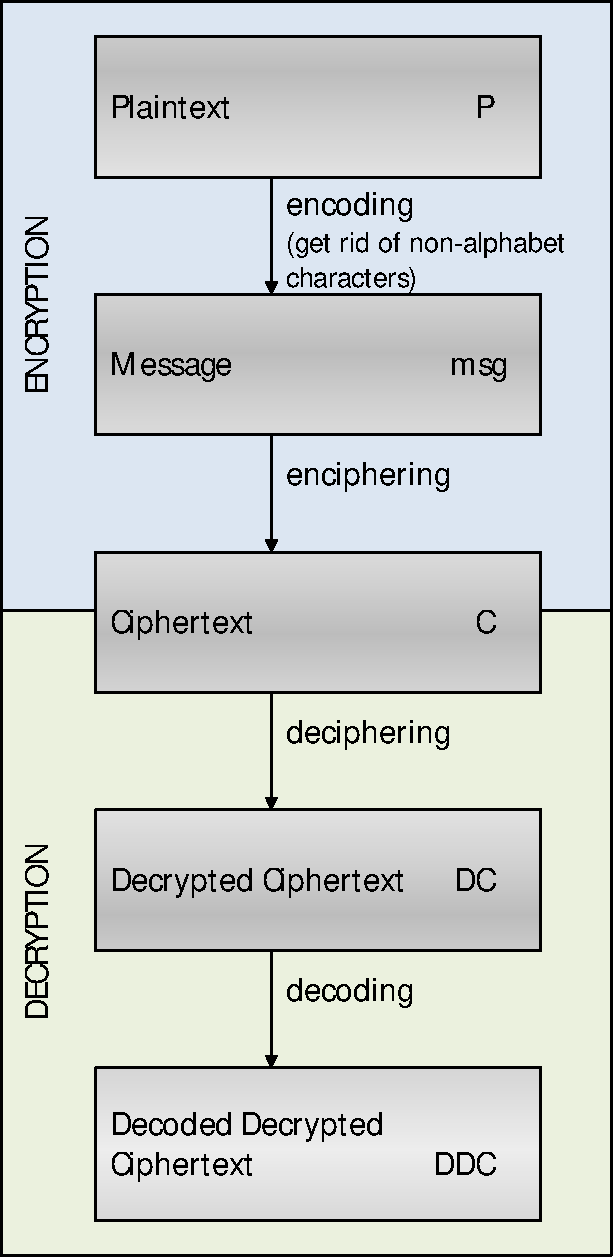
\includegraphics[scale=0.5]{figures/encryption-decryption-en}
\caption{Structure and naming convention of the Sage cipher code examples} 
\label{XXX}
\end{center}
\end{figure}



% ---------------------------------------------------------------------------
\newpage
\subsection{Transposition ciphers}

Transposition ciphers are implemented in the Sage class
\begin{center}
\verb!sage.crypto.classical.TranspositionCryptosystem!
\end{center}
To construct and work with a transposition cipher, we first need to
determine the alphabet that contains the symbols used to build the space of our plaintext
and ciphertext. 
Typically, this alphabet will be the upper-case letters of the
English alphabet, which can be accessed via the function
\begin{center}
\verb!sage.monoids.string_monoid.AlphabeticStrings!
\end{center}
We then need to decide on the block length of a block permutation,
which is the length of the row vector to be used in the simple columns
transposition. This row vector is our key, and it specifies a permutation
of a plaintext.

The following first example of transposition ciphers has block length 14,
and the key is build in a way, that every letter
in the plaintext is shifted to the right by two characters, with wrap
around at the end of the block. That is the encryption process. The decryption process is
shifting each letter of the ciphertext to the left by $14 - 2 = 12$.

\begin{sagecode}
\begin{Verbatim}%
[fontsize=\footnotesize,fontshape=tt]
sage: # transposition cipher using a block length of 14
sage: T = TranspositionCryptosystem(AlphabeticStrings(), 14)
sage: # given plaintext
sage: P   = "a b c d e f g h i j k l m n"
sage: # encryption key
sage: key = [3, 4, 5, 6, 7, 8, 9, 10, 11, 12, 13, 14, 1, 2]
sage:
sage: # encode plaintext (get rid of non-alphabet chars, convert lower-case to upper-case)
sage: msg = T.encoding(P)
sage: # encrypt plaintext by shifting to the left by 2 letters (do it in two steps)
sage: E   = T(key)
sage: C   = E(msg); C
CDEFGHIJKLMNAB
sage:
sage: # decrypt ciphertext by shifting to the left by 12 letters
sage: keyInv = [13, 14, 1, 2, 3, 4, 5, 6, 7, 8, 9, 10, 11, 12]
sage: D   = T(keyInv)
sage: D(C)
ABCDEFGHIJKLMN
sage:
sage: # Representation of key and inverse key as permutations
sage: E
(1,3,5,7,9,11,13)(2,4,6,8,10,12,14)
sage: D
(1,13,11,9,7,5,3)(2,14,12,10,8,6,4)
\end{Verbatim}
\caption{Simple Transposition by shifting (key and inverse key explicitly given)}
\end{sagecode}

\newpage
The second example of transposition ciphers is also a simple shifting column transposition.
But now the code is a little bit more automated: The keys are generated from the shift parameter.

\begin{sagecode}
\begin{Verbatim}%
[fontsize=\footnotesize,fontshape=tt]
sage: # transposition cipher using a block length of 14, code more variable
sage: keylen = 14
sage: shift = 2
sage: A = AlphabeticStrings()
sage: T = TranspositionCryptosystem(A, keylen)
sage:
sage: # construct the plaintext string from the first 14 letters of the alphabet plus blanks
sage: # plaintext   = "A B C D E F G H I J K L M N"
sage: A.gens()
(A, B, C, D, E, F, G, H, I, J, K, L, M, N, O, P, Q, R, S, T, U, V, W, X, Y, Z)
sage: P=''
sage: for i in range(keylen): P=P + " " + str(A.gen(i))
....:
sage: P
' A B C D E F G H I J K L M N'
sage:
sage: # encryption key
sage: # key = [3, 4, 5, 6, 7, 8, 9, 10, 11, 12, 13, 14, 1, 2]
sage: key = [(i+shift).mod(keylen) + 1 for i in range(keylen)]; key
[3, 4, 5, 6, 7, 8, 9, 10, 11, 12, 13, 14, 1, 2]
sage:
sage: # encode plaintext (get rid of non-alphabet chars)
sage: msg = T.encoding(P)
sage: # encrypt plaintext by shifting to the left by 2 letters (do it in one step)
sage: C   = T.enciphering(key, msg); C
CDEFGHIJKLMNAB
sage:
sage: # decrypt ciphertext by shifting to the left by 12 letters
sage: # keyInv = [13, 14, 1, 2, 3, 4, 5, 6, 7, 8, 9, 10, 11, 12]
sage: shiftInv=keylen-shift;
sage: keyInv = [(i+shiftInv).mod(keylen) + 1 for i in range(keylen)]; keyInv
[13, 14, 1, 2, 3, 4, 5, 6, 7, 8, 9, 10, 11, 12]
sage: DC   = T.enciphering(keyInv, C); DC
ABCDEFGHIJKLMN
sage:
sage: # decryption using the "deciphering method with key" instead of "enciphering with keyInv" 
sage: # using the deciphering method requires to change the type of the variable key
sage: DC  = T.deciphering(T(key).key(), C); DC
ABCDEFGHIJKLMN
sage:
sage: # representation of key and inverse key as permutations
sage: T(key)
(1,3,5,7,9,11,13)(2,4,6,8,10,12,14)
sage: T(key).key()
(1,3,5,7,9,11,13)(2,4,6,8,10,12,14)
sage: T(keyInv)
(1,13,11,9,7,5,3)(2,14,12,10,8,6,4)
\end{Verbatim}
\caption{Simple Transposition by shifting (key and inverse key constructed with "range")}
\end{sagecode}

\newpage
In the third example of transposition ciphers we use an arbitrary permutation as key in the
encryption and decryption processes in order to scramble the characters within each
block (block length = number of columns in a simple column transposition).
If the block length is $n$, then the key must be a permutation on $n$ symbols.
The following example uses the method \verb!random_key()! of the class
\verb!TranspositionCryptosystem!. Each call to \verb!random_key()! produces a
different key. Note that therefore your results (key and ciphertext) may be different
from the following example.

\begin{sagecode}
\begin{Verbatim}%
[fontsize=\footnotesize,fontshape=tt]
sage: # Remark: Enciphering here requires, that the length of msg is a multiple of keylen
sage: keylen = 14   # length of key
sage: A = AlphabeticStrings()
sage: T = TranspositionCryptosystem(A, keylen); T
Transposition cryptosystem on Free alphabetic string monoid on A-Z of block length 14
sage:
sage: P = "a b c d e f g h i j k l m n o p q r s t u v w x y z a b"
sage: key = T.random_key(); key
(1,2,3,13,6,5,4,12,7)(11,14)
sage: msg = T.encoding(P); msg
ABCDEFGHIJKLMNOPQRSTUVWXYZAB
sage: C   = T.enciphering(key, msg); C
BCMLDEAHIJNGFKPQAZRSOVWXBUTY
sage: # decryption using the "deciphering method with key" instead of "enciphering with keyInv" 
ssage: DC  = T.deciphering(key, C); DC
ABCDEFGHIJKLMNOPQRSTUVWXYZAB
sage:
sage: # Just another way of decryption: Using "enciphering" with the inverse key
sage: keyInv = T.inverse_key(key); keyInv
(1,7,12,4,5,6,13,3,2)(11,14)
sage: DC     = T.enciphering(keyInv, C); DC
ABCDEFGHIJKLMNOPQRSTUVWXYZAB
sage:
sage: # Test correctness of decryption
sage: msg == DC
True
\end{Verbatim}
\caption{Simple Column Transposition with randomly generated (permutation) key}
\end{sagecode}


\newpage
The fourth example of transposition ciphers additionally shows the key space of a simple
column transposition.

\begin{sagecode}
\begin{Verbatim}%
[fontsize=\footnotesize,fontshape=tt]
sage: keylen = 14   # length of key
sage: A = AlphabeticStrings()
sage: T = TranspositionCryptosystem(A, keylen); T
Transposition cryptosystem on Free alphabetic string monoid on A-Z of block length 14
sage: T.key_space()
Symmetric group of order 14! as a permutation group
sage: # Remark: The key space is not quite correct as also permutations shorter than keylen are counted.
sage:
sage: P = "a b c d e f g h i j k l m n o p q r s t u v w x y z a b"
sage: key = T.random_key(); key
(1,2,7)(3,9)(4,5,10,12,8,13,11)(6,14)
sage: msg = T.encoding(P); msg
ABCDEFGHIJKLMNOPQRSTUVWXYZAB
sage:
sage: # enciphering in one and in two steps
sage: C   = T.enciphering(key, msg); C
BGIEJNAMCLDHKFPUWSXBOAQZRVYT
sage:
sage: enc = T(key); enc.key()
(1,2,7)(3,9)(4,5,10,12,8,13,11)(6,14)
sage: C = enc(msg); C
BGIEJNAMCLDHKFPUWSXBOAQZRVYT
sage:
sage: # deciphering
sage: DC  = T.deciphering(key, C); DC
ABCDEFGHIJKLMNOPQRSTUVWXYZAB
\end{Verbatim}
\caption{Simple Column Transposition (showing the key\_space)}
\end{sagecode}



% ---------------------------------------------------------------------------
\newpage
\subsection{Substitution ciphers}

Substitution cryptosystems are implemented in Sage in the class
\begin{center}
\verb!sage.crypto.classical.SubstitutionCryptosystem!
\end{center}

\noindent The following code sample uses Sage to construct a substitution
cipher with a random key. A random key can be generated using the
method \verb!random_key()! of the class
\texttt{SubstitutionCryp\-to\-system}. Different keys determine different
substitution ciphers. So each call to \verb!random_key()! returns
different results.

\begin{sagecode}
\begin{Verbatim}%
[fontsize=\footnotesize,fontshape=tt]
sage: # plaintext/ciphertext alphabet
sage: A   = AlphabeticStrings()
sage: S   = SubstitutionCryptosystem(A)
sage:
sage: P   = "Substitute this with something else better."
sage: key = S.random_key(); key
INZDHFUXJPATQOYLKSWGVECMRB
sage:
sage: # method encoding can be called from A or from T
sage: msg = A.encoding(P); msg
SUBSTITUTETHISWITHSOMETHINGELSEBETTER
sage: C   = S.enciphering(key, msg); C
WVNWGJGVGHGXJWCJGXWYQHGXJOUHTWHNHGGHS
sage:
sage: #### We now decrypt the ciphertext to recover our plaintext.
sage:
sage: DC  = S.deciphering(key, C); DC
SUBSTITUTETHISWITHSOMETHINGELSEBETTER
sage: msg == DC
True
\end{Verbatim}
\caption{Monoalphabetic Substitution with randomly generated key}
\end{sagecode}



% ---------------------------------------------------------------------------
\newpage
\subsection{Caesar cipher}

The following example uses Sage to construct a Caesar
cipher.

\begin{sagecode}
\begin{Verbatim}%
[fontsize=\footnotesize,fontshape=tt]
sage: # plaintext/ciphertext alphabet
sage: A = AlphabeticStrings()
sage: P = "Shift the alphabet three positions to the right."
sage:
sage: # construct Caesar cipher
sage: S = SubstitutionCryptosystem(A)
sage: key = A([3, 4, 5, 6, 7, 8, 9, 10, 11, 12, 13, 14, 15, 16, 17, 18, 19, \
....:          20, 21, 22, 23, 24, 25, 0, 1, 2])
sage:
sage: # encrypt message
sage: msg     = A.encoding(P); msg
SHIFTTHEALPHABETTHREEPOSITIONSTOTHERIGHT
sage: encrypt = S(key); encrypt
DEFGHIJKLMNOPQRSTUVWXYZABC
sage: C       = encrypt(msg); C
VKLIWWKHDOSKDEHWWKUHHSRVLWLRQVWRWKHULJKW
sage:
sage: #### Next, we recover the plaintext.
sage:
sage: # decrypt message
sage: keyInv = A([23, 24, 25, 0, 1, 2, 3, 4, 5, 6, 7, 8, 9, 10, 11, 12, 13, \
....:             14, 15, 16, 17, 18, 19, 20, 21, 22])
sage: decrypt = S(keyInv); decrypt
XYZABCDEFGHIJKLMNOPQRSTUVW
sage: DC      = decrypt(C); DC
SHIFTTHEALPHABETTHREEPOSITIONSTOTHERIGHT
sage: msg == DC
True
\end{Verbatim}
\caption{Caesar (substitution by shifting the alphabet; key explicitly given, step-by-step approach)}
\end{sagecode}


\newpage
\noindent The second Caesar sample does the same, but the code is more sophisticated/automated/var\-i\-a\-ble.

\begin{sagecode}
\begin{Verbatim}%
[fontsize=\footnotesize,fontshape=tt]
sage: # plaintext/ciphertext alphabet
sage: A = AlphabeticStrings()
sage: keylen = len(A.gens()); keylen
26
sage: shift  = 3
sage: P = "Shift the alphabet three positions to the right."
sage:
sage: # construct Caesar cipher
sage: S = SubstitutionCryptosystem(A)
sage: S
Substitution cryptosystem on Free alphabetic string monoid on A-Z
sage: # key = A([3, 4, 5, 6, 7, 8, 9, 10, 11, 12, 13, 14, 15, 16, 17, 18, 19, \
sage: #          20, 21, 22, 23, 24, 25, 0, 1, 2])
sage: key = [(i+shift).mod(keylen) for i in range(keylen)];
sage: key = A(key); key
DEFGHIJKLMNOPQRSTUVWXYZABC
sage: len(key)
26
sage:
sage: # encrypt message
sage: msg     = A.encoding(P); msg
SHIFTTHEALPHABETTHREEPOSITIONSTOTHERIGHT
sage: C       = S.enciphering(key, msg); C
VKLIWWKHDOSKDEHWWKUHHSRVLWLRQVWRWKHULJKW
sage:
sage: #### Next, we recover the plaintext.
sage:
sage: # decrypt message
sage: # keyInv = A([23, 24, 25, 0, 1, 2, 3, 4, 5, 6, 7, 8, 9, 10, 11, 12, 13, \
sage: #             14, 15, 16, 17, 18, 19, 20, 21, 22])
sage: shiftInv=keylen-shift;
sage: keyInv = [(i+shiftInv).mod(keylen) for i in range(keylen)];
sage: keyInv = A(keyInv); keyInv
XYZABCDEFGHIJKLMNOPQRSTUVW
sage: DC     = S.enciphering(keyInv, C); DC
SHIFTTHEALPHABETTHREEPOSITIONSTOTHERIGHT
sage:
sage: # Just another way of decryption: Using "deciphering" with the key
sage: DC     = S.deciphering(key, C); DC
SHIFTTHEALPHABETTHREEPOSITIONSTOTHERIGHT
sage:
sage: msg == DC
True
\end{Verbatim}
\caption{Caesar (substitution by shifting the alphabet; substitution keys are generated)}
\end{sagecode}



% ---------------------------------------------------------------------------
\newpage
\subsection{Substitution with symbols}

In the following Sage example the symbols are from the binary number
system. A monoalphabetic substitution cipher with a binary alphabet has very little
security: Because the plaintext/ciphertext alphabet has only the two elements
0 and 1, there are only two keys possible: (0 1) and (1 0). Remark: In each key of a
substitution cipher all symbols of the alphabet have to appear once.

\begin{sagecode}
\begin{Verbatim}%
[fontsize=\footnotesize,fontshape=tt]
sage: # the plaintext/ciphertext alphabet
sage: A = BinaryStrings()
sage: # substitution cipher over the alphabet A; no keylen argument possible
sage: S = SubstitutionCryptosystem(A); S
Substitution cryptosystem on Free binary string monoid
sage: # to have a substitute for each symbol, key has always the length of the alphabet
sage: key = S.random_key(); key
10
sage: len(key)
2
sage: P = "Working with binary numbers."
sage: # encryption
sage: msg = A.encoding(P); msg
01010111011011110111001001101011011010010110111001100111001000000111011101101\
00101110100011010000010000001100010011010010110111001100001011100100111100100\
1000000110111001110101011011010110001001100101011100100111001100101110
sage: C   = S.enciphering(key, msg); C
10101000100100001000110110010100100101101001000110011000110111111000100010010\
11010001011100101111101111110011101100101101001000110011110100011011000011011\
0111111001000110001010100100101001110110011010100011011000110011010001
sage: # decryption
sage: DC  = S.deciphering(key, C); DC
01010111011011110111001001101011011010010110111001100111001000000111011101101\
00101110100011010000010000001100010011010010110111001100001011100100111100100\
1000000110111001110101011011010110001001100101011100100111001100101110
sage: msg == DC
True
\end{Verbatim}
\caption{Monoalphabetic substitution with a binary alphabet}
\end{sagecode}



\newpage
The second sample of a monoalphabetic substitution with symbols uses  a larger alphabet
as plaintext/ciphertext space as the first sample. Here the hexadecimal number system
is used as substitution alphabet.

\begin{sagecode}
\begin{Verbatim}%
[fontsize=\footnotesize,fontshape=tt]
sage: A = HexadecimalStrings()
sage: S = SubstitutionCryptosystem(A)
sage: key = S.random_key(); key
2b56a4e701c98df3
sage: len(key)
16
sage: # Number of possible keys
sage: factorial(len(key))
20922789888000
sage: P   = "Working with a larger alphabet."
sage:
sage: msg = A.encoding(P); msg
576f726b696e6720776974682061206c617267657220616c7068616265742e
sage: C   = S.enciphering(key, msg); C
47e375e9e1efe75277e17ae052eb52e8eb75e7e47552ebe872e0ebe5e47a5f
sage: DC  = S.deciphering(key, C); DC
576f726b696e6720776974682061206c617267657220616c7068616265742e
sage: msg == DC
True
sage:
sage: # Conversion hex back to ASCII:
sage: # - AlphabeticStrings() and HexadecimalStrings() don't have according methods.
sage: # - So we used Python:
sage: #   - repr(DC) converts the StringMonoidElement DC to a string
sage: #     still containing hex symbols;
sage: #   - binascii.a2b_hex converts this hex string to an ASCII string.
sage: import binascii
sage: DDC = binascii.a2b_hex(repr(DC)); DDC
'Working with a larger alphabet.'
sage:
sage: P == DDC
True
\end{Verbatim}
\caption{Monoalphabetic substitution with a hexadecimal alphabet (and decoding in Py\-thon)}
\end{sagecode}



% ---------------------------------------------------------------------------
\newpage
\subsection{Vigen{\`e}re cipher}

The Vigen{\`e}re cipher is implemented in the Sage class
\begin{center}
\verb!sage.crypto.classical.VigenereCryptosystem!
\end{center}

\noindent For our ciphertext/plaintext space, we can work with the upper-case
letters of the English alphabet, the binary number system, the
octal number system, or the hexadecimal number system. Here is an
example using the class \verb!AlphabeticStrings!, which implements
the English capital letters.

\begin{sagecode}
\begin{Verbatim}%
[fontsize=\footnotesize,fontshape=tt]
sage: # construct Vigenere cipher
sage: keylen = 14
sage: A = AlphabeticStrings()
sage: V = VigenereCryptosystem(A, keylen); V
Vigenere cryptosystem on Free alphabetic string monoid on A-Z of period 14
sage:
sage: # alternative: given key: key = A('ABCDEFGHIJKLMN'); key
sage: key = V.random_key(); key
WSSSEEGVVAARUD
sage: len(key)
14
sage:
sage: # encoding
sage: P = "The Vigenere cipher is polyalphabetic."
sage: len(P)
38
sage: msg = V.encoding(P); msg     # alternative: msg = A.encoding(P); msg
THEVIGENERECIPHERISPOLYALPHABETIC
sage:
sage: # encryption [2 alternative ways (in two steps or in one): both work]
sage: # encrypt = V(key); encrypt
sage: # C = encrypt(msg); C
sage: C   = V.enciphering(key, msg); C
PZWNMKKIZRETCSDWJAWTUGTALGBDXWLAG
sage:
sage: # decryption
sage: DC  = V.deciphering(key, C); DC
THEVIGENERECIPHERISPOLYALPHABETIC
sage: msg == DC
True
\end{Verbatim}
\caption{Vigen{\`e}re cipher}
\end{sagecode}




% ---------------------------------------------------------------------------
\newpage
\subsection{Hill cipher}

The Hill~\cite{pp:Hill1929,pp:Hill1931} or matrix cipher is more
mathematically sophisticated than other ciphers mentioned in this
chapter. The encryption/decryption key of this cipher is an invertible
square matrix, and the plaintext/ciphertext is processed also as a matrix.
The encryption and decryption processes use matrix operations. The Hill
cipher is implemented in the Sage class
\begin{center}
\verb!sage.crypto.classical.HillCryptosystem!
\end{center}

In the following example our plaintext/ciphertext space is the
capital letters of the English alphabet. In the Hill cipher, each
letter of this alphabet is assigned a unique integer modulo 26.

\begin{sagecode}
\begin{Verbatim}%
[fontsize=\footnotesize,fontshape=tt]
sage: # construct a Hill cipher
sage: keylen = 19    # keylen = 3  # Alternative key length with non-random small key
sage: A = AlphabeticStrings()
sage: H = HillCryptosystem(A, keylen); H
Hill cryptosystem on Free alphabetic string monoid on A-Z of block length 19
sage:
sage: # To create key non-randomly, HKS is necessary [even H.key_space() is not enough].
sage: # HKS = H.key_space()
sage: # key = HKS([[1,0,1],[0,1,1],[2,2,3]]); key
sage:
sage: # Random key creation
sage: key = H.random_key(); key
[10  7  5  2  0  6 10 23 15  7 17 19 18  2  9 12  0 10 11]
[23  1  1 10  4  9 21  1 25 22 19  8 17 22 15  8 12 25 22]
[ 4 12 16 15  1 12 24  5  9 13  5 15  8 21 23 24 22 20  6]
[ 5 11  6  7  3 12  8  9 21 20  9  4 16 18 10  3  2 23 18]
[ 8 22 14 14 20 13 21 19  3 13  2 11 13 23  9 25 25  6  8]
[24 25  8 24  7 18  3 20  6 11 25  5  6 19  7 24  2  4 10]
[15 25 11  1  4  7 11 24 20  2 18  4  9  8 12 19 24  0 12]
[14  6  2  9 11 20 13  4 10 11  4 23 14 22 14 16  9 12 18]
[12 10 21  5 21 15 16 17 19 20  1  1 15  5  0  2 23  4 14]
[21 15 15 16 15 20  4 10 25  7 15  4  7 12 24  9 19 10  6]
[25 15  2  3 17 23 21 16  8 18 23  4 22 11 15 19  6  0 15]
[14 23  9  3 18 15 10 18  7  5 12 23 11  9 22 21 20  4 14]
[ 3  6  8 13 20 16 11  1 13 10  4 21 25 15 12  3  0 11 18]
[21 25 14  6 11  3 21  0 19 17  5  8  5  4  9  2 23 19 15]
[ 8 11  9 11 20 15  6  1  3 18 18 22 16 17  6  3 15 11  2]
[21 15  5 22  2  9  0  4 22 10  2 10 19 19 17 19  1 21  4]
[ 7 17  9  2 15  5 14  3  6  9 12 12 22 15  8  4 21 14 19]
[19 14 24 19  7  5 22 22 13 14  7 18 17 19 25  2  1 23  6]
[ 2  6 14 22 17  7 23  6 22  7 13 20  0 14 23 17  6  1 12]
sage:
sage: # encoding and encryption
sage: P = "Hill or matrix cipher uses matrix operations."
sage: len(P)
45
sage: # implementation requires: Length of msg is a multiple of matrix dimension (block_length)
sage: msg = H.encoding(P); msg
HILLORMATRIXCIPHERUSESMATRIXOPERATIONS
sage: len(msg)
38
sage:
sage: # encryption
sage: C  = H.enciphering(key, msg); C
CRWCKPRVYXNBRZTNZCTQWFWSDWBCHABGMNEHVP
sage:
sage: # decryption
sage: DC  = H.deciphering(key, C); DC
HILLORMATRIXCIPHERUSESMATRIXOPERATIONS
sage: msg == DC
True
sage:
sage: # alternative decryption using inverse matrix
sage: keyInv = H.inverse_key(key); keyInv
[ 6 23  1 23  3 12 17 22  6 16 22 14 18  3  1 10 21 16 20]
[18 23 15 25 24 23  7  4 10  7 21  7  9  0 13 22  5  5 23]
...
[10 11 12  6 11 17 13  9 19 16 14 24  4  8  5 16 18 20  1]
[19 16 16 21  1 19  7 12  3 18  1 17  7 10 24 21  7 16 11]
sage: DC     = H.enciphering(keyInv, C); DC
HILLORMATRIXCIPHERUSESMATRIXOPERATIONS
\end{Verbatim}
\caption{Hill cipher}
\end{sagecode}







% --------------------------------------------------------------------------
\newpage
\begin{thebibliography}{99999}
\addcontentsline{toc}{section}{Bibliography}

\bibitem[ACA2002]{pp:ACA2002} \index{ACA 2002}
   American Cryptogram Association, \\
   {\em Length and Standards for all ACA Ciphers}, \\
   2002.\\
   \href{http://www.cryptogram.org/cdb/aca.info/aca.and.you/chap08.html#}
   {\texttt{http://www.cryptogram.org/cdb/aca.info/aca.and.you/chap08.html\#}}

\bibitem[Bauer1995]{pp:Bauer1995} \index{Bauer 1995}
    Friedrich L. Bauer, \\
    {\em Entzifferte Geheimnisse}, Springer, 1995.

\bibitem[Bauer2000]{pp:Bauer2000} \index{Bauer 2000}
    Friedrich L. Bauer, \\
    {\em Decrypted Secrets}, Springer 1997, 2nd edition 2000.
	
\bibitem[Crowley2000]{pp:Crowley2000} \index{Crowley 2000}
   Paul Crowley, \\
   {\em Mirdek: A card cipher inspired by ``Solitaire''}, \\
   2000.\\
   \href{http://www.ciphergoth.org/crypto/mirdek/}
   {\texttt{http://www.ciphergoth.org/crypto/mirdek/}}

\bibitem[DA1999]{pp:DA1999} \index{DA 1999}
   Data encryption page of the ThinkQuest Team 27158 for ThinkQuest 1999 \\
   (no update since 1999, no search possibility), \\
   1999.\\
   \href{http://library.thinkquest.org/27158/}
   {\texttt{http://library.thinkquest.org/27158/}}

\bibitem[Goebel2003]{pp:Goebel2003} \index{Goebel 2003}
   Greg Goebel, \\
   {\em Codes, Ciphers and Codebreaking}, \\
   2003.\\
   \href{http://www.vectorsite.net/ttcode.htm}
   {\texttt{http://www.vectorsite.net/ttcode.htm}}

\bibitem[Hill1929]{pp:Hill1929} \index{Hill 1929}
   Lester S. Hill,\\
   ``Cryptography in an Algebraic Alphabet,''
   \emph{The American Mathematical Monthly}, 36(6):306--312, 1929.

\bibitem[Hill1931]{pp:Hill1931} \index{Hill 1931}
   Lester S. Hill,\\
   ``Concerning Certain Linear Transformation Apparatus of Cryptography,''
   \emph{The American Mathematical Monthly}, 38(3):135--154, 1931.

\bibitem[Nichols1996]{pp:Nichols1996} \index{Nichols 1996} 
    Randall K. Nichols, \\
    {\em Classical Cryptography Course, Volume 1 and 2}, \\
    Aegean Park Press 1996;
    or in 12 lessons online at \\
    \href{http://www.fortunecity.com/skyscraper/coding/379/lesson1.htm}
    {\texttt{http://www.fortunecity.com/skyscraper/coding/379/lesson1.htm}}

\bibitem[Savard1999]{pp:Savard1999} \index{Savard 1999}
	John J. G. Savard, \\
	{\em A Cryptographic Compendium}, \\
	1999.\\
	\href{http://www.hypermaths.org/quadibloc/crypto/jscrypt.htm}
	{\texttt{http://www.hypermaths.org/quadibloc/crypto/jscrypt.htm}}
	
\bibitem[Schmeh2004]{pp:Schmeh2004}  \index{Schmeh 2004}
        Klaus Schmeh, \\
        {\em Die Welt der geheimen Zeichen. Die faszinierende Geschichte
        der Verschl\"usselung},\\ 
        W3L Verlag Bochum, 1. Auflage 2004.

\bibitem[Schmeh2007]{pp:Schmeh2007}  \index{Schmeh 2007}
        Klaus Schmeh, \\
        {\em Codeknacker gegen Codemacher. Die faszinierende Geschichte der Verschl\"usselung.},\\ 
        W3L Verlag Bochum, 2. Auflage 2007.\\
	This is most current among the books dealing in a comprehensive manner
	with the history of cryptology. It contains a small collection of solved
	and unsolved crypto riddles. One of the challenges deals with a double
	column transposition using two long keys, which are differently in addition.

\bibitem[Schneier1999]{pp:Schneier1999}
	Bruce Schneier, \\
	{\em The Solitaire Encryption Algorithm}, \\
	version 1.2, 1999.\\
	\href{http://www.schneier.com/solitaire.html}
	{\texttt{http://www.schneier.com/solitaire.html}}

\bibitem[Singh2001]{pp:Singh2001} \index{Singh 2001}
	Simon Singh, \\
	{\em Geheime Botschaften. Die Kunst der Verschl\"usselung von der 
        Antike bis in die Zeiten des Internet}, \\
	dtv, 2001.

\bibitem[ThinkQuest1999]{pp:ThinkQuest1999} \index{ThinkQuest 1999}
	ThinkQuest Team 27158, \\
	{\em Data Encryption}, \\
	1999.\\
	\href{http://library.thinkquest.org/27158/}
	{\texttt{http://library.thinkquest.org/27158/} }

\end{thebibliography}









% Local Variables:
% TeX-master: "../script-en.tex"
% End:


% $Id$
%%%%%%%%%%%%%%%%%%%%%%%%%%%%%%%%%%%%%%%%%%%%%%%%%%%%%%%%%%%%%%%%%%%%%%%%%%
%
% C H A P T E R   T H R E E :  P R I M E S
%
%%%%%%%%%%%%%%%%%%%%%%%%%%%%%%%%%%%%%%%%%%%%%%%%%%%%%%%%%%%%%%%%%%%%%%%%%%

\newpage
\hypertarget{Kapitel_2}{}
\section{Prime Numbers}
\label{Label_Kapitel_2}
(Bernhard Esslinger, May 1999; Updates Nov. 2000, Dec. 2001, June 2003, May 2005, March 2006, May 2007)

\begin{center}
\fbox{\parbox{15cm}{
    \emph{Albert Einstein\footnotemark:}\\
    Progress requires exchange of knowledge.
}}
\end{center}
\addtocounter{footnote}{0}\footnotetext{%
  Albert Einstein, German physicist and Nobel Prize winner, 
  Mar 14, 1879 $-$ Apr 14, 1955.
}

% --------------------------------------------------------------------------
\subsection{What are prime numbers?}
\index{Prime number} \index{Number!prime}
Prime numbers are whole, positive numbers greater than or equal to $2$ that can
only be divided by 1 and themselves. All other natural numbers greater than or
equal to $2$ can be formed by multiplying prime numbers.

The {\em natural} \index{Number!natural} numbers $\mathbb{N}=\{1, 2, 3, 4,\cdots \}$ thus comprise 
\begin{itemize}
   \item the number $1$ (the unit value)
   \item the primes and
   \item the composite numbers.
\end{itemize}

Prime numbers are particularly important for 3 reasons:
\begin{itemize}
  \item In number theory, they are considered to be the basic components of
natural numbers, upon which numerous brilliant mathematical ideas are based.
  \item They are of extreme practical importance in modern
\index{Cryptography!modern} cryptography (public key \index{Cryptography!public key} cryptography). The most common public key procedure, invented at the end of
the 1970's, is \index{RSA} RSA encryption. Only using (large) prime numbers for
particular parameters can you guarantee that an algorithm is secure, both for
the RSA procedure and for even more modern procedures (digital
\index{Signature!digital} signature, elliptic curves).
  \item The search for the largest known prime numbers does not have any
practical usage known to date, but requires the best computers, is an excellent
benchmark (possibility for determining the performance\index{Performance} of computers) and leads
to new calculation methods on many computers \\ (see also:
\href{http://www.mersenne.org/prime.htm}{\tt
http://www.mersenne.org/prime.htm}).
\end{itemize}
Many people have been fascinated by prime numbers over the past two millennia.
Ambition to make new discoveries about prime numbers has often resulted in
brilliant ideas and conclusions. The following section provides an easily
comprehensible introduction to the basics of prime numbers. We will also explain
what is known about the distribution (density, number of prime numbers in
particular intervals) of prime numbers and how prime number tests work.


% --------------------------------------------------------------------------
\subsection{Prime numbers in mathematics}\label{primesinmath}

Every whole number has a factor. The number 1 only has one factor,
itself, whereas the number $12$ has the six factors $1, 2, 3, 4,
6, 12$. Many numbers can only be divided by themselves and by $1$.
With respect to multiplication, these are the ``atoms'' in the
area of numbers. Such numbers are called prime numbers.

In mathematics, a slightly different (but equivalent) definition is used.

\begin{definition}\label{def-pz-prime}
A whole number $p \in {\bf N}$ is called prime \index{Number!prime} if
$p > 1$ and $p$ only possesses the trivial factors $\pm 1$ and $\pm p$.
\end{definition}


By definition, the number $1$ is not a prime number. In the following sections,
$p$ will always denote a prime number.

The sequence of prime numbers starts with $$ 2,~ 3,~ 5,~ 7, ~ 11, ~ 13, ~
17, ~ 19, ~ 23, ~ 29, ~ 31, ~ 37, ~ 41, ~ 43, ~ 47, ~ 53, ~ 59, ~ 61,
~ 67, ~ 71, ~ 73, ~ 79, ~ 83, ~ 89, ~ 97, \cdots . $$
The first 100 numbers include precisely 25 prime numbers. After this,
the percentage of primes constantly decreases. Prime numbers can be
factorised in a uniquely {\em trivial} way: 
$$5 = 1 \cdot 5,\quad  17 = 1 \cdot 17, \quad 1,013 = 1 \cdot 1,013,  \quad
1,296,409 = 1 \cdot 1,296,409.$$
All numbers that have $2$ or more factors not equal 1 are called 
\index{Number!composite} {\em composite} numbers. 
These include $$ 4 = 2 \cdot 2, \quad 6 = 2\cdot 3 $$ as well
as numbers that {\em look like primes}, but are in fact composite:
$$ 91 = 7 \cdot 13, \quad 161=7 \cdot 23, \quad 767 =13 \cdot 59. $$

\begin{theorem}\label{thm-pz-sqr}
Each whole number $m$ greater than $1$ possesses a lowest factor greater than
$1$. This is a prime number $p$. Unless $m$ is a prime number itself, then: $p$
is less than or equal to the square root of $m$.
\end{theorem}

All whole numbers greater than $1$ can be expressed as a product of prime
numbers --- in a unique way. This is the claim of the 1st fundamental theorem of
number theory (= fundamental theorem of arithmetic = fundamental building block
of all positive integers).\index{Number theory!fundamental theorem}

\begin{theorem}\label{thm-pz-prod}
Each element $n$ of the natural numbers greater than $1$ can be written as the
product $n = p_1 \cdot p_2 \dots p_m$ of prime numbers. If two such
factorisations $$n =  p_1 \cdot p_2 \cdot \cdots \cdot p_m = p'_1 \cdot p'_2 \cdots
p'_{m'}$$ are given, then they can be reordered such that $\;m = m'\;$ and for
all $i$:  $\;p_i = p'_i$. \\
($p_1, p_2, \dots, p_m$ are called the prime factors of n).
\end{theorem}

In other words: each natural number other than $1$ can be written as a product
of prime numbers in precisely one way, if we ignore the order of the factors.
The factors are therefore unique (the {\em expression as a product of factors}
is unique)! For example, $$ 60 = 2 \cdot 2 \cdot 3 \cdot 5 = 2^2\cdot 3^1 \cdot
5^1. $$
And this --- other than changing the order of the factors --- is the only way in
which the number $60$ can be factorised. If you allow numbers other than primes
as factors, there are several ways of factorising integers and the uniqueness \hypertarget{uniqueness}{} is
lost: $$ 60 = 1 \cdot 60 = 2 \cdot 30 = 4 \cdot 15 = 5 \cdot 12 =6 \cdot 10 = 2
\cdot 3 \cdot 10 = 2 \cdot 5 \cdot 6 = 3 \cdot 4 \cdot 5 = \cdots . $$

The following section is aimed more at those familiar with mathematical logic:
The 1st fundamental theorem only appears to be obvious \label{remFundTheoOfArithm}. We can construct
numerous other sets of numbers (i.e. other than positive whole numbers greater
than 1), for which numbers in the set cannot be expressed uniquely as a product
of the prime numbers of the set: In the set $M = \{1, 5, 10, 15, 20, \cdots\}$
there is no equivalent to the fundamental theorem under multiplication. The
first five prime numbers of this sequence are $5, 10, 15, 20, 30$ (note: $10$ is
prime, because $5$ is not a factor of $10$ in this set --- the result is not an
element of the given basic set $M$). Because the following applies in $M$: $$
100 = 5 \cdot 20 = 10 \cdot 10 $$ and $5, 10, 20$ are all prime numbers in this
set, the expression as a product of prime factors is not unique here.

% --------------------------------------------------------------------------
\subsection{How many prime numbers are there?}

For the natural numbers, the primes can be compared to elements in chemistry or
the elementary particles in physics (see \cite[p. 22]{Blum1999}).

Although there are only $92$ natural chemical elements, the number of prime
numbers is unlimited. Even the Greek, \index{Euclid} Euclid%
\footnote{Euclid,
a Greek mathematician of 4th and 3rd century B.C. He worked at the
Egyptian academy of Alexandria and wrote ``The Elements'', the most well 
known systematically textbook of the Greek mathematics.} 
knew this in the third century B.C.
\begin{theorem}[Euclid\footnote{The common usage of the term does not denote Euclid as the inventor of the theorem rather;
the true inventor is merely not as prominent. The theorem has already been distinguished
and proven in Euclid's Elements (Book IX, theorem 20). The phraseology is remarkable due to 
the fact that the word infinite is not used. The text reads as followed
$$
O\acute{\iota}~\pi\varrho\tilde{\omega}\tau o \iota~\grave{\alpha}\varrho\iota\vartheta\mu o\grave{\iota}~
\pi\lambda\varepsilon\acute{\iota}o \upsilon\varsigma~\varepsilon\grave{\iota}\sigma\grave{\iota}~
\pi\alpha\nu\tau\grave{o}\varsigma~\tau o \tilde{\upsilon}~
\pi\varrho o \tau\varepsilon\vartheta\acute{\varepsilon}\nu\tau o \varsigma~
\pi\lambda\acute{\eta}\vartheta\ o \upsilon\varsigma~
\pi\varrho\acute{\omega}\tau\omega\nu~
\grave{\alpha}\varrho\iota\vartheta\mu\tilde{\omega}\nu,
$$
the English translation of which is: the prime numbers are more than 
any previously existing amount of prime numbers.
}]\label{thm-pz-euklid} % Ende der Fu�note
% Fussnote VOR "]" in [Euclid], damit kein Leerraum vor der Fussnotennummer.
% Vorher stand da: ...(Euclid). BLANK Fussnote und das Blank stoerte.
% Nun steht die Fussnote direkt hinter "Euclid" und vor der ")".
% Eigentlich h�tte ich sie gerne direkt hinter "(Euclid)", noch vor dem 
% automatisch gesetzten Punkt. 
The sequence of prime numbers does not discontinue.
Therefore, the quantity of prime numbers is infinite.
\end{theorem}
His proof that there is an infinite number of
primes is still considered to be a brilliant mathematical consideration and
conclusion today (proof by contradiction \index{Proof by contradiction}). 
He assumed that there is only a finite number of primes and therefore a 
largest prime number. Based on this assumption, he drew logical conclusions
until he obtained an obvious contradiction. This meant that something must
be wrong. As there were no mistakes in the chain of conclusions, it could
only be the assumption that was wrong. Therefore, there must be an infinite
number of primes!

\hypertarget{euclid}{}
\paragraph{Euclid's proof by contradiction}
\index{Euclid's proof by contradiction}\index{Proof by contradiction}
goes as follows:

\begin{Proof}{}
{\bf Assumption:} \quad There is a {\em finite} number of primes. \\*[4pt] {\bf
Conclusion:} \quad Then these can be listed $p_1 < p_2 < p_3 < \dots < p_n$,
where $n$ is the (finite) number of prime numbers. $p_n$ is therefore the
largest prime. Euclid now looks at the number $a = p_1 \cdot p_2 \cdots p_n +1$.
This number cannot be a prime number because it is not included in our list of
primes. It must therefore be divisible by a prime, i.e. there is a natural
number $i$ between $1$ and $n$, such that $p_i$ divides the number $a$. Of
course, $p_i$ also divides the product $a-1 = p_1 \cdot p_2 \cdots p_n$, because
$p_i$ is a factor of $a-1$. Since $ p_i $ divides the numbers $ a $ and $ a-1 $,
it also divides the difference of these numbers. Thus: $p_i$ divides  $a - (a-1)
= 1$. $p_i$ must therefore divide $1$, which is impossible. \\*[4pt] {\bf
Contradiction:} \quad Our assumption was false.

Thus there is an {\em infinite} number of primes
(Cross-reference: \hyperlink{primhfk}{overview} under \ref{s:primhfk} of 
the number of prime numbers in various intervals).
\end{Proof} 

\par \vskip + 10pt

Here we should perhaps mention yet another fact which is initially somewhat surprising. 
Namely, in the prime numbers sequence $p_1, p_2, \cdots,$ gaps between prime numbers can have
an individually determined length $n$. It is undeniable that under the $n$
succession of natural numbers
$$(n+1)!+2,\cdots, (n+1)!+(n+1),
$$
none of them is a prime number since in order, the numbers $2,3,\cdots,(n+1)$  
are comprised respectively as real divisors. 
($n!$ means the product of the first $n$ natural numbers therefore 
$ n!= n*(n-1)*\cdots *2*1$).


% --------------------------------------------------------------------------
% --------------------------------------------------------------------------
\vskip + 20pt
\subsection{The search for extremely large primes}
\label{search_for_very_big_primes}   % chap. 3.4

The largest prime numbers known today have several millions digits, 
which is too big for us to imagine. The number of elementary particles in
the universe is estimated to be ``only'' a $80$-digit number 
\hyperlink{grosord}{(See: overview under \ref{s:grosord}
of various orders of magnitude / dimensions)}.


% --------------------------------------------------------------------------
\hypertarget{RecordPrimes}{}
\subsubsection{The 20 largest known primes (as of May 2007)}  % Eyecatcher_neue-Mersenne
\label{RecordPrimes}
\index{Prime number!records}

The following table contains the current record primes and
a description of its particular number type\footnote{%
An up-to-date version can be found in the internet at
     \href{http://primes.utm.edu/largest.html}
  {\texttt{http://primes.utm.edu/largest.html}}.
}:

\index{Mersenne!number!generalized}
\index{Fermat!number!generalized} 

\begin{table}[h]
\begin{center}
\begin{tabular}{|c|cccc|}
\hline    % Eyecatcher_neue-Mersenne
	& {\bf Definition} & {\bf Decimal Digits} & {\bf When} & {\bf Description} \\
\hline
	1  & $2^{32,582,657}-1$ & 9,808,358 & 2006 & Mersenne, 44th known \\
	2  & $2^{30,402,457}-1$ & 9,152,052 & 2005 & Mersenne, 43rd known \\
	3  & $2^{25,964,951}-1$ & 7,816,230 & 2005 & Mersenne, 42nd known \\
	4  & $2^{24,036,583}-1$ & 7,235,733 & 2004 & Mersenne, 41st known \\
	5  & $2^{20,996,011}-1$ & 6,320,430 & 2003 & Mersenne, 40th known \\
	6  & $2^{13,466,917}-1$ & 4,053,946 & 2001 & Mersenne, M-39 \\
	7  & $19,249 \cdot 2^{13,018,586}+1$ & 3,918,990 & 2007 & Generalized Mersenne\footnotemark \\
	8  & $27,653 \cdot 2^{9,167,433}+1$ & 2,759,677 & 2005 & Generalized Mersenne \\



	9  & $28,433 \cdot 2^{7,830,457}+1$ & 2,357,207 & 2004 & Generalized Mersenne \\

	10  & $2^{ 6,972,593}-1$ & 2,098,960 & 1999 & Mersenne, M-38 \\
	11  & $5,359 \cdot 2^{5,054,502}+1$ & 1,521,561 & 2003 & Generalized Mersenne \\

	12  & $4,847 \cdot 2^{3,321,063}+1$ & 999,744 & 2005 & Generalized Mersenne \\
	13  & $3 \cdot 2^{3,136,255}-1$ & 944,108 & 2007 & Generalized Mersenne \\

	14  & $2^{ 3,021,377}-1$ &   909,526 & 1998 & Mersenne, M-37 \\
	15  & $2^{ 2,976,221}-1$ &   895,932 & 1997 & Mersenne, M-36 \\

	16  & $222,361 \cdot 2^{2,854,840}+1$ & 859,398 & 2006 & Generalized Mersenne \\

	17 & $1,372,930^{131,072}+1$ &   804,474 & 2003 & Generalized Fermat\footnotemark \\

	18  & $1,361,244^{131,072}+1$ &   803,988 & 2004 & Generalized Fermat \\
	19  & $1,176,694^{131,072}+1$ &   795,695 & 2003 & Generalized Fermat \\

	20  & $342,673 \cdot 2^{2,639,439}-1$ & 794,556 & 2007 & Generalized Mersenne \\

\hline
\end{tabular}
\caption{The 20 largest known primes and its particular number types
         (as of May 2007)}    % Eyecatcher_neue-Mersenne
\label{L_n_Largest_Kown-Primes}
\end{center}
\end{table} 
\footnotetext{\index{Number!Sierpinski}\index{Seventeen or Bust SoB}%
This number was found within the distributed computing project
``Seventeen or Bust'' (SoB) (\href{http://www.seventeenorbust.com}{\texttt{http://www.seventeenorbust.com}})
% {\href{http://www.mersenne.org} {\tt http://www.mersenne.org}}
at March 26, 2007. While the well known \hyperlink{GIMPS-project}{GIMPS project} (chapter~\ref{zahlentyp_mersenne}) searches for bigger and bigger of the infinitely many primes, there is a chance, that the SoB project could have been completed its
task sometime.

The SoB project tries to prove computationally, that the number $k = 78,557$ is
the smallest Sierpinski number (John Selfridge proved in 1962, that $78,557$ is a Sierpinski number).

The famous Polish mathematician Waclaw Sierpinski (1882 to 1969) proved in
1960, that there exist infinitely many odd integers k, which fulfill the
following property: For all Sierpinski numbers k it is true: All numbers $N = k \cdot 2^{n}+1$ are composite for all integers $n>=1$ (Sierpinski's Composite Number Theorem, \href{http://mathworld.wolfram.com/SierpinskisCompositeNumberTheorem.html}{\texttt{http://mathworld.wolfram.com/SierpinskisCompositeNumberTheorem.html}}).

When the project started in 2002 there have been 17 possible candidates $< 78557$ (this is the reason for the project's name ``Seventeen or Bust''). It is sufficient to find one single counter-example, to exclude a candidate k, which means to find a single $n>=1$, where $N = k \cdot 2^{n}+1$ is prime. So it is only a byproduct of this task that this also generates new monster primes.
} 
\footnotetext{%
Generalized Fermat number: $ 1,372,930^{131,072} + 1 = 1,372,930^{(2^{17})}+1 $
\index{Fermat!number!generalized}  } 
%be_2005: Erzwingen, dass die Abb. noch in diesem Kapitel !

The largest known prime is a Mersenne prime, found by the
\hyperlink{GIMPS-project}{GIMPS project}(chapter~\ref{zahlentyp_mersenne}).

Within the largest known primes there are also numbers of the type
\hyperlink{generalizedMersennenumbers}{generalized Mersenne number}
(chapter~\ref{generalized-mersenne-no1})
and 
\hyperlink{generalizedFermatprimes}{generalized Fermat numbers}
(chapter~\ref{generalized-fermat}).


% --------------------------------------------------------------------------
\hypertarget{MersenneNumbers01}{}
\subsubsection{Special number types -- Mersenne numbers and Mersenne primes} 
\label{zahlentyp_mersenne}
\index{Mersenne!number}

Almost all known huge prime numbers are special candidates, called
\index{Mersenne, Marin} {\em Mersenne numbers}\footnote{%
Marin Mersenne, French priest and mathematician, Sep 08, 1588 $-$ Sep 01, 1648.
\index{Mersenne, Marin}
}
of the form $2^p -1,$ where $p$ is
a prime. Not all Mersenne numbers are prime:

$$
\begin{array}{cl}
2^2 - 1 = 3 & \Rightarrow {\rm prime} \\
2^3 - 1 = 7 & \Rightarrow {\rm prime} \\
2^5 - 1 = 31    & \Rightarrow {\rm prime} \\
2^7 - 1 = 127    & \Rightarrow {\rm prime} \\
2^{11} - 1 = 2,047 = 23 \cdot 89    & \Rightarrow  {\rm NOT~prime} !
\end{array}
$$

\index{Number!Mersenne}\index{Mersenne!number}
\index{Mersenne!theorem} 

Even Mersenne knew that not all Mersenne numbers
are prime (see exponent $p = 11$). 
A prime Mersenne number \index{Mersenne!prime number} is called
Mersenne prime number.  \\
However, he is to be thanked for the interesting conclusion that a number 
of the form $2^n-1$ cannot be a prime number if $n$ is a composite number:

\begin{theorem}[Mersenne]\label{thm-pz-mersenne} 
  If $2^n - 1$ is a prime number, then $n$ is also a prime number.
\end{theorem}

\begin{Proof}{}
The theorem of Mersenne can be proved by contradiction%
\index{Proof by contradiction}.  We therefore assume that
there exists a composite natural number $ n $ (with real factorisation)  
$ n=n_1 \cdot n_2 $
, with the property that $ 2^n -1 $ is a prime number.

From \begin{eqnarray*} (x^r-1)((x^r)^{s-1} + (x^r)^{s-2} + \cdots + x^r +1) & =
&  ((x^r)^s + (x^r)^{s-1} + (x^r)^{s-2} + \cdots + x^r) \\ &  & -((x^r)^{s-1} +
(x^r)^{s-2} + \cdots + x^r +1)  \\ & = & (x^r)^s -1 = x^{rs } -1,
\end{eqnarray*} we conclude \[ 2^{n_1 n_2} - 1 = (2^{n_1} -1)((2^{n_1})^{n_2 -1}
+ (2^{n_1})^{n_2 -2} + \cdots + 2^{n_1} + 1). \]
Because $ 2^n - 1 $ is a prime number, one of the above two factors on the
right-hand side must be equal to 1. This is the case if and only if $ n_1 =1 $
or $ n_2 =1$. But this contradicts our assumption. Therefore the assumption is
false. This means that there exists no composite number $ n, $ such that $ 2^n -
1 $ is a prime.
\end{Proof} 

\vskip + 5pt
\hypertarget{Mer-nums-not-always-prim}{}
Unfortunately this theorem only applies in one direction (the inverse 
statement does not apply, no equivalence): that means that there exist 
prime exponent for which the Mersenne number is {\bf not} prime (see the 
above example $2^{11}-1, $ where $11$ is prime, but $2^{11}-1$ not).

Mersenne claimed that $2^{67}-1$ is a prime number. There is also a mathematical
history behind this claim: it first took over 200 years before 
\index{Lucas, Edouard} Edouard Lucas (1842-1891) proved that this number 
is composite.
However, he argued indirectly and did not name any of the factors. Then Frank
Nelson Cole\index{Cole, Frank Nelson}\footnote{%
Frank Nelson Cole, American mathematician, Sep. 20, 1861 $-$ May 26, 1926.}
showed in 1903 which factors make up this composite number: 
$$ 2^{67} -1
=147, 573, 952, 589, 676, 412, 927 = 193, 707, 721 \cdot 761, 838, 257, 287. $$
He admitted to having worked 20 years on the factorisation 
\index{Factorisation} (expression as a product of prime factors)\footnote{%
  Using CrypTool\index{CrypTool} you can factorize numbers in the 
  following way: menu {\bf Indiv. Procedures \textbackslash{} RSA Cryptosystem 
  \textbackslash{} Factorisation of a Number}. \\
  CrypTool can factorize in a reasonable time numbers no longer than 250 bit.
  Numbers bigger than 1024 bits are currently not accepted by CrypTool. \\
  The current factorization records are listed in chapter \ref{NoteFactorisation}.
  \index{Factorisation!factoring records}
}
of this 21-digit decimal number!

Due to the fact that the exponents of the Mersenne numbers
\index{Mersenne!number} do not use all
natural numbers, but only the primes, the {\em experimental space} is limited
considerably. The currently known Mersenne prime numbers 
\index{Mersenne!prime number} have the exponents\footnote{%
The following page from Landon Curt Noll\index{Noll, Landon Curt} contains 
all Mersenne primes including its date of discovery and its value as number 
and as word:
      \href{http://www.isthe.com/chongo/tech/math/prime/mersenne.html}
   {\texttt{http://www.isthe.com/chongo/tech/math/prime/mersenne.html}}. \\
Also see:
      \href{http://www.utm.edu/}
   {\texttt{http://www.utm.edu/}}.
                             } 
$$
\begin{array}{c}
2; ~ 3; ~ 5; ~ 7; ~ 13; ~ 17; ~ 19; ~ 31; ~ 61; ~ 89; ~ 107; ~ 127;
~ 521; ~ 607; ~ 1,279; ~ 2,203; ~ 2,281; ~ 3,217; ~ 4,253;\\
 4,423; ~ 9,689; ~ 9,941, ~ 11,213; ~ 19,937; ~ 21,701; ~ 23,207; ~ 44,497; ~
86,243; ~ 110,503; ~ 132,049; \\
 216,091; ~ 756,839; ~ 859,433; ~ 1,257,787; ~ 1,398,269; ~ 2,976,221;
 ~ 3,021,377; ~ 6,972,593; \\
 ~ 13,466,917;  ~ 20,996,011;  ~ 24,036,583;  ~ 25,964,951;  ~ 30,402,457,  ~ 32.582.657.
% be_2005_UPDATEN_if-new-mersenne-prime-appears          ~ xxx,xxx,xxx.
\end{array}
$$
Thus    % Eyecatcher_neue-Mersenne
$44$            % be_2005_UPDATEN_if-new-mersenne-prime-appears
Mersenne prime numbers are currently known%
\index{Prime number!Mersenne}\index{Mersenne!prime number}. 

The $19$th number with the exponent $4,253$ was the first with at least $1,000$ digits in  decimal system
(the mathematician Samual \index{Yates, Samual} Yates coined the expression {\em
titanic} \index{Prime number!titanic} prime for this; it was discovered by
Hurwitz in 1961); the $27$th number with the exponent $44,497$ was the first
with at least $10,000$ digits in the decimal system (Yates coined the expression
\index{Prime number!gigantic}  {\em gigantic} prime for this. These names are
now long outdated).


\vskip +25 pt
For the first 39            % be_2005_UPDATEN_if-new-mersenne-prime-appears    % Eyecatcher_neue-Mersenne
Mersenne prime numbers we know that this list is complete.
The exponents until the 40th     % be_2005_UPDATEN_if-new-mersenne-prime-appear    % Eyecatcher_neue-Mersennes
Mersenne prime number have not yet been checked completely\footnote{%
The current status of the check can be found at:
      \href{http://www.mersenne.org/status.htm}
   {\texttt{http://www.mersenne.org/status.htm}}.\\
Hints, how the primality of a number can be checked, are in chapter
\ref{primality_tests}, prime number tests\index{Prime number!test}. }.


\vskip +25 pt
\paragraph{M-37 -- January 1998}\index{Mersenne!prime number!M-37}\mbox{}

The 37th Mersenne prime, $$ 2^{3,021,377} - 1 $$
was found in January 1998 and has 909,526
digits in the decimal system, which corresponds to 33 pages in the newspaper!


\vskip +25 pt
\paragraph{M-38 -- June 1999}\index{Mersenne!prime number!M-38}\mbox{}

The 38th Mersenne prime, called M-38, $$ 2^{6,972,593} - 1 $$
was discovered in June 1999 and has $2,098,960$ digits in the decimal system
(that corresponds to around 77 pages in the newspaper).


\vskip +25 pt
\hypertarget{M-39}{}
\paragraph{M-39 -- December 2001}%
\index{Mersenne!prime number!M-39}\mbox{}

The 39th Mersenne prime, called M-39, $$2^{13,466,917}-1,$$ was
published at December 6, 2001 -- more exactly, the verification of this number,
found at November 14, 2001 by the Canadian student Michael Cameron, was
successfully completed. 
This number has about 4 million decimal digits (exactly 4,053,946 digits).
Trying only to print this number 
$$(924947738006701322247758 \cdots 1130073855470256259071)$$
would require around 200 pages in the Financial Times.

Right now (May 2005) all prime exponents smaller than $ 13.466.917 $ have been
tested and double-checked (see home page of the GIMPS project:
{\href{http://www.mersenne.org} {\tt http://www.mersenne.org}}): so we can
be certain, that this is really the 39th Mersenne prime number and that
there are no smaller undiscovered Mersenne primes (it is common usage to use
the notation M-nn not until it is proven, that the nn-th known Mersenne prime
is really the nn-th Mersenne prime).

%\vskip +15 pt
%\paragraph{Mxxxxxxxxxx -- June 2003 -- M-40 ?}%
%\index{Mersenne!prime number!M-40}\mbox{}
%\vskip +10 pt

%This number was discovered as 40th Mersenne prime (and already called M-40,
%despite it has not been proven yet, whether no further Mersenne prime
%numbers between M-39 und Mxxxxxxxxx do indeed exist), $$2^{xx,xxx,xxx}-1,$$
%at June xx, 2003 -- more exactly, the verification of this number,
%found at June 02, 2003 by xxxxxxxxxx, was
%successfully completed. 
%The initiator and project leader George Woltman only announces a found
%Mersenne number, after another double-check confirms that it is prime.
%This number has about xx million decimal digits
%(exactly xx,xxx,xxx digits).




\vskip +25 pt
\paragraph{GIMPS}\index{GIMPS}\mbox{}
\hypertarget{GIMPS-project}{}

The GIMPS project (Great Internet Mersenne Prime Search)\index{GIMPS} was
founded in 1996 by George Woltman\index{Woltman, George} to search for new
largest Mersenne primes 
({\href{http://www.mersenne.org} {\tt http://www.mersenne.org}}).
Further explanations about this number type can be found under
\hyperlink{MersenneNumbers02}{Mersenne numbers} and 
\hyperlink{MersenneNumbers01}{Mersenne primes}.

Right now the GIMPS project has discovered ten
   % be_2005_UPDATEN_if-new-mersenne-prime-appears    % Eyecatcher_neue-Mersenne
largest Mersenne primes so far, including the largest known prime number at all. 

The following table contains these Mersenne record primes\footnote{%
An up-to-date version can be found in the internet at
     \href{http://www.mersenne.org/history.htm}
  {\texttt{http://www.mersenne.org/history.htm}}.
}$^,$\footnote{%
Always, when a new record is published in the respective forums the same
and often ironic discussions start: Is there a deeper sense? Can this result
be applied for anything useful?
The answer is, that we don't know it yet. In fundamental research one
cannot see at once how it brings mankind forward.
}:

   % be_2005_UPDATEN_if-new-mersenne-prime-appears    % Eyecatcher_neue-Mersenne
\begin{table}[h]
\begin{center}
\begin{tabular}{|cccc|}
\hline
	{\bf Definition} & {\bf Decimal Digits} & {\bf When} & {\bf Who} \\
\hline
	$2^{32,582,657}-1$ & 9,808,358 & September 4, 2006 & Curtis Cooper/Steven Boone \\
	$2^{30,402,457}-1$ & 9,152,052 & December 15, 2005 & Curtis Cooper/Steven Boone \\
	$2^{25,964,951}-1$ & 7,816,230 & February 18, 2005 & Martin Nowak     \\
	$2^{24,036,583}-1$ & 7,235,733 & May 15, 2004      & Josh Findley     \\
	$2^{20,996,011}-1$ & 6,320,430 & November 17, 2003 & Michael Shafer   \\
	$2^{13,466,917}-1$ & 4,053,946 & November 14, 2001 & Michael Cameron  \\
	$2^{ 6,972,593}-1$ & 2,098,960 & June 1, 1999      & Nayan Hajratwala \\
	$2^{ 3,021,377}-1$ &   909,526 & January 27, 1998  & Roland Clarkson  \\
	$2^{ 2,976,221}-1$ &   895,932 & August 24, 1997   & Gordon Spence    \\
	$2^{ 1,398,269}-1$ &   420,921 & November 1996     & Joel Armengaud   \\

\hline
\end{tabular}
   % be_2005_UPDATEN_if-new-mersenne-prime-appears    % Eyecatcher_neue-Mersenne
\caption{The largest primes found by the GIMPS project (as of May 2007)}
\end{center}
\end{table} 

%be_2005: Erzwingen, dass die Abb. noch in diesem Kapitel !

Dr. Richard Crandall\index{Crandall, Richard} discovered the advanced 
transform algorithm used by the GIMPS program. George Woltman implemented
Crandall's algorithm in machine language, thereby producing a prime-search 
program of unprecedented efficiency,
and that work led to the successful GIMPS project.

On June 1st, 2003 a possible Mersenne prime was reported to the GIMPS server, 
which was checked afterwards as usual, before it was to be published. 
Unfortunately mid June the initiator and GIMPS project leader George Woltman
had to tell, that two independent verification runs proved the number 
was composite. This was the first false positive report of a client in 7 years.

Now more than 130,000 volunteers, amateurs and experts, participate in the 
GIMPS project. They connect their computers into the so called ``primenet'', 
organized by the company entropia.






% --------------------------------------------------------------------------
\vskip +25 pt
\subsubsection{Challenge of the Electronic Frontier Foundation (EFF)}\index{EFF}
This search is also spurred on by a competition started by the non-profit
organisation EFF (Electronic Frontier Foundation) using the means of an 
unknown donator. The participants are rewarded with a total of 500,000 USD if
they find the longest prime number. In promoting this project, the unknown
donator is not looking for the quickest computer, but rather wants to draw 
people's attention to the opportunities offered by {\em cooperative networking} \\
{\href{http://www.eff.org/coopawards/prime-release1.html}{\tt http://www.eff.org/coopawards/prime-release1.html}}

The discoverer of M-38 received 50,000 USD from the EFF for discovering 
the first prime with more than 1 million decimal digits. 

The next prize of 100,000 USD offered by EFF is for a proven prime with more
than 10 million decimal digits.
%{\href{http://www.octocad.demon.co.uk/mersenne/prime.htm }{\tt http://www.octocad.demon.co.uk/mersenne/prime.htm}}.

According to the EFF rules for their prizes they offer in the next stage
150,000 USD for a proven prime with more than 100 million decimal digits.

Edouard Lucas\index{Lucas, Edouard} (1842-1891) held the record for the
longest prime number for over 70 years by proving that $2^{127}-1$ is prime.
No new record is likely to last that long.


% --------------------------------------------------------------------------
\subsection{Prime number tests}
\label{primality_tests}   % chap. 3.5
\index{Prime number!test}

In order to implement secure encryption procedures we need extremely large prime
numbers (in the region of $2^{2,048}$, i.e. numbers with $600$ digits in the
decimal system!).

If we look for the prime factors in order to decide whether a number is prime,
then the search takes too long, if even the smallest prime factor is enormous.
Factorising numbers using systematic computational
division or using the \hyperlink{SieveEratosthenes01}{sieve of Eratosthenes} 
\index{Eratosthenes!sieve} is only feasible using current computers for
numbers with up to around $20$ digits in the decimal system.
The biggest number factorized into its 2 almost equal prime factors 
has 200 digits 
(see \hyperlink{RSA-200-chap3}{RSA-200} in chapter \ref{NoteFactorisation}).
% be_2005_UPDATEN_if-new-factorization-record-appears

However, if we know something about the {\em construction} of the number in
question, there are extremely highly developed procedures that are much quicker.
These procedures can determine the primality attribute of a number, but they
cannot determine the prime factors of a number, if it is compound.

\hypertarget{FermatNumbers01}{}\label{FermatNumbers01}%
In the 17th century, Fermat\footnote{%
Pierre de Fermat, French mathematician, Aug 17, 1601 -- Jan 12, 1665.
\index{Fermat, Pierre}
}
\index{Fermat, Pierre} wrote to Mersenne \index{Mersenne, Marin} that he 
presumed that all numbers of the form 
$$ f(n) = 2^{2^n} + 1 $$ 
are prime for all whole numbers $ n \geq 0$ 
(\hyperlink{FermatNumbers02}{see below}, chapter~\ref{L-FermatNumbers02}).
\index{Number!Fermat}\index{Fermat!number}

As early as in the 19th century, it was discovered that the $29$-digit number $$
f(7) = 2^{2^7} + 1 $$ is not prime. However, it was not until 1970 that
Morrison/Billhart managed to factorise it.
\begin{eqnarray*}\label{F7Morrison}
f(7) & = & 340,282,366,920,938,463,463,374,607,431,768,211,457 \\
& = & 59, 649, 589, 127, 497, 217 \cdot  5,704,689,200,685,129,054,721
\end{eqnarray*}


\vspace{12pt}
Despite Fermat was wrong with this supposition, he is the originator of
an important theorem in this area: Many rapid prime number tests are 
based on the (little) Fermat theorem put forward by Fermat in 1640
(\hyperlink{KleinerSatzFermat-chap3}{see chapter 
\ref{Label_KleinerSatzFermat-chap3}}).

\hypertarget{KleinerSatzFermat-chap2}{}
\index{Fermat!little theorem}
\begin{theorem}[``little'' Fermat]\label{thm-pz-fermat1}
Let $p$ be a prime number and $a$ be any whole number, then for all $a$ $$a^p
\equiv a \; {\rm mod} \; p.$$
This could also be formulated as follows: \\ Let $p$ be a prime number and $a$
be any whole number that is not a multiple of $p$ (also $a \not\equiv 0 \; {\rm
mod} \; p$), then $a^{p-1} \equiv 1 \; {\rm mod} \; p$.
\end{theorem}

If you are not used to calculate with remainders (modulo), please simply
accept the theorem or first read \hyperlink{Chapter_ElementaryNT}
{chapter \ref{Chapter_ElementaryNT} ``Introduction to Elementary Number Theory with 
Examples''}.  What is important here is that this sentence implies that if
this equation is not met for any whole number $a$, then $p$ is not a prime! The
tests (e.g. for the first formulation) can easily be performed using the {\em
test basis} $a = 2$.

This gives us a criterion for non-prime numbers, i.e. a negative test, but no
proof that a number $a$ is prime. Unfortunately Fermat's theorem does not apply
--- otherwise we would have a simple proof of the prime number property (or to
put it in other words, we would have a simple prime number criterion).

\vskip +25 pt
\paragraph{Pseudo prime numbers}%
\index{Prime number!pseudo prime} \index{Number!pseudo prime}%
\hypertarget{HT-Pseudoprimenumber01}{}\label{L-Pseudoprimenumber01}%
\mbox{}
\vskip +10 pt
Numbers n that have the property $$ 2^n \equiv 2 \;{\rm mod}\; n $$
but are not prime are called {\em pseudo prime numbers}
(i.e. the exponent is not a prime). 
The first pseudo prime number is $$ 341 = 11 \cdot 31 .$$


\vskip +25 pt
\paragraph{Carmichael numbers}%
\index{Number!Carmichael}%
\hypertarget{HT-Carmichael-number01}{}\label{L-Carmichael-number01}%
\mbox{}
\vskip +10 pt
There are pseudo prime numbers n that pass the Fermat test 
$$ a^{n-1} \equiv 1 \;{\rm mod}\; n $$
with all bases a which are relatively prime to n [$ gcd (a,n) = 1 $],
despite these numbers n are not prime: These numbers are called
{\em Carmichael numbers}.
The first of these is $$ 561 = 3 \cdot 11 \cdot 17 .$$

Sample: The number to be tested is 561. Because $ 561 = 3 \cdot 11 \cdot 17 $
it is: \\
The test condition $ a^{560} \;{\rm mod}\; 561 = 1 $ is satified 
for $a = 2, 4, 5, 7, \cdots $,\\
but not for $a = 3, 6, 9, 11, 12, 15, 17, 18, 21, 22, \cdots $.\\ 
This means the test condition must not be satisfied for multiples of the
prime factors 3, 11 or 17.\\
The test applied for $a=3$ results in: $ 3^{560} \;{\rm mod}\; 561 = 375 $.\\
The test applied for $a=5$ results in: $ 5^{560} \;{\rm mod}\; 561 = 1 $.


\vskip +25 pt
\paragraph{Strong pseudo prime numbers}%
\index{Prime number!strong pseudo prime}\index{Number!strong pseudo prime}%
\hypertarget{HT-Strongpseudoprimenumber01}{}\label{L-Strongpseudoprimenumber01}%
\mbox{}
\vskip +10 pt
A stronger test is provided by\index{Miller, Gary L.}\index{Rabin, Michael O.}
Miller/Rabin\footnote{
In 1976 an efficient probabilistic primality test was published by Prof. Rabin, based on a number theoretic result of Prof. Miller from the year before. \\
Prof. Miller worked at the Carnegie-Mellon University, School of Computer
Science. Prof. Rabin, born in 1931, worked at the Harvard and Hebrew University.
}%
: it is only passed by so-called {\em strong pseudo prime numbers}. 
Again, there are strong pseudo prime numbers that are not primes, but this is
much less often the case than for (simple) pseudo prime numbers or for 
Carmichael numbers. The smallest strong pseudo prime number base $2$ is 
$$ 15,841 = 7 \cdot 31 \cdot 73. $$
If you test all 4 bases, $2, 3, 5$ and $7$, you will find only one strong
pseudo prime number up to $25 \cdot 10^9$, i.e. a number that passes the 
test and yet is not a prime number.

More extensive mathematics behind the Rabin test delivers the probability that
the number examined is prime (such probabilities are currently around $10^{-
60}$).

Detailed descriptions of tests for finding out whether a number is prime
can be found on Web sites such as:
\vspace{-10pt}
\begin{itemize}
  \item[] \href{http://www.utm.edu/research/primes/mersenne.shtml}
               {\texttt{http://www.utm.edu/research/primes/mersenne.shtml}} \\
          \href{http://www.utm.edu/research/primes/prove/index.html}
               {\texttt{http://www.utm.edu/research/primes/prove/index.html}} 
\end{itemize}


% --------------------------------------------------------------------------
\vskip +30 pt
\subsection{Overview special number types and the search for a formula for primes}\label{spezialzahlentypen}
\index{Prime number!formula}
There are currently no useful, open (i.e. not recursive) formulae known that
only deliver prime numbers (recursive means that in order to calculate the
function the same function is used with a smaller variable). Mathematicians
would be happy if they could find a formula that leaves gaps (i.e. does not
deliver all prime numbers) but does not deliver any composite (non-prime)
numbers.

Ideally, we would like, for the number $n$, to immediately be able to 
obtain the $n$-th prime number, i.e. for $f(8) = 19\,$ or for  $f(52) = 239$.

Ideas for this can be found at
\vspace{-10pt}
\begin{itemize}
  \item[] {\href{http://www.utm.edu/research/primes/notes/faq/p_n.html}
          {\tt http://www.utm.edu/research/primes/notes/faq/p\_n.html}}.
\end{itemize}


Cross-reference:  \hyperlink{ntePrimzahl}{the table under \ref{s:ntePrimzahl}}
contains the precise values for the $n$th prime numbers for selected $ n.$
\\

For ``prime number formulae'' usually very special types of numbers are used.
The following enumeration contains the most common ideas for 
``prime number formulae'', and what our current knowledge is about
very big elements of the number series: Is their primality proven?
If their are compound numbers could their prime factors be determined?


% --------------------------------------------------------------------------
\vskip +10 pt
\hypertarget{MersenneNumbers02}{}
\subsubsection{Mersenne numbers $f(n) = 2^n - 1$  \quad for $ n $ prime}
    \index{Prime number!Mersenne} \index{Mersenne!prime number}
    As shown \hyperlink{MersenneNumbers01}{above}, this formula seems
    to deliver relatively large prime numbers but - as for $n=11$ 
    [$f(n)=2,047$] - it is repeatedly the case that the result even with
    prime exponents is \hyperlink{Mer-nums-not-always-prim}{not} prime.\\
    Today, all the Mersenne primes having less than around 4,000,000 digits
    are known (\hyperlink{M-39}{M-39}\index{Mersenne!prime number!M-39}):
\vspace{-10pt}
\begin{itemize}
  \item[] {\href{http://perso.wanadoo.fr/yves.gallot/primes/index.html}
           {\tt http://perso.wanadoo.fr/yves.gallot/primes/index.html}}
\end{itemize}      % be_2005_UPDATEN_if-new-mersenne-prime-appears

% --------------------------------------------------------------------------
\vskip +10 pt
\subsubsection
   [Generalized Mersenne numbers $f(k,n) = k \cdot 2^n \pm 1$]
   {Generalized Mersenne numbers
   $f(k,n) = k \cdot 2^n \pm 1 $  for $ n $ prime and $ k $ small prime}
   \label{generalized-mersenne-no1}
   For this first generalisation of the Mersenne 
   numbers\index{Mersenne!number!generalized}
   there are (for small $k$)
   also extremely quick prime number tests (see \cite{Knuth1981}). This can
   be performed in practice using software such as the Proths software from
   Yves Gallot\index{Gallot, Yves}
\vspace{-10pt}
\begin{itemize}
  \item[] {\href{http://www.prothsearch.net/index.html}
    {\tt http://www.prothsearch.net/index.html}}.
\end{itemize}


% --------------------------------------------------------------------------
\vskip +10 pt
\hypertarget{generalizedMersennenumbers}{}
\subsubsection
   [Generalized Mersenne numbers $ f(b,n) = b^n \pm 1 $ / Cunningham project]
   {Generalized Mersenne numbers 
   $ f(b,n) = b^n \pm 1 $ / The Cunningham project}

   This is another possible generalisation of the Mersenne 
   numbers\index{Mersenne!number!generalized}.
   The \index{Cunningham project} \textbf{Cunningham project} determines
   the factors of all composite numbers that are formed as follows:
   $$ f(b,n) = b^n \pm 1  \quad {\rm for~} b = 2, 3, 5, 6, 7, 10, 11, 12 $$
   ($b$ is not equal to multiples of bases already used, such as $4, 8, 9$).

   Details of this can be found at:
\vspace{-10pt}
\begin{itemize}
  \item[] \href{http://www.cerias.purdue.edu/homes/ssw/cun}
               {\tt http://www.cerias.purdue.edu/homes/ssw/cun}
\end{itemize}


% --------------------------------------------------------------------------
\vskip +10 pt
\hypertarget{FermatNumbers02}{}
\subsubsection[Fermat numbers $f(n) = 2^{2^n} + 1$]
              {Fermat numbers\footnotemark~$f(n) = 2^{2^n} + 1$} 
    \footnotetext{%
       The Fermat prime numbers play a role in circle division.
       As proven by Gauss\index{Gauss, Carl Friedrich} a regular $p$-edge
       can only be constructed with the use of a pair of compasses and a 
       ruler, when $p$ is a Fermat prime number.
    }
    \label{L-FermatNumbers02}
    \index{Prime number!Fermat} \index{Fermat!prime number}       
    As mentioned \hyperlink{FermatNumbers01}{above} in 
    chapter~\ref{FermatNumbers01}, Fermat wrote to Mersenne regarding 
    his assumption, that all numbers of this type are primes.
    This assumption was disproved by Euler (1732). The prime $641$ divides $f(5)$\footnote{%
    Surprisingly this number can easily be found by using Fermat's theorem (see e.g. \cite[p. 176]{Scheid1994})
    }. 
%    Surprisingly he would have been able obtain a positive result using
%    the negative prime number test for $n=5$ based on his small theorem.
$$
\begin{array}{lll}
f(0) = 2^{2^0} + 1  = 2^1 + 1 & = 3 &   \mapsto {\rm ~prime}  \\
f(1) = 2^{2^1} + 1  = 2^2 + 1 & = 5 &   \mapsto {\rm ~prime}  \\
f(2) = 2^{2^2} + 1  = 2^4 + 1 & = 17 &  \mapsto {\rm ~prime}  \\
f(3) = 2^{2^3} + 1  = 2^8 + 1 & = 257 & \mapsto {\rm ~prime}  \\
f(4) = 2^{2^4} + 1  = 2^{16} + 1 &  = \mbox{65,537} &  \mapsto {\rm ~prime}  \\
f(5) = 2^{2^5} + 1  = 2^{32} + 1 &  = \mbox{4,294,967,297} = 641 \cdot \mbox{6,700,417} &  \mapsto {\rm ~NOT~prime} ! \\
f(6) = 2^{2^6} + 1  = 2^{64} + 1 &  = \mbox{18,446,744,073,709,551,617} \\
                                 &  = \mbox{274,177} \cdot \mbox{67,280,421,310,721} & \mapsto {\rm ~NOT~prime} !\\
f(7) = 2^{2^7} + 1  = 2^{128} + 1 & = \mbox{(see page~\pageref{F7Morrison})}  
																 & \mapsto {\rm ~NOT~prime} !

\end{array} 
$$

    Within the project ``Distributed Search for Fermat Number Dividers''
    offered by Leonid Durman there is also progress in finding new monster
    primes: 
\vspace{-10pt}
\begin{itemize}
  \item[] {\href{http://www.fermatsearch.org/}
       {\tt http://www.fermatsearch.org/}}\\
       This website links to other webpages in Russian, Italian and German.
\end{itemize}
    The discovered factors can be compound integers or primes.
     
    On February 22, 2003 John Cosgrave discovered 
    \begin{itemize} 
     \item the largest composite Fermat number to date and
     \item the largest prime non-simple Mersenne number so far with
           645,817 decimal digits.
    \end{itemize}
    
    The Fermat number
    $$ f(2,145,351) = 2^{(2^{2,145,351})} + 1 $$ 
    is divisible by the prime
    $$ p = 3*2^{2,145,353} + 1 $$ \\
    At that time this prime p was the largest known prime generalized Mersenne 
    number\index{Mersenne!number!generalized} and the
    5th largest known prime number at all. 

    This work was done using NewPGen from Paul Jobling's, PRP from 
    George Woltman's, Proth from Yves Gallot's programs\index{Gallot, Yves} and
    also the Proth-Gallot group at St. Patrick's College, Dublin.

    More details are in
    \vspace{-10pt}
    \begin{itemize}
      \item[] \href{http://www.fermatsearch.org/history/cosgrave_record.htm/}
          {\texttt{http://www.fermatsearch.org/history/cosgrave\_record.htm/}}
    \end{itemize}

%    ({\href{http://perso.wanadoo.fr/yves.gallot/primes/index.html}
%           {\tt http://perso.wanadoo.fr/yves.gallot/primes/index.html}}).
% M.E. ist die Zahl auf seiner Webseite zu gro�, da M-39 "nur" 4 Mio. Stellen hat !
%    Heute kennt man alle Fermatschen Primzahlen mit bis zu 2.000.000.000 ??? 
%    Dezimalstellen. \\



% --------------------------------------------------------------------------
\vskip +10 pt
\hypertarget{generalizedFermatprimes}{}
\subsubsection[Generalized Fermat numbers $f(b,n) = b^{2^n} + 1$]
              {Generalized Fermat numbers\footnotemark~$f(b,n) = b^{2^n} + 1$}
    \footnotetext{%
      The base of this power is no longer restricted to 2 . \\
      Even more generic would be:  $f(b,c,n) = b^{c^n} \pm 1$
    }
\label{generalized-fermat}
\index{Fermat!number!generalized} 
    Generalized Fermat numbers are more numerous than Mersenne numbers of a
    equal size and many of them are waiting to be discovered to fill the
    big gaps between the Mersenne primes already found or still undiscovered.
    Progress in number theory made it possible that numbers, where the
    representation is not limited to the base 2, can be tested at almost
    the same speed than a Mersenne number.
    
    Yves Gallot\index{Gallot, Yves} wrote the program Proth.exe to investigate
    generalized Fermat numbers.
    
    Using this program at February 16, 2003 Michael Angel discovered the
    largest of them till then with 628,808 digits, which at that time became
    the 5th largest known prime number:
    $$ b^{2^{17}} + 1  =  62,722^{131,072} + 1. $$ 

    More details are in
    \vspace{-10pt}
    \begin{itemize}
      \item[] \href{http://primes.utm.edu/top20/page.php?id=12}
              {\texttt{http://primes.utm.edu/top20/page.php?id=12}} 
    \end{itemize}



% --------------------------------------------------------------------------
\vskip +10 pt
\subsubsection{Carmichael numbers\index{Number!Carmichael}}
As mentioned \hyperlink{HT-Carmichael-number01}{above} in
chapter~\ref{L-Carmichael-number01} not all Carmichael numbers are prime.


% --------------------------------------------------------------------------
\vskip +10 pt
\subsubsection{Pseudo prime numbers%
\index{Prime number!pseudo prime}\index{Number!pseudo prime}%
}
See \hyperlink{HT-Pseudoprimenumber01}{above} in
chapter~\ref{L-Pseudoprimenumber01}.


% --------------------------------------------------------------------------
\vskip +10 pt
\subsubsection{Strong pseudo prime numbers%
\index{Prime number!strong pseudo prime}\index{Number!strong pseudo prime}%
}
See \hyperlink{HT-Strongpseudoprimenumber01}{above} in
chapter~\ref{L-Strongpseudoprimenumber01}.



% --------------------------------------------------------------------------
\vskip +10 pt
\subsubsection
    [Idea based on Euclid's proof $p_1 \cdot p_2 \cdots p_n +1$]
    {Idea based on Euclid's proof $p_1 \cdot p_2 \cdots p_n +1$}
This idea is based on \hyperlink{euclid}{Euclid's proof} that there are
infinite many prime numbers.
$$
\begin{array}{lll}
2{\cdot}3 +1 &      = 7 &          \mapsto {\rm ~prime} \\
2{\cdot}3{\cdot}5 +1 &      = 31    &      \mapsto {\rm ~prime} \\
2{\cdot}3{\cdot}5{\cdot}7 +1 &      = 211   &      \mapsto {\rm ~prime} \\
2{\cdot}3{\cdots}11 +1 &        = 2,311  &      \mapsto {\rm ~prime} \\
2\cdot3 \cdots 13 +1 &  = 59 \cdot 509 &    \mapsto {\rm ~NOT~prime} ! \\
2\cdot3 \cdots 17 +1 &  = 19 \cdot 97 \cdot 277 &   \mapsto {\rm ~NOT~prime} !
\\
\end{array}
$$


% --------------------------------------------------------------------------
\vskip +10 pt
\subsubsection{As above but $-1$ except $+1$: $p_1 \cdot p_2 \cdots p_n -1$}
$$
\begin{array}{lll}
2\cdot 3 -1     &   = 5 &   \mapsto {\rm ~prime} \\
2\cdot 3 \cdot  5  -1   &   = 29 &  \mapsto {\rm ~prime} \\
2\cdot 3 \cdots 7  -1   &   = 11 \cdot 19 & \mapsto {\rm ~NOT~prime} ! \\
2\cdot 3 \cdots 11 -1   &   = 2,309 &    \mapsto {\rm ~prime} \\
2\cdot 3 \cdots 13 -1   &   = 30,029 &    \mapsto {\rm ~prime} \\
2\cdot 3 \cdots 17 -1    &  = 61 \cdot 8,369 &   \mapsto {\rm ~NOT~prime!}
\end{array} 
$$


% --------------------------------------------------------------------------
\vskip +10 pt
\subsubsection[Euclidean numbers $e_n = e_0 \cdot e_1 \cdots e_{n-1} + 1$]
              {Euclidean numbers $e_n = e_0 \cdot e_1 \cdots e_{n-1} + 1$
	       with $ n \geq 1 $ and $ e_0 := 1 $}
%	       with $n$ greater than or equal to $1$ and $e_0 := 1$}
    \index{Euclidean number}
    $e_{n-1}$ is not the $(n-1)$th prime number, but the number 
    previously found here.
    Unfortunately this formula is not open but recursive.
    The sequence starts with 

$$
\begin{array}{lll}
e_1 = 1 + 1 &   = 2 &   \mapsto {\rm ~prime} \\
e_2 = e_1 + 1   &   = 3 &   \mapsto {\rm ~prime} \\
e_3 = e_1 \cdot e_2 + 1 &   = 7 &   \mapsto {\rm ~prime} \\
e_4 = e_1 \cdot e_2 \cdot e_3 + 1 & = 43 &  \mapsto {\rm ~prime} \\
e_5 = e_1 \cdot e_2 \cdots e_4 + 1 &    = 13 \cdot 139 &    \mapsto {\rm
~NOT~prime} ! \\
e_6 = e_1 \cdot e_2 \cdots e_5 + 1 &    = 3,263,443 &   \mapsto {\rm ~prime} \\
e_7 = e_1 \cdot e_2 \cdots e_6 + 1 &    = 547 \cdot 607 \cdot 1,033 \cdot 31,051
& \mapsto {\rm ~NOT~prime} ! \\
e_8 = e_1 \cdot e_2 \cdots e_7 + 1 &    = 29,881\cdot 67,003 \cdot 9,119,521
\cdot 6,212,157,481 & \mapsto {\rm ~NOT~prime} !
\end{array} 
$$

$e_9, \cdots, e_{17}$ are also composite, which means that this formula is not
particularly useful. 

Remark: However, what is special about these numbers is that any pair of 
them does not have a common factor other than $1$\footnote{%
This can easily be shown via the following {\em greatest common divisor} ($gcd$) rule $gcd(a,b) = gcd(b-\lfloor b/a \rfloor,a)$ (see page \pageref{Appendix_A}): 
We have for $i<j$: \\
$gcd(e_i,e_j) \le gcd(e_1 \cdots e_i \cdots e_{j-1}, e_j) = gcd(e_j - e_1 \cdots e_i \cdots e_{j-1}, e_1 \cdots e_i \cdots e_{j-1}) 
= gcd(1, e_1 \cdots e_i \cdots e_{j-1}) = 1$.
}. Therefore they are \index{Prime number!relative prime}\index{Relatively prime} {\em relatively prime}.


% --------------------------------------------------------------------------
% \pagebreak %%%%%%%%%%%%%%%%%%%%%%%%%%%%%%%%%%%%%%%%
\vskip +10 pt
\subsubsection{$f(n) = n^2 + n + 41$}
\label{L-Polynomfunktion01-41}
   This sequence starts off very {\em promisingly},  
   but is far from being a proof.

$$
 \begin{array}{lll}
f(0) = 41 & & \mapsto {\rm ~prime} \\
f(1) = 43 & & \mapsto {\rm ~prime} \\
f(2) = 47 & & \mapsto {\rm ~prime} \\
f(3) = 53 & & \mapsto {\rm ~prime} \\
f(4) = 61 & & \mapsto {\rm ~prime} \\
f(5) = 71 & & \mapsto {\rm ~prime} \\
f(6) = 83 & & \mapsto {\rm ~prime} \\
f(7) = 97 & & \mapsto {\rm ~prime} \\
\vdots \\
f(33) = 1,163 & & \mapsto {\rm ~prime} \\
f(34) = 1,231 & & \mapsto {\rm ~prime} \\
f(35) = 1,301 & & \mapsto {\rm ~prime} \\
f(36) = 1,373 & & \mapsto {\rm ~prime} \\
f(37) = 1,447 & & \mapsto {\rm ~prime} \\
f(38) = 1,523 & & \mapsto {\rm ~prime} \\
f(39) = 1,601 & & \mapsto {\rm ~prime} \\
f(40) = 1681 & = 41 \cdot 41 & \mapsto {\rm ~NOT~prime}! \\
f(41) = 1763 & = 41 \cdot 43 & \mapsto {\rm ~NOT~prime}! \\
\end{array} 
$$

The first $40$ values are prime numbers (which have the obvious regularity that
their difference starts with $2$ and increases by $2$ each time), but the $41$th
and $42$th values are not prime numbers. 
It is easy to see that $f(41)$ cannot be a prime number:
    $f(41) = 41^2 + 41 + 41 = 41 (41 + 1 + 1) = 41 \cdot 43$.



% --------------------------------------------------------------------------
\pagebreak %%%%%%%%%%%%%%%%%%%%%%%%%%%%%%%%%%%%%%%%
% \vskip +10 pt
\subsubsection{$f(n) = n^2 - 79 \cdot n + 1,601$}
\label{L-Polynomfunktion02-1601}
    This function delivers prime numbers for all values from $n=0$ to $n=79$.
Unfortunately $f(80) = 1,681 = 11 \cdot 151$ is not a prime number. To this
date, no function has been found that delivers more prime numbers in a row. On
the other hand, each prime occurs twice (first in the decreasing then in the
increasing sequence), which means that the algorithm delivers a total of 40
difference prime values (the same ones as delivered by the function in 
chapter~\ref{L-Polynomfunktion01-41}).
$$
\begin{array}{|ll||ll|}
\hline
f(0) = 1,601    & \mapsto {\rm ~prime} &  f(28) = 173    & \mapsto {\rm ~prime}
\\
f(1) = 1,523    & \mapsto {\rm ~prime} &  f(29) = 151    & \mapsto {\rm ~prime}
\\
f(2) = 1,447    & \mapsto {\rm ~prime} &  f(30) = 131 & \mapsto {\rm ~prime} \\
f(3) = 1,373    & \mapsto {\rm ~prime} &  f(31) = 113 & \mapsto {\rm ~prime} \\
f(4) = 1,301    & \mapsto {\rm ~prime} &  f(32) = 97 & \mapsto {\rm ~prime} \\
f(5) = 1,231    & \mapsto {\rm ~prime} &  f(33) = 83 & \mapsto {\rm ~prime} \\
f(6) = 1,163    & \mapsto {\rm ~prime} &  f(34) = 71 & \mapsto {\rm ~prime} \\
f(7) = 1,097    & \mapsto {\rm ~prime} &  f(35) = 61 & \mapsto {\rm ~prime} \\
f(8) = 1,033    & \mapsto {\rm ~prime} &  f(36) = 53 & \mapsto {\rm ~prime} \\
f(9) = 971  & \mapsto {\rm ~prime} &  f(37) = 47 & \mapsto {\rm ~prime} \\
f(10) = 911 & \mapsto {\rm ~prime} &  f(38) = 43 & \mapsto {\rm ~prime} \\
f(11) = 853 & \mapsto {\rm ~prime} &  f(39) = 41 & \mapsto {\rm ~prime} \\
f(12) = 797 & \mapsto {\rm ~prime} &  f(40) = 41 & \mapsto {\rm ~prime} \\               
f(13) = 743 & \mapsto {\rm ~prime} &  f(41) = 43 & \mapsto {\rm ~prime} \\               
f(14) = 691 & \mapsto {\rm ~prime} &  f(42) = 47 & \mapsto {\rm ~prime} \\               
f(15) = 641 & \mapsto {\rm ~prime} &  f(43) = 53 & \mapsto {\rm ~prime} \\               
f(16) = 593 & \mapsto {\rm ~prime} &  \cdots  &  \\                                      
f(17) = 547 & \mapsto {\rm ~prime} &  f(77) = 1,447  & \mapsto {\rm ~prime} \\           
f(18) = 503 & \mapsto {\rm ~prime} &  f(78) = 1,523  & \mapsto {\rm ~prime} \\           
f(19) = 461 & \mapsto {\rm ~prime} &  f(79) = 1,601  & \mapsto {\rm ~prime} \\           
f(20) = 421 & \mapsto {\rm ~prime} &  f(80) = 41 \cdot 41 & \mapsto {\rm ~NOT~prime!} \\
f(21) = 383 & \mapsto {\rm ~prime} &  f(81) = 41 \cdot 43 & \mapsto {\rm ~NOT~prime!} \\ 
f(22) = 347 & \mapsto {\rm ~prime} &  f(82) = 1,847  & \mapsto {\rm ~prime} \\           
f(21) = 383 & \mapsto {\rm ~prime} &  f(83) = 1,933  & \mapsto {\rm ~prime} \\           
f(22) = 347 & \mapsto {\rm ~prime} &  f(84) = 43 \cdot 47 &  \mapsto {\rm ~NOT~prime!} \\
f(23) = 313 & \mapsto {\rm ~prime} & & \\
f(24) = 281 & \mapsto {\rm ~prime} & & \\
f(25) = 251 & \mapsto {\rm ~prime} & & \\
f(26) = 223 & \mapsto {\rm ~prime} & & \\
f(27) = 197 & \mapsto {\rm ~prime} & & \\
\hline
\end{array} 
$$


% --------------------------------------------------------------------------
\vskip +10 pt
\subsubsection[Polynomial functions 
    $f(x) = a_n x^n + a_{n-1}x^{n-1} + \cdots + a_1 x^1 + a_0$]
    {Polynomial functions\index{Polynomial} 
    $f(x) = a_n x^n + a_{n-1}x^{n-1} + \cdots + a_1 x^1 + a_0$ ~ 
    ($a_i$ in ${\mathbb Z}$, $n \geq 1$)}\index{Polynomial}

    There exists no such polynomial that for all $x$ in ${\mathbb Z}$ only
    delivers prime values.
    For a proof of this, please refer to \cite[p. 83 f.]{Padberg1996}, where
    you will also find further details about prime number formulae.

    This means there is no hope in looking for further formulae (functions) 
    similar to that in chap.~\ref{L-Polynomfunktion01-41} or 
    chap.~\ref{L-Polynomfunktion02-1601}.




% --------------------------------------------------------------------------
\vskip +10 pt
\subsubsection[Catalan's conjecture]{Catalan's conjecture\footnotemark}
    \footnotetext{%
Eugene Charles Catalan, Belgian mathematician, May 5, 1814$-$Feb 14, 1894.\\
After him the so-called {\em Catalan numbers}
$A(n) = (1 / (n+1) ) * (2n)! / (n!)^2 $ \\
$=  1, 2, 5, 14, 42, 132, 429, 1430, 
4862, 16796, 58786, 208012, 742900, 2674440, 9694845, ... $
are named.
    }
Catalan \index{Catalan Eugene}  \index{Number!Catalan}
conjectured that $ C_4 \;$ is a prime:
$$
 \begin{array}{l}
C_0 = 2, \\
C_1 = 2^{C_0} - 1,  \\
C_2 = 2^{C_1} - 1,  \\
C_3 = 2^{C_2} - 1, \\
C_4 = 2^{C_3} - 1, \cdots \\
\end{array}
$$
    (see {\href{http://www.utm.edu/research/primes/mersenne.shtml}{\tt
http://www.utm.edu/research/primes/mersenne.shtml}} under Conjectures and
Unsolved Problems).

    This sequence is also defined recursively and increases extremely quickly.
Does it only consist of primes?
$$
\begin{array}{lll}
C(0) = 2 & & \mapsto {\rm \:prime}\\
C(1) = 2^2 - 1 &    = 3 & \mapsto {\rm \:prime}\\
C(2) = 2^3 - 1 &    = 7 & \mapsto {\rm \:prime} \\
C(3) = 2^7 - 1 &    = 127& \mapsto {\rm \:prime} \\
C(4) = 2^{127} - 1 &      = 170, 141, 183, 460, 469, 231, 731, 687, 303, 715,
884, 105, 727 & \mapsto {\rm \:prime} \\
\end{array} 
$$
It is not (yet) known whether $C_5$ and all higher elements are prime, but
this is not very likely.
In any case, it has not been proved that this formula delivers only primes.




% --------------------------------------------------------------------------
\vskip +10 pt
\subsection{Density and distribution of the primes}

As Euclid discovered, there is an infinite number of primes. However, some
infinite sets are {\em denser} \index{Prime number!density} than others. Within
the set of natural numbers, there is an infinite number of even, uneven and
square numbers.

The following proves that there are more even numbers than square ones:
\begin{itemize}
  \item the size of the $n$th element: \\
    The $n$th element of the even numbers is $2n$; the $n$th element of the
square numbers is $n^2$. Because for all $n>2$: $2n < n^2$, the $n$th even
number occurs much earlier than the $n$th square number.
    Thus the even numbers are distributed more densely and we can say that there
are more even numbers than square ones.
  \item the number of values that are less than or equal to a certain {\em
maximum value} $x$ in ${\mathbb R}$ is: \\
    There are $[x/2]$ such even numbers and $[\sqrt{x}]$ square numbers. Because
for large $x$ the value $x/2$ is much greater than the square root of $2$, we
can again say that there are more even numbers.
\end{itemize}


\vskip +15 pt
\paragraph{The value of the $n$-th prime $P(n)$}%
\index{P(n)}%
\mbox{}
\vskip +10 pt

\begin{theorem}\label{thm-pz-density}
For large n: The value of the $n$-th prime $P(n)$ is asymptotic to $n \cdot
ln(n)$, i.e. the limit of the relation  $P(n)/(n\cdot \ln n)$ is equal to $1$ if
$n$ tends to infinity.
\end{theorem}

For $n > 5$, $P(n)$  lies between  $2n$  and  $n^2$. This means that there are
fewer prime numbers than even natural numbers but more prime numbers than
square numbers\footnote{%
Please refer to \hyperlink{ntePrimzahl}{the table \ref{s:ntePrimzahl}}
}.


\vskip +15 pt
\paragraph{The number of prime numbers $PI(x)$}%
\index{PI(x)}%
\mbox{}
\vskip +10 pt
The definition is similar for the number of prime numbers $PI(x)$
that do not exceed the maximum value $x$:

\begin{theorem}\label{thm-pz-pi-x}
$PI(x)$  is asymptotic to  $x / ln(x)$.
\end{theorem}


This is the \index{Prime number!theorem} \textbf{prime number theorem}. 
It was put forward by Legendre\footnote{%
  Adrien-Marie Legendre\index{Legendre, Adrien-Marie}, 
  French mathematician, Sep 18, 1752 $-$ Jan 10, 1833.
}
and Gauss\footnote{%
  Carl Friedrich Gauss\index{Gauss, Carl Friedrich}, 
  German mathematician and astronomer, Apr 30, 1777$-$Feb 23, 1855.
}
but not proved until over 100 years later.

\hyperlink{primhfk}{Cross-reference: The overview under \ref{s:primhfk}} 
shows the number of prime numbers in various intervals.


These formulae, which only apply when n tends to infinity, can be replaced by
more precise formulae.
For $x \geq 67$:
$$ ln(x) - 1,5 < x / PI(x) < ln(x) - 0,5 $$
Given that we know $PI(x)  =  x / \ln x$ only for very large $x$ ($x$ tending
towards infinity), we can create the following overview:
$$
\begin{array}{ccccc}
x     &  ln(x)  &  x / ln(x) & PI(x)(counted) &       PI(x) / (x/ln(x)) \\
10^3  &  6.908  &   144      &  168        &       1.160 \\
10^6  &  13.816 &   72,386    &  78,498          &       1.085 \\
10^9  & 20.723  &   48,254,942 &  50,847,534       &       1.054
\end{array}
$$

For a binary number\footnote{%
Number written in the binary system consists only of the digits 0 and 1.
}  
$ x $ of the length of $250$ bits
($2^{250}$ is approximately = $1.809 251 * 10^{75}$)
it is: 
$$ PI(x) = 2^{250} / (250 \cdot \ln 2)  \;\;  {\rm is~approximately}
\; = 2^{250} / 173.28677 = 1.045 810 \cdot 10^{73}. $$
We can therefore expect that the set of numbers with a bit length of less than
250 contains approximately $10^{73}$ primes (a reassuring result?!).

We can also express this as follows: Let us consider a {\em random} natural
number $n$. Then the probability that this number is prime is around $1 / \ln(n)$.
For example, let us take numbers in the region of $10^{16}$. Then we must
consider $ 16 \cdot \ln 10 = 36,8 $ numbers (on average) until we find a prime.
A precise investigation shows: There are $10$ prime numbers between $10^{16}-
370$ and $10^{16}-1$.

Under the heading {\em How Many Primes Are There} at
\vspace{-10pt}
\begin{itemize}
  \item[] \href{http://www.utm.edu/research/primes/howmany.shtml}
               {\tt http://www.utm.edu/research/primes/howmany.shtml}
\end{itemize}
\vspace{-10pt}
you will find numerous other details.

Using the following Web site:
\vspace{-10pt}
\begin{itemize}
  \item[] \href{http://www.math.Princeton.EDU/~arbooker/nthprime.html}
               {\tt http://www.math.Princeton.EDU/\~{}arbooker/nthprime.html}
\end{itemize}
\vspace{-10pt}
you can easily determine $PI(x)$.


The \textbf{distribution} of primes displays several irregularities for which
no ``system'' has yet been found: On the one hand, many occur closely together,
like $2$ and $3,$ $ 11$ and $13, $ $ 809$ and $811$, on the other hand large
gaps containing no primes also occur. For example, no primes lie between $113$
and $127, $ $ 293$ and $307, $ $317$ and $331, $ $ 523$ and $541, $ $ 773$
and $787, $ $ 839$ and $853$ as well as between $887$ and $907$. \\
For details, please see: 
\vspace{-10pt}
\begin{itemize}
  \item[] \href{http://www.utm.edu/research/primes/notes/gaps.html}
               {\tt http://www.utm.edu/research/primes/notes/gaps.html}
\end{itemize}

This is precisely part of what motivates mathematicians to discover its
secrets.

%----------------------------------------
\vskip +15 pt
\paragraph{Sieve of Eratosthenes}\mbox{}
\hypertarget{SieveEratosthenes01}{}
\index{Eratosthenes!sieve}

An easy way of calculating all $PI(x)$ primes less than or equal to $x$ is to
use the sieve of Eratosthenes. In the 3rd century B.C., he found an
extremely easy, automatic way of finding this out. To begin with, you write
down all numbers from 2 to $x$, circle 2, then cross out all multiples of 2.
Next, you circle the lowest number that hasn't been circled or crossed out
(3) and again cross out all multiples of this number, etc. You only need to
continue until you reach the largest number whose square is less than or
equal to $x$.\index{NT, Learning Tool for Number Theory}%
\footnote{%
    With the educational tool for number theory {\bf NT} you can apply the
    sieve of Eratosthenes in a computer-aided and guided way: Enter you own
    number and do the sieving step by step: See learning unit 1.2,
    pages 6/21 and 7/21.\\
    NT can be called in CrypTool\index{CrypTool} via the menu path
    {\bf Indiv. Procedures \textbackslash{} Number Theory Interactive
     \textbackslash{} Learning Tool for Number Theory}.
}


Apart from 2, prime numbers are never even. Apart from 2 and 5, prime numbers
never end in 2, 5 or 0. So you only need to consider numbers ending in 1, 3,
7, 9 anyway (there are infinite primes ending in these numbers; see
\cite[vol. 1, p. 137]{Tietze1973}).

You can now find a large number of finished programs on the Internet - often
complete with source code - allowing you to experiment with large numbers
yourself (see chapter \ref{spezialzahlentypen}). 
You also have access to large databases that contain either a large
number of primes or the factorisation of numerous composite numbers.



% --------------------------------------------------------------------------
\pagebreak
\subsection{Notes about primes}

\paragraph{Further interesting topics regarding prime numbers}
\mbox{}\\
This chapter \ref{Label_Kapitel_2} didn't consider other number theory topics
such as divisibility rules, modulus calculation, modular inverses, modular
powers, modular roots, Chinese remainder theorem, Euler Phi function or
perfect numbers.
Some of these topics are considered in the \hyperlink{Chapter_ElementaryNT} 
{{\bf next chapter}} (chapter \ref{Chapter_ElementaryNT}).

The following notes list some interesting theorems, conjectures and open
questions about primes, but also some quaint things and overviews.

% --------------------------------------------------------------------------
\vskip +10 pt
\subsubsection{Proven statements / theorems about primes}
\begin{itemize}

  \item For each number $n$ in ${\bf N}$ there are $n$ consecutive natural
      numbers that are not primes.
      A proof of this can be found in \cite[p. 79]{Padberg1996}.

      
  \item Paul Erd\"os\footnote{%
           Paul Erd\"os\index{Erd\"os, Paul}, Hungarian mathematician,
           Mar 26, 1913$-$Sep 20, 1996. }
      proved:
      Between each random number not equal to $1$ and its double, there is
      at least one prime. He was not the first to prove this theorem, but
      proved it in a much simpler manner than those before him.
 
     
  \item  \hypertarget{link-Primzahlfunktion-base-a-Proof}{}
      There is a real number a such that the function $f: {\bf N}
      \rightarrow {\mathbb Z}$ where $n \mapsto a^{3^n}$ 
      only delivers primes for all $n$ (see \cite[p. 82]{Padberg1996}).
      Unfortunately, problems arise when we try to determine $a$ 
      (\hyperlink{link-Primzahlfunktion-base-a-Offen}{see below}).


  \vskip +6 pt      
  \item \hypertarget{link-Arithmetic-sequence-of-primes}{}
     There are arithmetic prime sequences\index{Prime sequence!arithmetic}
     of arbitrary length\footnote{%
     Sources: \\
     - \href{http://primes.utm.edu/glossary/page.php?sort=ArithmeticSequence}
     {\texttt{http://primes.utm.edu/glossary/page.php?sort=ArithmeticSequence}}
       Original source\\
     - German magazine GEO 10 / 2004: ``Experiment mit Folgen''\\    %``xx''
     - \href{http://www.faz.net}
       {\texttt{http://www.faz.net}} ``Hardys Vermutung -- Primzahlen ohne 
                                       Ende'' by Heinrich Hemme (July 06, 2004)
     }.

     In 1923 the famous British mathematician Godfrey Harold Hardy\footnote{%
     Godfrey Harold Hardy\index{Hardy, Godfrey Harold}, British mathematician,
     Feb 7, 1877$-$Dec 1, 1947.}
     compiled the conjecture, that there are arithmetic sequences of arbitrary
     length, which consist of primes only. This conjecture was proven in 2004
     by two young American mathematicians.
  
     At some point every school child learns about arithmetic number series.
     These are sequences of numbers, for which the difference between any 2 
     consecutive numbers is equal or constant (an arithmetic sequence must have
     at least three elements but can also have indefinitely many). In the 
     sample sequence 5, 8, 11, 14, 17, 20 the difference between the serie's
     elements is 3 and the length of the sequence is 6.

     Arithmetic series have been known for millennia and one would think 
     they have no more secrets.
     They get more interesting again, if we impose additional constraints 
     on the serie�s elements - as the prime example shows.

     E.g. 5, 17, 29, 41, 53 is an arithmetic prime series which consists of 
     5 elements and the difference between the elements is always 12.

     The sequence is not extendable - the next would be 65, but 65 is not 
     prime (65 is the product of 5 and 13).

     How many elements are possible within an arithmetic prime number sequence?
     Around 1770 the French Joseph-Louis Lagrange and the British Edward Waring
     investigated this question. In 1923 the famous British mathematician 
     Godfrey Harold Hardy and his colleague John Littlewood theorized, that 
     there is no upper limit for the number of elements. But they could not 
     prove this. In 1939 more progress was achieved. The Dutch mathematician 
     Johannes van der Corput was able to prove that there are infinitely many 
     different arithmetic prime number sequences with exactly three elements. 
     Two examples are 3, 5, 7 and 47, 53, 59.

     The longest arithmetic prime number sequence known today contains 
     23 elements.

     \begin{table}[h]
     \begin{center}
     \begin{tabular}{|r|r|r|r|r|}
     \hline
     {\#} of elements & First element & Distance & When & Discovered by \\ \hline
     22 &  11,410,337,850,553 &   4,609,098,694,200 & 1993 & Paul A. Pritchard,\\
        &                     &                     &      & Andrew Moran,\\
        &                     &                     &      & Anthony Thyssen\\
        &                     &                     &      &\\

     22 & 376,859,931,192,959 &  18,549,279,769,020 & 2003 & Markus Frind\\
        &                     &                     &      &\\

     23 &  56,211,383,760,397 &  44,546,738,095,860 & 2004 & Markus Frind,\\
        &                     &                     &      & Paul Jobling,\\
        &                     &                     &      & Paul Underwood \\
     \hline
     \end{tabular}
     \caption{The longest arithmetic prime number sequences (as of May 2005)}
     \end{center}
     \end{table}

     As a team, the two young\footnote{%
     Hardy\index{Hardy, Godfrey Harold} wrote in his memoirs in 1940, that
     mathematics - more than all other arts and sciences - is an activity 
     for young people. \\
     At that time 27-years-old Ben Green from the University of British
     Columbia in Vancouver and 29-year-old Terence Tao from the University
     of California in Los Angeles seem to confirm Hardy.
     }
     mathematicians Ben Green and Terence Tao, were able in 2004 to prove
     Hardy's conjecture, which had puzzled mathematicians for over 80 years:
     It states, that for any arbitrary length there exists an arithmetic prime
     number series. Additionally they managed to prove, that for any given
     length there are infinitely many different series.
 
     Green and Tao intended to proof that there are infinitely many arithmetic
     sequences of length four. For this they considered sets of numbers 
     consisting of primes and so called 
     ``near primes''\index{Near prime}\index{Prime number!near prime}.
     These are numbers with a small set of divisors like numbers which are
     the product of two primes - these numbers are called 
     ``half primes''\index{Half prime}\index{Prime number!half prime}
     \index{Number!semi prime}.
     Thus they managed to considerably simplify their work because about near
     primes there already existed a lot of useful theorems.  Finally they
     discovered that the results of their theorem were far more reaching than
     they had assumed and so they were able to prove Hardy's conjecture.

     Any one who believes that it is easy to use Green's and Tao's 49 page
     proof to compute arithmetic prime number series of arbitrary length will
     soon become disappointed, because the proof is non-constructive. It is 
     a so called proof of existance\index{Proof of existance}.
     This means that these mathematicians have shown ``only'' that these 
     series exist, but not how to find them in practice.
     
     This means that in the set of the natural numbers there is e.g. a series
     of one billion primes, which all have the same distance; and there are
     infinitely many of them. But these sequences lie extremely far beyond 
     the numbers we usually use (``far outside'').

     If someone wants to discover such sequences he should consider the
     following thought.
     The length of a sequence determines the minimal common distance
     between the single primes of the sequence. Given a sequence with 6 
     elements the distance between them has to be 30 or a multiple of 30.
     The number 30 results as the product of all primes smaller than the
     length of the sequence. So its the product of all primes smaller than 6:
     $ 2 * 3 * 5 = 30 $.  If you look for a sequence with 15 elements, then
     the common distance is at least $ 2 * 3 * 5 * 7 * 11 * 13 = 30.030 $.

     This means that the length of an arithmetic prime sequence can be
     arbitrary big, but the distance between the elements cannot be any
     arbitrary number. E.g. there is no arithmetic prime sequence with the
     distance $100$, because 100 cannot be divided by 3.

     If you take the sequences above (with the lengths of 22 and 23) and
     look at the factors of their distances, you get:
     $$~4,609,098,694,200 = 2^3 * 3 * 5^2 * 7 * 11 * 13 * 17 * 19 * 23 * 1033$$
     $$18,549,279,769,020 = 2^2 * 3 * 5 * 7^2 * 11 * 13 * 17 * 19 * 23 * 5939$$
     $$44,546,738,095,860 = 2^2 * 3 * 5 * 7 * 11 * 13 * 17 * 19 * 23 * 99,839$$ 

     {\bf Further restriction:} If you look at arithmetic prime sequences, 
     which fulfill the {\em additional} requirement, that all primes are
     consecutive, then its getting even more complicated. At the website
     of Chris Caldwell\footnote{%
     \href{http://primes.utm.edu/glossary/page.php?sort=ArithmeticSequence}
     {\texttt{http://primes.utm.edu/glossary/page.php?sort=ArithmeticSequence}}
     } 
     you can find further hints: the longest known arithmetic prime sequence, 
     consisting only of directly consecutive primes, has a length of $10$ and
     the distance is $210 = 2 * 3 * 5 * 7$. \\


\end{itemize}


% --------------------------------------------------------------------------
\vskip +10 pt
\subsubsection{Unproven statements / conjectures about primes}
\begin{itemize}
  \item Christian Goldbach\footnote{%
     Christian Goldbach\index{Goldbach, Christian}, German mathematician,
     Mar 18, 1690$-$Nov 20, 1764. }
     conjectured: Every even natural number greater than 2 can
     be represented as the sum of two prime numbers.
     Computers have verified\footnote{%
     It is generally accepted today, that the Goldbach Conjecture is true, 
     i.~e.\ valid for all even natural numbers greater than $2$.
     In 1999, mathematician J\"org Richstein\index{Richstein 1999}
     from the computer sciences institute at the University of Giessen,
     studied even numbers up to 400 billion and found no contradictory example
     (see
     \href{http://www.mscs.dal.ca/\~{}joerg/res/g-en.html}
      {\tt http://www.mscs.dal.ca/\~{}joerg/res/g-en.html},\\
     \href{http://en.wikipedia.org/wiki/Goldbach's\_conjecture}
      {\tt http://en.wikipedia.org/wiki/Goldbach's\_conjecture},\\
     \href{http://primes.utm.edu/glossary/page.php/GoldbachConjecture.html}
      {\tt http://primes.utm.edu/glossary/page.php/GoldbachConjecture.html}
     ).\\      
     Nevertheless, this does not provide us with general proof.\\
     The fact is that despite all efforts, Goldbach's conjecture has to 
     date not been proven. This leads one to believe that since the pioneer
     work of the Austrian mathematician Kurt G\"odel \index{G\""odel, Kurt}
     is well-known, not every true mathematical theorem is provable (see
     \href{http://www.mathematik.ch/mathematiker/goedel.html}
     {http://www.mathematik.ch/mathematiker/goedel.html}).
     Perhaps Goldbach's conjecture was correct, but in any case the proof
     will never be found. Conversely, that will presumably also remain 
     unproven.}
     the Goldbach conjecture for all even numbers up to
     $4*10^{14}$ but no general proof has yet been found\footnote{%
     The English publisher {\em Faber} and the American publisher 
     {\em Bloomsbury} issued in 2000 the 1992 published book 
     ``Uncle Petros and Goldbach's Conjecture'' by Apostolos Doxiadis.
     It's the story of an old maths professor who fails to prove a more 
     than 250 year old puzzle. To boost the sales figures the English and
     American publishers have offered a prize of 1 million USD, if someone
     can prove the conjecture -- which should be published by 2004 in a 
     well-known mathematical journal.\\
     Surprisingly only British and American citizens are allowed to 
     participate.\\
     The theorem which has come closest so far to Goldbach's conjecture
     was proved by Chen Jing-Run in 1966 in a way which is somewhat hard
     to understand:
     Each even integer greater than $2$ is the sum of one prime and of 
     the product of two primes. E.g.: $20=5+3*5.$\\
     Most of the research about the Goldbach conjecture is collected in 
     the book: ``Goldbach Conjecture'', ed. Wang Yuan, 1984, World 
     scientific Series in Pure Maths, Vol. 4.\\
     Especially this conjecture makes it clear, that even today we do not
     have a complete understanding of the deeper connections between 
     addition and multiplication of natural numbers. }.

  \item Bernhard Riemann\footnote{%
        Bernhard Riemann\index{Riemann, Bernhard}, German mathematician,
        Sep 17, 1826$-$Jul 20, 1866.
        }
      put forward a formula for the distribution of primes
      that would further improve the estimate. However, this has neither
      been proved nor disproved so far.
\end{itemize}


% --------------------------------------------------------------------------
\vskip +10 pt
\subsubsection{Open questions}
Twin primes are prime numbers whose difference is 2. 
Examples include 5 and 7 or 101 and 103. 
Triplet primes, however, only occur once: 3, 5, 7.  
For all other sets of three consecutive uneven numbers, one of them is 
always divisible by 3 and thus not a prime.

\begin{itemize}

\item The number of twin primes is an open question: infinite or limited
    number? The largest twin primes known today are 
    $1,693,965 \cdot 2^{66,443} \pm 1.$

\item Does a formula exist for calculating the number of twin primes per
    interval?

\item \hypertarget{link-Primzahlfunktion-base-a-Offen}{}
    The \hyperlink{link-Primzahlfunktion-base-a-Proof}{above} proof of the
    function $f: \: N \rightarrow Z$ with $n \mapsto a^{3^n}$  
    only guarantees the existence of such a number $a$.  How can we
    determine this number $a$ and will it have a value, making the 
    function also of some practical interest?

\item Is there an infinite number of Mersenne prime numbers?
    \index{Prime number!Mersenne}\index{Mersenne!prime number}

\item Is there an infinite number of Fermat prime numbers?

\item Does a polynomial\index{Polynomial} time algorithm exist for 
   calculating the prime factors of a number (see \cite[p. 167]{Klee1997})?
   This question can be divided into the three following questions:
   \begin{itemize} 
      \item Does a polynomial time algorithm exist that decides whether a
            number is prime? \\
	    This question has been answered by the AKS algorithm\index{AKS} 
	    (see chapter \ref{PrimesinP}, ``Primes in P'': 
	    Primality testing is polynomial).

      \item Does a polynomial time algorithm exist  that calculates for a
            composite number from how many prime factors it is made up 
	    (without calculating these factors)?

      \item Does a polynomial time algorithm exist that calculates for a
            composite number $n$ a non-trivial (i.e. other than $1$ and $n$)
	    factor of $n$?\footnote{Please compare chapters \ref{RSABernstein}
	    and \ref{NoteFactorisation}.}
   \end{itemize}
\end{itemize}


At the end of chapter \ref{NoteFactorisation},
section \hyperlink{RSA-200-chap3}{RSA-200}
you can see the dimensions of the numbers where the current algorithms
testing for primality\index{Primality testing} and
calculating the factorization\index{Factorisation!factoring records}
deliver results.


% --------------------------------------------------------------------------
\vskip +25 pt
\subsubsection[Quaint and interesting things around primes]
              {Quaint and interesting things around primes\footnotemark}
    \footnotetext{%
Further curious things about primes may be found at:\\
- \href{http://primes.utm.edu/curios/home.php}
   {\tt http://primes.utm.edu/curios/home.php}\\
- \href{http://www.primzahlen.de/files/theorie/index.htm}
   {\tt http://www.primzahlen.de/files/theorie/index.htm}.
}
\label{HT-Quaint-curious-Primes-usage}

Primes are not only a very active and serious research area in mathematics.
Also a lot of people think about them in their freetime and outside the
scientific research.


\vskip +25 pt
\hypertarget{HT-GoogleRecruitment2004}{}
\paragraph{Recruitment at Google in 2004}%
\index{Google!Recruitment}%
\label{HT-GoogleRecruitment2004}%
\mbox{}
\vskip +10 pt

In summer 2004 the company Google used the number e\footnote{The base of the 
natural logarithm e is approximately 2.718 281 828 459. This is one of the most
important numbers in all of mathematics like complex analysis, finance, physics
and geometry. Now it was used the first time -- as far as I know -- for
marketing or recruitment.} 
to attract potential employees\footnote{Most of this information is taken 
from the article ``e-number crunching'' by John Allen Paulos in TheGuardian,
Sept. 30, 2004, and from the web:\\
- \href{http://www.mkaz.com/math/google/}
   {\tt http://www.mkaz.com/math/google/}\\
- \href{http://epramono.blogspot.com/2004/10/7427466391.html}
   {\tt http://epramono.blogspot.com/2004/10/7427466391.html}\\
- \href{http://mathworld.wolfram.com/news/2004-10-13/google/}
   {\tt http://mathworld.wolfram.com/news/2004-10-13/google/}\\
- \href{http://www.math.temple.edu/~paulos/}
   {\tt http://www.math.temple.edu/\~{}paulos/}.
}.


On a promiment billboard in California's Silicon Valley on July 12 there
appeared the following mysterious puzzle:
\begin{center}
{\em  (first 10 digit prime in consecutve digits of e).com  }
\end{center}

Finding the first 10 digit prime in the decimal expansion of e is not easy,
but with various software tools, one can determine that the answer is
$$ 7,427,466,391 $$

Then if you visited the website $www.7427466391.com$, you were presented 
with an even more difficult puzzle. Figuring this second puzzle out took
you to a web page that asks you, to submit your CV to Google. The ad campaign
got high attention.

Presumably Google's conceit was that if you're smart enough to solve the
puzzles, you're smart enough to work for them. Of course some days after the
lauch, anyone who really wanted to discover the answers without incurring a
headache could merely do a Google search for them, since many solvers
immediately posted their solutions online.\footnote{
The second level of the puzzle, which involved finding the 5th term of a
given number sequence had nothing to do with primes any more.}



\vskip +25 pt
\hypertarget{HT-Movie-Contact01}{}
\paragraph{Contact [Directed by Robert Zemeckis, 1997] -- Primes helping to 
           contact aliens}
\index{Movies}\index{Zemeckis 1997}
\label{HT-Movie-Contact01}%
\mbox{}
\vskip +10 pt

The movie originated from Carl Sagan's book with the same title.

After years of unavailing search the radio astronomer Dr. Ellie Arroway
(Jodie Foster) discovers signals from the solar system Vega, 26 light years
away. 
These signals contain the primes in the right order and without a gap. 
This makes the hero confident, that this message is different from the radio
signals which permanently hit earth and which are random and of cosmic origin
(radio galaxies, pulsars).
In an unmasking scene a politician asks her after that, why these intelligent 
aliens didn't just speak English ...

Doing communication with absolute strange and unknown beings from deep space 
is very hard especially because of 2 reasons: 
First the big distance and therefore the long transfer time makes it impossible
to exchange within an average lifetime more than one message in each direction one after the other.
Secondly the first contact must give the receiver of the radio signals a good
chance to notice the message and to categorize it as something from
intelligent beings.
Therefore the aliens send numbers at the beginning of their message, which
can be considered as the easiest part of any higher language, and which are
not too trivial: so they chose the sequence of primes. These special numbers
play such a fundamental role in mathematics that one can assume that they are
well known to each species who has the technical know-how to receive radio
waves.

The aliens then send a plan to build a mysterious machine ...


% --------------------------------------------------------------------------
\newpage
\hypertarget{primhfk}{}
\subsubsection{Number of prime numbers in various intervals}
\label{s:primhfk}
\vskip +10 pt

\begin{table}[h]
\begin{center}
\begin{tabular}{|l|l||l|l||l|l|}\hline
\multicolumn{2}{|l||}{Ten-sized intervals} & \multicolumn{2}{l||}{Hundred-sized
intervals} & \multicolumn{2}{l|}{Thousand-sized intervals} \\ \hline
Interval  &     Number &    Interval  & Number &  Interval  & Number\\ \hline
\hline
1-10     &       4     &     1-100   &     25  &     1-1000     &    168 \\
11-20    &       4     &     101-200 &     21  &     1001-2000  &    135 \\
21-30    &       2     &     201-300 &     16  &     2001-3000  &    127  \\
31-40    &       2     &     301-400 &     16  &     3001-4000  &    120 \\
41-50    &       3     &     401-500 &     17  &     4001-5000  &    119 \\
51-60    &       2     &     501-600 &     14  &     5001-6000  &    114 \\
61-70    &       2     &     601-700 &     16  &     6001-7000  &    117 \\
71-80    &       3     &     701-800 &     14  &     7001-8000  &    107 \\
81-90    &       2     &     801-900 &     15  &     8001-9000  &    110 \\
91-100   &       1     &     901-1000 &     14 &      9001-10000 &    112 \\
\hline
\end{tabular}
\caption{How many primes exist within the first intervals of tens?}
\end{center}
\end{table}
\vskip +20 pt


\begin{table}[h]
\begin{center}
\begin{tabular}{|l|l|l|}\hline
Interval & Number & Average number per 1000 \\ \hline
1 - 10,000          &    1,229        &    122.900 \\
1 - 100,000         &    9,592        &    95.920 \\
1 - 1,000,000       &    78,498      &    78.498 \\
1 - 10,000,000       &   664,579     &    66.458 \\
1 - 100,000,000      &   5,761,455   &    57.615 \\
1 - 1,000,000,000    &   50,847,534  &    50.848 \\
1 - 10,000,000,000   &   455,052,512 &    45.505 \\ \hline
\end{tabular}
\caption{How many primes exist within the first intervals of dimensions?}
\end{center}
\end{table}
\vskip +6 pt



% --------------------------------------------------------------------------
\newpage
\hypertarget{ntePrimzahl}{}
\subsubsection{Indexing prime numbers ($n$-th prime number)} 
\label{s:ntePrimzahl}
\vskip +10 pt

\begin{table}[h]
\begin{center}
\begin{tabular}{|l|l|l|l|}\hline
Index   &   Precise value  & Rounded value & Comment \\
\hline \hline
1       &   2             &   2  & \\
2       &   3             &   3  &  \\
3       &   5             &   5  & \\
4       &   7             &   7  & \\
5       &   11            &   11 & \\
6       &   13            &   13 & \\
7       &   17            &   17 & \\
8       &   19            &   19 & \\
9       &   23            &   23 & \\
10      &   29            &   29 & \\
100     &   541           &   541 & \\
1,000   &   7,917         &   7,917 & \\
664,559 &   9,999,991     &   9.99999E+06 &  All prime numbers up to 1E+07 were known\\
        &                 &                 &  at the beginning of the 20th century.\\
1E+06   &    15,485,863    &      1.54859E+07 & \\
6E+06   &    104,395,301    &    1.04395E+08  & This prime was discovered in 1959.\\
1E+07   &    179,424,673     &    1.79425E+08 & \\
1E+09   &    22,801,763,489  &    2.28018E+10 & \\
1E+12   &    29,996,224,275,833 & 2.99962E+13 & \\ \hline
\end{tabular}
\caption{List of particular $n$-th prime numbers}
\end{center}
\end{table}


\vskip +10pt Comment: With gaps, extremely large prime numbers were discovered
at an early stage.  \\


\vskip +12pt Web links:\\
{\href{http://www.math.Princeton.EDU/~arbooker/nthprime.html}
      {http://www.math.Princeton.EDU/\~{}arbooker/nthprime.html}.} \\
{\href{http://www.utm.edu/research/primes/notes/by_year.html}
      {\tt http://www.utm.edu/research/primes/notes/by\_year.html}.}



% --------------------------------------------------------------------------
\newpage
\subsubsection{Orders of magnitude / dimensions in reality}
\label{s:grosord}
In the description of cryptographic protocols and algorithms, numbers 
occur that are so large or so small that they are inaccessible to our 
intuitive understanding. It may therefore be useful to provide comparative 
numbers from the real world around us so that we can develop a feeling for 
the security of cryptographic algorithms. Some of the numbers listed below 
originate from \cite{Schwenk1996} and \cite[p.18]{Schneier1996p}.  
\hypertarget{grosord}{}

\vskip +20pt 
\begin{table}[h]
\begin{center}
\begin{tabular}{|l|l|}\hline
Probability that you will be hijacked on your next flight	& $ 5.5 \cdot 10^{-6} $ \\
Annual probability of being hit by lightning 	& $ 10^{-7} $ \\
Probability of 6 correct numbers in the lottery & $ 7.1 \cdot 10^{-8} $ \\
Risk of being hit by a meteorite & $ 1.6 \cdot 10^{-12} $  \\
\hline
Time until the next ice age (in years) & $14,000 $ = $ (2^{14})$ \\
Time until the sun dies (in years)   & $10^{9} $ =  $(2^{30})$ \\
Age of the earth (in years) & $ 10^9 $  =  $(2^{30}) $  \\
Age of the universe (in years) & $ 10^{10} $ =  $(2^{34}) $ \\
Number of molecules within one waterdrop &  $10^{20} $  =  $(2^{63})$ \\
Number of the earth's atoms    & $10^{51} $ =  $ (2^{170}) $ \\
Number of the sun's atoms      & $10^{57}$  =  $ (2^{190})$ \\
Number of atoms in the universe (without dark material)  & $10^{77}$ =  $ (2^{265})$ \\
Volume of the universe (in $cm^3$)   & $10^{84}$ = $(2^{280})$ \\ \hline
\end{tabular}
\caption{Likelihoods and dimensions from physics and everyday life}
\end{center}
\end{table}


% --------------------------------------------------------------------------
\newpage
\subsubsection{Special values of the binary and decimal system}

\begin{table}[h]
\begin{center}
\begin{tabular}{|l|l|}\hline
Dual system   &   Decimal system \\
\hline \hline
$2^{10}$ 	& $1024$ \\
$2^{40}$ 	&  $1.09951\cdot 10^{12}$ \\
$2^{56}$ 	&  $7.20576\cdot 10^{16}$ \\
$2^{64}$ 	&  $1.84467\cdot 10^{19}$ \\
$2^{80}$ 	&  $1.20893\cdot 10^{24}$ \\
$2^{90}$ 	&  $1.23794\cdot 10^{27}$ \\
$2^{112}$ 	&  $5.19230\cdot 10^{33}$ \\
$2^{128}$ 	&  $3.40282\cdot 10^{38}$ \\
$2^{150}$ 	&  $1.42725\cdot 10^{45}$ \\
$2^{160}$ 	&  $1.46150\cdot 10^{48}$ \\
$2^{250}$ 	&  $1.80925\cdot 10^{75}$ \\
$2^{256}$ 	&  $1.15792\cdot 10^{77}$ \\
$2^{320}$ 	&  $2.13599\cdot 10^{96}$ \\
$2^{512}$ 	&  $1.34078\cdot 10^{154}$ \\
$2^{768}$ 	&  $1.55252\cdot 10^{231}$ \\
$2^{1024}$	&  $1.79769\cdot 10^{308}$ \\
$2^{2048}$	&  $3.23170\cdot 10^{616}$ \\ \hline
\end{tabular}
\caption{Special values of the binary and decimal system}
\end{center}
\end{table}

Calculation using GMP, for example:
{\href{http://www.gnu.ai.mit.edu}{\tt http://www.gnu.ai.mit.edu}}.



% --------------------------------------------------------------------------
\newpage
\begin{thebibliography}{99999}
\addcontentsline{toc}{subsection}{Bibliography}


\bibitem[Aaronson2003]{Aaronson2003} \index{Aaronson 2003}
    Scott Aaronson, \\
    {\em The Prime Facts: From Euclid to AKS}, \\
    \href{http://www.cs.berkeley.edu/~aaronson/prime.ps}
         {\texttt{http://www.cs.berkeley.edu/\~{}aaronson/prime.ps}}. \\
    Only after I had completed this article, did I come across the 
    extremely well-written paper by Scott Aaronson, which also offers
    a didactically well done intoduction to this topic. It is 
    humorous and easy to read but at the same time precise and erudite.


%already defined in elementaryNumberTheory.inc -> 2 davor
\bibitem[Bartholome1996]{2Bartholome1996}  \index{Bartholome 1996}
    A. Bartholom\'e, J. Rung, H. Kern, \\     
    {\em Zahlentheorie f\"ur Einsteiger}, Vieweg 1995, 2nd edition 1996.

\bibitem[Blum1999]{Blum1999} \index{Blum 1999}   
    W. Blum, \\     
    {\em Die Grammatik der Logik}, dtv, 1999.

\bibitem[Bundschuh1998]{Bundschuh1998} \index{Bundschuh 1998}
    Peter Bundschuh, \\
    {\em Einf\"uhrung in die Zahlentheorie}, Springer 1988, 4th edition 1998.

\bibitem[Crandell2001]{Crandell2001} \index{Crandell 2001} \index{Pomerance 2001}
    Richard Crandell, Carl Pomerance, \\
    {\em Prime Numbers. A Computational Perspective}, Springer, 2001.

\bibitem[Doxiadis2000]{Dioxadis2000}
    Apostolos Doxiadis, \\
    {\em Uncle Petros and the Goldbach's Conjecture}, \\
    Faber/Bloomsbury, 2000.

\bibitem[Graham1989]{Graham1989} \index{Graham 1989}     
   R.E. Graham, D.E. Knuth, O. Patashnik, \\
   {\em Concrete Mathematics}, Addison-Wesley, 1989.

\bibitem[Klee1997]{Klee1997} \index{Klee 1997}     
   V. Klee, S. Wagon, \\
   {\em Ungel\"oste Probleme in der Zahlentheorie und der Geometrie der 
   Ebene}, \\ Birkh\"auser Verlag, 1997.

\bibitem[Knuth1981]{Knuth1981} \index{Knuth 1981}     
   Donald E. Knuth, \\ 
   {\em The Art of Computer Programming, vol 2: Seminumerical Algorithms}, \\
   Addison-Wesley, 1969, 2nd edition 1981.

\bibitem[Lorenz1993]{Lorenz1993} \index{Lorenz 1993}     
   F. Lorenz, \\
   {\em Algebraische Zahlentheorie}, BI Wissenschaftsverlag, 1993.

\bibitem[Oppliger2005]{Oppliger2005} \index{Oppliger 2005}
    Rolf Oppliger \\
    {\em Contemporary Cryptography},
    Artech House, 2005, \\
    \href{http://www.esecurity.ch/Books/cryptography.html}
 {\texttt{http://www.esecurity.ch/Books/cryptography.html}}.

\bibitem[Padberg1996]{Padberg1996} \index{Padberg 1996}     
   F. Padberg, \\
   {\em Elementare Zahlentheorie}, 
   Spektrum Akademischer Verlag 1988, 2nd edition 1996.

\bibitem[Pieper1983]{Pieper1983} \index{Pieper 1983}     
   H. Pieper, \\
   {\em Zahlen aus Primzahlen}, 
   Verlag Harri Deutsch 1974, 3rd edition 1983.

\bibitem[Richstein1999]{Richstein1999} \index{Richstein 1999}
    J. Richstein, \\
    {\em Verifying the Goldbach Conjecture up to $4*10^{14},$}
    Mathematics of Computation 70, 2001, p. 1745-1749). 

\bibitem[Scheid1994]{Scheid1994} \index{Scheid 1994}
    Harald Scheid, \\ 
    {\em Zahlentheorie}, BI Wissenschaftsverlag, 2nd edition, 1994.

\bibitem[Schneier1996]{Schneier1996p} \index{Schneier 1996}     
    Bruce Schneier, \\
    {\em Applied Cryptography, Protocols, Algorithms, and Source Code in C},\\
    Wiley and Sons, 2nd edition 1996.

\bibitem[Schroeder1999]{Schroeder1999} \index{Schroeder 1999}
    M.R. Schroeder, \\
    {\em Number Theory in Science and Communication}, \\ 
    Springer 1984, 3rd edition 1997, Corrected Printing 1999.

\bibitem[Schwenk1996]{Schwenk1996} \index{Schwenk 1996}     
    J. Schwenk \\
    {\em Conditional Access}, 
    in taschenbuch der telekom praxis 1996, \\
    Hrgb. B. Seiler, Verlag Schiele und Sch\"on, Berlin.

\bibitem[Shoup2005]{Shoup2005} \index{Shoup 2005}
    Victor Shoup \\
    {\em A Computational Introduction to Number Theory and Algebra},\\
    Cambridge University Press, 2005, \\
    \href{http://shoup.net/ntb/}{\texttt{http://shoup.net/ntb/}}.

\bibitem[Tietze1973]{Tietze1973} \index{Tietze 1973}     
    H. Tietze, \\
    {\em Gel\"oste und ungel\"oste mathematische Probleme}, \\
    Verlag C. H. Beck 1959, 6th edition 1973.

\end{thebibliography}


% --------------------------------------------------------------------------
\newpage
\section*{Web links} \addcontentsline{toc}{subsection}{Web links}

\begin{enumerate}
\item GIMPS (Great Internet Mersenne-Prime Search) 
      \index{Mersenne!prime number}  \index{GIMPS} \\
      www.mersenne.org is the home page of the GIMPS project, \\
      \href{http://www.mersenne.org/prime.htm}
       {\tt http://www.mersenne.org/prime.htm }

\item The Proth Search Page with the Windows program by Yves Gallot \\
      \href{http://www.utm.edu/research/primes/programs/gallot/index.html}
       {\tt http://www.utm.edu/research/primes/programs/gallot/index.html}

\item Generalized Fermat Prime Search \\
      \href{http://primes.utm.edu/top20/page.php?id=12}
       {\tt http://primes.utm.edu/top20/page.php?id=12}

\item Distributed Search for Fermat Number Divisors \\
      \href{http://www.fermatsearch.org/}{\tt http://www.fermatsearch.org/}

\item At the University of Tennessee you will find extensive research
      results about prime numbers. \\
      \href{http://www.utm.edu/}{\tt http://www.utm.edu/ }

\item The best overview about prime numbers is offered from my point of view 
      by ~``The Prime Pages'' from professor Chris Caldwell.
      \index{Caldwell Chris} \\
      \href{http://www.utm.edu/research/primes}
       {\tt http://www.utm.edu/research/primes }

\item Descriptions e.g. about prime number tests \\
      \href{http://www.utm.edu/research/primes/mersenne.shtml}
           {\texttt{http://www.utm.edu/research/primes/mersenne.shtml}} \\
      \href{http://www.utm.edu/research/primes/prove/index.html}
           {\texttt{http://www.utm.edu/research/primes/prove/index.html}} 

\item Showing the $n$-th prime number \\
      \href{http://www.utm.edu/research/primes/notes/by_year.html}
           {\tt http://www.utm.edu/research/primes/notes/by\_year.html }

\item The supercomputer manufacturer SGI Cray Research not only 
      employed brilliant mathematicians but also used the prime 
      number tests as benchmarks for its machines. \\
      \href{http://www.isthe.com/chongo/tech/math/prime/prime_press.html}
       {\tt http://www.isthe.com/chongo/tech/math/prime/prime\_press.html }
	 
\item The Cunningham Project, \index{Cunningham project}\\ 
      \href{http://www.cerias.purdue.edu/homes/ssw/cun/}
      {\texttt{http://www.cerias.purdue.edu/homes/ssw/cun/}}

\item \href{http://www.eff.org/coop-awards/prime-release1.html}{\tt
http://www.eff.org/coop-awards/prime-release1.html }

%   \item \href{http://www.informatik.tu-darmstadt.de/TI/LiDIA/}{\tt http://www.informatik.tu-darmstadt.de/TI/LiDIA/ }

\item \href{http://www.math.Princeton.EDU/~arbooker/nthprime.html}{\tt
http://www.math.Princeton.EDU/\~{}arbooker/nthprime.html }

\item \href{http://www.cerias.purdue.edu/homes/ssw/cun}{\tt
http://www.cerias.purdue.edu/homes/ssw/cun }

\item \href{http://www.informatik.uni-giessen.de/staff/richstein/de/Goldbach.html}{\tt http://www.informatik.uni-giessen.de/staff/richstein/de/Goldbach.html}

\item \href{http://www.mathematik.ch/mathematiker/goedel.html}{\tt http://www.mathematik.ch/mathematiker/goedel.html}

\item \href{http://www.mscs.dal.ca/~dilcher/golbach/index.html}{\tt http://www.mscs.dal.ca/\~{}dilcher/goldbach/index.html}

\end{enumerate}


\vskip +10 pt
% --------------------------------------------------------------------------
\subsection*{Acknowledgments} \addcontentsline{toc}{subsection}{Acknowledgments}

I would like to take this opportunity to thank Mr.\ Henrik Koy and Mr.\ Roger
Oyono for their very constructive proof-reading of this article.

% Local Variables:
% TeX-master: "../script-en.tex"
% End:

% $Id$
% ..........................................................................
% --------------------------------------------------------------------------
% ++++++++++++++++++++++++++++++++++++++++++++++++++++++++++++++++++++++++++
%              E l e m e n t a r e  Z a h l e n t h e o r i e
% ~~~~~~~~~~~~~~~~~~~~~~~~~~~~~~~~~~~~~~~~~~~~~~~~~~~~~~~~~~~~~~~~~~~~~~~~~~

% \def\QM {{,\kern -0.9 pt ,}}
\setcounter{theorem}{0}
\setcounter{definition}{0}


\newpage
\hypertarget{Chapter_ElementaryNT}{}
\chapter{Introduction to Elementary Number Theory with Examples}
\label{Chapter_ElementaryNT}
(Bernhard Esslinger, July 2001; Updates: Dec. 2001, June 2002, May 2003,
 May 2005, March 2006, June 2007, July 2009, Jan. 2010, May 2013) \\

This ``introduction'' is for people with a mathematical interest. There is no
more pre-knowledge necessary than what you learn in the secondary school.\par

We intentionally had ``beginners'' in mind; we did not take the approach
of mathematical textbooks, called ``introduction'', which cannot be
understood at the first reading further than page 5 and which have the real
purpose to deliver all information that special monographs can be read.



% ++++++++++++++++++++++++++++++++++++++++++++++++++++++++++++++++++++++++++
\section{Mathematics and cryptography}
A large proportion of modern, asymmetric cryptography\index{Encryption!asymmetric} is based on mathematical knowledge -- on the properties 
(``laws'') of whole numbers, which are investigated in elementary \index{Number theory!elementary} number 
theory. Here, the word ``elementary'' means that questions raised in number theory are essentially rooted in the set 
of natural and whole numbers.

Further mathematical disciplines currently used in cryptography include
(see \cite[p. 2]{nt:Bauer1995}, \cite[p. 3]{nt:Bauer2000}) :
\begin{itemize}
    \item Group theory\index{Group}
    \item Combination theory
    \item Complexity theory
    \item Stochastic (ergodic theory)
    \item Information theory.
\end{itemize}

Number theory or arithmetic (the emphasis here is more on the aspect of 
performing calculations with numbers) was established 
by Gauss\footnote{%
  Carl Friedrich Gauss, German mathematician and astronomer,
  Apr 30, 1777$-$Feb 23, 1855.
}
\index{Gauss, Carl Friedrich} as a special mathematical discipline. Its 
elementary features include the greatest common divisor\footnote{This 
article deals with the gcd (greatest common 
divisor)\index{gcd} in appendix~\ref{nt:NumberTheory_Appendix_GCD}.}
(gcd), congruence (remainder classes), factorization, the Euler-Fermat theorem
and primitive roots. However, the most important 
aspect is prime numbers and their multiplicative operation.

For a long time, number theory was considered to be the epitome of pure research, the ideal example of research 
in the ivory tower. It delved into ``the mysterious laws of the realm of numbers'', giving rise to philosophical 
considerations as to whether it described elements that exist everywhere in nature or whether it artificially 
constructed elements (numbers, operators and properties).

We now know that patterns from number theory can be found everywhere in nature. 
For example, the ratio of 
%laevorotary and dextrorotary 
rotating counterclockwise and rotating clockwise 
spirals in a sunflower is equal to two consecutive 
Fibonacci\index{Fibonacci} numbers\footnote{%
The sequence of Fibonacci numbers $(a_i)_{i \in \mathbb{N}}$ is defined 
by the ``recursive'' rule $a_1 := a_2 := 1$ and for all numbers  $n=1,2,3,\cdots$ 
we define $a_{n+2} := a_{n+1}+a_n$.  
This historical sequence can be found in many interesting forms in nature 
(for example, see \cite[p. 290 ff]{nt:Graham1994}\index{Graham 1994} or the 
website of \hyperlink{knott}{Ron Knott}\index{Knott, Ron}, which is devoted 
to Fibonacci\index{Fibonacci} numbers). A lot is known about the Fibonacci 
sequence and it is used today as an important tool in mathematics.}, for 
example $21 : 34$.

Also, at the latest when number theory was applied in modern cryptography, it became clear that a discipline that 
had been regarded as purely theoretical for centuries actually had a practical use. Today, experts in this field are 
in great demand on the job market.

Applications in (computer) security now use cryptography because this mathematical discipline is simply better 
and easier to prove than all other ''creative'' substitution procedures that have been developed over the course of 
time and better than all sophisticated physical methods such as those used to print bank notes \cite[p. 4]{nt:Beutelspacher1996}.

This article explains the basics of elementary number theory in a way that you can easily understand. It provides 
numerous examples and very rarely goes into any proofs (these can be found in mathematical textbooks).

The goal is not to exhaustively explain the number theory findings, but 
to show the essential procedures. The volume of the content is so oriented
that the reader can understand and apply the RSA method\index{RSA}.

For this purpose we will use both theory and examples to explain how 
to perform calculations in finite sets and describe how these techniques
are applied in cryptography. Particular attention will be paid to the 
traditional Diffie-Hellman\index{Diffie-Hellman} (DH) and RSA public 
key procedures.\index{RSA}

It was important to me to make verifiable statements about the security of the
RSA algorithm, and to add Sage code for as much as possible examples.



% ++++++++++++++++++++++++++++++++++++++++++++++++++++++++++++++++++++++++++
\newpage
\begin{ctsquote}
Mathematics is the queen of sciences and number theory is the queen of
mathematics.
\caption{Carl Friedrich Gauss}\index{Gauss, Carl Friedrich}
\end{ctsquote}

%\begin{quote}
%{\em Carl Friedrich Gauss:}\\
%Mathematics is the queen of sciences and number theory is the queen of mathematics.
%\end{quote}

% ++++++++++++++++++++++++++++++++++++++++++++++++++++++++++++++++++++++++++
\section{Introduction to number theory} \index{Number theory!introduction}

Number theory arose from interest in positive whole numbers $1, 2, 3, 4, \cdots$, also referred to as the set of natural numbers 
\index{Number!natural} {\em natural numbers} $\mathbb{N}$. These are the first mathematical constructs 
used by human civilization. According to Kronecker\footnote{Leopold
  Kronecker, German mathematician, Dec 7, 1823 $-$ Dec 29, 1891}\index{Kronecker, Leopold}, they are a creation of God. 
In Dedekind's\footnote{Julius Wilhelm Richard Dedekind,
  German mathematician, Oct 6, 1831 $-$ Feb 12, 1916.}\index{Dedekind, Julius} opinion, they are a creation of the human intellect. Dependent upon one's ideology,
this is an unsolvable contradiction or one and the same thing.

In ancient times, no distinction was made between number theory and numerology,
which attributed a mystical significance to specific numbers. In the same way
as astronomy and chemistry gradually detached themselves from astrology and
alchemy during the Renaissance (from the 14th century), number theory also
separated itself from numerology.

Number theory has always been a source of fascination -- for both amateurs and
professional mathematicians. In contrast to other areas of mathematics, many
of the problems and theorems in number theory can be understood by non-experts.
On the other hand, the solutions to these problems or the prove to the theorems
often resisted to the mathematicians for a very long time.
It is therefore one thing to pose good questions but quite another matter to
find the answer. One example of this is what is known as Fermat's Last (or
large) theorem.\footnote{One of the things we learn in mathematics at school
   is Pythagoras' theorem, which states the following for a right-angle
   triangle: $a^2 + b^2 = c^2$, where $a$ and $b$ are the lengths of the sides
   containing the right angle and $c$ is the length of the hypotenuse.
   Fermat famously proposed that $a^n + b^n \not= c^n$
   for $a,b,c \in \mathbb{N}$ and whole-number exponents $n > 2$.
   Unfortunately, the letter in which Fermat made the claim did not have
   enough space for him to prove it. The theorem was not proven until over
   300 years later \cite[p. 433-551]{nt:Wiles1994}\index{Wiles, Andrew}. }

Up until the mid 20th century, number theory was considered to be the purest area of mathematics, an area that 
had no practical use in the real world. This changed with the development of computers and digital 
communication, as number theory was able to provide several unexpected solutions to real-life tasks. At the same 
time, advances in information technology allowed specialists in number theory to make huge progress in 
factorizing large numbers, finding new prime numbers, testing (old) conjectures and solving numerical problems 
that were previously impossible to solve. Modern number theory \index{Number theory!modern} is made up of 
areas such as:
\begin{itemize}
    \item Elementary number theory
    \item Algebraic number theory
    \item Analytic number theory
    \item Geometric number theory
    \item Combinatorial number theory
    \item Numeric number theory
    \item Probability theory.
\end{itemize}

All of the different areas are concerned with questions regarding whole numbers (both positive and negative 
whole numbers plus zero). However, they each have different methods of dealing with them.

This article only deals with the area of elementary number theory.


% --------------------------------------------------------------------------
\vskip +40 pt
\subsection{Convention}
\index{Convention}
Unless stated otherwise: 
\begin{itemize}
\item The letters $a, b, c, d, e, k, n, m, p, q$ are used to present whole numbers.
\item The letters $i$ ~\mbox{and} $j$ represent natural numbers. 
\item The letters $p$ always represents a prime number.
\item The sets $\mathbb{N} = \{ 1, 2, 3, \cdots \}$ and $\mathbb{Z} =\{ \cdots, -3, -2, -1, 0, 1, 2, 3, \cdots \}$ 
are the {\em natural} and {\em whole} numbers respectively.
\end{itemize}




% ++++++++++++++++++++++++++++++++++++++++++++++++++++++++++++++++++++++++++
% \vskip +40 pt
\newpage
\begin{ctsquote}
This isn't magic -- it's logic -- a puzzle.
A lot of the greatest wizards haven't got an ounce of logic.
\caption[Joanne K. Rowling]{Joanne K. Rowling\footnotemark}\index{Rowling, Joanne}
\end{ctsquote}
\addtocounter{footnote}{0}\footnotetext{Joanne K. Rowling,~``Harry Potter and the Philosopher's Stone'', Bloomsbury, (c) 
1997, chapter ``Through the trapdoor'', p. 307, by Hermine.}


%\begin{quote}
%{\em Joanne K. Rowling\footnote{Joanne K. Rowling,~``Harry Potter and the Philosopher's Stone'', Carlsen, (c) 
%1997, chapter ``Through the trapdoor'', p. 310.}:}\newline This isn't magic -- it's logic -- a puzzle. A 
%lot of the greatest wizards haven't got an ounce of logic.
%\end{quote}


% ++++++++++++++++++++++++++++++++++++++++++++++++++++++++++++++++++++++++++
\section{Prime numbers and the first fundamental theorem of elementary number theory}
\index{Number theory!elementary}
Many of the problems in elementary number theory are concerned with prime numbers (see chapter~\ref{Label_Kapitel_Primes}).

Every whole number has divisors or factors. The number 1 has just one -- itself, whereas the number 12 has the 
six factors 1, 2, 3, 4, 6 and 12.\footnote{Due to the fact that 12 has so many factors, this number -- and multiples 
of this number -- is often found in everyday life: the 12-hour scale on clocks, the 60 minutes in an hour, the 
360-degree scale for measuring angles, etc. If we divide these scales into segments, the segments often turn out to be whole numbers. 
These are easier to use in mental arithmetic than fractions.}
Many numbers are only divisible by themselves and 
by 1. When it comes to multiplication, these can be regarded as the ``atoms'' in the realm of numbers.

\begin{definition}\label{def-zth-prime} \index{Prime number}
{\bf Prime numbers} are natural numbers greater than 1 that can only be divided by 1 and themselves.
\end{definition}

By definition, $1$ is not a prime number.

If we write down the prime numbers in ascending order (prime number sequence), then we get:
$$2,~ 3,~ 5,~ 7,~11,~ 13,~ 17,~ 19,~ 23,~ 29,~ 31,~ 37,~ 41,~ 43,~ 47,~ 53,~ 59,~ 61,~ 67,~ 71,
~73,~ 79,~ 83,~ 89,~ 97, \cdots.$$

The first $100$ numbers include precisely $25$ prime numbers. After this, the percentage of primes decreases, 
but never reaches zero.

We come across whole numbers that are prime fairly often. In the last decade only, three years were prime: 
$1993, 1997$ and $1999$. If they were rare, cryptography would not be able to work with them to the extent it 
does.

Prime numbers can be factorized in a unique (``{\em trivial}'') way:
\begin{eqnarray*}
5 & = & 1 * 5 \nonumber \\
17 & =  & 1 * 17 \nonumber \\
1013 &  = & 1 * 1013 \nonumber \\
1,296,409 & = & 1 * 1,296,409. \nonumber
\end{eqnarray*}

\begin{definition}\label{def-zth-composite} \index{Number!composite}
Natural numbers greater than $1$ that are not prime are called {\bf composite numbers}. These have at least two 
factors other than $1$.
\end{definition}


Examples of the decomposition of such numbers into prime 
factors\index{Prime factor!decomposition}:
\begin{eqnarray*}
4 & = & 2*2  \nonumber \\
6 & = & 2*3  \nonumber \\
91 & = & 7*13  \nonumber \\
161 & = & 7*23  \nonumber \\
767 & = & 13*59  \nonumber \\
1029 & = & 3 * 7^3  \nonumber \\
5324 & = & 22 * 11^3.  \nonumber 
\end{eqnarray*}

\begin{theorem}\label{thm-zth-cnum}
Each composite number $a$ has a lowest factor greater than $1$. This factor is a prime number $p$ and is less 
than or equal to the square root of $a$.
\end{theorem}

All whole numbers greater than $1$ can be expressed as a product of prime numbers --- in a {\em unique} way.

This is the claim of the 1st {\em fundamental theorem of number theory} 
(= fundamental theorem of arithmetic = fundamental building block of all positive integers). This was 
formulated precisely for the first time by Carl Friedrich Gauss in his Disquisitiones Arithmeticae (1801).  
\index{Number theory!fundamental theorem}  \index{Gauss, Carl Friedrich}

\begin{theorem}\label{thm-zth-mthm}{\bf Gauss 1801}
Every even natural number greater than $1$ can be written as the product of prime numbers. Given two such 
decompositions $a =  p_1*p_2*\cdots*p_n  =  q_1*q_2*\cdots*q_m,$ these can be resorted such that $n = m$  and, for all 
$i,  p_i = q_i$.
\end{theorem}

In other words: Each natural number other than $1$ can be written as a product of prime numbers in precisely 
one way, if we ignore the order of the factors. The factors are therefore unique
(the ``expression as a product of factors'' is unique)!

For example, $60 = 2*2*3*5 = 2^2*3*5$. And this --- other than changing the order of the factors --- is the only 
way in which the number $60$ can be factorized\index{Prime factor}.

If you allow numbers other than primes as factors, there are several ways of factorizing integers and the {\em 
uniqueness} is lost:
$$60 = 1*60 = 2*30 = 4*15 = 5*12 = 6*10 = 2*3*10 = 2*5*6 = 3*4*5 = \cdots$$
The 1st fundamental theorem only appears to be obvious. We can construct numerous other sets of 
numbers\footnote{These sets are formed especially from the set of natural numbers. An example of
this can be found in this \hyperlink{uniqueness}{script} on 
page~\pageref{thm-pz-euklid} % TODO: should be \pageref{remFundTheoOfArithm}, but
                             % hyperref seems to be buggy
at the end of chapter~\ref{primesinmath}.
}
for which numbers in the 
set {\em cannot} be expressed 
uniquely as a product of the prime numbers of the set.

In order to make a mathematical statement, therefore, it is important to 
state not only the operation for which it is defined but also the basic set
on which the operation is defined.

For more details on prime numbers (e.g.\ how ``Fermat's Little Theorem'' can
be used to test extremely large numbers to determine whether they are prime),
please refer to the article on prime numbers, 
chapter~\ref{Label_Kapitel_Primes} in this script.



% ++++++++++++++++++++++++++++++++++++++++++++++++++++++++++++++++++++++++++
\newpage
\section[Divisibility, modulus and remainder classes]
           {Divisibility, modulus and remainder classes\footnotemark}
\footnotetext{%
    \index{NT, Learning Tool for Number Theory}%
    \index{Educational tool NT}%
    With the educational tool for number theory {\bf NT} you can have a
    playful view at the calculation with congruences, discussed in this and
    the next chapter (see NT learning unit 2.1, pages 2-9/40).\\
    NT can be called in CrypTool\index{CrypTool} via the menu path
    {\bf Indiv. Procedures \textbackslash{} Number Theory Interactive
    \textbackslash{} Learning Tool for Number Theory}.
    See appendix~\ref{s:appendix-Learn-NT}.\\
    CT2\index{CrypTool 2} contains a visualisation of these methods within
    the tutorial ``{\bf World of Primes}''.
}
\index{Modulus} \index{Divisibility} 

If whole numbers are added, subtracted or multiplied, the result is always
another whole number.

The division of two whole numbers does not always result in a whole number.
For example, if we divide $158$ by $10$ 
the result is the decimal number $15.8$, which is not a whole number!

If, however, we divide $158$ by $2$ the result $79$ is a whole number.
In number theory we express this by saying that $158$ is {\em divisible} 
by $2$ but not by $10$. In general, we say:

\begin{definition}\label{def-zth-divisibility} \index{Divisibility}
A whole number $n$ is {\bf divisible} by a whole number $d$ if the
quotient $n/d$ is a whole number $c$ such that $n = c * d$.
\end{definition}

$n$ is called a {\em multiple} of $d$, whereas $d$ is called a \index{Divisor}
{\em divisor} or \index{Factor} {\em factor} of $n$.

The mathematical notation for this is $d | n$  (read ``$d$ divides $n$'').
The notation $d \!\!\not| n$ means that $d$ does not divide the number $n$.

In our example therefore: $10 \!\!\not| 158$ but $2 | 158$.


% --------------------------------------------------------------------------
\subsection{The modulo operation -- working with congruence} \index{Congruence}

When we investigate divisibility, it is only the remainder of the division that is important. When dividing a 
number $n$ by $m$, we often use the following notation:
$$\frac{n}{m} = c + \frac{r}{m} ,$$
where $c$ is a whole number and $r$ is a number with the values $0,1,\cdots,
m-1$. This notation is called division with remainder, whereby $c$ is called
the whole-number ``quotient'' and $r$ is the ``remainder'' of the division.

\begin{example}{:}
$$\frac{19}{7} = 2 + \frac{5}{7} \quad (m=7, ~c = 2, ~r = 5)$$
\end{example}

What do the numbers $5, 12, 19, 26, \cdots$ have in common for division by $7$? The remainder is always $r = 5$.
For division by $7$, only the following remainders are possible:
$$r = 0, 1, 2, \cdots, 6$$

If $r = 0$, then: $m | n$ (``$m$ divides $n$'').

The numbers that result in the same remainder $r$ when divided by $7$ are
combined to form the ``remainder class $r$ modulo $7$''. Two numbers $a$ and
$b$ ~\mbox{belonging} to the same remainder class modulo $7$ are said to 
be ``congruent modulo 7''. Or in general:

\begin{definition}\label{def-zth-remainder} \index{Remainder class}
The {\bf remainder class r modulo m} is the set of all whole numbers a that
have the same remainder $r$ when divided by $m$.
\end{definition}

\newpage
\begin{example}{:}
\begin{compactitem}
\item[] Remainder class $0$ modulo 
        4 = \\ 
        \strut\quad $\{ x | x = 4 * n; \; n \in \mathbb{Z} \} = \{ \dots, -16, -12, -8, -4, 0, 4, 8, 12, 16, \dots \}$
\item[] Remainder class $3$ modulo 
        4 = \\ 
        \strut\quad $\{ x | x = 4 * n + 3;\; n \in \mathbb{Z} \} = \{ \dots, -13, -9, -5, -1, 3, 7, 11, 15, \dots \}$
\end{compactitem}
\end{example}
As only the remainders $0, 1, 2, \cdots, m-1$ are possible for division modulo $m$, modular arithmetic works with finite sets. 
For each modulo $m$ there are precisely $m$ remainder classes.

\begin{definition}\label{def-zth-congruence} \index{Congruence}
Two numbers $a, b \in \mathbb{N}$  are said to be congruent modulo $m \in 
\mathbb{N}$ if and only if they have the same remainder when divided by $m$.
\end{definition}

We write: $a \equiv b {\rm ~(mod~} m)$ (read $a$ is congruent $b$ modulo $m$), which 
means that $a$ and $b$ belong to the same remainder class. The modulo is therefore the 
divisor. This notation was introduced by Gauss. Although the divisor is usually positive, $a$ and $b$ can also be any 
whole numbers.

\begin{example}{:}
\begin{compactitem}
   \item[] $19 \equiv 12 {\rm ~(mod~} 7)$,         
           because the remainders are equal:  $19 / 7 = 2$ remainder $5$  and  $12 / 7 = 1$ remainder $5$.
   \item[] $23103 \equiv 0 {\rm ~(mod~} 453)$, because $23103 / 453 = 51$ remainder $0$  and  $0 / 453 = 0$ remainder $0$.
\end{compactitem}
\end{example}

\begin{theorem}\label{thm-zth-div}
$a \equiv b$ (mod $m$) if and only if, the difference $(a - b)$ is divisible by $m$, i.e. if $q\in 
\mathbb{Z}$ exists with $ (a-b)=q*m.$
\end{theorem}
These two statements are therefore equivalent.\footnote{%
The above equivalence does apply only to the difference $(a - b)$, not to the
sum $(a + b)$!

\begin{example}{:}\\
$11 \equiv 2$ (mod $3$), therefore $11 - 2 = 9 \equiv 0$ (mod $3$);
but $11 + 2 = 13$ is not divisible by $3$.
\end{example}

\noindent The statement in theorem~\ref{thm-zth-div} does not even apply to
sums in one direction.
It is correct for sums only if the remainder is 0 and only in the following direction:
If a divisor divides both summands with no remainder, it also divides the sum with no remainder.
}

Therefore: If $m$ divides the difference, there exists a whole number
$q$ such that: $a = b + q*m$.
As an alternative to the congruence notation, we can also use the divisibility
notation: $m | (a - b)$.

\begin{example}{ of equivalent statements:}\\
$35 \equiv 11$ (mod $3) \Longleftrightarrow  35 - 11 \equiv 0$ (mod $3)$, 
where $35 - 11 = 24$ is divisible by $3$ without remainder while $35:3$ and $11:3$
leave the remainder $2$.
\end{example}


We can apply the above equivalence in theorem~\ref{thm-zth-div} if we need a
quick and easy method of determining whether 
large numbers are divisible by a certain number.

\begin{example}{:}
Is $69,993$ divisible by $7$? \\
The number can be written in the form of a difference in which it is clear that
each operand is divisible by $7$: 
$69,993 = 70,000 - 7$. Therefore, the difference is also divisible by $7$.
\end{example}

Although these considerations and definitions may seem to be rather theoretical, we are so familiar with them in 
everyday life that we no longer think about the formal procedure. For example, the 24 hours on a clock are 
represented by the numbers $1, 2, \cdots, 12$. We obtain the hours after 12 noon as the remainder of a division by 12 
and know immediately that 2 o'clock in the afternoon is the same as 14.00.

This ``modular'' arithmetic (based on division remainders) forms the basis of asymmetric encryption procedures. 
Cryptographic calculations are therefore not based on real numbers, as the calculations you performed at school, 
but rather on character strings with a limited length, in other words on positive whole numbers that cannot exceed 
a certain value. This is one of the reasons why we choose a large number $m$ and ``calculate modulo $m$''. 
That is, we ignore whole-number multiples of $m$ and, rather than working with a number, we only work with 
the remainder when this number is divided by $m$. The result is that all results are in the range $0$ to $m-1$.



% ++++++++++++++++++++++++++++++++++++++++++++++++++++++++++++++++++++++++++
\newpage
\section{Calculations with finite sets}

% --------------------------------------------------------------------------
\subsection{Laws of modular calculations}
\label{Laws-modular-calcs}

From algebra theorems it follows that essential parts of the conventional
calculation rules are kept when we proceed to modular calculations over
a basic set $\mathbb{Z}$.  For example, addition remains commutative. 
The same goes for multiplication modulo $m$. The result of a
division\footnote{%
The division modulo $m$\index{Division modulo $n$} is only defined for
numbers co-prime\index{Number!co-prime} to $m$ because other numbers
have the same property as zero (this means there is no inverse number).
See law number 6 {\bf existence of an inverse element}.
See footnote \ref{ftn-mod6} in chapter~\ref{addmult} and
table~\ref{mulmod6} in chapter~\ref{add-and-mult-inverses}.
\label{ftn-res-divmodn}\label{ftn-zth-divmodn}
} is not a fraction but rather a whole number between $0$ and $m-1$.

The known laws apply:
\begin{itemize}
\item[\bf 1.] {\bf Associative law:}\index{Associative law} \\ 
    $((a+b) + c) {\rm ~(mod~ } m) \equiv  (a + (b+c)) {\rm ~(mod~ } m).$ \\
    $((a*b) * c) {\rm ~(mod~ } m) \equiv  (a * (b*c)) {\rm ~(mod~ } m).$
\item[\bf 2.] {\bf Commutative law:} \index{Commutative law}\\
    $(a+b) {\rm ~(mod~ } m) \equiv  (b+a) {\rm ~(mod~ } m).$ \\
     $(a*b) {\rm ~(mod~ } m) \equiv  (b*a) {\rm ~(mod~ } m).$
\end{itemize}
The associative law and the commutative law apply to both addition and multiplication.
\begin{itemize}
\item[\bf 3.] {\bf Distributive law:} \index{Distributive law}\\
    $ (a * (b+c)) {\rm ~(mod~ } m) \equiv  (a*b + a*c) {\rm ~(mod~ } m).$ 
\item[\bf 4.] {\bf Reducibility:} \index{Reducibility} \\
    $(a+b) {\rm ~(mod~} m) \equiv  (a {\rm ~(mod~ } m) + b {\rm ~(mod~ } m)) {\rm ~(mod~} m).$ \\  
    $(a*b) {\rm ~(mod~} m) \equiv  (a {\rm ~(mod~ } m) * b {\rm ~(mod~ } m)) {\rm ~(mod~} m).$ \\
    When adding or multiplying the order in which the modulo operation is performed does not matter.
\end{itemize}

\begin{itemize}
\item[\bf 5.] {\bf Existence of an identity (neutral element):} \index{Identity}\\
    $(a + 0) {\rm ~(mod~ } m) \equiv  (0 + a) {\rm ~(mod~ } m) \equiv  a {\rm ~(mod~ } m).$  \\
    $(a * 1) {\rm ~(mod~ } m) \equiv  (1 * a) {\rm ~(mod~ } m) \equiv  a {\rm ~(mod~ } m).$





\item[\bf 6.] {\bf Existence of an inverse element}\footnote{%
An inverse element only exits, if it is unique for the given operation.
}:
% \begin{itemize}
\begin{compactitem}

\item {\bf Additive inverse}\index{Inverse!additive}\\
   For all whole numbers $a$ and $m$ there exists a whole number $-a$ such
   that: \\
   $(a + (-a)) {\rm ~(mod~}m) \equiv  0 {\rm ~(mod~ } m)$
   % $(a + (-a)) {\rm ~(mod~}m) \equiv  0 {\rm ~(mod~ } m)$ \quad (additive inverse)
   
\item {\bf Multiplicative inverse modulo a prime p}\\
    For each whole number $a$ (with $a \not\equiv 0 {\rm ~(mod~ } p$) and $p$
    prime) there exists a whole number $a^{-1}$, such that:~~~ 
    $(a * a^{-1}) {\rm ~(mod~ } p) \equiv 1 {\rm ~(mod~}p)$
    % \quad (multiplicative inverse)
    \index{Inverse!multiplicative}

\item {\bf Multiplicative inverse modulo a compound number m}\footnote{%
    As $8 \equiv 3 ~mod~ 5$ and $ 3 * 2 \equiv 1 ~mod~ 5$,
    then $ 2 = 3^{-1} = 8^{-1}$ is a (unique) inverse for $3$ and $8$.\\
    A multiple of p or m has no inverse mod p or mod m:
    $5 \equiv 10 \equiv 0 ~mod~ 5$.
}\\
    For all whole numbers $a$ and $m$ (with $a \not\equiv 0 {\rm ~(mod~ } m$)
    and $ggT(a,m) = 1$) there exists a whole number $a^{-1}$, such that: 
    $(a * a^{-1}) {\rm ~(mod~ } m) \equiv 1 {\rm ~(mod~}m)$

% \end{itemize}
\end{compactitem}



\item[\bf 7.] \index{Closeness} {\bf Closeness}\footnote{\label{ftn-zth-closed}The
   property of closeness is always defined in relation to an operation in a set.
   See chapter~\ref{nt:NumberTheory_Appendix_B} ``\nameref{nt:NumberTheory_Appendix_B}''.}: \\
      %%% \hyperlink{nt:NumberTheory_Appendix_B}{Appendix B of this chapter}.}:   \\
     $a, b \in G  \Longrightarrow  ( a + b ) \in G.$ \\
    $a, b \in G  \Longrightarrow  ( a * b ) \in G.$

\item[\bf 8.] \index{Transitivity} {\bf Transitivity}:

$ [ a \equiv b {\rm ~mod~ } m, ~b \equiv c {\rm ~mod~ } m] \Longrightarrow [ a \equiv c {\rm ~mod~ } m].
$
\end{itemize}


% --------------------------------------------------------------------------
\hypertarget{Chapter_ElementaryNT_5_2}{}
\subsection{Patterns and structures}
\label{Label_Chapter_ElementaryNT_5_2}

In general mathematicians investigate ``Structures''\index{Structure}. They ask e.g.\ at $ a * x \equiv b $ mod $m$,
which values $x$ can take for given values of $a, ~b, ~m.$

Especially the case is investigated, where the result $b$ of this operation is the neutral element. Then
$x$ is the inverse of $a$ regarding this operation.




\newpage
\begin{ctsquote}
    The way of theory is long  ---  it is short and effective by examples.
\caption[Seneca]{Seneca\footnotemark}\index{Seneca}
\end{ctsquote}
\addtocounter{footnote}{0}
\footnotetext{%
     Lucius Annaeus Seneca, philosophical writer and poet, 4 B.\:C. $-$ 65 A.\:D.}

% ++++++++++++++++++++++++++++++++++++++++++++++++++++++++++++++++++++++++++
% \pagebreak
\section{Examples of modular calculations}

As we have already seen:

For two natural numbers $a$ and $m$, $a$ mod $m$ denotes the remainder obtained when we divide $a$ by 
$m$. This means that $a {\rm ~(mod~ } m)$ is always a number between $0$ and $m-1$.

For example, $1 \equiv  6  \equiv  41 \equiv  1 {\rm ~(mod~ } 5)$ because the remainder is always $1$.
Another example is: $2000 \equiv 0 {\rm ~(mod~} 4) $ because $4$ divides $2000$ with no remainder.

Modular arithmetic only contains a limited quantity of non-negative numbers. The number of these is specified 
by a modulus $m$. If the modulo is $m = 5$, then only the $5$ numbers in the set $\{ 0, 1, 2, 3, 4\}$ are used.

A calculation result larger than 4 is then reduced ``modulo $5$''. In other words, it is the remainder when the 
result is divided by $5$. For example, $2*4 \equiv 8 \equiv 3 {\rm ~(mod~ } 5)$ because $3$ is the remainder 
when we divide $8$ by $5$.


% --------------------------------------------------------------------------
\subsection{Addition and multiplication}
\label{addmult}
\index{Addition} \index{Multiplication}

The following shows two tables:
\begin{itemize}

\item the addition table\footnote{%
   Comment on subtraction modulo 5: \\
   $2 - 4 = -2 \equiv 3{\rm ~mod~}5.$\\
   So it is not true modulo $5$ that $-2 = 2$
   (see chapter~\ref{nt:NumberTheory_Appendix_C}
   ``\nameref{nt:NumberTheory_Appendix_C}'').
   }
${\rm ~(mod~ } 5)$ (table~\ref{addmod5}) and

\item the multiplication tables\footnote{\label{ftn-mod6}%
Comment on modulo division:\index{Division modulo $n$}\\
Due to the special role of zero as the identity for addition, division by zero
is not permitted.\\
For all $a$ it is $a*0=0,$ because $a*0=a*(0+0)=a*0+a*0.$ Obviously $0$ has no
inverse regarding the multiplication, because if there would be one, it must
be $ 0= 0*0^{-1} =1.$ Also see footnote~\ref{ftn-zth-divmodn}
in chapter~\ref{Laws-modular-calcs}.}
for mod $5$ (table~\ref{mulmod5}) and mod $6$ (table~\ref{mulmod6}).

\end{itemize}

% --------------------------------------------------------------------------
%\subsection*{Example of an addition table}
\begin{example}{ of an addition table:}\\
The result when we add $3$ and $4 {\rm ~(mod~ } 5)$ is determined as follows:
Calculate $3 + 4 = 7$ and keep subtracting $5$ from the result until the result
is less than the modulo:  $7 - 5 = 2$. 
Therefore:  $3 + 4 \equiv 2 {\rm ~(mod~ } 5)$.
%
\begin{table}[ht]
\begin{center}
\begin{tabular}{r|ccccc}
+ &  0 & 1 & 2 & 3 & 4  \\
\hline
0 &  0 & 1 & 2 & 3 & 4 \\  
1 & 1 &  2 & 3 & 4 & 0 \\
2 & 2 & 3 & 4 & 0 & 1 \\
3 & 3 & 4 & 0 & 1 & 2 \\
4 & 4 & 0 & 1 & 2 & 3
\end{tabular} 
\end{center} 
\caption{Addition table modulo 5}
\label{addmod5}
\end{table}
\end{example}

% --------------------------------------------------------------------------
%\subsection*{Example of a multiplication table:}
\begin{example}{ of a multiplication table:}\\
The result of the multiplication $4 * 4 {\rm ~(mod~ } 5)$ is determined as
follows: Calculate $4 * 4 = 16$ and subtract $5$ until the result is less than
the modulus.
$$16 - 5 = 11;~ 11 - 5 = 6;~6- 5 = 1$$
The table directly shows that $4 * 4 \equiv 1 {\rm ~(mod~} 5)$ because
$16 : 5 = 3$ remainder $1$.\\
Remark: Multiplication is defined on the set $\mathbb{Z}$  excluding $0$
(as $0*x$ is always $0$, and $0$ has no inverse).
%
\begin{table}[ht]
\begin{center}
\begin{tabular}{r|cccc}
* & 1& 2 & 3 & 4  \\
\hline 
1 & 1 &    2    &    3    & 4 \\
2 & 2 & {\bf 4} & {\bf 1} & 3 \\ 
3 & 3 & {\bf 1} & {\bf 4} & 2 \\
4 & 4 &    3    &    2    & 1
\end{tabular}
\end{center}
\caption{Multiplication table modulo 5}
\label{mulmod5}
\end{table}
\end{example}

% --------------------------------------------------------------------------
\subsection{Additive and multiplicative inverses}
\label{add-and-mult-inverses}\label{multmodn}
\index{Inverse!additive} \index{Inverse!multiplicative}

You can use the tables to read the inverses for each number in relation to
addition and multiplication.

The inverse of a number is the number that gives the result $0$ when the two
numbers are added, and $1$ when they are multiplied. Thus, the inverse of $4$
for addition mod $5$ is $1$, and the inverse of $4$ for multiplication mod $5$
is $4$ itself, because
\begin{alignat}{2}
4 + 1 &  =  & 5 & \equiv 0 {\rm ~(mod~ } 5); \nonumber \\
4 * 4 &  = & ~16 & \equiv 1 {\rm ~(mod~ } 5). \nonumber
\end{alignat}
The inverse of $1$ for multiplication mod $5$ is $1$, while the inverse modulo
$5$ of $2$ is $3$ and, since multiplication is commutative, the inverse of $3$
is again $2$.

If we take a random number and add or multiply another number (here $4$) and
then add\footnote{In general $x + y + (-y) \equiv x{\rm ~(mod~}m)$  [$(-y)$
   = additive inverse of $y{\rm ~(mod~}m)$].}
or multiply the corresponding inverse ($1$ or $4$) to the interim result
($1$ or $3$), then the end result is the same as the initial value.

\begin{example}{:}
\begin{eqnarray*}
2 + 4 \equiv 6 \equiv 1 {\rm ~(mod~ } 5) ; \quad 1 + 1 \equiv 2 \equiv 2 {\rm ~(mod~ } 5),  \nonumber \\
2 * 4 \equiv 8 \equiv 3 {\rm ~(mod~ } 5) ; \quad 3 * 4 \equiv 12 \equiv 2 {\rm ~(mod~ } 5). \nonumber
\end{eqnarray*}
\end{example}


In the set $\mathbb{Z}_5 = \{0, 1, 2, 3, 4\}$ for the addition, and in the set
$\mathbb{Z}_5^*$ for the multiplication, all numbers have a {\bf unique}
inverse modulo $5$.

In the case of modular addition, this is true for every modulo (not just for
$5$).

However, this is not the case for modular multiplication (important theorem):
\begin{theorem}\label{thm-zth-multinv}
A natural number $a$ from the set $\{1, \cdots, m-1\}$ has one modular
multiplicative inverse if and only if this number and the modulo $m$ are
co-prime\footnote{Two whole numbers $a$ and $b$ are co-prime\index{
Number!co-prime} if and only if ${\rm gcd}(a, b) = 1$.\\
If $p$ is prime and $a$ is a random whole number that is not a multiple of
$p$, then $p$ and a are co-prime.\\
Further name to the topic co-prime (with $a_i \in \mathbb{Z}, i=1, \cdots, n$):
\begin{enumerate}
\item $a_1,a_2, \cdots, a_n$ are {\em relatively prime}
\index{Prime number!relative prime}\index{Number!relative prime},
if $ \mbox{gcd}(a_1, \cdots , a_n) =1.$
\item An even stronger request for more than two numbers is :\\
     $a_1, \cdots , a_n$ are {\em in pairs relatively prime}, if for all $i=1, \cdots, n$ and 
$j=1, \cdots , n$ with $ i \neq j $: $ \mbox{gcd} (a_i, a_j) =1. $
\end{enumerate}
\begin{example}{:}\\
$2,3,6 $ are relatively prime, because $ \mbox{gcd} (2,3,6)=1.$
\end{example}
They are not in pairs relatively prime, because
$ \mbox{gcd} (2,6)=2>1.$}\index{gcd}, in other words if $a$ and $m$ have 
no common prime factors.
\end{theorem}
Since $m=5$ is prime, the numbers $1$ to $4$ are relatively prime to $5$ and {\bf each} of these numbers has a 
multiplicative inverse in mod $5$.

Table~\ref{mulmod6} shows as a counterexample the multiplication table for mod $6$ (since the modulus $m=6$ is not prime, not all elements from 
$\mathbb{Z}_6\setminus \{0\}$ are relatively prime to $6$).

\begin{table}[ht]
\begin{center}
\begin{tabular}{r|ccccc}
* &  1 & 2 & 3 & 4 & 5  \\
\hline 
1 &  1 & 2 & 3 & 4 & 5 \\  
2 &  2 & {\bf 4} & {\bf 0} & {\bf 2} & 4 \\
3 &  3 & {\bf 0} & {\bf 3} & {\bf 0} & 3 \\
4 &  4 & {\bf 2} & {\bf 0} & {\bf 4} & 2 \\
5 &  5 & 4 & 3 & 2 & 1
\end{tabular}  
\end{center} 
\caption{Multiplication table modulo $6$}
\label{mulmod6}
\end{table}


In addition to $0$, the numbers $2$, $3$ and $4$ also have no unique inverse (we can also say they have {\bf 
no} inverse, because the elementary property of an inverse is uniqueness).

The numbers $2$, $3$ and $4$ have the factor $2$ or $3$ in common with the modulus $6$. Only the numbers 
$1$ and $5$, which are relatively prime to $6$, have multiplicative inverses, namely themselves.

The number of numbers that are relatively prime to the modulus $m$ is the same as the number of numbers that 
have a multiplicative inverse (see the \hyperlink{EulerFunction}{Euler function} $J(m)$ \index{Euler!(phi) function} below).

For the two moduli $5$ and $6$ used in the multiplication tables, this means: the modulus $5$ is a prime number 
itself. In mod $5$, therefore, there are exactly $J(5) = 5 - 1 = 4$ numbers that are relatively prime to the modulus, 
that is all numbers from $1$ to $4$.

Since $6$ is not a prime number, we write it as a product of its factors: $6 = 2 * 3$. In mod $6$, therefore, there 
are exactly $J(6) = (2-1)*(3-1) = 1 * 2 = 2$ numbers that have a multiplicative inverse, that is $1$ and $5$.

Although it may seem difficult to calculate the table of multiplicative inverses
for large moduli (this only applies to the areas of the table shaded dark grey),
we can use Fermat's Little Theorem\index{Fermat!little theorem}
to create a simple algorithm for this \cite[p. 80]{nt:Pfleeger1997}.
Quicker algorithms are described, for instance, in 
\cite{nt:Knuth1998}.\footnote{Using Euclid's extended
theorem\index{Euclidean algorithm!extended} (extended gcd),
we can calculate the multiplicative inverse and determine whether numbers
have an inverse (see appendix~\ref{nt:NumberTheory_Appendix_GCD}).
Alternatively, we can also use the primitive roots.}

Cryptographically not only the unique nature of the inverse is important, but
also that the set of possible values has been exhausted.
\begin{theorem}\label{thm-zth-exhperm}
For $a,i\in \{1, \cdots, m-1 \}$ with ${\rm~gcd} (a,m)=1),$ then the product $a*i {\rm ~mod ~} m $ takes for a 
certain number $a$ all values from $\{1, \cdots ,m-1 \} $ (exhaustive permutation \index{Permutation} of the length $m-1$).\footnote{See
also theorem~\ref{thm-zth-ordp} in \hyperlink{Chapter_ElementaryNT_9}
{chapter~\ref{MultOrdPrimitveRoot}, Multiplicative order and primitive roots}.}
\end{theorem}


\noindent The following three examples\footnote{%
  See chapter~\ref{nt:AppArith1} ``\nameref{nt:AppArith1}''
  for the source code to compute the tables using Sage.}
illustrate the properties of multiplicative inverses (here only the lines
for the factors $5$ und $6$ are listed; not the complete multiplication table).

\noindent Table~{\bf \ref{mulmod17}} (Multiplication table mod $17$) was calculated for
$i = 1, 2, \cdots, 18$:
\begin{itemize}
   \item[] $(5*i)/17 = a$ remainder $r$ and high-lighted $5*i \equiv 1$ (mod $17$),
   \item[] $(6*i)/17 = a$ remainder $r$ and high-lighted $6*i \equiv 1$ (mod $17$).
\end{itemize}

We need to {\bf find} the $i$ for which the product remainder $a*i$ modulo $17$
with $a=5$ or $a=6$ has the value $1$ (i.e. the multiplicative inverse of
$a*i$). 

\begin{table}[ht]
\begin{center}
\begin{tabular}{|l||c|@{\:}c@{\:}|c|@{\:}c@{\:}|@{\:}c@{\:}|@{\:}c@{\:}|c|@{\:}c@{\:}|@{\:}c@{\:}|@{\:}c@{\:}|@{\:}c@{\:}|@{\:}c@{\:}|@{\:}c@{\:}|@{\:}c@{\:}|@{\:}c@{\:}|@{\:}c@{\:}||c|@{\:}c@{\:}|}
%\begin{tabular}{|l||@{\:}c@{\:}|@{\:}c@{\:}|@{\:}c@{\:}|@{\:}c@{\:}|@{\:}c@{\:}|@{\:}c@{\:}|@{\:}c@{\:}|@{\:}c@{\:}|@{\:}c@{\:}|@{\:}c@{\:}|@{\:}c@{\:}|@{\:}c@{\:}|@{\:}c@{\:}|@{\:}c@{\:}|@{\:}c@{\:}|@{\:}c@{\:}||@{\:}c@{\:}|@{\:}c@{\:}|}
\hline 
i $\Rightarrow$     & 1  & 2  & 3  & 4  & 5  & 6  & 7  & 8  & 9 & 10 & 11 & 12 & 13 & 14 & 15 & 16  & 17 & 18 \\
\hline
\hline  
$5*i$               & 5 & 10 & 15 & 20 & 25 & 30 & 35 & 40 & 45 & 50 & 55 & 60 & 65 & 70 & 75 & 80  & 85 & 90   \\
remainder                & 5 & 10 & 15  & 3  & 8 & 13  & {\bf 1}  & 6 & 11 & 16  & 4  & 9 & 14  & 2  & 7 & 12 & 0  & 5   \\
\hline
$6*i$               & 6 & 12 & 18 & 24 & 30 & 36 & 42 & 48 & 54 & 60 & 66 & 72 & 78 & 84 & 90 & 96 & 102 & 108   \\
remainder                & 6 & 12  & {\bf 1}  & 7 & 13  & 2  & 8 & 14  & 3  & 9 & 15  & 4 & 10 & 16  & 5 & 11 & 0  & 6   \\
\hline
\end{tabular}
\end{center} 
\caption{Multiplication table modulo $17$ (for $a=5$ and $a=6$)}
\label{SrcArith1a} \label{mulmod17}
\end{table}

Between $i=1, \cdots, m$, all values between $0, \cdots, m-1$ occur for the
remainders, because both $5$ and $6$ are also relatively prime
\index{Prime number!relative prime}\index{Number!relative prime}
to the modulus $m=17$.
\enlargethispage{0.5cm}

\noindent {\bf The multiplicative inverse of $5$ (mod $17$) is $7$,
while the inverse of $6$ (mod $17$) is $3$.}




\vskip + 20pt
\noindent Table~{\bf \ref{mulmod13}} (Multiplication table mod $13$
calculates the remainders of the products $5*i$ and $6*i$:
\begin{table}[ht]
\begin{center}                                                                  
% \begin{tabular}{|l@{\:}||c|c|c|c|c|c|c|c|c|c|c|c||c|c|c|c|c|c|} % Das wird im Englischen zu breit
% \begin{tabular}{|l||@{\:}c@{\:}|@{\:}c@{\:}|@{\:}c@{\:}|@{\:}c@{\:}|@{\:}c@{\:}|@{\:}c@{\:}|@{\:}c@{\:}|@{\:}c@{\:}|@{\:}c@{\:}|@{\:}c@{\:}|@{\:}c@{\:}|@{\:}c@{\:}||@{\:}c@{\:}|@{\:}c@{\:}|@{\:}c@{\:}|@{\:}c@{\:}|@{\:}c@{\:}|@{\:}c@{\:}|}  % Das bewirkt, dass alle Spalten nur minimale Breite haben.
\begin{tabular}{|l||c|@{\:}c@{\:}|@{\:}c@{\:}|@{\:}c@{\:}|@{\:}c@{\:}|@{\:}c@{\:}|@{\:}c@{\:}|c|@{\:}c@{\:}|@{\:}c@{\:}|c|@{\:}c@{\:}||c|@{\:}c@{\:}|@{\:}c@{\:}|@{\:}c@{\:}|@{\:}c@{\:}|@{\:}c@{\:}|}  % Hier einzelne Spalten ausgew�hlt und normale Breite.
\hline 
i $\Rightarrow$      & 1  & 2  & 3  & 4  & 5  & 6  & 7  & 8  & 9 & 10 & 11 & 12 & 13 & 14 & 15 & 16  & 17  & 18 \\
\hline 
\hline 
$5*i$                & 5 & 10 & 15 & 20 & 25 & 30 & 35 & 40 & 45 & 50 & 55 & 60 & 65 & 70 & 75 & 80 & 85  & 90 \\
remainder                 & 5 & 10  & 2  & 7  & 12  & 4 & 9  & {\bf 1}  & 6  & 11 & 3  & 8  & 0 & 5  & 10  & 2   & 7   & 12 \\
\hline 
$6*i$                & 6 & 12 & 18 & 24 & 30 & 36 & 42 & 48 & 54 & 60 & 66 & 72 & 78 & 84 & 90 & 96 & 102 & 108 \\
remainder                 & 6  & 12  & 5  & 11  & 4  & 10  & 3  & 9  & 2  & 8  & {\bf 1}  & 7  & 0  & 6  & 12  & 5   & 11   & 4 \\
\hline 
\end{tabular}
\end{center} 
\caption{Multiplication table modulo $13$ (for $a=5$ and $a=6$)}\label{SrcArith1b}\label{mulmod13}
\end{table}

Between $i=1, \cdots, m$, all values between $0, \cdots, m-1$ occur for the remainders, because both $5$ and 
$6$ are relatively prime to the modulus $m=13$.

\noindent {\bf The multiplicative inverse of $5$ (mod $13$) is $8$,
while the inverse of $6$ (mod $13$) is $11$.}



\vskip + 20pt
\noindent Table~{\bf \ref{mulmod12}} contains an example, where the modulus
$m$ and the number $a=6$ are {\em not} relatively prime.

\begin{table}[ht]
\begin{center}                                                                  
% \begin{tabular}{|l@{\:}||c|c|c|c|c|c|c|c|c|c|c||c|c|c|c|c|c|c|} % Das wird im Englischen zu breit
% \begin{tabular}{|l||@{\:}c@{\:}|@{\:}c@{\:}|@{\:}c@{\:}|@{\:}c@{\:}|@{\:}c@{\:}|@{\:}c@{\:}|@{\:}c@{\:}|@{\:}c@{\:}|@{\:}c@{\:}|@{\:}c@{\:}|@{\:}c@{\:}||@{\:}c@{\:}|@{\:}c@{\:}|@{\:}c@{\:}|@{\:}c@{\:}|@{\:}c@{\:}|@{\:}c@{\:}|@{\:}c@{\:}|}
% Das bewirkt, dass alle Spalten nur minimale Breite haben.
\begin{tabular}{|l||c|@{\:}c@{\:}|@{\:}c@{\:}|@{\:}c@{\:}|c|@{\:}c@{\:}|@{\:}c@{\:}|@{\:}c@{\:}|@{\:}c@{\:}|@{\:}c@{\:}|@{\:}c@{\:}||c|@{\:}c@{\:}|@{\:}c@{\:}|@{\:}c@{\:}|@{\:}c@{\:}|@{\:}c@{\:}|@{\:}c@{\:}|}
\hline 
i $\Rightarrow$     & 1  & 2  & 3  & 4  & 5  & 6  & 7  & 8  & 9 & 10 & 11 & 12 & 13 & 14 & 15 & 16  & 17 & 18 \\
\hline 
\hline 
$5*i$               & 5 & 10 & 15 & 20 & 25 & 30 & 35 & 40 & 45 & 50 & 55 & 60 & 65 & 70 & 75 & 80 & 85  & 90 \\
remainder                 & 5 & 10  & 3  & 8  & {\bf 1}  & 6 & 11  & 4  & 9  & 2  & 7  & 0  & 5 & 10  & 3 & 8   & 1   & 6 \\
\hline 
$6*i$               & 6 & 12 & 18 & 24 & 30 & 36 & 42 & 48 & 54 & 60 & 66 & 72 & 78 & 84 & 90 & 96 & 102 & 108 \\
remainder                 & 6  & 0  & 6  & 0  & 6  & 0  & 6  & 0  & 6  & 0  & 6  & 0  & 6  & 0  & 6  & 0   & 6   & 0 \\
\hline 
\end{tabular}
\end{center} 
\caption{Multiplication table modulo $12$ (for $a=5$ and $a=6$)}
\label{mulmod12}
\end{table}
We have calculated $(5 * i)$ (mod $12$)  and  $(6*i)$ (mod $12$).
Between $i=1, \cdots, m$, not all values between $0, \cdots, m-1$ occur and $6$ does not have an inverse mod $12$, 
because $6$ and the modulus $m=12$ are not co-prime\index{Number!co-prime}.

\noindent {\bf The multiplicative inverse of $5$ (mod $12$) is $5$.
The number $6$ has no inverse (mod $12$).}



% --------------------------------------------------------------------------
\subsection{Raising to the power} \index{Raising to the power} 
In modular arithmetic, raising to the power is defined as repeated
multiplication -- as usual. With small exceptions we can even apply the usual
rules, such as:
\begin{eqnarray*}
a^{b+c} & = & a^b * a^c,  \nonumber \\
(a^b)^c & = & a^{b*c} = a^{c*b} = (a^c)^b \nonumber
\end{eqnarray*}


Modular powers work in the same way as modular addition and modular multiplication:
$$ 3^2 = 9 \equiv 4 {\rm ~(mod~} 5). $$
Even consecutive powers work in the same way: 

\begin{example}{ 1:}
$$ (4^3)^2 = 64^2 \equiv 4096 \equiv 1 {\rm ~(mod~} 5). $$
\begin{quote}
(1) We can speed up\footnote{The time required to calculate the multiplication 
of two numbers normally depends on the length of the numbers.  We can observe
this if we use the school method to calculate, for instance, $474*228$.  The 
time required increases 
%quadratically
in a quadratic square manner , because we need to multiply $3*3$ numbers. The 
numbers become considerably smaller if we reduce the interim result.} the 
calculation by reducing the {\bf interim results} modulo $5$ but we need 
to take care because \textit{not} everything will then work in the same way as in 
standard arithmetic.
\begin{eqnarray*}
(4^3)^2 & \equiv & (4^3{\rm ~(mod~}5))^2{\rm ~(mod~}5) \nonumber \\
            & \equiv & (64{\rm ~(mod~}5))^2\;{\rm ~(mod~}5) \nonumber \\
            & \equiv & 4^2{\rm ~(mod~}5) \nonumber \\
            & \equiv & 16 \equiv 1 {\rm ~(mod~}5). \nonumber
\end{eqnarray*}

(2) In standard arithmetic, consecutive powers can be reduced to a single power by multiplying the exponents:
$$ (4^3)^2 = 4^{3*2} = 4^6 = 4096. $$
This is not quite as simple in modular arithmetic because this would give:
$$
 (4^3)^2 \equiv 4^{3*2{\rm ~(mod~}5)} \equiv 4^{6{\rm ~(mod~}5)} \equiv 4^1 \equiv 4{\rm ~(mod~}5). 
$$
But as we saw above, the correct result is $1$ !

(3) Therefore, the rule is slightly different for consecutive powers in modular arithmetic: We do not multiply the 
exponents in (mod $m$) but rather in (mod $J(m)$).

Using $J(5) = 4$ gives:
$$
(4^3)^2 \equiv 4^{3\:*\:2{\rm ~(mod~}J(5))} \equiv 4^{6{\rm ~mod~}4} \equiv 4^2 \equiv 16 \equiv 1 {\rm 
~(mod~}5).
$$
This delivers the correct result.
\end{quote}
\end{example}
\vskip + 10 pt


\begin{theorem}\label{thm-zth-pot}
$(a^b)^c \equiv a^{b*c{\rm ~(mod~}J(m))}{\rm ~(mod~}m)$.
\end{theorem}

\begin{example}{ 2:}
$$
3^{28} = 3^{4\:*\:7} \equiv 3^{4\:*\:7{\rm ~(mod~}10)} \equiv 3^8 \equiv 6561 \equiv 5 {\rm ~(mod~}11).
$$
\end{example}


% --------------------------------------------------------------------------
\vskip +10pt
\hypertarget{hohpot}{}
\subsection{Fast calculation of high powers} \label{hohpot}\index{Power}
RSA encryption and decryption\footnote{See chapter~\ref{rsabeweis} (``\nameref{rsabeweis}'') \index{RSA} and chapter~\ref{rsaconcrete} (``\nameref{rsaconcrete}'').} 
entails calculating high powers modulo $m$.
For example, the calculation ($100^5) {\rm ~(mod~} 3)$ exceeds the 32-bit
long integer\index{Long integer} number range provided we calculate $a^n$ by
actually multiplying a with itself $n$ times in line with the definition. In
the case of extremely large numbers, even a fast computer chip would take
longer than the age of the universe to calculate a single exponential. Luckily,
there is an extremely effective shortcut for calculating exponentials (but not
for calculating logarithms).

If the expression is divided differently using the rules of modular arithmetic, then the calculation does not even exceed the 
16-bit short integer number range:\index{Short integer}
$$
(a^5) \equiv (((a^2{\rm ~(mod~}m))^2 {\rm ~(mod~}m)) * a){\rm ~(mod~}m).
$$

We can generalize this by representing the exponent as a binary number.
For example, the naive method would require $36$ multiplications in order
to calculate $a^n$ for $n = 37$. 
However, if we write $n$ in the binary representation as
$100101 = 1*2^5 + 1*2^2 + 1*2^0$, then we can rewrite 
the expression as: $a^{37} = a^{2^5 + 2^2 + 2^0} = a^{2^5} * a^{2^2} * a^1$\\


\begin{example}{ 3:} $87^{43}{\rm ~(mod~}103)$. 

Since $43 = 32+8+2+1$ , $103$ is prime, $43<J(103)$

and the squares (mod $103$) can be calculated beforehand
\begin{eqnarray*}
87^2 & \equiv & 50 {\rm ~(mod~}103),\\
87^4 & \equiv & 50^2 \equiv 28 {\rm ~(mod~}103), \\
87^8 & \equiv & 28^2 \equiv 63 {\rm ~(mod~}103), \\
87^{16} & \equiv & 63^2 \equiv 55 {\rm ~(mod~}103),\\
87^{32} & \equiv & 55^2 \equiv 38 {\rm ~(mod~}103).
\end{eqnarray*}
We have\footnote{%
  See chapter~\ref{nt:AppArith2} ``\nameref{nt:AppArith2}''
  for source code implementing the square and multiply method in Sage,
  which can be used to reproduce the calculations above.
}:
\label{SrcArith2}
\begin{eqnarray*}
87^{43} & \equiv & 87^{32+8+2+1}{\rm ~(mod~}103) \nonumber \\
        & \equiv & 87^{32} * 87^8 * 87^2 * 87 {\rm ~(mod~}103) \nonumber \\ 
    & \equiv & 38 * 63 * 50 * 87 \equiv 85 {\rm ~(mod~}103). \nonumber
\end{eqnarray*}
\end{example}

The powers $(a^2)^k$ can be determined easily by means of repeated squaring.
As long as $a$ does not change, a computer can calculate them beforehand
and -- if enough memory is available -- save them. In order to then find $a^n$
in each individual case, it now only needs to multiply those $(a^{2})^k$ for
which there is a one in the k-th position of the binary representation of $n$.
The typical effort is then reduced from $2^{600}$ to $2*600$ multiplications!
This frequently used algorithm is called ``Square and Multiply''\index{Square and multiply}.



% --------------------------------------------------------------------------
\subsection{Roots and logarithms} \index{Root} \index{Logarithm}

The inverses of the powers modulo m are also defined. The roots and logarithms
are again whole numbers. Yet in contrast to the usual situation, they are not
only difficult to calculate but, in the case of large numbers, cannot be 
calculated at all within a reasonable amount of time.

\noindent Let us take the equation $a \equiv b^c{\rm ~(mod~}m)$.

\begin{itemize}
\item [\bf a)] 
      {\bf Taking the logarithm (determining $c$) --- Discrete logarithm
       problem\footnotemark:}
\footnotetext{%
Further details about
the\index{Logarithm problem!discrete}\index{Discrete logarithm}
\hyperlink{HT-Discrete-Logarithm-as-Basis}{discrete logarithm problem}
can be found in chapter~\ref{L-Discrete-Logarithm-as-Basis}.
}

\index{Logarithmusproblem!diskret}
\index{DL-Problem}\index{Diskreter Logarithmus}
If we know $a$ and $b$ of the three numbers $a$, $b$ and $c$ that meet this equation, then every known method 
of finding $c$ is approximately just as time-consuming as trying out all $m$ possible values for $c$ one after the 
other. For a typical $m$ of the order of magnitude of $10^{180}$ for $600$-digit binary numbers, this is a 
hopeless task. More precisely, for suitably large numbers $m$, the time required according to current 
knowledge is proportional to ${\rm exp}\left( C*( \log m [\log \log m]^2)^{1/3}\right)$ with a constant $C > 1$.


\item[\bf b)] {\bf Calculating the root (determining $b$):}  

The situation is similar if $b$ is the unknown variable and we know the values
of $a$ and $c$: \\
If we know the Euler function\footnote{%
  See chapter~\ref{L-Euler-Function}, ``\nameref{L-Euler-Function}''.
} \index{Euler!(phi) function} $J(m)$, then we can easily\footnote{%
  See chapter~\ref{nt:NumberTheory_Appendix_GCD}, ``\nameref{nt:NumberTheory_Appendix_GCD}''.
}\index{gcd}
calculate $d$ with $c*d \equiv 1 {\rm ~(mod~} J(m))$ and 
use theorem~\ref{thm-zth-pot} to obtain:
$$
   a^d \equiv (b^c)^d \equiv b^{c*d} \equiv b^{c*d~(mod~J(m))} \equiv b^1 \equiv b {\rm ~(mod~} m)
$$
the {\em $c$-th root} $b$ of $a$. \par

If $J(m)$ cannot be determined\footnote{According to the first fundamental
theorem of number theory\index{Number theory!fundamental theorem} and
theorem~\ref{thm-zth-phinum}, we can determine $J(m)$ by reducing $m$ to
prime factors\index{Prime factor!decomposition}.
}, it is difficult to calculate the $c$-th root. This forms the basis for the
security assumption used by the RSA encryption system (see chapter
\ref{rsabeweis} or chapter~\ref{rsaverfahren}).

\end{itemize}
The time required for inverting addition and multiplication, on the other hand, 
is simply proportional to $\log m$ or $(\log m)^2$. Powers (for a number $x$ 
calculate $x^a$ with $a$ fixed) and exponents (for a number $x$ 
calculate $a^x$ with $a$ fixed) are therefore typical one way functions
\index{One way function}
(compare chapters~\ref{OneWayFunktion1} and \ref{OneWayFunktion2}).


% ++++++++++++++++++++++++++++++++++++++++++++++++++++++++++++++++++++++++++
\section{Groups and modular arithmetic in \texorpdfstring{$\mathbb{Z}_n$ and $\mathbb{Z}_n^*$}
                                                         {Zn and Zn*}}
\index{Group}
Mathematical ``{\em groups}'' play a decisive role in number theory and cryptography. We only talk of groups if, for a 
defined set and a defined relation (an operation such as addition or multiplication), the following properties are fulfilled:

\begin{itemize}
\item The set is closed \index{Closeness}
\item A neutral element exists
\item An inverse element exists for each element
\item The associative law applies.
\end{itemize}

The abbreviated mathematical notation is $(G, +)$ or $(G,*)$.  
\begin{definition}\label{def-zth-zn}\index{Z@$\mathbb{Z}_n$}
$\mathbb{Z}_n$:
$$\mathbb{Z}_n \text{~comprises all numbers from~} 0 \text{~to~} n-1: ~\mathbb{Z}_n = \{0, 1, 2,\cdots, n-2, n-1\}.$$
\end{definition}

$\mathbb{Z}_n$ is an often used finite group of the natural numbers. It is sometimes also called the {\em remainder set} $R$ modulo $n$.

For example, 32-bit computers (standard PCs) only directly work with whole numbers in a finite set, that is the value range 
$0, 1, 2, \cdots, 2^{32}-1$.

This value range is equivalent to the set $\mathbb{Z}_{2^{32}}$.


% --------------------------------------------------------------------------
\subsection{Addition in a group}\index{Addition} 

If we define the operation mod+ on such a set where
$$ a {\rm ~mod+~} b := (a + b){\rm ~(mod~}n) , $$
then the set $\mathbb{Z}_n$ together with the relation mod+ is a group because the following properties 
of a group are valid for all elements in $\mathbb{Z}_n$:
\begin{itemize}
\item   $ a {\rm ~mod+~} b$ is an element of $\mathbb{Z}_n$  (the set is closed),
\item   $(a {\rm ~mod+~} b) {\rm ~mod+~} c \equiv a {\rm ~mod+~} (b {\rm ~mod+~} c)$~~~  (mod+ is associative),
\item   the neutral element is $0$.
\item   each element $a \in \mathbb{Z}_n$ has an inverse for this operation, namely $n-a$  \\
        (because $a {\rm ~mod+~} (n-a) \equiv a + (n-a){\rm ~(mod~}n) \equiv n \equiv 0 {\rm ~(mod~}n)$).
\end{itemize}
Since the operation is commutative, i.e. $(a {\rm ~mod+~} b) = (b {\rm ~mod+~}
a)$, this structure \index{Structure} is actually a ``commutative group''.


% --------------------------------------------------------------------------
\subsection{Multiplication in a group}\index{Multiplication}

If we define the operation mod* on the set $\mathbb{Z}_n$ where
$$ a {\rm ~mod*~} b := (a * b){\rm ~(mod~}n), $$
then  $\mathbb{Z}_n$ together with this operation is {\bf usually not a group}
because not all properties are fulfilled for each $n$.

\begin{example}{:}
\begin{itemize}
\item[a)] In $\mathbb{Z}_{15}$, for example, the element $5$ does not have an
          inverse.
          That is to say, there is no $a$ with $5 * a \equiv 1 {\rm ~(mod~}15).$
          Each modulo product with $5$ on this set gives $5, 10$ or $0$.
\item[b)] In $\mathbb{Z}_{55} \setminus \{0\}$, for example, the elements $5$
          and $11$ do not have multiplicative inverses.
          That is to say, there is no $a \in \mathbb{Z}_{55}$ such that
          $ 5 * a\equiv 1~(mod~55) $ and no $a$ such that
          $11*a \equiv 1~(mod~55)$. 
          This is because $5$ and $11$ are not relatively prime to $55$.
          Each modulo product with $5$ on this set gives $5, 10, 15, \dots,
          50$ or $0$. Each modulo product with $11$ on this set gives
          $11, 22, 33, 44$ or $0$.
\end{itemize}
\end{example}
On the other hand, there are subsets of $\mathbb{Z}_n$ that form a group with
the operation mod*.
If we choose all elements in $\mathbb{Z}_n$ that are relatively prime to $n$,
then this set forms a group with the operation mod*.
We call this set $\mathbb{Z}_n^*$.

\begin{definition}\label{def-zth-znmult}\index{Z@$\mathbb{Z}_n^*$} $\mathbb{Z}_n^*:$
$$\mathbb{Z}_n^* = \{ a \in \mathbb{Z}_n  | {\rm gcd}(a,n) = 1 \}.$$
\end{definition} 

\noindent $\mathbb{Z}_n^*$ is sometimes also called the reduced remainder set
$R'$ modulo $n$.

\begin{example}{:}
For $n=10=2*5$ the following applies:
\end{example}
\begin{itemize}
  \item[] \index{Remainder set!full} full remainder set $R = \mathbb{Z}_n = \{ 0, 1, 2, 3, 4, 5, 6, 7, 8, 9 \}$
  \item[] \index{Remainder set!reduced} reduced remainder set $R' = \mathbb{Z}_n^* = \{ 1, 3, 7, 9 \} \longrightarrow J(n)=4$.
\end{itemize}

\begin{remark}{:}\\
$R'$ or $\mathbb{Z}_n^*$ is always a genuine subset of $R$ or $\mathbb{Z}_n$ because $0$ is always an element of $R$ but never 
an element of $R'$. Since $1$ and $n-1$ are always relatively prime to $n$, they are always elements of both sets.
\end{remark}

If we select a random element in $\mathbb{Z}_n^*$ and multiply it by every other element in $\mathbb{Z}_n^*$, then the
products\footnote{This is due to the fact that $\mathbb{Z}_n^*$ is closed with respect to the multiplication and due to the gcd property: \\
$[a, b \in \mathbb{Z}_n^* ] \Rightarrow [((a * b) {\rm ~(mod~} n)) \in \mathbb{Z}_n^*]$, exactly:\\
$[a, b \in \mathbb{Z}_n^* ] \Rightarrow  [{\rm gcd}(a, n) = 1, {\rm gcd}(b, n) = 1] 
\Rightarrow  [{\rm gcd}(a*b, n) = 1] \Rightarrow  [((a * b) {\rm ~(mod~} n)) \in \mathbb{Z}_n^*]$.}
are all in $\mathbb{Z}_n^*$,  and the results are also a unique permutation of the elements in $\mathbb{Z}_n^*$. Since $1$ 
is always an element of $\mathbb{Z}_n^*$, there is a unique ``partner'' in this set such that the product is $1$.  In other words:

\begin{theorem}\label{thm-zth-znmult}
Each element in $\mathbb{Z}_n^*$ has a multiplicative inverse.
\end{theorem}

\begin{example}{:} 
$a = 3$ modulo $10$ with $\mathbb{Z}_n^* = \{ 1, 3, 7, 9 \}$ it holds that $a^{-1} = 7$:
\end{example}
\begin{eqnarray*}
3 & \equiv & 3 * 1{\rm ~(mod~}10), \nonumber \\
9 & \equiv & 3 * 3{\rm ~(mod~}10), \nonumber \\
1 & \equiv & 3 * 7{\rm ~(mod~}10), \nonumber \\
7 & \equiv & 3 * 9{\rm ~(mod~}10). \nonumber 
\end{eqnarray*}
The unique invertibility\index{Invertibility} is an essential condition for
cryptography (see section~\ref{rsabeweis}).




% --------------------------------------------------------------------------
\pagebreak
\begin{ctsquote}
Mathematical game theory postulates players who respond rationally.
Transactional game theory, on the other hand, deals with games that are 
not rational, perhaps even {\bf irrational and thereby closer to reality}.
\caption[Eric Berne]{Eric Berne\footnotemark}\index{Berne, Eric}
\end{ctsquote}
\addtocounter{footnote}{0}\footnotetext{Eric Berne, ``Games People Play'', 
     rororo, (c) 1964, page 235.}
\vskip +4pt

%\begin{quote} 
%{\em Eric Berne\footnote{Eric Berne, ``Games People Play'', rororo, (c) 1964, page 235.}:}\newline
%Mathematical game theory postulates players who respond rationally.
%Transactional game theory, on the other hand, deals with games that are not rational, perhaps even {\bf irrational 
%and thereby closer to reality}.
%\end{quote}

% ++++++++++++++++++++++++++++++++++++++++++++++++++++++++++++++++++++++++++
\hypertarget{Chapter_ElementaryNT_8}{}
\section{Euler function, Fermat's little theorem and Euler-Fermat}

% --------------------------------------------------------------------------
\hypertarget{patternsandstructures}{}
\subsection{Patterns and structures} \index{Structure}
\label{patternsandstructures}
As mathematicians investigate the structure $a *x \equiv b$ mod $m$
(see \hyperlink{Chapter_ElementaryNT_5_2}
{chapter~\ref{Label_Chapter_ElementaryNT_5_2}}), so they are interested in
the structure $ x^{a} \equiv b$ mod $m.$

Again here they are interested in the cases, if $ b=1$ (value of the 
multiplicative inverse) and if $ b=x$ (the function $ f(x) = x^{a} {\rm ~mod~} m$ has a 
fixpoint\index{Fixpoint}).
Concerning RSA fixed points: see \ref{l:NumberTheory_Sage_Number-of-RSA-FixedPoints}.


% --------------------------------------------------------------------------
\subsection{The Euler phi function}\index{Euler!(phi) function}
\label{L-Euler-Function}
Given $n$, the number of numbers from the set $\{1, \cdots, n-1\}$ that are relatively prime to $n$ is equal to the value of 
the Euler\footnote{Leonhard Euler, Swiss mathematician, Apr 15, 1707 -- Sep 18, 1783\index{Euler, Leonhard}
} function $J(n)$.

\begin{definition}\label{def-zth-phiofn} \hypertarget{EulerFunction}{} 
The Euler phi function\footnote{Often written as the Euler phi
function\index{Euler!(phi) function} $\Phi(n)$ or $\phi(n)$.}
$J(n)$ specifies the number of elements in $\mathbb{Z}_n^*$.
\end{definition}

$J(n)$ also specifies how many whole numbers have multiplicative inverses in
mod $n$. $J(n)$ can be calculated if we know the prime factors of $n$.
\index{Prime factor!decomposition}

\begin{theorem}\label{thm-zth-phiprime}
For a prime number, the following is true: $J(p) = p - 1.$
\end{theorem}

\begin{theorem}\label{thm-zth-phipq} \label{J_of_pq}
If $m$ is the product of two distinct primes, then:
$$J(p*q) = (p - 1) * (q - 1) \quad  {\rm or} \quad  J(p * q) = J(p) * J(q).$$
\end{theorem}
\noindent This case is important for the RSA procedure.

\begin{theorem}\label{thm-zth-phimultprime}\label{J_of_p1..pk}
If $n = p_1 * p_2 * \cdots * p_k$ where $p_1$ to $p_k$ are distinct prime
numbers (i.e. no factor occurs more than once), then the following is true
(as a generalization of theorem~\ref{thm-zth-phipq}):
$$J(n) = (p_1 - 1)*(p_2 - 1)* \cdots *(p_k - 1).$$
\end{theorem}

\begin{theorem}\label{thm-zth-phinum}\label{J_of_n}

In general, the following is true for every prime number $p$ and every $n$ in
$\mathbb{N}$:
\begin{enumerate}
\item $J(p^n) = p^{n-1} * (p-1).$
\item If $n = p_1^{e_1} * p_2^{e_2} * \cdots * p_k^{e_k}$, 
where $p_1$ to $p_k$ are distinct prime numbers, then:
$$
J(n) =  [(p_1^{e_1-1}) * (p_1 - 1)]  *  \cdots  *  [(p_k^{e_k-1}) * (p_k - 1)] = n* ( [(p_1 - 1) / p_1]  *  \cdots  *  [(p_k - 1) / p_k] ).
$$
\end{enumerate}
\end{theorem}


\pagebreak  % Oder \newpage oder \vskip +40pt 
\begin{example}{:}
% \nopagebreak dazwischen n�tzte nichts --> vskip !!
\begin{itemize}
%\nopagebreak N�tzte nichts !!
\item  $n=70=2*5*7 \Longrightarrow $ using theorem~\ref{J_of_p1..pk}: $ J(n)= 1\cdot 4 \cdot 6 =24.$
\item  $n=9=3^2 \Longrightarrow$ using theorem~\ref{J_of_n}: $ J(n)= 3^1\cdot 2 =6,$ because  $\mathbb{Z}_9^* =\{ 1,2,4,5,7,8\}.$
\item $n = 2,701,125 = 3^2 * 5^3 * 7^4 \Longrightarrow $ using theorem~\ref{J_of_n}: 
$$J(n) = [3^1 * 2] * [5^2 * 4] * [7^3 * 6] = 1,234,800.$$
\end{itemize}
\end{example}


% --------------------------------------------------------------------------
\subsection{The theorem of Euler-Fermat}\index{Euler, Leonhard}\index{RSA}
\label{Label_KleinerSatzFermat-chap3}
In order to prove the RSA procedure, we need Fermat's theorem and its 
generalisation (Euler-Fermat theorem) -- 
\hyperlink{KleinerSatzFermat-chap2}{please see chapter~\ref{primality_tests}}.

\hypertarget{KleinerSatzFermat-chap3}{}
\index{Fermat!little theorem}
\begin{theorem}\label{thm-zth-fermat1}{\bf Fermat's Little Theorem}\footnote{Pierre de Fermat, French mathematician, Aug 17, 1601 -- Jan 12, 1665.
\index{Fermat, Pierre}
}
Let $p$ be a prime number and $a$ be a random whole number, then:
$$  a^p \equiv a {\rm ~(mod~} p).$$ 
\end{theorem}
An alternative formulation of Fermat's Little Theorem is as follows:
Let $p$ be a prime number and $a$ be a random whole number that is relatively prime to $p$, then:
$$      a^{p-1} \equiv 1 {\rm ~(mod~} p).$$ 

\begin{theorem}\label{thm-zth-fermateuler}{\bf Euler-Fermat theorem
                         (generalization of Fermat's Little Theorem)}
For all elements $a$ in the group $\mathbb{Z}_n^*$ (i.e. $a$ and $n$
are natural numbers that are co-prime\index{Number!co-prime}):
$$a^{J(n)} \equiv 1 {\rm ~(mod~} n). $$
\end{theorem}
\index{Euler, Leonhard} \index{Fermat, Pierre}

This theorem states that if we raise a group element (here $a$) to the power of the order of the group (here $J(n)$), 
we always obtain the neutral element for multiplication (the number $1$).

The 2nd formulation of Fermat's Little Theorem is derived directly from Euler's theorem if $n$ is a prime number.

If $n$ is the product of two prime numbers, we can - in certain cases - use Euler's theorem to calculate the result 
of a modular power very quickly. We have: $a^{(p-1)*(q-1)} \equiv 1 {\rm ~(mod~} pq)$.

\vskip +5pt
{\bf Examples for calculating a modular power:}
\begin{itemize}
\item What is $5^{2} {\rm ~(mod~}6)$ ?\\
  With $2 = 1 * 2$  and  $6 = 2*3$ where $2$ and $3$ are both prime; $J(6) = 2$
  because only $1$ and $5$ are relatively prime to $6$, we obtain the equation
  $5^2 \equiv 5^{J(6)} \equiv 1 {\rm ~(mod~} 6)$, without having to calculate
  the power.
\item What is $31^{792} {\rm ~(mod~}851)$ ?\\
  With $792 = 22 * 36$  and  $23*37 = 851$ where $23$ and $37$ are both prime,
  it follows for $31 \in \mathbb{Z}_{851}^*$ that $31^{792} \equiv
  31^{J(23*37)} \equiv 31^{J(851)} \equiv 1 {\rm ~(mod~} 851)$.
\end{itemize}


% --------------------------------------------------------------------------
\subsection{Calculation of the multiplicative inverse}

Another interesting application is a special case of determining the multiplicative inverses using the Euler-Fermat 
theorem (multiplicative inverses are otherwise determined using the extended Euclidean algorithm\index{Euclidean algorithm!extended}).

\begin{example}{:}\\
Find the multiplicative inverse of $1579$ modulo $7351$.\\
\end{example}
According to Euler-Fermat:  $a^{J(n)} = 1 {\rm ~(mod~} n)$ for all $a$ in $\mathbb{Z}_n^*$.
If we divide both sides by $a$, we get: $a^{J(n) - 1} \equiv a^{-1} {\rm ~(mod~} n)$.
For the special case that the modulo is prime, we have $J(n) = p - 1$.
Therefore, the modular inverse is 
$$a^{-1} = a^{J(n) - 1} \equiv a^{(p-1)-1} \equiv a^{p-2} {\rm ~(mod~} p).$$
For our example, this means:
\begin{itemize}
\item[] Since the modulus $7351$ is prime, $p-2 = 7349$. \\
    $1579^{-1} \equiv 1579^{7349} {\rm ~(mod~} p).$
\end{itemize}
By cleverly breaking down the exponent, we can calculate this power relatively
easily\footnote{%
See section~\ref{hohpot}, ``\nameref{hohpot}''.
% Veraltet: \hyperlink{hohpot}{Fast calculation of high powers}
}:
\begin{itemize}
  \item[] $7349 = 4096 + 2048 + 1024 + 128 + 32 + 16 + 4 + 1$
  \item[] $1579^{-1} \equiv 4716 {\rm ~(mod~} 7351)$
\end{itemize}


% --------------------------------------------------------------------------
\subsection{How many private RSA keys \texorpdfstring{$d$}{d} are there modulo 26}
\label{L_nt_Num-of-d-mod-26}

According to theorem~\ref{thm-zth-pot}, the arithmetic operations of modular
expressions are performed in the exponents modulo $J(n)$ rather than modulo
$n$.\footnote{For the following example, we will adopt the usual practice for
the RSA procedure of using ``$n$'' rather than ``$m$'' to denote the modulus.}

In $a^{e*d} \equiv a^1 {\rm ~(mod~} n)$, if we wish to determine the 
inverses for the factor $e$ in the exponent, we need to calculate modulo $J(n)$.

\begin{example}{:} (with reference to the RSA algorithm\index{RSA})\\
If we calculate modulo $26$, which set can $e$ and $d$ come from?

Solution: We have $e*d \equiv 1 {\rm ~(mod~} J(26))$.
\begin{itemize}
\item[] The reduced remainder set $R' = \mathbb{Z}_{26}^* = \{ 1, 3, 5, 7, 9, 11, 15, 17, 19, 21, 23, 25 \}$ are
the elements in $\mathbb{Z}_{26},$ which have a multiplicative inverse,
that is which are relatively prime
\index{Prime number!relative prime}\index{Number!relative prime}
to $26$ (see \ref{def-zth-znmult}).
\item[] The reduced remainder set $R''$ contains only the elements of $R'$ that are relatively prime to 
        $J(n) = 12:  R'' = \{ 1, 5, 7, 11 \}$.
\item[] For every $e$ in $R''$ there exists a $d$ in $R''$ such that $a \equiv (a^e)^d {\rm ~(mod~} n)$.
\end{itemize}
For every $e$ in $R''$, there exists therefore precisely one element (not necessarily different from $e$) 
such that $e*d \equiv 1 {\rm ~(mod~} J(26))$.

The general case, where $n$ can be any integer (the sample here had n fixed to
$26$), is considered in chapter \ref{l:NumberTheory_Sage_Number-of-RSA-keys}.
There is a Sage program, calculating the number of all $d$. For all $e$ that
are relatively prime to $J(n)$ we can calculate $d$ as follows using the
Euler-Fermat theorem:

For $a^{J(n)} \equiv 1 {\rm ~(mod~} n)$ is the same as saying $ a^{J(n)-1} \equiv a^{-1} {\rm ~(mod~} n)$. Therefore
$$ d \equiv  e^{-1}   {\rm ~(mod~} J(n)) 
    \equiv  e^{J(J(n))-1}  {\rm ~(mod~} J(n)).
$$
\end{example}

The problems of factorizing\index{Factorization!factorization problem} $n=pq$
with $q\neq p$ and of finding $J(n)$ have a similar degree of difficulty, and
if we find a solution for one of the two problems, we also have a solution for
the other\footnote{%
If we know the factors of $n=p*q$ with $p\neq q$, then
$J(n)=(p-1)*(q-1) = n-(p+q)+1$. Additionally the factors $p$ and $q$ are
solutions of the quadratic equation:
$ x^2 - (p+q) x + pq=0.
$\\
If only $n$ and $J(n)$ are known, then it is:
$pq=n$ and $p+q= n-J(n)+1.$ So you get $p$ and $q$ by solving the equation
$$ x^2 + (J(n)-n-1)x +n= 0$$\vspace{-\baselineskip}
}
(please compare requisition 3 in \hyperlink{Chapter_ElementaryNT_10_1}
{section~\ref{Label_Chapter_ElementaryNT_10_1}}).



% ++++++++++++++++++++++++++++++++++++++++++++++++++++++++++++++++++++++++++
%\pagebreak
\hypertarget{Chapter_ElementaryNT_9}{}
\section[Multiplicative order and primitive roots]
           {Multiplicative order and primitive roots\footnotemark}
\footnotetext{%
    \index{NT, Learning Tool for Number Theory}%
    \index{Educational tool NT}%
    With the educational tool for number theory {\bf NT} you can have a
    playful experience with primitive roots
    (see learning unit 2.2, pages 10-14/40 and 24-40/40).\\
    NT can be called in CT1\index{CrypTool 1} via the menu path
    {\bf Indiv. Procedures \textbackslash{} Number Theory Interactive
    \textbackslash{} Learning Tool for Number Theory}.
    See appendix~\ref{s:appendix-Learn-NT}.
}
\label{MultOrdPrimitveRoot}

The multiplicative order and the primitive root are two useful constructs
(concepts) in elementary number theory.

Mathematicians often ask, in which conditions the repeated application of an
operation results in the neutral element (compare \hyperlink{patternsandstructures}{Patterns and Structures}, chapter~\ref{patternsandstructures})\index{Structure}.

For the $i$-times successive modular multiplication of a number $a$ with $i=1,\cdots, m-1$ the product is the neutral element
of the multiplication if and only if $a$ and $m$ are relatively prime. 

\begin{definition}\label{def-zth-ordn}
The {\bf multiplicative order} ${\rm ord}_m(a)$ of a whole number $a$ (mod $m$)
(where $a$ and $m$ are co-prime\index{Number!co-prime}) is the 
smallest whole number $i$ for which $a^{i} \equiv 1 ~(mod~m)$.  
\end{definition}

The following table shows that in a multiplicative group (here
$\mathbb{Z}_{11}^*$) not all numbers necessarily have the same order. The
orders in this case are $1, 2, 5$ and $10$ and we notice that:
\begin{enumerate}
\item The orders are all factors of $10$.
\item The numbers $a = 2, 6, 7$ and $8$ have the order $10$ - we say that these
      numbers have the {\bf maximum order}\index{Order!maximum} in
      $\mathbb{Z}_{11}^*$.
\end{enumerate}

\newpage
\begin{example}{ 1:}\\
The following table~\ref{expmod11}\footnote{%
  The Sage sample~\ref{nt_Sage-code_MultOrder_expmod11} contains the source
  code to generate table~\ref{expmod11}.
  See chapter~\ref{nt:AppArith3a1} ``\nameref{nt:AppArith3a1}''.} 
shows the values $a^i$ mod $11$ for the exponents $i = 1, 2, \cdots, 10$, and
for the bases $a =  1, 2, \cdots, 10$ as well as the resulting value
$ord_{11}(a)$ for each $a$.
\end{example}\\

\begin{table}[ht]
\begin{center}
\begin{tabular}{|l||c|c|c|c|c|c|c|c|c|c|c|c|c|c|}
\hline
              & i=1 & i=2 & i=3 & i=4 & i=5 & i=6 & i=7 & i=8 & i=9 & i=10  & $ord_{11}(a)$\\
\hline
\hline
a=1           & {\bf 1}  & 1    & 1  & 1    & 1    & 1    & 1  & 1    & 1  & 1     & 1   \\
\hline
a=2           & 2  & 4    & 8  & 5   & 10    & 9    & 7  & 3    & 6  & {\bf 1}    & 10  \\
\hline
a=3           & 3  & 9    & 5  & 4 & {\bf 1} & 3    & 9  & 5    & 4  & 1     & 5   \\
\hline
a=4           & 4  & 5    & 9  & 3 & {\bf 1} & 4    & 5  & 9    & 3  & 1    & 5 \\
\hline
a=5           & 5  & 3    & 4  & 9 & {\bf 1} & 5    & 3  & 4    & 9  & 1    & 5   \\
\hline
a=6           & 6  & 3    & 7  & 9   & 10    & 5    & 8  & 4    & 2  & {\bf 1}    & 10  \\
\hline
a=7           & 7  & 5    & 2  & 3   & 10    & 4    & 6  & 9    & 8  & {\bf 1}    & 10  \\
\hline
a=8           & 8  & 9    & 6  & 4   & 10    & 3    & 2  & 5    & 7  & {\bf 1}    & 10  \\
\hline
a=9           & 9  & 4    & 3  & 5 & {\bf 1} & 9    & 4  & 3    & 5  & 1    & 5   \\
\hline
a=10         & 10  & {\bf 1}   & 10  & 1   & 10    & 1   & 10  & 1   & 10  & 1    & 2   \\
\hline
\end{tabular}
\end{center}
\caption{Values of $a^i {\rm ~mod~} 11,  1 \leq a,i<11$ and according order of $a$ mod $11$}
\label{SrcArith3a}\label{expmod11}
\end{table}

\noindent Table~\ref{expmod11} shows, for example, that the order of $3$ modulo
$11$ has the value $5$.\\


\begin{definition}\label{def-zth-primitiveroot}
If $a$ and $m$ are co-prime\index{Number!co-prime} and if $ord_m(a) = J(m)$
(i.e. a has maximum order), then we say that $a$ is a {\bf primitive root}
of $m$.\footnote{%
  In chapter~\ref{nt:AppArith3a2} ``\nameref{nt:AppArith3a2}'' there are
  Sage programs to calculate primitive roots.%%\label{primitive-roots-with-sage}
}
\end{definition}

Not for every modulo $m$ there is a number $a$, which is a primitive root.
In the table~\ref{expmod11}, only $a = 2, 6, 7$ and $8$ are a primitive root
with respect to mod $11$ ($ord_m(a) = J(11) = 10$).

Using the primitive roots, we can clearly establish the conditions for which
powers modulo $m$ have a unique inverse and the calculation in the exponents
is manageable.

The following two tables \ref{expmod45} and \ref{expmod46} show the
multiplicative orders and primitive roots modulo $45$ and modulo $46$.

\newpage
\begin{example}{ 2:}\\
The following table~\ref{expmod45}\footnote{%
  The Sage sample~\ref{nt_Sage-code_MultOrder_expmod45} contains the source
  code to generate table~\ref{expmod45}.
  See chapter~\ref{nt:AppArith3b} ``\nameref{nt:AppArith3b}''.}
shows the values $a^i$ mod $45$ for the exponents $i = 1, 2, \cdots, 12$ and
for the bases $a =  1, 2, \cdots, 12$ as well as the resulting value
$ord_{45}(a)$ for each $a$.
\end{example}

\begin{table}[ht]
\begin{center}
\begin{tabular}{|l||c|c|c|c|c|c|c|c|c|c|c|c|c|c|c|c|c|c|c|c|c|c|c|c|c|}
\hline
 $a\setminus i$ & 1            & 2            & 3 & 4 & 5 & 6 & 7 & 8 & 9 & 10 & 11 & 12     & $ord_{45}(a)$       & $J(45)$ \\
\hline
\hline 
1             & 1              & 1   & 1   & 1   & 1   & 1   & 1   & 1   & 1    & 1    & 1    & 1 & 1              & 24  \\
\hline
2             & 2              & 4   & 8  & 16  & 32  & 19  & 38  & 31  & 17   & 34   & 23    & 1 & 12             & 24 \\
\hline
3             & 3              & 9  & 27  & 36  & 18   & 9  & 27  & 36  & 18    & 9   & 27   & 36  & ---            & 24 \\
\hline
4             & 4             & 16  & 19  & 31  & 34   & 1   & 4  & 16  & 19   & 31   & 34    & 1  & 6              & 24 \\
\hline
5             & 5             & 25  & 35  & 40  & 20  & 10   & 5  & 25  & 35   & 40   & 20   & 10  & ---            & 24 \\
\hline
6             & 6             & 36  & 36  & 36  & 36  & 36  & 36  & 36  & 36   & 36   & 36   & 36  & ---            & 24 \\
\hline
7             & 7              & 4  & 28  & 16  & 22  & 19  & 43  & 31  & 37   & 34   & 13    & 1  & 12             & 24 \\
\hline
8             & 8             & 19  & 17   & 1   & 8  & 19  & 17   & 1   & 8   & 19   & 17    & 1  & 4              & 24 \\
\hline
9             & 9             & 36   & 9  & 36   & 9  & 36   & 9  & 36   & 9   & 36    & 9   & 36  & ---            & 24 \\
\hline
10           & 10             & 10  & 10  & 10  & 10  & 10  & 10  & 10  & 10   & 10   & 10   & 10  & ---            & 24 \\
\hline
11           & 11             & 31  & 26  & 16  & 41   & 1  & 11  & 31  & 26   & 16   & 41    & 1  & 6              & 24 \\
\hline
12           & 12              & 9  & 18  & 36  & 27   & 9  & 18  & 36  & 27    & 9   & 18   & 36  & ---            & 24 \\
\hline
\end{tabular}
\end{center}
\caption{Values of $a^i{\rm ~mod~}45, 1\leq a,i<13$ and according order of $a$ mod $45$}
\label{SrcArith3b}\label{expmod45}
\end{table}

\noindent $J(45)$ is calculated using theorem~\ref{thm-zth-phinum}: $J(45) = J(3^2*5) = 3^1*2 * 4 = 24$.

\noindent Since $45$ is not a prime, there is no ``multiplicative order'' for
all values of $a$ (for all numbers that are not relatively prime to $45:
3, 5, 6, 9, 10, 12, \cdots,$ because $45 = 3^2*5$).



\vspace{\baselineskip}
\vspace{\baselineskip}
\begin{example}{ 3:}\\
Is $7$ a primitive root modulo $45$?

\noindent The necessary, but not sufficient requirement/condition $gcd(7,45)=1$
is fulfilled.
Table~\ref{expmod45} shows that the number $a=7$ is not a primitive root of $45$,
because $ord_{45}(7) = 12 \not= 24 = J(45)$.
\end{example}



\newpage
\begin{example}{ 4:}\\
The following table~\ref{expmod46}\footnote{%
  The Sage sample~\ref{nt_Sage-code_MultOrder_expmod46} contains the source
  code to generate table~\ref{expmod46}.
  See chapter~\ref{nt:AppArith3c} ``\nameref{nt:AppArith3c}''.} 
answers the question as to whether the number $a=7$ is a primitive root of $46$.

\noindent The  necessary, but not sufficient requirement/condition
$gcd(7,46)=1$ is fulfilled.\\
$J(46)$ is calculated using theorem~\ref{thm-zth-phipq}: $J(46) = J(2*23) = 1*22 = 22$.
The number $7$ is a primitive root of $46$,  because $ord_{46}(7) = 2 = J(46)$.
\end{example}

\begin{table}[ht]
{\textmd \small
\begin{center}  
\begin{tabular}{|p{16 pt}||@{\:}r@{\:}|@{\:}r@{\:}|@{\:}r@{\:}|@{\:}r@{\:}|@{\:}r@{\:}|@{\:}r@{\:}|@{\:}r@{\:}|@{\:}r@{\:}|@{\:}r@{\:}|@{\:}r@{\:}|@{\:}r@{\:}|@{\:}r@{\:}|@{\:}r@{\:}|@{\:}r@{\:}|@{\:}r@{\:}|@{\:}r@{\:}|@{\:}r@{\:}|@{\:}r@{\:}|@{\:}r@{\:}|@{\:}r@{\:}|@{\:}r@{\:}|@{\:}r@{\:}|@{\:}r@{\:}|c|}
\hline
$a \setminus i$   & 1 & 2 & 3 & 4 & 5 & 6 & 7 & 8 & 9 & 10 & 11 & 12 & 13 & 14 & 15 & 16 & 17 & 18 & 19 & 20 & 21 & 22 & 23 & ord \\
\hline
\hline
1    & 1  & 1  & 1  & 1  & 1  & 1  & 1  & 1  & 1  & 1  & 1  & 1  & 1  & 1  & 1  & 1  & 1  & 1  & 1  & 1  & 1  & 1  & 1 & 1    \\
\hline
2 & 2  & 4  & 8 & 16 & 32 & 18 & 36 & 26  & 6 & 12 & 24  & 2  & 4  & 8 & 16 & 32 & 18 & 36 & 26  & 6 & 12 & 24  & 2 & --    \\
\hline
3 & 3  & 9 & 27 & 35 & 13 & 39 & 25 & 29 & 41 & 31  & 1  & 3  & 9 & 27 & 35 & 13 & 39 & 25 & 29 & 41 & 31  & 1  & 3 & 11   \\
\hline
4  & 4 & 16 & 18 & 26 & 12  & 2  & 8 & 32 & 36  & 6 & 24  & 4 & 16 & 18 & 26 & 12  & 2  & 8 & 32 & 36  & 6 & 24  & 4 & --  \\
\hline
5 & 5 & 25 & 33 & 27 & 43 & 31 & 17 & 39 & 11  & 9 & 45 & 41 & 21 & 13 & 19  & 3 & 15 & 29  & 7 & 35 & 37  & 1  & 5 & 22  \\
\hline
6 & 6 & 36 & 32  & 8  & 2 & 12 & 26 & 18 & 16  & 4 & 24  & 6 & 36 & 32  & 8  & 2 & 12 & 26 & 18 & 16  & 4 & 24  & 6 & -- \\
\hline
7 & 7  & 3 & 21  & 9 & 17 & 27  & 5 & 35 & 15 & 13 & 45 & 39 & 43 & 25 & 37 & 29 & 19 & 41 & 11 & 31 & 33  & \textbf{1}  & 7 & 22 \\
\hline
8 & 8 & 18  & 6  & 2 & 16 & 36 & 12  & 4 & 32 & 26 & 24  & 8 & 18  & 6  & 2 & 16 & 36 & 12  & 4 & 32 & 26 & 24  & 8 & --  \\
\hline
9 & 9 & 35 & 39 & 29 & 31  & 3 & 27 & 13 & 25 & 41  & 1  & 9 & 35 & 39 & 29 & 31  & 3 & 27 & 13 & 25 & 41  & 1  & 9 & 11  \\
\hline
10 & 10  & 8 & 34 & 18 & 42  & 6 & 14  & 2 & 20 & 16 & 22 & 36 & 38 & 12 & 28  & 4 & 40 & 32 & 44 & 26 & 30 & 24 & 10 & --  \\
\hline 
11 & 11 & 29 & 43 & 13  & 5  & 9  & 7 & 31 & 19 & 25 & 45 & 35 & 17  & 3 & 33 & 41 & 37 & 39 & 15 & 27 & 21  & 1 & 11 & 22 \\
\hline
12 & 12  & 6 & 26 & 36 & 18 & 32 & 16  & 8  & 4  & 2 & 24 & 12  & 6 & 26 & 36 & 18 & 32 & 16  & 8  & 4  & 2 & 24 & 12 & -- \\
\hline
13 & 13 & 31 & 35 & 41 & 27 & 29  & 9 & 25  & 3 & 39  & 1 & 13 & 31 & 35 & 41 & 27 & 29  & 9 & 25  & 3 & 39  & 1 & 13 & 11  \\
\hline
14 & 14 & 12 & 30  & 6 & 38 & 26 & 42 & 36 & 44 & 18 & 22 & 32 & 34 & 16 & 40  & 8 & 20  & 4 & 10  & 2 & 28 & 24 & 14 & -- \\
\hline
15 & 15 & 41 & 17 & 25  & 7 & 13 & 11 & 27 & 37  & 3 & 45 & 31  & 5 & 29 & 21 & 39 & 33 & 35 & 19  & 9 & 43  & 1 & 15 & 22 \\
\hline
16 & 16 & 26  & 2 & 32  & 6  & 4 & 18 & 12  & 8 & 36 & 24 & 16 & 26  & 2 & 32  & 6  & 4 & 18 & 12  & 8 & 36 & 24 & 16 & -- \\
\hline
17 & 17 & 13 & 37 & 31 & 21 & 35 & 43 & 41  & 7 & 27 & 45 & 29 & 33  & 9 & 15 & 25 & 11  & 3  & 5 & 39 & 19  & 1 & 17 & 22 \\
\hline
18 & 18  & 2 & 36  & 4 & 26  & 8  & 6 & 16 & 12 & 32 & 24 & 18  & 2 & 36  & 4 & 26  & 8  & 6 & 16 & 12 & 32 & 24 & 18 & -- \\
\hline
19  & 19 & 39  & 5  & 3 & 11 & 25 & 15  & 9 & 33 & 29 & 45 & 27  & 7 & 41 & 43 & 35 & 21 & 31 & 37 & 13 & 17  & 1 & 19 & 22 \\
\hline
20  & 20 & 32 & 42 & 12 & 10 & 16 & 44  & 6 & 28  & 8 & 22 & 26 & 14  & 4 & 34 & 36 & 30  & 2 & 40 & 18 & 38 & 24 & 20 & --  \\
\hline
21 & 21 & 27 & 15 & 39 & 37 & 41 & 33  & 3 & 17 & 35 & 45 & 25 & 19 & 31  & 7  & 9  & 5 & 13 & 43 & 29 & 11  & 1 & 21 & 22  \\
\hline
22 & 22 & 24 & 22 & 24 & 22 & 24 & 22 & 24 & 22 & 24 & 22 & 24 & 22 & 24 & 22 & 24 & 22 & 24 & 22 & 24 & 22 & 24 & 22 & -- \\
\hline
23 & 23 & 23 & 23 & 23 & 23 & 23 & 23 & 23 & 23 & 23 & 23 & 23 & 23 & 23 & 23 & 23 & 23 & 23 & 23 & 23 & 23 & 23 & 23 & -- \\
\hline 
\end{tabular}
\end{center}
}
\caption{Values of $a^i{\rm ~mod~}46, 1\leq a,i<24$ and according order of $a$ mod $46$}
\label{SrcArith3c}
\label{expmod46}
\end{table}


\vskip +10 pt
\begin{theorem}\label{thm-zth-ordp}
  Given a modulus $n$ and a number $a$, relative prime\index{Prime number!relative prime}\index{Number!relative prime} to $n$, the following holds: \\
  The set $\{ a^i\; (\mbox{mod }n) |\; i = 1,\dots,J(n)\}$ equals the
  multiplicative group $Z_n^*$ if and only if $ord_n(a) = J(n)$.\footnote{%
    For prime moduli $p$ all $a$ with $0 < a < p$ are of order $J(p) = p - 1$.
    Compare table~\ref{expmod45} for an example. In this case $a^i (\mbox{mod }n)$ goes
    through all the values $1,\dots,p-1$. Exhausting all possible values of
    the set is an important cryptographic proposition (compare theorem
    \ref{thm-zth-exhperm}). This determines a permutation\index{Permutation}
    $\pi(p-1)$.}$^,$\footnote{%
    Table~\ref{expmod46} demonstrates that for composite moduli $n$ not all $a$ are of
    maximal order $J(n)$. In this example only $5,7,11,15,17,19\mbox{ and }21$
    are of order 22.
  }
\end{theorem}
\noindent The multiplicative group $Z_n^*$ only contains all values from
$1$ to $n-1$, if n is prime (see \ref{def-zth-znmult}).




\newpage
\begin{example}{ 5: Length of cycles}

\noindent The following tables~\ref{expmod14} and~\ref{expmod22}\footnote{%
  See chapter~\ref{nt:AppArith3d}, ``\nameref{nt:AppArith3d}''
  for the source code to generate the tables~~\ref{expmod14} und~\ref{expmod22}
  using Sage.
} serve as samples to introduce cycle lengths\index{cycle length} -- this is a
topic which goes beyond the multiplicative order.

\noindent Cycle here means a sequence of numbers $a^i{\rm ~mod~}n$ with $1\leq
i<n$ for a given $a$, and a repeating sequence. According to the generation
method as modular power, here each number is unique within a cycle.
The cycles here don't have to contain the $1$ -- unless this cycles belongs to
a multiplicative order $\ge 1$ (they have the $1$ always at the end of the
cycle and at the position $a^{n-1} ~mod~n$).\\
\noindent With $l$ we now mean the cycle length.

\noindent The maximum cycle length $l_{max}$ is $J(n)$.\\
For the following tables~\ref{expmod14} and~\ref{expmod22} $J(n)$ is
(according to theorem~\ref{J_of_n}):\\
\indent  - $J(14) = J(2*7) = 1*6 = 6$.\\
\indent  - $J(22) = J(2*11) = 1*10 = 10$.

\noindent a) If the multiplicative order exists for $a$, (indendently whether
$a$ is prim) it is: $ord_{n}(a) = l$.
\indent Samples: The maximum length $l_{max}$\footnote{%
            We don't know of a formular telling for which a the length has a maximum.}
is achieved e.g. for:\\
\indent  - $a=3$ with $l_{max} = ord_{14}(a) = 6$ in table~\ref{expmod14}, or\\
\indent  - $a=10$ with $l_{max} = ord_{22}(a) = 10$ in table~\ref{expmod22}.

\noindent b) Also, if no multiplicative order exists for $a$, the maximum cycle
length can be achieved.\footnote{%
         Here the sequences are built via $a^i{\rm ~mod~}n$ with $1\leq i<n$.
         For composite numbers $n$ the sequences never contain all numbers
         $1, ..., n-1$.\\
         This should not be mixed up with RSA, where the ``sequence'' is built
         differently, $m^e{\rm ~mod~}n$ with $0\leq m<n$, and this sequence
         then takes all numbers $0, ..., n-1$ (permutation).
}\\
\indent Samples:\\
\indent  - In table~\ref{expmod14}: $l_{max}=J(14)=6$ for $a=10, 12$.\\
\indent  - In table~\ref{expmod22}: $l_{max}=J(22)=10$ for $a=2, 6, 8, 18$.

\end{example}



\begin{table}[ht]
\begin{center}
\begin{tabular}{|l||c|c|c|c|c|c|c|c|c|c|c|c|c||c|c|c|}
\hline
$a \setminus i$ & 1 & 2 & 3 & 4 & 5 & 6 & 7 & 8 & 9 & 10 & 11 & 12 & 13 & $ord_{14}(a)$       & $J(14)$ & $l$ \\
\hline
\hline
1 & 1 & 1 & 1 & 1 & 1 & 1 & 1 & 1 & 1 & 1 & 1 & 1 & 1 & 1 & 6 & 1 \\
\hline
2 & 2 & 4 & 8 & 2 & 4 & 8 & 2 & 4 & 8 & 2 & 4 & 8 & 2 & 0 & 6 & 3 \\
\hline
3 & 3 & 9 & 13 & 11 & 5 & 1 & 3 & 9 & 13 & 11 & 5 & 1 & 3 & 6 & 6 & 6 \\
\hline
4 & 4 & 2 & 8 & 4 & 2 & 8 & 4 & 2 & 8 & 4 & 2 & 8 & 4 & 0 & 6 & 3 \\
\hline
5 & 5 & 11 & 13 & 9 & 3 & 1 & 5 & 11 & 13 & 9 & 3 & 1 & 5 & 6 & 6 & 6 \\
\hline
6 & 6 & 8 & 6 & 8 & 6 & 8 & 6 & 8 & 6 & 8 & 6 & 8 & 6 & 0 & 6 & 2 \\
\hline
7 & 7 & 7 & 7 & 7 & 7 & 7 & 7 & 7 & 7 & 7 & 7 & 7 & 7 & 0 & 6 & 1 \\
\hline
8 & 8 & 8 & 8 & 8 & 8 & 8 & 8 & 8 & 8 & 8 & 8 & 8 & 8 & 0 & 6 & 1 \\
\hline
9 & 9 & 11 & 1 & 9 & 11 & 1 & 9 & 11 & 1 & 9 & 11 & 1 & 9 & 3 & 6 & 3 \\
\hline
10 & 10 & 2 & 6 & 4 & 12 & 8 & 10 & 2 & 6 & 4 & 12 & 8 & 10 & 0 & 6 & 6 \\
\hline
11 & 11 & 9 & 1 & 11 & 9 & 1 & 11 & 9 & 1 & 11 & 9 & 1 & 11 & 3 & 6 & 3 \\
\hline
12 & 12 & 4 & 6 & 2 & 10 & 8 & 12 & 4 & 6 & 2 & 10 & 8 & 12 & 0 & 6 & 6 \\
\hline
13 & 13 & 1 & 13 & 1 & 13 & 1 & 13 & 1 & 13 & 1 & 13 & 1 & 13 & 2 & 6 & 2 \\
\hline
14 & 0 & 0 & 0 & 0 & 0 & 0 & 0 & 0 & 0 & 0 & 0 & 0 & 0 & 0 & 6 & 1 \\
\hdashline
\hdashline
15 & 1 & 1 & 1 & 1 & 1 & 1 & 1 & 1 & 1 & 1 & 1 & 1 & 1 & 1 & 6 & 1 \\
\hline
16 & 2 & 4 & 8 & 2 & 4 & 8 & 2 & 4 & 8 & 2 & 4 & 8 & 2 & 0 & 6 & 3 \\
\hline
\end{tabular}
\end{center}
\caption{Values of $a^i{\rm ~mod~}14, 1\leq a<17, i<14$}
\label{expmod14}
\end{table}


\newpage                                                              
\begin{table}[ht]
\begin{center}
\begin{tabular}{|p{16 pt}||@{\:}r@{\:}|@{\:}r@{\:}|@{\:}r@{\:}|@{\:}r@{\:}|@{\:}r@{\:}|@{\:}r@{\:}|@{\:}r@{\:}|@{\:}r@{\:}|@{\:}r@{\:}|@{\:}r@{\:}|@{\:}r@{\:}|@{\:}r@{\:}|@{\:}r@{\:}|@{\:}r@{\:}|@{\:}r@{\:}|@{\:}r@{\:}|@{\:}r@{\:}|@{\:}r@{\:}|@{\:}r@{\:}|@{\:}r@{\:}|@{\:}r@{\:}||@{\:}r@{\:}|@{\:}r@{\:}|c|}
\hline
$a \setminus i$ & 1 & 2 & 3 & 4 & 5 & 6 & 7 & 8 & 9 & 10 & 11 & 12 & 13 & 14 & 15 & 16 & 17 & 18 & 19 & 20 & 21 & $ord_{22}(a)$ & $l$ \\
\hline
\hline
1 & 1 & 1 & 1 & 1 & 1 & 1 & 1 & 1 & 1 & 1 & 1 & 1 & 1 & 1 & 1 & 1 & 1 & 1 & 1 & 1 & 1 & 1 & 1 \\
\hline
2 & 2 & 4 & 8 & 16 & 10 & 20 & 18 & 14 & 6 & 12 & 2 & 4 & 8 & 16 & 10 & 20 & 18 & 14 & 6 & 12 & 2 & 0 & 10 \\
\hline
3 & 3 & 9 & 5 & 15 & 1 & 3 & 9 & 5 & 15 & 1 & 3 & 9 & 5 & 15 & 1 & 3 & 9 & 5 & 15 & 1 & 3 & 5 & 5 \\
\hline
4 & 4 & 16 & 20 & 14 & 12 & 4 & 16 & 20 & 14 & 12 & 4 & 16 & 20 & 14 & 12 & 4 & 16 & 20 & 14 & 12 & 4 & 0 & 5 \\
\hline
5 & 5 & 3 & 15 & 9 & 1 & 5 & 3 & 15 & 9 & 1 & 5 & 3 & 15 & 9 & 1 & 5 & 3 & 15 & 9 & 1 & 5 & 5 & 5 \\
\hline
6 & 6 & 14 & 18 & 20 & 10 & 16 & 8 & 4 & 2 & 12 & 6 & 14 & 18 & 20 & 10 & 16 & 8 & 4 & 2 & 12 & 6 & 0 & 10 \\
\hline
7 & 7 & 5 & 13 & 3 & 21 & 15 & 17 & 9 & 19 & 1 & 7 & 5 & 13 & 3 & 21 & 15 & 17 & 9 & 19 & 1 & 7 & 10 & 10 \\
\hline
8 & 8 & 20 & 6 & 4 & 10 & 14 & 2 & 16 & 18 & 12 & 8 & 20 & 6 & 4 & 10 & 14 & 2 & 16 & 18 & 12 & 8 & 0 & 10 \\
\hline
9 & 9 & 15 & 3 & 5 & 1 & 9 & 15 & 3 & 5 & 1 & 9 & 15 & 3 & 5 & 1 & 9 & 15 & 3 & 5 & 1 & 9 & 5 & 5 \\
\hline
10 & 10 & 12 & 10 & 12 & 10 & 12 & 10 & 12 & 10 & 12 & 10 & 12 & 10 & 12 & 10 & 12 & 10 & 12 & 10 & 12 & 10 & 0 & 2 \\
\hline
11 & 11 & 11 & 11 & 11 & 11 & 11 & 11 & 11 & 11 & 11 & 11 & 11 & 11 & 11 & 11 & 11 & 11 & 11 & 11 & 11 & 11 & 0 & 1 \\
\hline
12 & 12 & 12 & 12 & 12 & 12 & 12 & 12 & 12 & 12 & 12 & 12 & 12 & 12 & 12 & 12 & 12 & 12 & 12 & 12 & 12 & 12 & 0 & 1 \\
\hline
13 & 13 & 15 & 19 & 5 & 21 & 9 & 7 & 3 & 17 & 1 & 13 & 15 & 19 & 5 & 21 & 9 & 7 & 3 & 17 & 1 & 13 & 10 & 10 \\
\hline
14 & 14 & 20 & 16 & 4 & 12 & 14 & 20 & 16 & 4 & 12 & 14 & 20 & 16 & 4 & 12 & 14 & 20 & 16 & 4 & 12 & 14 & 0 & 5 \\
\hline
15 & 15 & 5 & 9 & 3 & 1 & 15 & 5 & 9 & 3 & 1 & 15 & 5 & 9 & 3 & 1 & 15 & 5 & 9 & 3 & 1 & 15 & 5 & 5 \\
\hline
16 & 16 & 14 & 4 & 20 & 12 & 16 & 14 & 4 & 20 & 12 & 16 & 14 & 4 & 20 & 12 & 16 & 14 & 4 & 20 & 12 & 16 & 0 & 5 \\
\hline
17 & 17 & 3 & 7 & 9 & 21 & 5 & 19 & 15 & 13 & 1 & 17 & 3 & 7 & 9 & 21 & 5 & 19 & 15 & 13 & 1 & 17 & 10 & 10 \\
\hline
18 & 18 & 16 & 2 & 14 & 10 & 4 & 6 & 20 & 8 & 12 & 18 & 16 & 2 & 14 & 10 & 4 & 6 & 20 & 8 & 12 & 18 & 0 & 10 \\
\hline
19 & 19 & 9 & 17 & 15 & 21 & 3 & 13 & 5 & 7 & 1 & 19 & 9 & 17 & 15 & 21 & 3 & 13 & 5 & 7 & 1 & 19 & 10 & 10 \\
\hline
20 & 20 & 4 & 14 & 16 & 12 & 20 & 4 & 14 & 16 & 12 & 20 & 4 & 14 & 16 & 12 & 20 & 4 & 14 & 16 & 12 & 20 & 0 & 5 \\
\hline
21 & 21 & 1 & 21 & 1 & 21 & 1 & 21 & 1 & 21 & 1 & 21 & 1 & 21 & 1 & 21 & 1 & 21 & 1 & 21 & 1 & 21 & 2 & 2 \\
\hline
22 & 0 & 0 & 0 & 0 & 0 & 0 & 0 & 0 & 0 & 0 & 0 & 0 & 0 & 0 & 0 & 0 & 0 & 0 & 0 & 0 & 0 & 0 & 1 \\
\hdashline
\hdashline
23 & 1 & 1 & 1 & 1 & 1 & 1 & 1 & 1 & 1 & 1 & 1 & 1 & 1 & 1 & 1 & 1 & 1 & 1 & 1 & 1 & 1 & 1 & 1 \\
\hline
24 & 2 & 4 & 8 & 16 & 10 & 20 & 18 & 14 & 6 & 12 & 2 & 4 & 8 & 16 & 10 & 20 & 18 & 14 & 6 & 12 & 2 & 0 & 10 \\
\hline
25 & 3 & 9 & 5 & 15 & 1 & 3 & 9 & 5 & 15 & 1 & 3 & 9 & 5 & 15 & 1 & 3 & 9 & 5 & 15 & 1 & 3 & 5 & 5 \\
\hline
\end{tabular}
\end{center}
\caption{Values of $a^i{\rm ~mod~}22, 1\leq  a<26, i<22$}
\label{expmod22}
\end{table}







% ++++++++++++++++++++++++++++++++++++++++++++++++++++++++++++++++++++++++++
%\clearpage
\newpage
%\hypertarget{Chapter_ElementaryNT_10}{}
\hypertarget{RSABeweis}{}
\section{Proof of the RSA procedure with Euler-Fermat}
\index{RSA}\label{rsabeweis}
Using the Euler-Fermat theorem, we can ``prove'' the
RSA\footnote{The RSA procedure\index{RSA!RSA procedure} is the most common
asymmetric cryptography procedure. Developed in 1978 by Ronald Rivest,
Adi Shamir and Leonard Adleman, it can be used both for signatures and for
encryption.
Cryptographers always associate this procedure with the abbreviation
``\textbf{RSA}'' $-$ the following remark is meant with humor to show that
each letter combination can be used with several meanings: In Britain
the ``Royal Society for the encouragement of Arts, Manufactures \& Commerce''
is commonly known as the ``RSA''.
}
procedure in the group $\mathbb{Z}_n^*$.


% --------------------------------------------------------------------------
\hypertarget{Chapter_ElementaryNT_10_1}{}
\subsection{Basic idea of public key cryptography}
\label{Label_Chapter_ElementaryNT_10_1}
\index{Cryptography!public key}

The basic idea behind public key cryptography is that all participants possess a different pair of keys ($P$ and $S$) and the 
public keys for all recipients are published. You can retrieve the public key $P$ for a recipient from a directory just as you 
would look up some one's phone number in the phone book. Furthermore, each recipient has a secret key $S$ that is needed in order 
to decrypt the message and that is not known to anyone else. If the sender wishes to send a message $M$, he encrypts it using 
the public key $P$ of the recipient before sending it:

The ciphertext $C$ is determined as $C = E (P; M)$, where $E$ (encryption) is the encryption rule.
The recipient uses his private key $S$ to decrypt the message with the decryption rule $D: M = D (S; C)$.

In order to ensure that this system works for every message $M$, the following four {\bf requirements} must be met:
\begin{itemize}
\item[{\bf 1.}] $D ( S;  E (P; M) ) = M$  for every $M$  (invertibility) and $M$ takes ``very many'' of its possible values.
\item[{\bf 2.}] All $(S, P)$ pairs are different for all participants.
\item[{\bf 3.}] The time required to derive $S$ from $P$ is at least as high as the time required to decrypt $M$ with no knowledge of $S$.
\item[{\bf 4.}] Both $C$ and $M$ can be calculated relatively easily.
\end{itemize}
The 1st requirement is a general condition for all cryptographic encryption algorithms.

The prerequisite of the 2nd requirement can easily be met because there is a
``very'' large number of prime numbers\footnote{%
According to the \textbf{\hyperlink{thm-pz-pi-x}{prime number theorem}}
(chapter~\ref{thm-pz-pi-x}, p.~\pageref{thm-pz-pi-x}) of 
Legendre\index{Legendre, Adrien-Marie} and Gauss \index{Gauss, Carl Friedrich} 
there are approximately $n/\ln(n)$ 
prime numbers\index{Prime number!number of} up to the number $n$. 
This means, for example, that there are $6.5*10^{74}$ prime numbers 
under $n=2^{256}$ ($=1.1*10^{77}$) and $3.2*10^{74}$ prime numbers 
under $n=2^{255}$. 
Between $2^{255}$ and $2^{256}$ there are therefore $3.3*10^{74}$ prime numbers with precisely $256$ bits. This large number is 
also the reason why we cannot simply save them all.}.
In addition, that this can be ensured by a central office that issues
certificates (see chapter ~\ref{nt_Shared-Primes}, S.~\pageref{nt_Shared-Primes}).

It is this last requirement that makes the procedure actually usable. This is because it is possible to calculate the powers 
in a linear amount of time (because there is a restriction on the length of the numbers).

Although Whitfield Diffie and Martin Hellman formulated the general method as
early as 1976, the actual procedure that met all four requirements was only
discovered later by Rivest, Shamir and Adleman.


% --------------------------------------------------------------------------
\hypertarget{RSA}{}
\subsection{How the RSA procedure works}
\label{RSA}
The individual steps for implementing the \index{RSA} RSA procedure can be described as follows (see \cite[p. 213 ff]{nt:Eckert2003}\index{Eckert 2003} and 
\cite[p. 338 ff]{nt:Sedgewick1990}\index{Sedgewick 1990}). 
Steps 1 to 3 constitute key generation, steps 4 and 5 are the encryption, and steps 
6 and 7 are the decryption:

\begin{itemize}

\item[{\bf 1.}] Select two distinct random prime numbers\footnote{
Compaq introduced the so-called multi-prime method\index{RSA!multi-prime}
with high marketing effort in 2000.
$n$ was the product of two big and one relative small prime: $n=o*p*q.$ 
With theorem~\ref{J_of_p1..pk} we get:
$J(n)= (o-1)*(p-1)*(q-1). $ This method did not assert itself.\\
One reason probably is, that Compaq claimed a patent \index{Patent} on it. 
Generally there is less understanding in Europe and with the Open Source
Initiative\index{Open Source}, that one can claim patents on algorithms.
But there is really no understanding outside the U.S., that one can get
a patent for a special case (3 factors) of an algorithm (RSA), although
the patent for the general case was almost expired.\\
    JCT\index{JCrypTool} contains the multi-prime RSA method both within
    the {\bf Visuals} menu of the Default Perspective as well as within the
    Algorithm Perspective.
}$^,$\footnote{If the
two primes $p$ and $q$ are equal then $ (m^{e})^{d} \equiv m $ mod $n$ is
not true for all $ m<n$ (although $ e*d \equiv 1$ mod $J(n)$ is fulfilled). 
\begin{example}{:}\\
If $ n=5^2$ then according to theorem~\ref{thm-zth-phinum} it 
is $J(n)=5*4=20, ~ e=3, ~ d=7, ~e*d=21\equiv 1$ mod $J(n).$
\end{example}
But it is $ (5^3)^7\equiv 0 $ mod $ 25$. } $p$ and $q$ and calculate 
$n = p*q$.\footnote{The GISA\index{GISA} (German Information Security Agency) 
recommends, to choose the prime factors $p$ and $q$ almost the same,
but not too close:
$$ 0.5 < |\log_2 (p) - \log_2 (q) | <30. $$
They recommend to generate the primes independently and check that the 
restriction is fulfilled (see \cite{nt:GISA2002}).
}\\
The value $n$ is called the RSA modulus.\footnote{
In CT1\index{CrypTool 1} the RSA modulo is denoted with a capital ``$N$'' .}

\item[{\bf 2.}] Select an arbitrary $e \in \{2, \cdots, n-1\}$ such
                that\footnote{%
                \label{foot:Selection-of-e}%
                It is recommended by cryptanalytic reasons, but not
                necessary to make RSA work, to select $e$ such that: \\
                $\max(p,q)  <  e <  J(n) - 1$.}: \\
                $e$ is relatively prime to $J(n) = (p-1)*(q-1)$. \\
                We can then ``throw away'' $p$ and $q$.\footnote{%
                The procedure also allows us to select $d$ freely and then 
                calculate $e$. However, this has practical disadvantages.
                We usually want to be able to encrypt messages ``quickly'',
                which is why we choose a public exponent $e$ such that 
                it has a short bit length compared to the modulus $n$ and 
                as few binary ones as possible (e.g.\ $2^{16} + 1$).
                So a fast exponentiation is possible when encrypting.                
                We want to select the publicly known $e$ to be an
                advantageous value that allows the exponential calculation
                to be performed quickly during encryption. The prime numbers
                $3, 17$ and $65537$ have proved to be particularly practical
                for this purpose.
                The most often used number is $65537 = 2^{16}+1$, or in
                binary: 
                $10\cdots 0\cdots 01$ (this number is prime and therefore
                relatively prime to many other numbers).
                }

\item[{\bf 3.}] Select $d \in \{1, \cdots, n-1\}$ with $e*d \equiv 1  
                {\rm ~(mod~} J(n))$, i.e. $d$ is the multiplicative inverse
                of $e$ modulo $J(n)$.\footnote{For reasons of security, 
                $d$ should not be too small.}$^,$\footnote{We start by
		determining either $d$ or $e$ depending 
                on the implementation.} We can then ``throw away'' $J(n)$.
    \begin{itemize}
        \item[] $\rightarrow (n, e)$ is the public key $P$.
        \item[] $\rightarrow (n, d)$ is the private key $S$ (only $d$ must be kept secret).
    \end{itemize}

\item[{\bf 4.}] For encryption, the message represented as a (binary) number is divided
                into parts such that each part of the number is less than $n$.

\item[{\bf 5.}] Encryption of the plaintext (or the parts of it) $M \in \{1, \cdots, n-1\}$:
                $$C = E ( (n, e); M ) := M^e {\rm ~(mod~} n).$$

\item[{\bf 6.}] For decryption, the ciphertext represented as a binary number is divided
                into parts such that each part of the number is less than $n$.

\item[{\bf 7.}] Decryption of the ciphertext (or the parts of it) $C \in \{1, \cdots, n-1\}$:
                $$M = D ( (n, d); C ) := C^d {\rm ~(mod~} n).$$
\end{itemize}

The numbers $d, e$ and $n$ are usually extremely large (e.~g.\ $d$ and
$e$ $300$ bits, $n$ $600$ bits).\\

\vskip +10pt
\begin{remark}{:}\\
The security of the RSA algorithm depends as with all public key methods
on the difficulty to calculate the private key $d$ from the public key $(n,e)$.
\end{remark}

\noindent Concretely for the RSA method does this mean:
\vskip - 1em
\begin{enumerate}
  \item It is hard to calculate $J(n)$ for big compounds $n$ and
  \item It is hard to calculate the prime factors of big compounds $n$
        (factorization problem).%
\footnote{%
    There is no reason for the concern sometimes mentioned that there are
    not enough primes: Raising the dimension (exponent) of the modul always
    offers enough primes to consider -- this is visualized in
    chapter~\ref{primes:_Appendix_Plotting-Primes-Quantity}
    ``\nameref{primes:_Appendix_Plotting-Primes-Quantity}''.
}
\index{Factorization!factorization problem}.
\end{enumerate}
\vskip +1em


% --------------------------------------------------------------------------
\vskip +10pt
\hypertarget{RSAproof}{}
\subsection{Proof of requirement 1 (invertibility)}
\label{RSAproof}

For pairs of keys $(n, e)$ and $(n, d)$ that possess fixed properties in steps
1 to 3 of the RSA procedure, the following must be true for all $M < n$:
$$M  \equiv  (M^e)^d  {\rm ~(mod~} n) \quad {\rm with} \quad  (M^e)^d  =
     M^{e * d}.$$
This means that the deciphering algorithm above works correctly.

\noindent We therefore need to show that:
   $$M^{e * d} \equiv M  {\rm ~(mod~} n) $$

\noindent We will show this in 3 steps using theorem~\ref{thm-zth-fermat1}
(Fermat's Little Theorem) (according to \cite[p. 131ff]{nt:Beutelspacher1996}).

\noindent {\bf Step 1}:

\noindent In the first step we show that: $M^{e * d} \equiv M{\rm ~(mod~}p)$

\noindent Since $n=p*q$ and $J(p*q)=(p-1)*(q-1)$ and since $e$ and $d$ are selected in such a way that $e*d \equiv 1 {\rm ~(mod~}J(n))$, 
there is a whole number $k$ such that: $e*d = 1 + k*(p-1)*(q-1)$.
\begin{eqnarray*}
M^{e * d}  & \equiv & M^{1+k*J(n)} \equiv M * M^{k*J(n)} \equiv M * M^{k*(p-1)*(q-1)}{\rm ~(mod~}p) \nonumber \\
           & \equiv & M * (M^{p-1})^{k*(q-1)}{\rm ~(mod~}p) \quad {\rm ~based~on~little~Fermat:~} 
                  M^{p-1} \equiv 1 {\rm~(mod~}p) \nonumber \\ 
           & \equiv & M * (1)^{k*(q-1)} {\rm~(mod~}p) \nonumber \\
       & \equiv & M {\rm ~(mod~}p) \nonumber
\end{eqnarray*}
The requirement for using the simplified Euler-Fermat theorem (theorem~\ref{thm-zth-fermat1}) was that $M$ and $p$ are relatively prime.

Since this is not true in general, we need to consider the case when $M$ and $p$ are not relatively prime. Since $p$ is a 
prime number, this implies that $p$ is a factor of $M$. But this means:
$$  M \equiv 0 {\rm ~(mod~}p). $$
If $p$ is a factor of $M$, then $p$ is also a factor of $M^{e * d}$. Therefore:
$$M^{e * d} \equiv 0 {\rm ~(mod~}p).$$
Since $p$ is a factor of both $M$ and $Me * d$, it is also a factor of their difference:
$$ (M^{e * d} - M ) \equiv 0 {\rm ~(mod~}p).$$
And therefore our conjecture is also true in this special case.\\

\noindent {\bf Step 2}:

\noindent In exactly the same way we prove that: $M^{e * d} \equiv M{\rm
~(mod~}q)$.\\

\noindent {\bf Step 3}:

\noindent We now combine the conjectures from step 1 and 2 for $n=p*q$ to show
that: $$ M^{e * d} \equiv M{\rm ~(mod~}n) {\rm ~for~all~} M < n. $$
From step 1 and 2 we have $(M^{e * d} - M) \equiv 0 {\rm ~(mod~} p)$ and  $(M^{e * d} - M) \equiv 0 {\rm ~(mod~} q)$.
Therefore, $p$ and $q$ are both factors of the same number $z = (M^{e * d} - M)$.
Since $p$ and $q$ are {\bf distinct} prime numbers, their product must also be a factor of this number $z$. Thus:
$$
(M^{e * d} - M) \equiv 0 {\rm ~(mod~}p*q) {\rm ~~or~~ } M^{e * d} \equiv M {\rm ~(mod~}p*q) {\rm ~~or~~} 
 M^{e * d} \equiv M {\rm ~(mod~}n).
$$
\hfill$\Box$


\begin{remark}{ 1:}\\
We can also condense the three steps if we use the
theorem~\ref{thm-zth-fermateuler} (Euler-Fermat) -- i.e. not the simplified
theorem where $n = p$ and which corresponds to Fermat's Little Theorem:
$$
(M^e)^d \equiv M^{e*d} \equiv M^{(p-1)(q-1)*k + 1} \equiv 
        (\underbrace{M^{(p-1)(q-1)}}_{\equiv M^{J(n)} \equiv 1 {\rm ~(mod~}n)})^k * M
    \equiv 1^k * M \equiv M {\rm ~(mod~}n).
$$
\end{remark}

\begin{remark}{ 2:}\\
When it comes to signing messages, we perform the same operations but first use
the secret key $d$, followed by the public key $e$. The RSA procedure can also be
used to create digital signatures\index{Signature!digital}, because: 
$$
M \equiv (M^d)^e{\rm ~(mod~}n).
$$
\end{remark}



% ++++++++++++++++++++++++++++++++++++++++++++++++++++++++++++++++++++++++++
\newpage
\hypertarget{SecurityRSA}{}
\section[Considerations regarding the security of the RSA algorithm]
{Regarding the security of the RSA algorithm\footnotemark}
    \footnotetext{%
    Major parts of the first part of chapter~\ref{SecurityRSA} follow
    the article ``Vorz\"uge und Grenzen des RSA-Verfahrens'' written by
    F.~Bourseau, D.~Fox and C.~Thiel \cite{nt:Bourseau2002}.}
    \label{SecurityRSA}

There have always been discussions about the suitability of the RSA
algorithm for digital signatures and encryption, e.~g.\ after publications
of breakthroughs in factorization. Nevertheless the RSA algorithm has
become a de-facto standard since it was published more than 20 years ago
(compare~\ref{ECAlternative}).

The security of the RSA algorithm rests --- as with all cryptographic
methods --- on the following 4 central pillars:
\begin{itemize}
\item the complexity of the number theoretical problem on which the
  algorithm is based (here factorization of big numbers),
\item the election of fitting parameters (here the length of the module $N$),
\item the adequate usage of the algorithm and key generation and
\item the correct implementation of the algorithm.
\end{itemize}
Usage and key generation are well understood today. Implementation based on
long integer arithmetic is very easy.

%Therefore the fundamental characteristics of a special method are the first two points.
The following sections examine the RSA algorithm with respect to the first
two points. 


% --------------------------------------------------------------------------
\subsection{Complexity}
\label{complexity}
\index{Complexity}

Successful decryption or forgery of a signature --- without knowing the
private key --- requires calculating the $e$-th root mod $n$.  The private
key, this is the multiplicative inverse of $e$ mod $J(n)$, can be easily
determined if $J(n)$ is known.  $J(n)$ again can be calculated from the
prime factors of $n$.  Breaking of RSA therefore cannot be more difficult
than factorization of the module $n$.

The best factorization method known today is a further development of the
General Number Field Sieve (GNFS) \index{General Number Field Sieve (GNFS)},
which was originally devised to factor only numbers of a special form 
(like Fermat numbers).  The complexity of solving the factorization problem
with the GNFS is asymptotically
$$
O(l) = e^{c \cdot (l \cdot \ln 2)^{1/3} \cdot  (\ln(l \cdot \ln(2))^{2/3} + o(l)}
$$
\indent Please refer to: \cite{nt:Lenstra1993} and \cite{nt:Silverman2000}
%\vspace{-10pt}
%\begin{itemize}{}
%  \item A. Lenstra, H. Lenstra:  
%          {\em The development of the Number Field Sieve} 
%          \cite{nt:Lenstra1993}.
%  \item   Robert D. Silverman:  
%          {\em A Cost-Based Security Analysis of Symmetric and Asymmetric
%          Key Lengths} 
%          \cite{nt:Silverman2000}.
%\end{itemize}


This formula shows, that the factorization problem belongs to the class of
problems with sub-exponential time complexity (i.~e.\ time complexity grows
asymptotically not as fast as exponential functions like $e^l$ or $2^l$,
but strictly slower, e.~g.\ like $e^{\sqrt{l}}$).  This classification is
all that is currently known; it does not preclude the possibility that the
factorization problem can be solved in polynomial\index{Polynomial} time 
(see~\ref{RSABernstein}).

$O(l)$ is the average number of processor steps depending on the bit length
$l$ of the number $n$ to be factorized.  For the best currently known
factorization algorithm the constant $c = (64/9)^{1/173} = 1923$.

The inverse proposition, that the RSA algorithm can be broken only by
factorization of $n$, is still not proven.  Most number theorists consider
the ``RSA problem'' and the factorization problem equivalent in terms of
time complexity.

Please refer to: {\em Handbook of Applied Cryptography} \cite{nt:Menezes2001}.



% --------------------------------------------------------------------------
\vskip +40pt
\subsection{Security parameters because of new algorithms}
\label{chptSecurityParam}
\nopagebreak
%\vskip +15 pt
%\paragraph*[Factorization algorithms]{Factorization algorithms\footnotemark}
\paragraph*{Factorization algorithms\footnote{%
    \index{NT, Learning Tool for Number Theory}%
    \index{Educational tool NT}%
    With the educational tool for number theory {\bf NT} you can gather more
    experience with current factorization algorithms
    (see learning unit 5.1-5.5, pages 1-15/15).\\
    NT can be called in CT1\index{CrypTool 1} via the menu path
    {\bf Indiv. Procedures \textbackslash{} Number Theory Interactive
    \textbackslash{} Learning Tool for Number Theory}.
    See appendix~\ref{s:appendix-Learn-NT}.\\
    The quadratic sieve (QS) can be found in CT1 and CT2;
    GNFS, the most modern factorisation method for moduli bigger than 130
    decimal digits, is only part of CT2 (via the msieve library).
}}
\mbox{}
%\nopagebreak

The complexity is basically determined by the length $l$ of the modulus $n$.
Higher values for this major parameter are oriented at the possibilities of the
current algorithms for factorization:

\begin{itemize}
\item In 1994 a 129-digit RSA modulus (428 bit), published in 1977, was factorized
      by a distributed implementation of the Quadratic Sieve algorithm (QS),
      developed 1982 by Pomerance. This effort took 8 months.
      \index{Quadratic Sieve-Algorithmus (QS)}\\
      Please refer to:
      \begin{list}{}{\setlength{\topsep}{-7 pt}}
        \item[] C. Pomerance:  
                {\em The quadratic sieve factoring algorithm} 
                \cite{nt:Pomerance1984}.
      \end{list}
      \vskip +12pt

\item In 1999 a 155-digit modulus (512 bit) was factored with an implementation
      of the General Number Field Sieve algorithm (GNFS), 
      developed by Buhler, Lenstra and Pomerance.
      The GNFS is more efficient than QS if $n$ is longer
      than about 116 decimal digits. This effort took 5 months.
      \index{General Number Field Sieve (GNFS)}\\
      Please refer to:
      \begin{list}{}{\setlength{\topsep}{-7 pt}}
        \item[] J.P. Buhler, H.W. Lenstra, C. Pomerance:  
                {\em Factoring integers with the number field sieve} 
                \cite{nt:Buhler1993}.
      \end{list}
      \vskip +12pt

\item Ten years later, end of 2009, a 232-digit modulus (768 bit) was
      factored by Kleinjung etc. after 2 1/2 years.\\
       Please refer to:
      \begin{list}{}{\setlength{\topsep}{-7 pt}}
        \item[] T. Kleinjung, et. al.:  
                {\em Factorization of a 768-bit RSA modulus} 
                \cite{nt:Kleinjung2010}.
      \end{list}
      \vskip +12pt
\end{itemize}

This made practically evident that a module length of $768$ bit no longer
prevents from attackers. 

Details about factorization progress since 1999 see chapter~\ref{RSA-200}.



\vskip +15 pt
\paragraph*{Lattice base reduction algorithms} \mbox{}

The module length $l$  is not the only parameter relevant for security.
Beneath requirements from implementation and engineering the sizes and
the proportions of the  parameters e, d and n are relevant.

According attacks based on lattice reductions\index{Lattice reduction} 
are a real threat for (too) simple implementations of RSA.
Theses attacks can be structured into the following four categories:
\begin{itemize}
   \item Attacks against very small public keys e (e.g.\ $e = 3$). 
   \item Attacks against relatively small private exponents d (e.g.\ $d < n ^ {0.5}$).
   \item Factorization of the modulus n, if one of the factors p or q is {\em partly} known.
   \item Attacks requiring, that a {\em part} of the private key d is known.
\end{itemize}

A good overview concerning these attacks can be found in the diploma thesis
of Matthias Schneider \cite{nt:SchneiderM2004}.





% --------------------------------------------------------------------------
\vskip +40pt
\subsection{Forecasts about factorization of large integers}
\index{Factorization!forecast}

Since 1980 a lot of progress has been made. Estimations about
the future development of the ability to factor RSA modules vary and depend
on some assumptions:
\begin{itemize}
  \item progression in computing performance\index{Performance} (Moore's 
      law\index{Moore's law}\index{Moore, Gordon E.}: every 18 month the
      computing power will double) and in grid computing\index{Grid computing}.
  \item development of new algorithms.
\end{itemize}
Within the last years the module bit length feasible for factorization
increased --- even without new algorithms --- by 10 bit per year. Larger
numbers require not only more time to be factored, but also huge RAM
storage for the solutions matrix being used by the best algorithms known
today.  This need for storage grows like the square root of the computation
time, i.\:e.\ also sub-exponentially. Because RAM availability increased
exponentially in the recent decades, it seems that this should not be the
limiting factor.


An estimation of the evolution of secure key lengths was done by 
Lenstra/Verheul in 1999 \cite{nt:Lenstra1999} (compare figure~\ref{RSAKeylength}
in chapter ~\ref{ECAlternative}).

Within the article \cite{nt:Bourseau2002} Dirk Fox\footnote{%
His company Secorvo Ltd delivered a statement on the recommendation for key
length selection published by the GISA\index{GISA} (German Information
Security Agency). Chapter 2.3.1 of this statement contains a competent
and understandable discussion of RSA security (this document
exists -- to my knowledge -- only in German):\\
\url{http://www.secorvo.de/publikat/stellungnahme-algorithmenempfehlung-020307.pdf}
}
published his prognosis of an almost linear factorization progression,
if all influencing factors are included: Each year the module length feasible for
factorization increases by 20 bit on average. So his forecast was below the
more optimistic estimations of GISA and NIST.

This forecast by Dirk Fox\index{Fox, Dirk} from the year 2001 seems to prove true
by the latest factorization records of RSA-200 and RSA-768 (see chapter~\ref{RSA-200}).
His estimation for the year 2005,
to achieve a bit length of 660 bit, was almost a precision landing  (compare 
figure~\ref{secorvo-factorization-forecast}).

If the forecast withstands in the future then the factorization of an RSA modulus
of 1024 bit can be expected in the year 2020.

\begin{figure}[!hb]
\begin{center}
\frame{
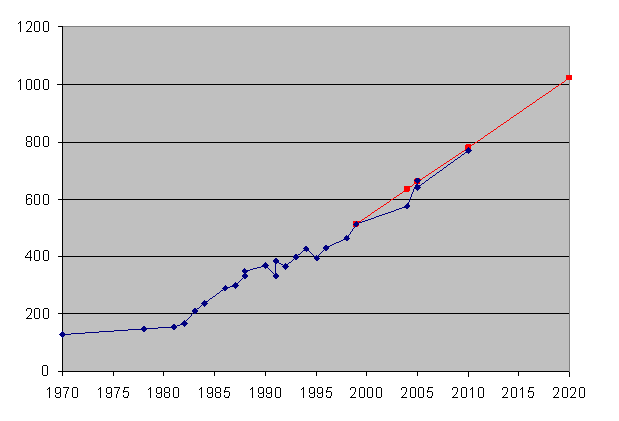
\includegraphics[scale=0.64, clip, viewport=-20 0 680 520]
                 {figures/PrognoseRSAFaktorisierungSecorvo.png}
 }
\caption{Comparison of the published factorization records (blue) and of the
predicted development (red) [Source Fox 2001; last addition 2011]}
\label{secorvo-factorization-forecast}
\end{center}
\end{figure}



\clearpage
% ++++++++++++++++++++++++++++++++++++++++++++++++++++++++++++++++++++++++++
%\vspace{4ex}
\begin{ctsquote}
    To let the possible happen, you again and again have to try the impossible.
\caption[Hermann Hesse]{Hermann Hesse\footnotemark}
\end{ctsquote}
\addtocounter{footnote}{0}\footnotetext{%
  Hermann Hesse, German/Swiss writer and Nobel Prize winner, July 2, 1877 $-$ August 9, 1962.}
% ++++++++++++++++++++++++++++++++++++++++++++++++++++++++++++++++++++++++++

\subsection{Status regarding factorization of concrete large numbers}
\label{nt:NoteFactorization} 

An exhaustive overview about the factoring records
\index{Factorization!factoring records} of composed integers using different
methods can be found on the following web pages:
\vspace{-10pt}
\begin{itemize}
\item[]
     \url{http://www.crypto-world.com} \\
     \url{http://www.tutorgig.com/ed/RSA\_number}  ~~ The RSA Factoring Challenge \\
     \url{http://en.wikipedia.org/wiki/Integer_factorization_records}\\
     \url{http://en.wikipedia.org/wiki/RSA_Factoring_Challenge}
\end{itemize}
%\footnote{%
%This site was not quite up-to-date end of May 2005: RSA-200 was missing.}

The current record (as of Nov. 2012) obtained using the GNFS method
(General Number Field Sieve) factorized a general 232 decimal digit into its
both prime factors.

\vskip +10pt
The last records\footnote{%
The 'RSA numbers' are certain large semiprime numbers (i.e., numbers with
exactly two prime factors)\index{Number!semi prime}. 
They were generated and published by the company RSA Security: In the
RSA Factoring Challenge the prime factors for these numbers are sought.\\
See \url{http://www.rsa.com/rsalabs/node.asp?id=2092}.

RSA Labs offers its challenges since the beginning of the 1990th.
The first RSA Factoring Challenge labeled the numbers, from RSA-100 
to RSA-500, according to their number of decimal digits; the second 
RSA Factoring Challenge labeled the numbers according to their number 
of binary digits. Within the second challenge cash prizes were 
offered for successful factorizations of RSA-576 to RSA-2048 (RSA-576, 
RSA-640 etc. using 64 bit steps upwards --- An exception to this is
RSA-617, which was created prior to the change in the numbering scheme).
But the RSA challenges ended ahead of time in 2007, RSA Inc. retracted
the prize.
All till now unsolved RSA challenges of RSA Labs can also be found at
the website of the cipher challenge ``MysteryTwister C3''
(\url{http://www.mysterytwisterc3.org}).
\index{MTC3}\index{Challenge}\index{Cipher challenge}\index{Crypto challenge}

The 'C numbers' originate from the Cunningham project:
\url{http://www.cerias.purdue.edu/homes/ssw/cun/}.
These are factors of Mersenne numbers, which have a very special
form. This  makes it an order of magnitude easier to factor them
as moduli of the same length build for RSA.
                          }
with factorization algorithms for composed numbers are
listed in the table~\ref{factorizationrecords}.

\begin{table}[ht]
\begin{center}
\begin{tabular}{|c|cccc|}
\hline
	& {\bf Decimal digits} & {\bf Binary digits} & {\bf Factored on} & {\bf Factored by} \\
\hline
	&&&& \\
	RSA-768 & 	232 & 768 & Dec 2010 & Thorsten Kleinjung et al. \\
	RSA-200 & 	200 & 663 & May 2005 & Jens Franke et al. \\
	RSA-640\footnotemark & 	193 & 640 & Nov 2005 & Jens Franke et al. \\
	RSA-576 & 	174 & 576 & Dec 2003 & Jens Franke et al. \\
	RSA-160 & 	160 & 530 & Apr 2003 & Jens Franke et al. \\
	RSA-155	&	155 & 512 & Aug 1999 & Herman te Riele et al. \\
	\dots &&&& \\
	C307 & 		307 & 1017 & May 2007 & Jens Franke et al. \\
	C176 & 		176 & 583 & May 2005 & Kazumaro Aoki et al. \\
	C158 & 		158 & 523 & Jan 2002 & Jens Franke et al. \\
\hline
\end{tabular}
\caption{The current factoring records (as of Nov. 2012)}    % Eyecatcher
\label{factorizationrecords}
\end{center}
\end{table} 
\footnotetext{%
A research group of the GISA solved this challenge which was awarded with
20,000 US dollar using the GNFS method. The researchers needed about five
months to divide this number into its both 320 bit long prime factors.

The researchers around Professor Jens Franke (from the University 
of Bonn, the GISA and the CWI) do not aim on getting cash prizes 
but in extending the research limits. So statements about the 
necessary length of a secure RSA modulus are more well-founded.

See \url{http://www.heise.de/newsticker/meldung/print/65957}.
}


Experiences about the ellipsed time of factorization\index{factorization}
with the open source software Pari-GP, Sage, CrypTool 1 and CrypTool 2)
can be found in ``Zeitexperimente zur Faktorisierung''.\footnote{%
R.-H. Schulz und H. Witten: ``Zeitexperimente zur Faktorisierung''. Ein Beitrag
zur Didaktik der Kryptographie'', in LogIn Heft Nr. 166/167 (2010) 113-120,
(available currently only in German)\\
\url{http://bscw.schule.de/pub/bscw.cgi/d864899/Schulz_Witten_Zeit-Experimente.pdf}
}


\vskip +20pt
%\noindent
Below these last records listed in table~\ref{factorizationrecords} are
explained in more detail\footnote{%
The two methods, GNFS and SNFS, used to do so are shortly illustrated at the 
following web pages:
\index{General Number Field Sieve (GNFS)}
\index{Special Number Field Sieve (SNFS)}
\begin{itemize}
\item[]
      \url{http://en.wikipedia.org/wiki/Special_number_field_sieve} \\
      \url{http://en.wikipedia.org/wiki/General_number_field_sieve}
\end{itemize}
\vspace{-10pt}
}:


% --------------------------------------------------------------------------
%\vskip +20pt
\paragraph*{RSA-155} \label{RSA-155} \index{RSA-155}\mbox{}

On August 22, 1999 researchers from the Netherlands found the solution of this
RSA challenge. They factorized a 155-digit number into its both 78-digit primes
(see chapter~\ref{chptSecurityParam}). 

This 512 bit RSA-155 meant to reach a kind of {\em magic} border.


% --------------------------------------------------------------------------
\vskip +20pt
\paragraph*{C158} \label{C158} \index{C158}\mbox{}
\hypertarget{C158-chap3}{}

On January 18, 2002 researchers at the German University of Bonn\footnote{%
\url{http://www.ercim.org/publication/Ercim\_News/enw49/franke.html}
}
factorized a 158-digit decimal number into its both prime factors (these are
build with 73 and 86 decimal digits) using the GNFS method (General Number
Field Sieve)\index{General Number Field Sieve (GNFS)}.

This record got much less attention within the press than the solution of
RSA-155.

The task of the researchers from Bonn was not initiated by a challenge, but
they wanted to find the last prime factors of the integer $2^{953} - 1$
(see ``Wanted List'' of the Cunningham Project\index{Cunningham project}\footnote{%
Cunningham project: \url{http://www.cerias.purdue.edu/homes/ssw/cun/}}).

The 6 smaller prime factors, already found before have been:
$$
\begin{array}{c}
3, 1907, 425796183929, \\
1624700279478894385598779655842584377, \\
3802306738549441324432139091271828121 \quad {\rm and} \\
128064886830166671444802576129115872060027.
\end{array}
$$
The first 3 factors can be easily computed\footnote{%
E.g.\ using CT1\index{CrypTool 1} via menu 
{\bf Indiv. Procedures \textbackslash{} RSA Cryptosystem \textbackslash{} 
Factorization of a Number}. \\
CT1 can factorize in a reasonable time numbers no longer than 250 bit (Numbers
bigger than 1024 bits are not accepted by CT1). CT2 is able to factorize
numbers bigger than 250 bit length.
}.
The next three prime factors were found by P.~Zimmerman\footnote{%
\url{http://www.loria.fr/~zimmerma/ecmnet}}, 
T.~Grandlund\footnote{\url{http://www.swox.se/gmp/}}
and R. Harley during the years 1999 and 2000 using the elliptic curve
factorization method.

The last remaining factor, called ``C158'', was known to be composite by
then, but its factors were not known (the following 3 lines contain one number):
$$
\begin{array}{c}
39505874583265144526419767800614481996020776460304936 \\
45413937605157935562652945068360972784246821953509354 \\
4305870490251995655335710209799226484977949442955603
\end{array}
$$
The factorization of C158 resulted in the following two 73- and 86-digit prime factors:
$$
\begin{array}{c}
3388495837466721394368393204672181522815830368604993048084925840555281177
\end{array}
$$
and
$$
\begin{array}{c}
1165882340667125990314837655838327081813101 \\
2258146392600439520994131344334162924536139.
\end{array}
$$
So now all 8 prime factors of $2^{953} - 1$ have been found.

\noindent\begin{minipage}{\textwidth}
\vspace{3ex}
Links:
\vspace{-10pt}
\begin{itemize}
\item[]   \url{http://www.loria.fr/~zimmerma/records/gnfs158}\\
          \url{http://www.crypto-world.com/FactorRecords.html}\\
          \url{http://www.crypto-world.com/announcements/c158.txt}
\end{itemize}
\end{minipage}
\vspace{12pt}



% --------------------------------------------------------------------------
\vskip +20pt
\paragraph*{RSA-160} \label{RSA-160} \index{RSA-160}\mbox{}
\hypertarget{RSA-160-chap3}{}

On January 18, 2002 researchers at the German University of Bonn\footnote{%
          \url{http://www.loria.fr/~zimmerma/records/rsa160} \\
          \url{http://www.loria.fr/~zimmerma/records/factor.html} \\
          \url{http://www.crypto-world.com/FactorWorld.html}
} 
factorized a 160-digit number into its both prime factors (these are build
with each 80 decimal digits) using the GNFS method (General Number Field
Sieve)\index{General Number Field Sieve (GNFS)}.

The  computations for the factorization of RSA-160 also took place at the 
German Information Security Agency (GISA) in Bonn.\footnote{%
Every year the GISA\index{GISA} creates a paper to describe which 
crypto algorithms are feasible to generate digital signatures according
to the German signature law -- under participation of experts from
economy and science. To review signature methods based on the
factorization problem the GISA also co-operates with researchers from the
University of Bonn.
Further information about crypto algorithms can be found on the web page of GISA:
   \url{http://www.bsi.bund.de/esig/basics/techbas/krypto/index.htm}
}

The 160-digit decimal number origins from the old challenge list of RSADSI.
This number was retracted after RSA-155 (RSA512) had been factorized 
successfully. The prime factors of RSA-160 were still unknown.
So this record of the team of Prof.\ Franke provides the solution of 
the old challenge, for which RSADSI didn't award a price anymore.

The composite number called ``RSA-160'' is (the following 3 lines contain
one number):
$$
\begin{array}{c}
215274110271888970189601520131282542925777358884567598017049 \\
767677813314521885913567301105977349105960249790711158521430 \\
2079314665202840140619946994927570407753
\end{array}
$$
The factorization of RSA-160 resulted in the following two prime factors:
$$
\begin{array}{c}
p = 45427892858481394071686190649738831 \\         
    656137145778469793250959984709250004157335359
\end{array}
$$
and
$$
\begin{array}{c}
q = 47388090603832016196633832303788951 \\
    973268922921040957944741354648812028493909367
\end{array}
$$

The calculations took place between December 2002 and April 2003.
% \vspace{12pt}
\vspace{24pt}



% --------------------------------------------------------------------------
\vskip +20pt
\hypertarget{RSA-200-chap3}{}
\paragraph*{RSA-200} \label{RSA-200} \index{RSA-200}\mbox{}

On May 9, 2005 the research group of Prof. Jens Franke at the German
University of Bonn\footnote{%
   \url{http://www.loria.fr/~zimmerma/records/rsa200}} announced,
that they achieved to factorize a 200-digit number into its both prime factors 
(these are build with each 100 decimal digits) using the GNFS method 
(General Number Field Sieve)\index{General Number Field Sieve (GNFS)}.

The composite number called ``RSA-200'' is (the following 3 lines contain
one number):
$$
\begin{array}{c}
2799783391122132787082946763872260162107044678695542853756000992932 \\
6128400107609345671052955360856061822351910951365788637105954482006 \\
576775098580557613579098734950144178863178946295187237869221823983
\end{array}
$$
The factorization of RSA-200 resulted in the following two prime factors:
$$
\begin{array}{c}
p = 35324619344027701212726049781984643686711974001976 \\         
    25023649303468776121253679423200058547956528088349
\end{array}
$$
and
$$
\begin{array}{c}
q = 79258699544783330333470858414800596877379758573642 \\
    19960734330341455767872818152135381409304740185467
\end{array}
$$

The calculations took place between December 2003 and May 2005.
The factorization done by the group around Bahr, B\"ohm, Franke, Kleinjung, 
Montgomery and te Riele lasted almost 17 months.
The operating expense of the calculations was about 120,000 
MIPS-years\footnote{%
A MIPS-year (MY) is the quantity of operations a machine can perform in one year,
if the machine constantly achieves one million integer operations per second (MIPS).
For illustration: a INTEL Pentium 100 processor achieves about 50 MIPS.
To factorize a 2048 bit module it is estimated to need about {$8.5 \cdot
 10^{40}$ MY}. }.
\vspace{24pt}



% --------------------------------------------------------------------------
\vskip +20pt
\hypertarget{RSA-768-chap3}{}
\paragraph*{RSA-768} \label{RSA-768} \index{RSA-768}\mbox{}

On December 12, 2009 the research group around Prof. Thorsten
Kleinjung\footnote{%
   \url{http://eprint.iacr.org/2010/006.pdf} \cite{nt:Kleinjung2010}
         } announced,
that they achieved to factorize a 232-digit number into its both prime factors 
(both factors have 116 decimal digits). They used the GNFS method 
(General Number Field Sieve)\index{General Number Field Sieve (GNFS)} in a
way where they did ``oversieving'' on several hundred computers
before starting the matrix step.

The composite number called ``RSA-768'' is (the following 3 lines contain
one number):
$$
\begin{array}{c}
123018668453011775513049495838496272077285356959533479219732245215172640050726\\
365751874520219978646938995647494277406384592519255732630345373154826850791702\\
6122142913461670429214311602221240479274737794080665351419597459856902143413
\end{array}
$$
The factorization of RSA-768 resulted in the following two prime factors (each with 384 bit):
$$
\begin{array}{c}
p = 3347807169895689878604416984821269081770479498371376856891\\
    2431388982883793878002287614711652531743087737814467999489
\end{array}
$$
and
$$
\begin{array}{c}
q = 3674604366679959042824463379962795263227915816434308764267\\
    6032283815739666511279233373417143396810270092798736308917
\end{array}
$$

The calculations took about 2 1/2 years.\footnote{%
This was an ``academic effort'' -- organisations with bigger resources
could do it much faster.}
\vspace{24pt}





% --------------------------------------------------------------------------
\vskip +20pt
\paragraph*{C307 / M1039} \label{C307} \index{C307} \index{M1039}\mbox{}
\hypertarget{C307-chap3}{}

In May 2007 Prof. Franke, Prof. Kleinjung (University of Bonn),
the Japanese telecommunication company NTT and Prof. Arjen Lenstra
(Polytechnical University of Lausanne) announced, that they managed to
factorize a $307$ digit decimal number into its both prime factors
with the SNFS method (Special Number Field Sieve)
\index{Special Number Field Sieve (SNFS)} within 11 months
(the two factors have 80 and 227 decimal digits).

The task of the researchers was not initiated by a challenge, but
they wanted to find the last prime factors of the Mersenne number $2^{1039}+1$
(see ``Wanted List'' of the Cunningham Project\index{Cunningham project}\footnote{%
Cunningham project: \url{http://www.cerias.purdue.edu/homes/ssw/cun/}\\
Cunningham table: \url{http://homes.cerias.purdue.edu/~ssw/cun/pmain1206}\\
The numbers in the Cunningham table have the following syntax:\\
``(2,n)-'' means $2^{n}-1$;~~~
``(2,n)+'' means $2^{n}+1$.\\
To describe the magnitude one writes $p<n>$ or $c<n>$: 
``n'' is the number of decimal digits and ``p'' and ``c'' tell,
whether the number is prime or composite.\\
$2^{1039}-1 = p7 * c307 = p7 * p80 * p227$ \\
It is explained more precisely at the page of the Cunningham project:\\
``2651+ means $2^{651} + 1$ and the size (c209 means 209 decimal digits)
of the
number which was factored.  Then come the new factor(s), the discoverer and
the method used.  Recently, only the multiple polynomial quadratic sieve
(ppmpqs), the elliptic curve method (ecm) and the number field sieve (nfs)
have been used.  `hmpqs' stands for hypercube multiple polynomial quadratic
sieve.  Under `new factors', `p90' means a 90-digit prime and `c201' is a
201-digit composite number.''.
}).\\


The number $2^{1039}-1$ consists of 3 prime factors: The smallest one, 
$p7 = 5080711$ was already known.\footnote{%
This one can also be found using CT1\index{CrypTool 1}  via menu 
{\bf Indiv. Procedures \textbackslash{} RSA Cryptosystem \textbackslash{} 
Factorization of a Number} --- with the algorithms of Brent, Williams or
Lenstra, which are ``relatively'' good to separate small factors.}


To complete this the second factor (co-divider) ``C307'' had to be factorized:
Till then it was only known, that the last remaining factor was composite,
but it was unknown, how many prime factors it had and what are the prime factors.
The following 5 lines contain one number:
$$
\begin{array}{c}
C307 =1159420574072573064369807148876894640753899791702017724986868353538\\
8224838599667566080006095408005179472053993261230204874402860435302\\
8619141014409345351233471273967988850226307575280937916602855510550\\
0425810771176177610094137970787973806187008437777186828680889844712\\
822002935201806074755451541370711023817
\end{array}
$$
The factorization of C307 resulted in the following two 80- and 2276-digit prime factors:
$$
\begin{array}{c}
p80 = 558536666199362912607492046583159449686465270184\\
      88637648010052346319853288374753
\end{array}
$$
and
$$
\begin{array}{c}
p227 = 207581819464423827645704813703594695162939708007395209881208\\
       387037927290903246793823431438841448348825340533447691122230\\
       281583276965253760914101891052419938993341097116243589620659\\
       72167481161749004803659735573409253205425523689
.
\end{array}
$$
So now the number $2^{1039}-1$ is completely factorized in its 3 prime factors.

\noindent\begin{minipage}{\textwidth}
\vspace{3ex}
Links:
\vspace{-10pt}
\begin{itemize}
\item[]]   \url{http://www.loria.fr/~zimmerma/records/21039-}\\
          \url{http://www.crypto-world.com/announcements/m1039.txt}\\
          \url{http://www.crypto-world.com/FactorAnnouncements.html}\\
          \url{http://www1.uni-bonn.de/pressDB/jsp/pressemitteilungsdetails.jsp?detailjahr=2007&detail=160}
\end{itemize}
\end{minipage}






% --------------------------------------------------------------------------
\vskip +70pt
\paragraph*{Size of factorized numbers compared to primality proven numbers}
\mbox{}

As you notice the factorized compound numbers built of 2 prime factors are
much smaller than the especially structured numbers, for which primality 
tests\index{Primality testing} are able to decide whether these numbers are prime 
or not (see chapters~\ref{search_for_very_big_primes},~\ref{primality_tests}
and \ref{spezialzahlentypen}). 

% be_2005_UPDATEN_if-new-mersenne-prime-appears % Eyecatcher_neue-Mersenne
Length of the current world records in decimal notation:

$$ [RSA{-}768~number] ~~\longleftrightarrow{}~~ [47th ~known~Mersenne~prime] $$
$$ 232 ~~ \longleftrightarrow{} ~~ 17,425,170 ~~~~~$$
$$ [see~table~\ref{factorizationrecords}] ~~\longleftrightarrow{}~~ [see~table~\ref{L_n_Largest_Known-Primes}] ~~~~~~~~~~~~~~~~$$



% --------------------------------------------------------------------------
\vskip +60pt
\subsection{Further current research about primes and factorization}
\label{FactorizationResearch}
Prime numbers are part of very many topical research areas in number theory
and computer science. Progress made with factorization is bigger than was
estimated 5 years ago -- this is not only due to faster computers but
also new mathematical knowledge.

The security of the RSA algorithm is based on the empirical observation
that factoring large numbers is a hard problem. A module $n$ (typically,
1024 bit) can be easily constructed as the product of two large primes $p$,
$q$ (typically, 500$-$600 bit each), by calculating $n=pq$. However, it is
a hard problem to extract $p$, $q$ from $n$.  Without knowing $p$ or $q$,
the private key cannot be calculated.

Thus, any progress in efficiency of factorizing large integers will effect the
security of the RSA. As a consequence, the underlying primes $p$, $q$ and,
thus, the module n (1024 bit as of today) have to be increased. In case of a
quantum leap in factorization, the RSA algorithm might be compromised.


% --------------------------------------------------------------------------
\vskip +20pt
%\paragraph*
\subsubsection{Bernstein's paper and its implication on the
               security of the RSA algorithm}
\label{RSABernstein} \index{Factorization!factorization problem}\mbox{}
In his paper ``Circuits for integer factorization: a proposal'' 
(\url{http://cr.yp.to/djb.html}, published November 2001,
D.~J.\ Bernstein \cite{nt:Bernstein2001} addresses the problem of
factorizing large integers. Therefore, his results are of relevance from a
RSA point of view.  As a main result Bernstein claims that the
implementation of the General Number Field Sieve algorithm (GNFS)
 \index{General Number Field Sieve (GNFS)} can be improved to factor, with
the same effort as before, integers with three times more digits.

We note that the definition of \emph{effort} is a crucial point: Bernstein
claims that effort is the product of time and costs of the machine
(including the memory used). The gist of the paper lies in the fact that he
can reduce a big part of factorizing to sorting. Using Schimmler's scheme,
sorting can be optimized by massive parallel computing.  At the end of
section 3 Bernstein explains this effect: The costs of $m^2$ parallel
computers with a constant amount of memory is a constant times $m^2$.  The
costs of a computer with a single processor and memory of size $m^2$ is
also of the order of $m^2$, but with a different constant factor.  With
$m^2$ processors in parallel, sorting of $m^2$ numbers (with Schimmler's
scheme) can be achieved in time $m$, while a $m^2$-memory computer needs
time of the order of $m^2$. Decreasing memory and increasing the number of
processors, the computing time can be reduced by a factor $1/m$ without
additional effort in terms of total costs.  In section 5 it is said that
massive parallel computing can also increase efficiency of factorizing
using Lenstra's elliptic-curve-method (a search algorithm has costs that
increase in a quadratic square manner instead of cubically).

We note that all results achieved so far are asymptotic results. This means
that they only hold in the limit n to infinity. Unfortunately, there is no
upper limit for the residual error (i.e. the difference between the real
and the asymptotic value) for finite n --- a problem which has already been
addressed by the author. As a consequence, one cannot conclude whether the
costs (in the sense of Bernstein) for factorizing 1024$-$2048-bit RSA modules
can be significantly reduced.

There is no doubt that Bernstein's approach is innovative. However, the
reduction of computing time under constant costs comes along with a massive
use of parallel computing --- a scenario which seems not to be realistic
yet. For example, formally 1 sec computing time on one machine and
1/1,000,000 sec time parallel computing time on 1,000,000 machines might
have same costs.  In reality, it is much harder to realize the second
situation, and Bernstein does not take into account the fixed costs, in
particular for building a network between all these computers.

Although distributed computing over a large network might help to overcome
this problem, realistic costs for data transfer have to be taken into
account --- a point which was not addressed in Bernstein's proposal.

As long as there is neither (low cost) hardware nor a distributed computing
approach (based on Bernstein's ideas), there should not be a problem for
RSA. It has to be clarified from which magnitude of n on Bernstein's method
could lead to a significant improvement (in the sense of the asymptotic
result). 

Arjen Lenstra, Adi Shamir et. al. analyzed the paper of Bernstein
\cite{nt:Lenstra2002}.  In summary they expect a factorization improvement on
how much longer the bit length of the keys could be with a factor of 1.17
(instead of factor 3 as proposed by Bernstein).

The abstract of their paper ``Analysis of Bernstein's Factorization
Circuit'' says:

``... Bernstein proposed a circuit-based implementation of the matrix
step of the number field sieve factorization algorithm. We show that under
the non-standard cost function used in [1], these circuits indeed offer an
asymptotic improvement over other methods but to a lesser degree than
previously claimed: for a given cost, the new method can factor integers
that are 1.17 times larger (rather than 3.01).  We also propose an improved
circuit design based on a new mesh routing algorithm, and show that for
factorization of 1024-bit integers the matrix step can, under an optimistic
assumption about the matrix size, be completed within a day by a device
that costs a few thousand dollars.  We conclude that from a practical
standpoint, the security of RSA relies exclusively on the hardness of the
relation collection step of the number field sieve.''

RSA Security\footnote{\url{http://www.rsasecurity.com/}} concludes in its
analysis of the Bernstein paper \cite{nt:RSA Security 2002} from April, 8 2002
also -- as expected -- that RSA is still not compromised.

This is still an ongoing discussion.

When this section was written (June 2002) nothing was publicly known about, how
far there exist implementations of his theoretical onsets and how much
financing there was for his research project.

\vskip +12pt
\noindent\begin{minipage}{\textwidth}
Links:
\vspace{-10pt}
\begin{itemize}
  \item[] \url{http://cr.yp.to/djb.html}\\
          \url{http://www.counterpane.com/crypto-gram-0203.html\#6} \\
          \url{http://www.math.uic.edu}
\end{itemize}
\end{minipage}


% --------------------------------------------------------------------------
\vskip +20pt
%\paragraph*
\subsubsection{The TWIRL device} \label{TWIRLDevice} \index{TWIRL device}
%\mbox{}

In January 2003 Adi Shamir and Eran Tromer from the Weizmann Institute of Science published a preliminary draft called {\em ``Factoring Large Numbers with the TWIRL Device''} raising concerns about the security of key sizes till 1024 bits \cite{nt:Shamir2003}. 

Their abstract summarizes their results very well: ``The security of the RSA
cryptosystem depends on the difficulty in factoring large integers. The best
current factoring algorithm is the Number Field Sieve (NFS), and its most
difficult part is the sieving step. In 1999 a large distributed computation
involving thousands of workstations working for many months managed to factor a
512-bit RSA key, but 1024-bit keys were believed to be safe for the next 15-20
years. In this paper we describe a new hardware implementation of the NFS
sieving step ... which is 3-4 orders of magnitude more cost effective than the
best previously published designs ... . Based on a detailed analysis of all the
critical components (but without an actual implementation), we believe that the
NFS sieving step for 1024-bit RSA keys can be completed in less than a year with
a \$10M device, and that the NFS sieving step for 512-bit RSA keys can be
completed in less than ten minutes with a \$10K device. Coupled with recent
results about the difficulty of the NFS matrix step ... this raises some
concerns about the security of these key sizes.''

A detailed explanation from these two authors also can be found in the
RSA Laboratories CryptoBytes \cite{nt:Shamir2003a}.

The 3-page article in the DuD issue of June 2003 \cite{nt:Weis2003} contains
a very good explanation, how the attack using the Generalized Number Field
Sieve (GNFS) \index{General Number Field Sieve (GNFS)} works and which 
progress is made, to factorize numbers.
At GNFS we can distinguish 2 general steps: 
The sieve step (relation collecting) and the matrix reduction.
Besides the sieve step is highly parallelizable, it dominates the overall
calculation burden. Shamir and Tromer haven't built a TWIRL device yet,
but the estimated costs of 10 till 50 million Euro (in order to factorize
a 1024-bit number) is not prohibitive for secret agencies or big criminal
organizations, because the ``costs for a single espionage satellite is
estimated e.g.\ to be several billion USD''. The authors therefore
recommend, to get as soon as possible rid of today used sensible RSA, 
Diffie-Hellman or ElGamal keys up to 1024 bit and to use then keys of at
least 2048 bit length.
The planned TCPA/Palladium hardware \index{Palladium} will use 2048-bit
RSA keys!

So recommendations like the ones from the GISA (German Information Security Agency) to use higher key lengths are very valid.


% --------------------------------------------------------------------------
\vskip +20pt
%\paragraph*
\subsubsection{``Primes in P'': Primality testing is polynomial}
\label{PrimesinP} \index{Primality testing}%\mbox{}

In August 2002 the three Indian researchers M. Agrawal, N. Kayal and N. Saxena published the paper {\em ``PRIMES in P''} about a new primality testing algorithm called AKS\index{AKS} \cite{nt:Agrawal2002}. 
They discovered a polynomial\index{Polynomial} time deterministic algorithm for determining if a number is prime or not.

The importance of this discovery is that it provides number theorists with new insights and opportunities for further research. Lots of people over centuries have been looking for a polynomial time test for primality, and this result is a major theoretic breakthrough. It shows that new results can be generated from already known facts.

But even its authors note that other known algorithms may be faster (for example ECPP). The new algorithm works on any integer. For example the GIMPS project uses the Lucas-Lehmer primality test which takes advantage of the special properties of Mersenne numbers. This makes the Lucas-Lehmer test much faster, allowing to test numbers with millions of digits while general purpose algorithms are limited to numbers with a few thousand digits.

\noindent Current research results on this topic can be found at:
\vspace{-10pt}
\begin{itemize}
  \item[] \url{http://www.mersenne.org/} \\
          \url{http://fatphil.org/maths/AKS/} Original paper in English\\
          \href{http://ls2-www.cs.uni-dortmund.de/lehre/winter200203/kt/material/primes.ps}{\tt http://ls2-www.cs.uni-dortmund.de/lehre/winter200203/kt/material/primes.ps} \\% \url... created overfull \hbox
	  \hspace*{2em}Good explanation in German by Thomas Hofmeister.
\end{itemize}
\vskip +10 pt


% --------------------------------------------------------------------------
% \vskip +20pt
\newpage
\subsubsection{Shared Primes: Modules with common prime factors}
\label{nt_Shared-Primes} \index{Prime!Shared}%\mbox{}
%~\ref{nt_Shared-Primes}, page~\pageref{nt_Shared-Primes}

The RSA algorithm for public-key cryptography is based on the presumed difficulty of factoring large bi-prime integers, the factoring problem. However, as pointed out in Lenstra et al \cite{nt:Lenstra2012} it is possible, given a set of moduli, to factor some of them by finding shared primes. This way the factoring problem is bypassed using a simple greatest common divisor (gcd) operation. It is no trivial task to extract common shared primes and to factor the according moduli efficiently for a very big number of given moduli (several millions).

Using the gcd only works if the RSA keys were not generated randomly. Taking into consideration the significance of strong cryptographic keys it is important to verify that all keys were generated following the principle of true randomness \cite{nt:Esslinger2012}. 

When Lenstra et al published their paper \cite{nt:Lenstra2012} in Feb. 2012, they did not publish the source code. However, soon afterwards the source code of a similar program was published at the CrypTool website\footnote{%
\url{http://www.cryptool.org/en/ctp-dokumentation-en/361-ctp-paper-rsa-moduli}
%\url{http://www.cryptool.org/de/ctp-dokumentation-de/361-ctp-paper-rsa-moduli}
}
in Python and C++, and at the page used by \cite{nt:Heninger2012}\footnote{\url{https://www.factorable.net/}
}.
The fastest code known to me comes with \cite{nt:Heninger2012}.

These applications find all shared factors that may exist, given a finite set of moduli -- even if this set includes millions of moduli. Such an application enables system administrators to test their own RSA keys. 

The quite naive way to find all shared factors would be to compare each modul with all other moduli which has a complexity growing quadratically with the number of moduli.
A very efficient method using trees for comparing all gcd pairs is based on a publication of Dan Bernstein in 2005 \cite{nt:Bernstein2005}. Bernstein uses a precalculation which leads to the product of all moduli. It's another example showing how helpful precalculations can be to break cryptographic systems (another famous example are rainbow tables used to find the origin of a hash value \cite{nt:Oechslin2003}).


The following Sage sample shows the very different run times when calculating a gcd and a factorization. The section after this sample will explain the essential part of the method used in \cite{nt:Heninger2012}: Using the trees accelerates the calculation of the gcd pairs a lot.

The Sage sample~\ref{nt_sagesample_Compare-Runtime-gcd-factoring} shows that multiplication of factors, dividing a modul with a known factor, or calculating the gcd is very fast. However, factoring moduli steeply increases with longer moduli. Even the relatively small moduli used in this example show this: The smaller modul (69 decimal digits, 228 bits) took 76 seconds, while the bigger one (72 decimal digits, 239 bits) took almost 217 seconds.

In addition, the operations multiplication, divsion and gcd show big differences in runtime when the used operands are very different in size.

% Just to show the origin of the used primes
% sage: factor (2^211-1)
% 15193 * 60272956433838849161 * 3593875704495823757388199894268773153439
%
% sage: factor (2^214-1)
% 3 * 643 * 84115747449047881488635567801 * 162259276829213363391578010288127
\begin{sagecode}
\begin{Verbatim}%
[fontsize=\footnotesize,fontshape=tt]

# Multiplication
sage: 3593875704495823757388199894268773153439 * 84115747449047881488635567801
302301541122639745170382530168903859625492057067780948293331060817639

sage: 3593875704495823757388199894268773153439 * 162259276829213363391578010288127
583139672825572068433667900695808357466165186436234672858047078770918753


# Division
sage: time 302301541122639745170382530168903859625492057067780948293331060817639 / 
           3593875704495823757388199894268773153439
Wall time: 0.00 s
84115747449047881488635567801

sage: time 583139672825572068433667900695808357466165186436234672858047078770918753 / 
           3593875704495823757388199894268773153439
Wall time: 0.00 s
162259276829213363391578010288127


# Calculate gcd
sage: time gcd (583139672825572068433667900695808357466165186436234672858047078770918753,
                302301541122639745170382530168903859625492057067780948293331060817639)
Wall time: 0.00 s
3593875704495823757388199894268773153439


# Factorize
sage: time factor (583139672825572068433667900695808357466165186436234672858047078770918753)
Wall time: 217.08 s
162259276829213363391578010288127 * 3593875704495823757388199894268773153439

sage: time factor (302301541122639745170382530168903859625492057067780948293331060817639)
Wall time: 76.85 s
84115747449047881488635567801 * 3593875704495823757388199894268773153439

\end{Verbatim}
\caption{Comparing the runtime of calculating a gcd and performing a factorization}
\label{nt_sagesample_Compare-Runtime-gcd-factoring}
\end{sagecode}



\clearpage
\section*{Efficient computing of all gcd pairs and explanation of the formula used}

The paper "Mining Your Ps and Qs: Detection of Widespread Weak Keys in Network Devices"~\cite{nt:Heninger2012} explains the algorithm how the gcd's of every pair of RSA moduli are calculated efficiently.

First the product $P$ of all moduli $m_{i}$ is calculated using a product tree. Then a remainder tree is build modulo the squares of the moduli. Then the gcd's of a defined modul $m_{i}$ and of the remainders $z_{i}$ divided by this defined modul are calculated. 

This is visualized in Figure \ref{Figure_Bernstein_Computing-all-pairs-GCDs} which is a copy from \cite{nt:Heninger2012} (where the moduli are called $N_{i}$
instead of $m_{i}$:
\begin{figure}[ht]
\begin{center}
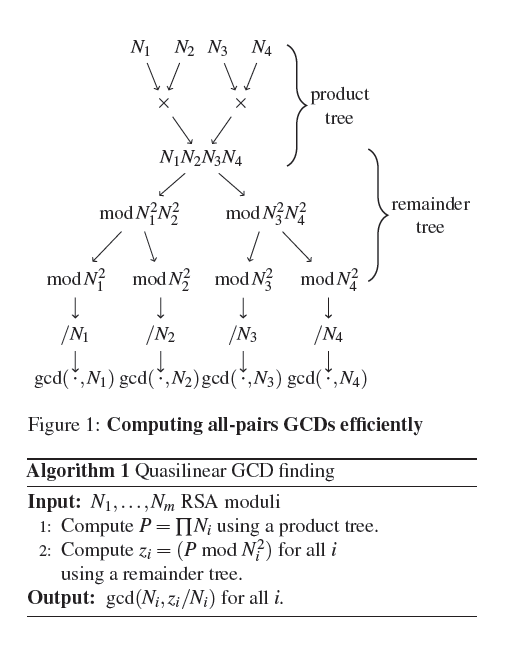
\includegraphics[scale=0.7]{figures/Bernstein_Computing-all-pairs-GCDs.png}
\caption{Algorithm and Figure to compute all gcd pairs efficiently} 
\label{Figure_Bernstein_Computing-all-pairs-GCDs}
\end{center}
\end{figure}


The paper~\cite{nt:Heninger2012} explains well \textit{how} the algorithm works, but not as well \textit{why}. The product $P$ of all moduli is a very big number, even compared to a single modul. Without the simplifications from the remainder tree you would go the following way: Calculate $gcd_{i} = gcd( P / m_{i},  m_{i}) $ for all i. Compare each $gcd_{i} \ne 1$ with all other $gcd_{j} \ne 1$ with  $j \ne i$. If two gcd's are the same, then their moduli share a factor.

As it's very slow to calculate this for numbers with such a big difference in size, the remainder tree is used. Despite it seems to consist of more steps it's a huge simplification.

Within the remainder tree you get -- at the end -- $(P \bmod ({m_{i}^{2}}) ) / m_{i}$ for all $i$.\footnote{%
It would not make sense to calculate $(P \bmod m_{i} ) / m_{i}$
as $(P \bmod m_{i} )$ is always $= 0$.

Sample with very small moduli:\\
$ m_{1} = 2*3 = 6;~~~ m_{2} = 2*7 = 14;~~~ P=6*14=84 $\\
$ P \bmod m_{1} = 84 \bmod 6 = 0;~~~ P \bmod {m_{1}^{2}} = 84 \bmod 36 = 12 $\\
$ P \bmod m_{2} = 84 \bmod 14 = 0;~~~ P \bmod {m_{2}^{2}} = 84 \bmod 196 = 84 $\\
$gcd_{1} = gcd(12/6, 6) = gcd(2, 6) = 2 $\\
$gcd_{2} = gcd(84/14, 14) = gcd(6, 14) = 2 $

The way the tree is structured it also would not make sense to first divide and then do the modulo calculation, as making the division first would lead just to the given moduli but in reversed order.

It also would not make sense to calculate $(P \bmod ({m_{i}^{3}}) ) / {m_{i}^{2}})$ as this is only additional effort with no improvement.
}

The main remaining question now is: Why does $gcd((P \bmod {m_{i}^{2}})/ m_{i}, m_{i})$ deliver the same result as $gcd( P / m_{i}, m_{i})$ ?
We prove that this identity is correct.

P represents here the product of all moduli, and $m_{i}$ represents any
arbitrary modulus.%\mbox{}\\\mbox{}\\

$$gcd((P \bmod {m_{i}^{2}})/ m_{i}, m_{i})~~~  \overset{!}{=}  ~~~gcd( P / m_{i}, m_{i})$$
$ \Longleftrightarrow $~~~\footnote{According to Euklid's algorithm the following identities are true:
\mbox{}\\
$gcd((P \bmod {m_{i}^{2}})/ m_{i}, m_{i})=gcd((P \bmod {m_{i}^{2}})/ m_{i} \bmod{m_{i}}, m_{i})$ \mbox{}\\
$gcd( P / m_{i}, m_{i})=gcd( P / m_{i} \bmod{m_{i}}, m_{i})$\mbox{}
}

$$gcd(((P \bmod {m_{i}^{2}})/ m_{i}) \bmod {m_{i}}, m_{i})~~~  \overset{!}{=}  ~~~gcd( (P / m_{i}) \bmod {m_{i}}, m_{i})$$
$ \Longleftrightarrow $~~~\footnote{The gcd's are equal if both their first arguments are equal.
}

$$((P \bmod {m_{i}^{2}})/ m_{i}) \bmod {m_{i}}~~~  \overset{!}{=}  ~~~ (P / m_{i}) \bmod {m_{i}}$$
$ \Longleftrightarrow $~~~\footnote{The following transformations are all equalities.
}

$$(P \bmod{m_{i}^{2}})/ m_{i} - P / m_{i} \equiv 0   \bmod{m_{i}}~~~ \Leftrightarrow ~~~  m_{i} ~~ | ~~ ((P \bmod{m_{i}^{2}})/ m_{i} - P / m_{i})$$~~~\footnote{%
According to the definition of modulus and division it is:\\
$a \bmod{b} ~~ \Longleftrightarrow ~~ a - b * \lfloor a/b \rfloor$\\
So $P \bmod{m_{i}^{2}}$ can be written as $ P-m_{i}^{2} \lfloor P/m_{i}^{2} \rfloor$.
}

$$ m_{i} ~~ | ~~ ((P-m_{i}^{2}* \lfloor P/m_{i}^{2} \rfloor - P))/m_{i}$$~~~\footnote{%
$P$ reduces itself, the exponent in the $m_{i}$ enumerator is simplified with the  $m_{i}$ denominator.
}

$$ m_{i} ~~ | ~~ (m_{i}* \lfloor P/m_{i}^{2} \rfloor)$$

As this is true, we can conclude that the two gcds are equivalent.

% yyyyyyyyyyyyyyyyyyyyyyyyyyy

% S�tze und Links:
% https://en.wikipedia.org/wiki/Greatest_common_divisor
% https://de.wikipedia.org/wiki/Gr%C3%B6%C3%9Fter_gemeinsamer_Teiler


%TODO: Wohl durch das verschobene Sage-Beispiel wirkt das \newpage vor dem ff. Kapitel nicht!


% ++++++++++++++++++++++++++++++++++++++++++++++++++++++++++++++++++++++++++
% \vskip +40 pt
\newpage
\begin{ctsquote}
It is our choices, that show what we truly are, far more than our abilities.
\caption[Joanne K. Rowling]{Joanne K. Rowling\footnotemark}\index{Rowling, Joanne}
\end{ctsquote}

\addtocounter{footnote}{0}\footnotetext{Joanne K. Rowling, ~``Harry Potter and the Chamber of Secrets'', Bloomsbury, 1998, 
last chapter ``Dobby's reward'', p.~245, by Dumbledore.}

%\begin{quote}
%{\em Joanne K. Rowling}\footnote{Joanne K. Rowling, ~``Harry Potter and the Chamber of Secrets'', Carlsen, 1998, 
%last chapter ``Dobby's reward'', p.~343.}:\\
%It is our choices, that show what we truly are, far more than our abilities.
%\end{quote}

% ++++++++++++++++++++++++++++++++++++++++++++++++++++++++++++++++++++++++++
\section{Applications of asymmetric cryptography using numerical examples}

The results of modular arithmetic are used extensively in \index{Cryptography!modern} modern cryptography. Here we will provide a few examples from 
cryptography using small\footnote{In the RSA procedure, we call numbers ``small'' if the bit lengths are much less than $1024$ bits (i.e. $308$ decimal points). In practice,
$1024$ bits is currently considered the minimum length for a secure RSA modul.} numbers.

Enciphering a text entails applying a function (mathematical operation) to a character string (number) to generate a 
different number. Deciphering entails reversing this function, in other words using the distorted image that the function 
has created from the plaintext in order to restore the original image. For example, the sender could take the plaintext 
$M$ of a confidential message and add a secret number, the key $S$, to obtain the ciphertext $C$:
$$C = M + S.$$
The recipient can reconstruct the plaintext by reversing this operation, in other words by subtracting $S$:
$$M = C - S.$$
Adding $S$ reliably makes the plaintext impossible to read. However, this encryption is rather weak, because all an 
interceptor needs to do to calculate the key is obtain a plaintext and the associated ciphertext
$$S = C - M,$$
and can then read any subsequent messages encrypted using $S$. \\
The essential reason for this is that subtraction is just as simple an operation as addition. 


% --------------------------------------------------------------------------
\hypertarget{OneWayFunktion2}{}%
\subsection{One way functions}\index{One way function}
\label{OneWayFunktion2}%
If the key is to be impossible to determine even with knowledge of both the 
plaintext and the ciphertext, we need a function that is, on the one hand, 
relatively easy to calculate -- we don't want to have problems encrypting 
messages. On the other hand, the inverse function should exist (otherwise 
information would be lost during encryption), but should be de facto 
incalculable.

What are possible candidates for such a {\bf one way function}? We could take multiplication rather than addition, 
but even primary school children know that the inverse function, division, is only slightly more difficult than multiplication 
itself. We need to go one step higher in the hierarchy of calculation methods. It is still relatively simple to calculate the 
power of a number, but the corresponding two reverse functions -- {\em taking roots} (find $b$ in the equation $a = b^c$  when $a$ 
and $c$ are known) and {\em calculating logarithms} (find $c$ in the above equation when $a$ and $b$ are known) are so complicated 
that pupils normally do not learn them at school.

Although a certain structure can still be recognised for addition and multiplication, raising numbers to the power of 
another or calculating exponentials totally mixes up all the numbers. Knowing a few values of the function doesn't tell 
us much about the function as a whole (in contrast to addition and multiplication).


% --------------------------------------------------------------------------
\vskip +10 pt
\subsection{The Diffie-Hellman key exchange protocol}
\index{Diffie, Whitfield} 
\index{Hellman, Martin} 
\index{Key agreement (key exchange)!Diffie-Hellman}
\index{Diffie-Hellman}

Whitfield Diffie, Martin E. Hellman and Ralph Merkle developed this DH key 
exchange protocol in Stanford in 1976.\footnote{%
  With CT1\index{CrypTool 1} this exchange protocol has been
  visualized: You can execute the single steps with concrete numbers using 
  menu {\bf Indiv. Procedures \textbackslash{} Protocols
  \textbackslash{} Diffie-Hellman Demonstration}.\\
  In JCT\index{JCrypTool} you can find it in the default perspective
  via the menu item {\bf Visuals \textbackslash{} Diffie-Hellman
  Key Exchange (EC)}.
}

Alice and Bob\footnote{Bob\index{Bob} and Alice\index{Alice} are the default
names used for the two authorized participants in a protocol (see
\cite[p. 23]{nt:Schneier1996nt}).
} use a one way function to obtain a key $S$, the session key, for subsequent
correspondence. This is then a secret that is only known to the two of them.
Alice selects a random number $a$ and keeps it secret. She applies a one way
function to $a$ to calculate the number $A = g^a$ and sends it to Bob. He does
the same, by selecting a secret random number $b$, calculating $B = g^b$ and
sending it to Alice. The number $g$ is random and can be publicly known.
Alice applies the one way function together with her secret number $a$ to
$B$, while Bob does the same with his secret number $b$ and the received
number $A$.

The result $S$ is the same in each case because the one way function is
commutative: $(g^a)^b = (g^b)^a$. But even Bob cannot reconstruct Alice's
secret number $a$ from the data available to him, while Alice cannot
determine Bob's secret number $b$. And a perpetrator who knows $g$ and
has intercepted both $A$ and $B$ cannot use this knowledge to 
determine $a, b$ or $S$.

\vskip +10 pt
\input{figures/DH-en.latex}
\vskip +20 pt

\noindent {\bf Procedure:}\par  %\par bewirkt Zeilenumbruch
\nopagebreak
\noindent Alice and Bob want to negotiate a secret session key $S$ via
a channel that may be intercepted. 
\begin{itemize}
\item[{\bf 1.}] They select a prime number $p$ and a random number $g$ and exchange this information openly.
\item[{\bf 2.}] Alice now selects $a$, a random number less than $p$ and keeps it secret.

                Similarly, Bob selects $b,$ a random number less than $p$ and keeps it secret.
\item[{\bf 3.}] Alice now calculates $A \equiv g^a {\rm ~(mod~} p)$.\\
                Bob calculates $B \equiv g^b {\rm ~(mod~} p)$.
\item[{\bf 4.}] Alice sends the result $A$ to Bob.\\
                Bob sends the result $B$ to Alice.
\item[{\bf 5.}] In order to now determine the session key to be used by both,
                they both separately raise the respective results they have
                received to the power of their secret random number modulo $p$.
                This means: 
\begin{itemize}
    \item[-] Alice calculates $S \equiv B^a {\rm ~(mod~} p)$ and
    \item[-] Bob calculates $S \equiv A^b {\rm ~(mod~} p)$.
\end{itemize}
\end{itemize}
Even if a spy intercepts $g, p$, and the interim results $A$ and $B$, he cannot
use these in order to determine the used session key used -- due to the
difficulty of calculating the discrete logarithm\footnotemark.
\footnotetext{%
Further details about
the\index{Logarithm problem!discrete}\index{Discrete logarithm}
\hyperlink{HT-Discrete-Logarithm-as-Basis}{discrete logarithm problem}
can be found in chapter~\ref{L-Discrete-Logarithm-as-Basis}.
}

\vskip + 5pt
\noindent We will now use an example with (unrealistically) small numbers to illustrate this.
\vskip +1em

\begin{example}{ using small numbers:}
\begin{itemize}
\item[{\bf 1.}] Alice and Bob select $g = 11, p = 347$.
\item[{\bf 2.}] Alice selects $a = 240$, Bob selects $b = 39$ and they keep $a$ and $b$ secret.
\item[{\bf 3.}] Alice calculates $A \equiv g^a \equiv 11^{240}  \equiv 49 {\rm ~(mod~} 347).$\\
                Bob calculates $B \equiv g^b \equiv 11^{39} \equiv 285 {\rm ~(mod~} 347).$
\item[{\bf 4.}] Alice sends Bob:   $A \equiv 49$,\\
                Bob sends Alice: $B \equiv 285$.
\item[{\bf 5.}] Alice calculates $B^a \equiv 285^{240} \equiv 268 {\rm ~(mod~} 347),$\\
                Bob calculates $A^b \equiv   49^{39} \equiv 268 {\rm ~(mod~} 347).$
\end{itemize}
Alice and Bob can now communicate securely using their shared session key. Even if spies were to intercept everything 
transferred via the connection:
$g = 11, p = 347, A = 49$ and $B = 285$, they would not be able to calculate the secret key.
\end{example}

\newpage
\begin{remark}{:}\\
In this example using such small numbers, it is easily possible to calculate the discrete
logarithms, but with large numbers the discrete logarithm\index{Discrete logarithm}
problem\footnote{%
You can use Sage to determine the discrete logarithm $x$ that solves the
equation $11^x \equiv 49 \pmod{347}$ (here for Alice)\index{Sage}:
\texttt{discrete\_log(mod(49, 347), mod(11, 347))}. The returned value
is $67$.\\
Such number theoretic tasks can also be solved using other
tools like PariGP\index{Pari-GP}, LiDIA\index{LiDIA}, BC\index{BC} or
Mathematica\index{Mathematica}
(see the list of web sites in the appendix at the end of this chapter):\\
- Pari-GP: \texttt{znlog(Mod(49,347),Mod(11,347))}.\\
- LiDIA:   \texttt{dl(11,49,347)}.\\
- Mathematica: The general Solve function delivers the {em tdep message} ``The equations
  appear to involve the variables to be solved for in an essentially non-algebraic way''.\\
- Mathematica: {\tt MultiplicativeOrder[11, 347, 49]}.\\
All deliver the result $67$.
}${}^,$\footnote{%
Why have the functions delivered the value $67$ for the discrete
logarithm\index{Discrete logarithm} of Alice rather than $240$ which Alice
selected as exponent $a$?\\
The discrete logarithm is
the smallest natural exponent that solves the equation 
$11^x \equiv 49 \pmod{347}$. Both $x = 67$ and $x = 240$ (the number
selected in the example) satisfy the equation and can therefore be
used to calculate the session key: 
$285^{240} \equiv 285^{67} \equiv 268 \pmod{347}$.
If Alice and Bob
had selected a primitive root\index{Primitive root} modulo $p$ as base $g$, then for every
remainder from the set $\{1, 2, \dots, p-1 \}$ there is exactly one
exponent from the set $\{0, 1, \dots, p-2 \}$. \\
\indent As an aside, there are $172$ different primitive roots modulo $347$,
$32$ of which are prime (not necessary). Since the number $11$
selected for $g$ in the example is not a primitive root\index{Primitive root} of $347$, the
remainders do not take all values from the set $\{1, 2, \dots, 346 \}$. 
Thus, for a particular remainder there may be more than one exponent
or even no exponent at all in the set $\{0, 1, \dots, 345 \}$ that
satisfies the equation.\\
With the relevant Sage\index{Sage} commands you find:\\
\texttt{is\_prime(347)=True}, \texttt{euler\_phi(347)=346}, \texttt{gcd(11,347)=1} and 
\texttt{multiplicative\_order(mod(11, 347))=173}.

\begin{tabular}{|c|c|l|}
\hline
i  & $11^i \bmod 347$ & \\
\hline
      0  &          1   &  \\
      1  &         11   &  \\                                     
      2  &        121   &  \\                                     
      3  &        290   &  \\                                     
     67  &         49   & searched exponent \\                    
    172  &        284   &  \\                                                  
    173  &          1   &= multiplicative order of $11^i \bmod 347$ \\ 
    174  &         11   &  \\                                                     
    175  &        121   &  \\                                     
    176  &        290   &  \\                                     
    240  &         49   & searched exponent \\
\hline
\end{tabular}
\vskip +6 pt

\noindent Further information can be found in
chapter~\ref{nt:AppArith3a2} ``\nameref{nt:AppArith3a2}''.
}
is extremely difficult to solve.
\end{remark}

\noindent To get the discrete logarithms, here we need to calculate:\\
For Alice: $11 ^ x \equiv 49 {\rm ~(mod~}347)$, that means $\log_{11}(49) {\rm ~(mod~}347).$\\
For Bob: $11 ^ y \equiv 285 {\rm ~(mod~}347)$, that means $\log_{11}(285){\rm ~(mod~}347)$.



% ++++++++++++++++++++++++++++++++++++++++++++++++++++++++++++++++++++++++++
\newpage
\hypertarget{Chapter_ElementaryNT_12}{}
\section[The RSA procedure with actual numbers]{The RSA procedure with actual numbers\footnotemark}
\footnotetext{%
    \index{Sage}%
    \index{Nguyen, Minh Van }%
    Additional material: Minh Van Nguyen, ``Number Theory and the RSA
    Public Key Cryptosystem'', 2009. An introductory tutorial on using
    Sage to study elementary number theory and public key
    cryptography. A didactically very clear article about some basic
    number theory and Sage usage.\\
    \url{http://nguyenminh2.googlepages.com/sage_numtheory-rsa.pdf}.
}
\label{rsaconcrete}\index{RSA}

\begin{ctsquote}
``Games are Nature's way of preparing us to face difficult realities. Are you finally ready to face reality, Sergeant?''
\caption[Daniel Suarez]{Daniel Suarez\footnotemark}\index{Suarez, Daniel}
\end{ctsquote}
\addtocounter{footnote}{0}\footnotetext{Daniel Suarez, ``Daemon'', Dutton Adult, 2010,
Chapter 45, ``Respawning'', p. 610, Sobol.}

Having described above \hyperlink{RSA}{how the RSA procedure works}, we will now work through the steps using actual, but small, numbers.


% --------------------------------------------------------------------------
\subsection{RSA with small prime numbers and with a number as message}

Before applying the RSA procedure to a text, we will first demonstrate it
directly using a single number as message.\footnote{%
   Using CT1\index{CrypTool 1} you can solve this with the menu {\bf Indiv.
   Procedures \textbackslash{} RSA Cryptosystem \textbackslash{} RSA Demonstration}.
}
\begin{itemize}
\item[{\bf 1.}] Let the selected prime numbers be $p=5$ and $q=11$. \\
Thus, $n=55$ and $J(n)=(p-1)*(q-1)=40$.
\item[{\bf 2.}] $e = 7$ ($e$ should\footnote{%
                See footnote~\ref{foot:Selection-of-e} on page
                \pageref{foot:Selection-of-e}.} lie between $11$ and $39$,
                and must be relatively prime to $40$).
\item[{\bf 3.}] $d = 23$ (since $23*7 \equiv 161 \equiv 1{\rm ~(mod~} 40)$),
    \begin{itemize}
    \item[] $\rightarrow$ Public key of the recipient:  $(55, 7),$
    \item[] $\rightarrow$ Private key of the recipient: $(55, 23).$
    \end{itemize}
\item[{\bf 4.}] Let the message be the number $M = 2$ (so no division into blocks is required).
\item[{\bf 5.}] Encryption: $C \equiv 2^7 \equiv 18 {\rm ~(mod~}55).$
\item[{\bf 6.}] The ciphertext is simply the number $C = 18$ (we therefore do not need to divide it into blocks).
\item[{\bf 7.}] Decryption: 
        $M \equiv 18^{23} \equiv 18^{(1+2+4+16)} \equiv 18*49*36*26 \equiv 2 {\rm ~(mod~}55).$
\end{itemize}


We will now apply the RSA procedure to a text, first using the upper case alphabet ($26$ characters), then using the entire ASCII character set as the basis for the messages.


% --------------------------------------------------------------------------
\subsection[RSA with slightly larger primes and an upper-case message]{RSA with slightly larger primes and a text of upper case letters}
\label{rsaex2}

We have the text ``ATTACK AT DAWN'', and the characters are coded according to
table~\ref{alphacode}.\footnote{%
Using CT1\index{CrypTool 1} you can solve this with the menu {\bf Indiv. Procedures
\textbackslash{} RSA Cryptosystem \textbackslash{} RSA Demonstration}.
This is also described in the tutorial/scenario in CT1's online help [Options,
specify alphabet, number system, block length\index{Block length} 2 and decimal
representation].
}

\begin{table}[ht]
\begin{center}
\begin{tabular}{|c|l||c|l|}
\hline
Character & Numerical value & Character & Numerical value \\
\hline
\hline
Blank    & 0   & M  & 13 \\
A        & 1   & N    & 14 \\ 
B        & 2   & O    & 15 \\ 
C        & 3   & P    & 16 \\  
D        & 4   & Q    & 17 \\ 
E        & 5   & R    & 18 \\ 
F        & 6   & S    & 19 \\  
G        & 7   & T    & 20 \\  
H        & 8   & U    & 21 \\ 
I        & 9   & V    & 22 \\   
J       & 10   & W    & 23 \\  
K       & 11   & X    & 24 \\ 
L       & 12   & Y    & 25 \\
&              & Z    & 26 \\
\hline
\end{tabular}
\end{center}
\hypertarget{Grossbuchstaben-Alphabet}{}    
\caption{Capital letters alphabet}\index{Capital letters alphabet}
\label{alphacode}
\end{table}
\vskip +20 pt

\noindent {\bf Key generation (steps 1 to 3)}:\\
{\bf 1.} $p=47, q=79$ $( n= 3713; ~J(n) = (p-1)*(q-1)=3588).$ \\
{\bf 2.} $e = 37$ ($e$ should\footnote{%
                See footnote~\ref{foot:Selection-of-e} on page
                \pageref{foot:Selection-of-e}.} lie between $79$ and $3587$,
                and must be relatively prime to $3588$). \\
{\bf 3.} $d=97$ (since $e*d=1{\rm ~mod~}J(n); 37*97 \equiv 3589
                        \equiv 1{\rm ~(mod~}3588) \;$).\footnote{%
 How to compute $d = 97$ using the {\em extended} gcd algorithm is shown
 in appendix~\ref{nt:NumberTheory_Appendix_GCD}} \\

\noindent {\bf 4. Encryption}:\\
{\tt
\begin{tabular}{rcccccccccccccccccccc}
{\rm Text:} & A & T & T & A & C & K & & A & T &  & D & A & W & N \\
{\rm Number:} & 01 & 20 & 20 & 01 & 03 & 11 & 00 & 01 & 20 & 00 & 04 & 01 & 23 & 14
\end{tabular}
}

\noindent This $28$-digit number is divided into $4$-digit parts
(because $2626$ is still smaller than $n=3713$):\\
{\tt 0120 2001 0311 0001 2000 0401 2314}

\label{SrcArith4a}
\noindent All 7 parts are encrypted using: $C \equiv M^{37}{\rm ~(mod~}3713)$:\footnote{%
  See chapter~\ref{nt:AppArith4a} ``\nameref{nt:AppArith4a}''
  for source code to do RSA encryption using Sage. \\
  You can also encrypt the message with CT1\index{CrypTool 1} via the menu path 
  {\bf Indiv. Procedures \textbackslash{} RSA Cryptosystem \textbackslash{}
  RSA Demonstration}.
} \\
{\tt 1404 2932 3536 0001 3284 2280 2235}

\noindent {\bf 5. Decryption}: \\
Ciphertext: {\tt 1404 2932 3536 0001 3284 2280 2235 }

\noindent This $28$-digit number is divided into $4$-digit parts.

\noindent All 7 parts are decrypted using:  $M \equiv C^{97}{\rm ~(mod~}3713)$: \\
{\tt 0120 2001 0311 0001 2000 0401 2314}

\noindent The 2-digit numbers are transformed into capital letters and blanks.

\noindent Using the selected values it is easy for a cryptanalyst\index{Cryptanalysis}
to derive the secret values from the public 
parameters $n=3713$ and $e=37$ by revealing that $3713 = 47 * 79$.

\noindent If $n$ is a $768$-bit number, there is, according to present knowledge,
little chance of this.


% --------------------------------------------------------------------------
\subsection{RSA with even larger primes and a text made up of ASCII characters}

In real life, the ASCII alphabet is used to code the individual characters
of the message as $8$-bit numbers.

\noindent The idea for this task\footnote{%
Using CT1\index{CrypTool 1} you can solve this via the menu path {\bf Indiv. Procedures
\textbackslash{} RSA Cryptosystem \textbackslash{} RSA Demonstration}.
} 
is taken from the example in \cite[p. 271]{nt:Eckert2003}\index{Eckert 2003}.

\noindent Coded in decimal notation, the text ``RSA works!'' is as follows: \\
{\tt
\begin{tabular}{rcccccccccccccccccccc}
{\rm Text:} & R & S & A &   & w & o & r & k & s & ! \\
{\rm Number:} & 82 & 83 & 65 & 32 & 119 & 111 & 114 & 107 & 115 & 33 
\end{tabular} } % \tt

\noindent We will work through the example in 2 variants. The steps 1 to 3 are common for both.
\par
\noindent {\bf Key generation (steps 1 to 3)}:
\label{SrcArith4b} \\
{\bf 1.} $p=503,~q=509 \quad (n= 256,027; \; J(n)=(p-1)(q-1)=255,016=2^3*127*251)$.\footnote{%
  See chapter~\ref{nt:AppArith4b} ``\nameref{nt:AppArith4b}''
  for the source code to factorize the number $J(n)$ using Sage.
  Using CT1\index{CrypTool 1} you can solve this with the 
  {\bf Indiv. Procedures \textbackslash{} RSA Cryptosystem \textbackslash{} 
  Factorization of a Number}.} \\
{\bf 2.} $e=65,537$ \\
\strut\quad\ ($e$ should\footnote{%
                See footnote~\ref{foot:Selection-of-e} on page
                \pageref{foot:Selection-of-e}.}
                lie between $509$ and $255,015$, and must\footnote{%
       $e$ cannot, therefore, be $2, 127$ or $251$
       ($65,537 = 2^{16}+1$) ($255,016 = 2^{3}*127*251$).\\
       In real life, $J(n)$ is not factorized but rather the Euclidean
       algorithm is used for the selected e to guarantee that
       ${\rm gcd}(e,J(n))=1$.
                 } be relatively prime to $255,016$).\\
{\bf 3.} $d=231,953$ \\
\strut\quad\ (since $e \equiv d^{-1}{\rm ~mod~}J(n): ~65,537*231,953 \equiv 15,201,503,761 \equiv 1
{\rm ~(mod~}255,016)$).\footnote{Other possible combinations of $(e,d)$ include: $(3, 170,011)$, $(5, 204,013)$, $(7, 36,431)$.}


% --------------------------------------------------------------------------
\subsection*{Variant 1: All ASCII characters are en-/decrypted separately (no blocks\index{Block length} are formed).}

{\bf 4. Encryption}:\\
{\tt
\begin{tabular}{rcccccccccccccccccccc}
{\rm Text:} & R & S & A &   & w & o & r & k & s & ! \\
{\rm Number:} & 82 & 83 & 65 & 32 & 119 & 111 & 114 & 107 & 115 & 33 
\end{tabular} } % \tt

\noindent The letters are not combined!\footnote{For secure procedures we need large numbers that assume -- as far as possible -- all 
values up to $n-1$. If the possible value set for the numbers in the message is too small, even large prime numbers 
cannot make the procedure secure.  An ASCII character is represented by $8$ bits. If we want larger values we must 
combine several numbers. Two characters need $16$ bits, whereby the maximum value that can be represented is $65536$. 
The modulus $n$ must then be greater than $2^{16} = 65536$. This is applied in variant 2.
When the numbers are combined, the leading zeros are kept in binary notation (just as if we were to write all numbers with $3$ 
digits in decimal notation above and were then to obtain the sequence 
{\tt 082 083,  065 032, 119 111,  114 107,  115 033}).}
\label{SrcArith4c}\\
Each character is encrypted using: $C = M^{65,537} {\rm ~(mod~} 256,027)$:\footnote{%
  See chapter~\ref{nt:AppArith4c} ``\nameref{nt:AppArith4c}''
  for the source code for RSA exponentiation using Sage.
} \\
{\tt
\begin{tabular}{lllll}
212984 & 025546 & 104529 & 031692 & 248407 \\
100412 & 054196 & 100184 & 058179 & 227433\\
\end{tabular} }

\noindent {\bf 5. Decryption}:\\
Ciphertext: 

{\tt
\begin{tabular}{lllll}
212984 & 025546 & 104529 & 031692 & 248407 \\
100412 & 054196 & 100184 & 058179 & 227433\\
\end{tabular} } 

\noindent Each character is decrypted using: $M \equiv C^{231,953}{\rm ~mod~}256,027$: \\
{\tt 82 83 65 32 119 111 114 107 115 33}


% --------------------------------------------------------------------------
\subsection*{Variant 2: The ASCII characters are en-/decrypted two at a time as blocks.}

In variant 2 the block formation is done in two different sub-variants: (4./5. and 4'./5'.).

{\tt
\begin{tabular}{rcccccccccccccccccccc}
{\rm Text:} & R & S & A &   & w & o & r & k & s & ! \\
{\rm Number:} & 82 & 83 & 65 & 32 & 119 & 111 & 114 & 107 & 115 & 33 
\end{tabular} } % \tt

\noindent {\bf 4. Encryption:}\\
Blocks are formed\footnote{\vskip +3 pt \tt \begin{tabular}{ll@{ }l@{ }l}
single character& binary representation  && decimal representation\\
01010010, 82 & 01010010 01010011 & = &21075 \\
01010011, 83 & \\
01000001, 65 & 01000001 00100000 & = &16672  \\
00100000, 32  \\
01110111, 119 & 01110111 01101111 & = &30575 \\
01101111, 111 \\ 
01110010, 114 & 01110010 01101011 & = &29291 \\
01101011, 107 \\
01110011, 115 & 01110011 00100001 & = &29473 \\
00100001, 33: 
\end{tabular}} (each ASCII character is encoded into a 8 digit binary number below):\\
{\tt 21075 16672 30575 29291 29473}\footnote{%
Using CT1\index{CrypTool 1} you can solve this with the menu {\bf Indiv. Procedures
\textbackslash{} RSA Cryptosystem \textbackslash{} RSA Demonstration} 
with the following options: all 256 ASCII characters, b-adic,
block length\index{Block length} 2 and decimal representation.
}

\label{SrcArith4d}
\noindent Each block is encrypted using: $C \equiv M^{65,537}{\rm ~(mod~}256,027)$:\footnote{%
  See chapter~\ref{nt:AppArith4d} ``\nameref{nt:AppArith4d}''
  for the source code for RSA exponentiation using Sage.
} \\
{\tt 158721 137346 37358 240130 112898}

\noindent {\bf 5. Decryption:} \\
Ciphertext:\\
{\tt 158721 137346 37358 240130 112898}

\noindent Each block is decrypted using: $M \equiv C^{231,953}{\rm ~(mod~}256,027)$: \\
{\tt 21075 16672 30575 29291 29473}


% Conversion:
%   Divide each block into $2$ numbers using binary.
%   Then convert each number to ASCII characters.

\noindent {\bf 4'. Encryption:} \\
Blocks are formed: (each ASCII character is encoded into a 3 digit decimal number below):\\
 {\tt 82083 65032 119111 114107 115033}\footnote{The RSA encryption works correctly with the
modulus $n=256.027$ because each ASCII block of two characters will be encoded into a number that is smaller or equal than
the number $255,255$.  } 

\label{SrcArith4e}
\noindent Each block is encrypted using: $C \equiv M^{65,537}{\rm ~(mod~}256,027)$:\footnote{%
  See chapter~\ref{nt:AppArith4e} ``\nameref{nt:AppArith4e}''
  for the source code for RSA exponentiation using Sage.
} \\
{\tt 198967 051405 254571 115318 014251}

\noindent {\bf 5'. Decryption:} \\
Ciphertext:\\
 {\tt 198967 051405 254571 115318 014251}

\noindent Each block is decrypted using: $M \equiv C^{2473}{\rm ~(mod~}67,519)$: \\
{\tt 82083 65032 119111 114107 115033}


% --------------------------------------------------------------------------
\newpage
\subsection{A small RSA cipher challenge (1)} \index{RSA!cipher challenge}

The task is taken from \cite[Exercise 4.6]{nt:Stinson1995}\index{Stinson 1995}:
The pure solution has been published by Prof. Stinson.\footnote{%
\url{http://www.cacr.math.uwaterloo.ca/~dstinson/solns.html} or
\url{http://bibd.unl/~stinson/solns.html}
}
However, it is not the result that is important here but rather the
individual steps of the solution, that is, the explanation of the 
cryptanalysis\index{Cryptanalysis}.\footnote{The method of solving the
problem is outlined in the scenario of the online help to
CT1\index{CrypTool 1} and in the presentation on the CT website.
If anyone sends us a well prepared exact method of solving the problem,
we would be pleased to include it in the documentation.}

Two samples of RSA ciphertext are presented in Tables~\ref{stinson1}\footnote{%
The numbers of this table can be worked with via Copy and Paste.
}
and \ref{stinson2}\footnote{%
The numbers of this table are in the online help of CT1\index{CrypTool 1}
in the chapter ``Example illustrating the RSA demonstration''.
}. 
Your task is to decrypt them. The public parameters of the system are 

\noindent $n = 18,923$ and $e = 1261$ (for Table~\ref{stinson1}) and \\
\noindent $n = 31,313$ and $e = 4913$ (for Table~\ref{stinson2}). 

This can be accomplished as follows. First, factor $n$ (which is easy
because it is so small). Then compute the exponent $d$ from $J(n)$, and,
finally, decrypt the ciphertext. Use the square-and-multiply
\index{Square and multiply} algorithm to exponentiate modulo $n$. 

In order to translate the plaintext back into ordinary English text, you
need to know how alphabetic characters are ``encoded'' as elements in
$\mathbb{Z}_n$. Each element of $\mathbb{Z}_n$ represents three alphabetic
characters as in the following examples:

{\tt \begin{tabular}{lll}
DOG & $\mapsto$ & $3 * 26^2 + 14 * 26 + 6= 2398$ \\
CAT & $\mapsto$ & $2 * 26^2 + 0 * 26 + 19 = 1371$ \\
ZZZ & $\mapsto$ & $25 * 26^2 + 25 * 26 + 25 = 17,575$. 
\end{tabular} }

You will have to invert this process as the final step in your program.

The first plaintext was taken from ``The Diary of Samuel Marchbanks'', by Robertson Davies, 1947, and the second was 
taken from ``Lake Wobegon Days'', by Garrison Keillor, 1985.


\begin{table}[ht]
\begin{center}
{\tt 
\begin{tabular}{llllllll}
12423 & 11524  & 7243  & 7459 & 14303  & 6127 & 10964 & 16399 \\
 9792 & 13629 & 14407 & 18817 & 18830 & 13556  & 3159 & 16647 \\
 5300 & 13951    & 81  & 8986  & 8007 & 13167 & 10022 & 17213 \\
 2264   & 961 & 17459  & 4101  & 2999 & 14569 & 17183 & 15827 \\
12693  & 9553 & 18194  & 3830  & 2664 & 13998 & 12501 & 18873 \\
12161 & 13071 & 16900  & 7233  & 8270 & 17086  & 9792 & 14266 \\
13236  & 5300 & 13951  & 8850 & 12129  & 6091 & 18110  & 3332 \\
15061 & 12347  & 7817  & 7946 & 11675 & 13924 & 13892 & 18031 \\
 2620  & 6276  & 8500   & 201  & 8850 & 11178 & 16477 & 10161 \\
 3533 & 13842  & 7537 & 12259 & 18110    & 44  & 2364 & 15570 \\
 3460  & 9886  & 8687  & 4481 & 11231  & 7547 & 11383 & 17910 \\
12867 & 13203  & 5102  & 4742  & 5053 & 15407  & 2976  & 9330 \\
12192    & 56  & 2471 & 15334   & 841 & 13995 & 17592 & 13297 \\
 2430  & 9741 & 11675   & 424  & 6686   & 738 & 13874  & 8168 \\
 7913  & 6246 & 14301  & 1144  & 9056 & 15967  & 7328 & 13203 \\
  796   & 195  & 9872 & 16979 & 15404 & 14130  & 9105  & 2001 \\
 9792 & 14251  & 1498 & 11296  & 1105  & 4502 & 16979  & 1105 \\
   56  & 4118 & 11302  & 5988  & 3363 & 15827  & 6928  & 4191 \\
 4277 & 10617   & 874 & 13211 & 11821  & 3090 & 18110    & 44 \\
 2364 & 15570  & 3460  & 9886  & 9988  & 3798  & 1158  & 9872 \\
16979 & 15404  & 6127  & 9872  & 3652 & 14838  & 7437  & 2540 \\
 1367  & 2512 & 14407  & 5053  & 1521   & 297 & 10935 & 17137 \\
 2186  & 9433 & 13293  & 7555 & 13618 & 13000  & 6490  & 5310 \\
18676  & 4782 & 11374   & 446  & 4165 & 11634  & 3846 & 14611 \\
 2364  & 6789 & 11634  & 4493  & 4063  & 4576 & 17955  & 7965 \\
11748 & 14616 & 11453 & 17666   & 925    & 56  & 4118 & 18031 \\
 9522 & 14838  & 7437  & 3880 & 11476  & 8305  & 5102  & 2999 \\
18628 & 14326  & 9175  & 9061   & 650 & 18110  & 8720 & 15404 \\
 2951   & 722 & 15334   & 841 & 15610  & 2443 & 11056  & 2186 
\end{tabular} } % tt
\end{center}
\caption{RSA ciphertext A}
\label{stinson1}
\end{table}

\begin{table}[ht]
\begin{center}
{\tt 
\begin{tabular}{llllllll}
 6340  & 8309 & 14010  & 8936 & 27358 & 25023 & 16481 & 25809 \\
23614  & 7135 & 24996 & 30590 & 27570 & 26486 & 30388  & 9395 \\
27584 & 14999  & 4517 & 12146 & 29421 & 26439  & 1606 & 17881 \\
25774  & 7647 & 23901  & 7372 & 25774 & 18436 & 12056 & 13547 \\
 7908  & 8635  & 2149  & 1908 & 22076  & 7372  & 8686  & 1304 \\
 4082 & 11803  & 5314   & 107  & 7359 & 22470  & 7372 & 22827 \\
15698 & 30317  & 4685 & 14696 & 30388  & 8671 & 29956 & 15705 \\
 1417 & 26905 & 25809 & 28347 & 26277  & 7897 & 20240 & 21519 \\
12437  & 1108 & 27106 & 18743 & 24144 & 10685 & 25234 & 30155 \\
23005  & 8267  & 9917  & 7994  & 9694  & 2149 & 10042 & 27705 \\
15930 & 29748  & 8635 & 23645 & 11738 & 24591 & 20240 & 27212 \\
27486  & 9741  & 2149 & 29329  & 2149  & 5501 & 14015 & 30155 \\
18154 & 22319 & 27705 & 20321 & 23254 & 13624  & 3249  & 5443 \\
 2149 & 16975 & 16087 & 14600 & 27705 & 19386  & 7325 & 26277 \\
19554 & 23614  & 7553  & 4734  & 8091 & 23973 & 14015   & 107 \\
 3183 & 17347 & 25234  & 4595 & 21498  & 6360 & 19837  & 8463 \\
 6000 & 31280 & 29413  & 2066   & 369 & 23204  & 8425  & 7792 \\
25973  & 4477 & 30989                               
\end{tabular} } % tt
\end{center}
\caption{RSA ciphertext B}
\label{stinson2}
\end{table}


% --------------------------------------------------------------------------
\clearpage
\subsection{A small RSA cipher challenge (2)}
\index{RSA!cipher challenge}

The following task is a corrected version from the book written by Prof. Yan 
\cite[Example 3.3.7, p. 318]{nt:Yan2000}\index{Yan 2000}.
However, it is not the result that is important here but rather the
individual steps of the solution, that is, the explanation of the
cryptanalysis\index{Cryptanalysis}.\footnote{%
The method of solving the problem is outlined in the scenario of the online
help to CT1\index{CrypTool 1} and in the CrypTool presentation.
If anyone sends us a well prepared exact method of solving the problem,
we would be pleased to include it in the documentation.
}

There are three tasks with completely different degrees of difficulty here.
In each case we know the ciphertext 
and the public key $(e,n)$:
\begin{itemize}
\item[{\bf (a)}] Known plaintext: \index{Attack!known plaintext} find the secret key $d$ using the additionally known original message.
\item[{\bf (b)}] Ciphertext-only: \index{Attack!ciphertext-only} find $d$ and the plaintext.
\item[{\bf (c)}] Calculate the RSA modulus, in other words factorization (with no knowledge of the message). \index{Factorization!factorization problem}
\end{itemize}

%\newpage
$n = 63978486879527143858831415041, ~e = 17579$

Message\footnote{%
The numbers of this table are in the online help of CT1\index{CrypTool 1}
in the chapter ``Example illustrating the RSA demonstration''.
}:

{\tt
\begin{tabular}{l}
1401202118011200, \\
1421130205181900, \\
0118050013010405, \\
0002250007150400 
\end{tabular} } % tt

Cipher:

{\tt
\begin{tabular}{l}
45411667895024938209259253423, \\
16597091621432020076311552201, \\
46468979279750354732637631044, \\
32870167545903741339819671379
\end{tabular} } % tt
\vskip +8pt

\begin{remark}{:}\\
The original message consisted of a sentence containing $31$ characters (coded
with the capital letters alphabet \index{Capital letters alphabet} from
section~\ref{rsaex2}).  Each group of $16$ decimal numbers is then combined to
form one number (the last number is filled with zeros). These numbers are
raised to the power of $e$.
\end{remark}

When you decrypt the message you must fill the calculated numbers with leading
zeros in order to obtain plaintext.

This needs to be stressed because the type of padding is extremely important
during implementation and standardization for interoperable algorithms.








% ---------------------------------------------------------------------------
% ---------------------------------------------------------------------------

% ++++++++++++++++++++++++++++++++++++++++++++++++++++++++++++++++++++++++++
\newpage
\hypertarget{nt:NumberTheory_Appendix_GCD}{}
\section[Appendix: gcd and the two algorithms of Euclid]
        {Appendix: The greatest common divisor (gcd) of whole numbers
         and the two algorithms of Euclid\footnotemark}
\footnotetext{%
    \index{NT, Learning Tool for Number Theory}%
    \index{Educational tool NT}%
With the educational tool for number theory {\bf NT} you can see\\
a) how Euklid's algorithm calculates the gcd (learning unit 1.3, pages 14-19/21) and \\
b) how Euklid's enhanced algorithm finds the multiplicative inverse
   (learning unit 2.2, page 13/40).\\
NT can be called in CT1\index{CrypTool 1} via the menu path
{\bf Indiv. Procedures \textbackslash{} Number Theory Interactive
\textbackslash{} Learning Tool for Number Theory}.
See appendix~\ref{s:appendix-Learn-NT}.\\
    CT2\index{CrypTool 2} contains Euklid's extended algorithm within the
    tutorial ``{\bf World of Primes} --> Number Theory --> Number-theoretic
    functions: Extended Euklid''  bxxxxxxxxxxxxxxxxxxxxxxxxxx .
}
\label{nt:NumberTheory_Appendix_GCD}
% \addcontentsline{toc}{section}{Appendix A: gcd of whole numbers and the two
%  algorithms of Euclid}\index{Euclidean algorithm!extended}
\index{Euclidean algorithm!extended}
\index{gcd}

%%%\begin{enumerate}
%%%\item
The greatest common divisor of two natural numbers $a$ and $b$ is an important value
that can be calculated very quickly. Here we make use of the fact that if a number
$c$ divides the numbers $a$ and $b$ (i.e. there exists an $a'$ and a $b'$ such that
$a = a'*c$ and $b = b'*c$), then $c$ also divides the remainder $r$ of $a/b$.
In short notion we can write: If $c$ divides $a$ and $b$ it follows that 
$c$ divides $r =  a - \lfloor a/b \rfloor * b$.\footnote{\label{nt_Gauss-Klammer}%
The Gauss\index{Gauss bracket} bracket  $\lfloor x \rfloor $ of a real number $x$
is defined via: $\lfloor x \rfloor $ is the next integer less or equal $x$.\\
See footnote~\ref{nt_Gauss-Funktion} on page~\pageref{nt_Gauss-Funktion}.
%aaaaaaaaaaaaaaaaaaaaaaa
}

As the latter statement is valid for each common divisor $c$ of $a$ and $b$ it
follows that: $$gcd(a,b) = gcd(a - \lfloor a/b \rfloor * b, b).$$
Using this information, the algorithm for calculating the gcd of two numbers can be
written as follows (in pseudo code):

\begin{verbatim}
INPUT: a,b != 0
1. if ( a < b ) then  x = a; a = b; b = x; // Swap a and b (a > b)
2. a = a - int(a/b) * b                    // a is smaller than b, the 
                                           // gcd(a, b) is unchanged 
3. if ( a != 0 ) then goto 1.              // a falls after each step and 
                                           // the algorithm ends when a==0.
OUTPUT "gcd(a,b) = " b    // b is the gcd of the original a and b
\end{verbatim}

%%%\item 
Also further relationships can be derived from the gcd:
For this, we need the set of equations for $a$ and $b$:
\begin{eqnarray*}
 a & = & 1*a + 0*b \nonumber \\
 b & = & 0*a + 1*b, \nonumber
\end{eqnarray*}
or, in matrix notation:
$$ \left(\begin{array}{c}a \\ b\end{array}\right) = 
   \left(\begin{array}{cc} 1 & 0 \\ 0 & 1 \end{array}\right) *
   \left(\begin{array}{c} a \\ b \end{array} \right).$$

We summarize this information in the extended matrix:
$$\left(\begin{array}{cccc} a & | & 1 & 0 \\ b & | & 0 & 1 \end{array} \right)$$
If we apply the above gcd algorithm to this matrix, we obtain the
{\em extended Euclid algorithm} which can be used to calculate the multiplicative inverse: 
\index{Euclidean algorithm!extended}

\newpage
\noindent {\tt INPUT:} $a,b \not= 0$
\begin{itemize}
  \item[\tt 0.] $x_{1,1} := 1, x_{1,2} := 0, x_{2,1} := 0, x_{2,2} := 1$
  \item[\tt 1.] $ \left(\begin{array}{cccc} a & | & x_{1,1} & x_{1,2} \\ b & | & x_{2,1} & x_{2,2} \end{array} \right) := 
           \left(\begin{array}{cc} 0 & 1  \\ 1 & - \lfloor a/b \rfloor * b \end{array} \right)*
           \left(\begin{array}{cccc} a & | & x_{1,1} & x_{1,2} \\ b & | & x_{2,1} & x_{2,2} \end{array} \right).$
  \item[\tt 2.] {\tt if (b != 0) then goto 1.}
\end{itemize}

{\tt OUTPUT:} ``gcd$(a,b) = a*x +b*y$: '', ``gcd$(a,b) =$ '' $b$,
              ``$x = $'' $x_{2,1}$, ``$y = $'' $x_{2,2}$

\noindent Since this algorithm only performs linear transformations, the same equations always apply
\begin{eqnarray*}
 a & = & x_{1,1}*a + x_{1,2}*b \nonumber \\
 b & = & x_{2,1}*a + x_{2,2}*b, \nonumber
\end{eqnarray*}
We get the extended gcd equation at the end of the algorithm\footnote{%
By termination of the gcd algorithm, the program variables $a$ and $b$ contain
the values $a= 0$ and $b=gcd(a,b)$. Please keep in mind, that the program
variables are different to the numbers $a$ and $b$ and that they are only
relevant for the scope of the algorithm.}:
$$gcd(a,b) = a*x_{2,1} + b*x_{2,2}.$$

\begin{example}{:}\\
Using the extended gcd we can determine for $e = 37$ the multiplicative inverse
number $d$ to modulo $3588$ (i.e. $37*d \equiv 1 {\rm ~(mod~} 3588$)): 

{\tt 0.}
 $ \left(\begin{array}{cccc} 3588 & | & 1 & 0 \\ 37 & | & 0 & 1 \end{array} \right)$ 
 
{\tt 1.}
 $ \left(\begin{array}{cccc} 37 & | & 1 & 0 \\ 36 & | & 0 & -96 \end{array} \right) = 
   \left(\begin{array}{cc} 0 & 1  \\ 1 & - (\lfloor 3588/36 \rfloor = 96) * 37 \end{array} \right)*
   \left(\begin{array}{cccc} 3588 & | & 1 & 0 \\ 37 & | & 0 & 1 \end{array} \right).$
   
{\tt 2.}
 $ \left(\begin{array}{cccc} 36 & | & 1 & -96 \\ 1 & | & -1 & 97 \end{array} \right) = 
   \left(\begin{array}{cc} 0 & 1  \\ 1 & - (\lfloor 37/36 \rfloor = 1) * 36 \end{array} \right)*
   \left(\begin{array}{cccc} 37 & | & 1 & 0 \\ 36 & | & 0 & -96 \end{array} \right).$
   
{\tt 3.}
 $ \left(\begin{array}{cccc} {\bf 1} & | & {\bf -1} & {\bf 97} \\ 0 & | & 37 & -3588 \end{array} \right) = 
   \left(\begin{array}{cc} 0 & 1  \\ 1 & - (\lfloor 36/1 \rfloor = 36) * 1 \end{array} \right)*
   \left(\begin{array}{cccc} 36 & | & 1 & -96 \\ 1 & | & -1 & 97 \end{array} \right).$\\

\vskip + 12pt
\noindent {\tt OUTPUT:} \\
gcd($37,3588) = a*x + b*y$: \\
gcd($37,3588$) = 1, $x = -1$, $y=97$.

\noindent Thus 
\begin{enumerate}

\item $37$ and $3588$ are relatively prime ($37$ has an inverse modulo $3588$).
      \index{Number!co-prime}

\item $37*97 = (1 * 3588) + 1$ in other words $37*97 \equiv 1 {\rm ~(mod~} 3588).$ \\
      and therefore the number $97$ is the multiplicative inverse to $37$ modulo $3588$.

\end{enumerate}

\end{example}
% End of gcd and the two algorithms of Euclid.



% ++++++++++++++++++++++++++++++++++++++++++++++++++++++++++++++++++++++++++
\newpage
\hypertarget{nt:NumberTheory_Appendix_B}{}
\section{Appendix: Forming closed sets}
\label{nt:NumberTheory_Appendix_B}{}

The property of closeness\index{Closeness} within a set is always defined in
relation to an operation.
The following shows how to construct the ``closed set'' $G$ with respect to
the operation $+ {\rm ~(mod~} 8)$ for a given initial set $G_0$:

\begin{eqnarray*}
G_0 & = & \{ 2, 3 \} {\rm ~~--- addition~of~the~numbers~in~} G_0
{\rm ~determines~further~numbers:} \nonumber \\
    & &    2 + 3 \equiv 5{\rm ~(mod~}8) = 5 \nonumber \\
    & &    2 + 2 \equiv 4{\rm ~(mod~}8) = 4 \nonumber \\
    & &    3 + 3 \equiv 6{\rm ~(mod~}8) = 6 \nonumber \\ 
G_1 & = & \{ 2, 3, 4, 5, 6 \} {\rm ~~--- addition~of~the~numbers~in~} G_1
{\rm ~determines:}\nonumber \\
    & &    3 + 4 \equiv 7{\rm ~(mod~}8) = 7 \nonumber \\
    & &    3 + 5 \equiv 8{\rm ~(mod~}8) = 0 \nonumber \\
    & &    3 + 6 \equiv 9{\rm ~(mod~}8) = 1 \nonumber \\ 
G_2 & = & \{ 0, 1, 2, 3, 4, 5, 6, 7 \} {\rm ~~--- addition~of~the~numbers~in~} G_2
{~does~not~extend~the~set!} \nonumber \\
G_3 & = & G_2 {\rm ~~--- we~say:~} G_2 {\rm~is~closed~for~addition~~(mod~}8). \nonumber 
\end{eqnarray*}
% End of forming a closed set.



% ++++++++++++++++++++++++++++++++++++++++++++++++++++++++++++++++++++++++++
\vskip +60pt
\hypertarget{nt:NumberTheory_Appendix_C}{}
\section{Appendix: Comments on modulo subtraction}
\label{nt:NumberTheory_Appendix_C}{}

Comment on subtraction modulo 5: $2 - 4 = -2 \equiv 3{\rm ~mod~}2$.\\
It is therefore not true that $-2 = 2 mod 5$ !

People often make the mistake of equating this.
You can show this clearly if you place the permutation $(0, 1, 2, 3, 4)$
in $\mathbb{Z}_5$, for example from $-11$ to $+11$, over the range of
numbers in $\mathbb{Z}$.

\vskip +10 pt
\input{figures/line-en.latex}



% ++++++++++++++++++++++++++++++++++++++++++++++++++++++++++++++++++++++++++
\newpage
\hypertarget{NumberTheory_Appendix_D}{}
\section[Appendix: Base representation of numbers, estimation of length of digits]
        {Appendix: Base representation and base transformation of numbers,
         estimation of length of digits}
\label{l:NumberTheory_Appendix_D}{}

For a given number $z$ one may ask how to represent such a number. In general
we use representations like $z = 2374$ or $z = \sqrt{2}$. The second number
consists of an infinite number of digits and therefore it can never be
described precisely by the first representation. You can get around this problem
by writing the number symbolically. But if you have to write it in digits,
the number must be rounded.

We represent numbers usually in the decimal system (base 10). Computers
are working with the binary representation of numbers --- only for the
display numbers are represented in decimal or sometimes hexadecimal (base 16)
form.

This appendix describes how to generate arbitrary base representations of
any positive integer and how to determine the number of required digits
via the logarithm function.


\subsection*{$b$-adic sum representation of positive integers}

Given base $b$, each positive integer $z$ can be represented as a $b$-adic
sum  $$ z = a_nb^n + a_{n-1}b^{n-1} + \cdots + a_1b + a_0, $$ where
$a_i \in \{0, 1, \dots, b-1\}, \; i=0,1,\dots, n$ are called {\em digits}.

For this sum, it follows that:\\
1) For arbitrary digits $a_0, a_1, \dots, a_n$ it is:
   $b^{n+1} > a_nb^n + a_{n-1}b^{n-1} + \cdots + a_1b + a_0$.\\
2) There exist digits $a_0, a_1, \dots, a_n$
   ~(namely $a_i = b-1$ for $i=0, \dots, n$), following that  
   $b^{n+1} -1 \le a_nb^n + a_{n-1}b^{n-1} + \cdots + a_1b + a_0$.\\
(Using these inequalities it can be shown that each positive integer can be
represented by a $b$-adic sum).

By writing the digits $a_na_{n-1} \cdots a_1a_0$ in a row directly after each
other (without the $b^i$) the usual writing for numbers comes to hand.

\begin{example}{:}\\
Base $b = 10$: $10278 =  1\cdot10^4 +  0\cdot 10^3 + 2\cdot 10^2 + 7\cdot 10^1 + 8$\\
Base $b = 16$: $FE70A = 15\cdot16^4 + 14\cdot 16^3 + 7\cdot 16^2 + 0\cdot 16^1 + 10$.
\end{example}


\vskip +20 pt
\subsection*{Number of digits to represent a positive integer}
For a positive integer $z$ the length of the $b$-adic representation can be determined
via the following steps. Starting from the inequality $b^{n+1} > z \ge b^n$ 
we have --- after applying the logarithm function on basis $b$\footnote{%
Applying the logarithm formula on base $b$ and $b'$ we have
$\log_b z = \log_{b'} z / \log_{b'} (b)$. 
It is therefore easy using e.g.\ logarithm tables for the base $b' = 10$ to compute
the logarithm of base $b = 2$.
}
:~$n+1 > log_b z \ge n$. Therefore we have $n = \lfloor log_b z \rfloor$.\footnote{\label{nt_Gauss-Funktion}%
The function $\lfloor x \rfloor$ determines the next integer smaller than $x$
(in case $x \ge 0$ the digits after the decimal point are truncated).\\
See footnote~\ref{nt_Gauss-Klammer} on page \pageref{nt_Gauss-Klammer}.
%aaaaaaaaaaaa
}
We call $l_b(z)$ {\em the number of required digits to represent the number
$z$ on the base $b$}. We have $$l_b(z) := \lfloor log_b z \rfloor +1.$$

\vskip +10 pt
\begin{example}{ 1 (decimal$\rightarrow$hex):}\\
We compute for the decimal number $z = 234$ (EA in hex) the hexadecimal
representation (number base $b = 16$)
$$l_{16}(z) = \lfloor \log_{16}(z) \rfloor + 1 = \lfloor \ln (z) / \ln(16) \rfloor + 1 = \lfloor 1.96... \rfloor + 1 = 1 + 1 = 2.$$
\end{example}

\vskip +10 pt
\begin{example}{ 2 (decimal$\rightarrow$binary):}\\
We compute for the decimal number $z = 234$ (11101010 in binary) the binary
representation (number base $b = 2$)
$$l_{2}(z) = \lfloor \log_{2}(z) \rfloor + 1 = \lfloor \ln (z) / \ln(2) \rfloor + 1 = \lfloor 7.87... \rfloor + 1 = 7 + 1 = 8.$$
\end{example}

\vskip +10 pt 
\begin{example}{ 3 (binary$\rightarrow$decimal):}\\
We compute for the decimal number $z = 11101010$ (234 decimal) the decimal
representation (number base $b = 10$)
$$l_{10}(z) = \lfloor \log_{10}(z) \rfloor + 1 = \lfloor \ln (z) / \ln(10) \rfloor + 1 = \lfloor 2,36... \rfloor + 1 = 2 + 1 = 3.$$
\end{example}



\vskip + 20 pt
\subsection*{Algorithm to compute the base representation}
Given the number $z$ one can compute the base $b$ representation of $z$ using
the following algorithm:
\begin{tabbing}
bla\= \kill
{\bf input}: $z, b$ \\
$n := 0, z' := z$ \\
{\bf while} $z' > 0$ {\bf do} \\
 \> $a_n := z' {\rm ~mod~} b$,\\
 \> $z' := \lfloor z' / b \rfloor$  \\
 \> $n := n+1$ \\
{\bf end do} \\
{\bf output}:  $a_n a_{n-1} \cdots a_1 a_0$ in base $b$ representation. 
\end{tabbing}


\begin{example}{ 1 (decimal$\rightarrow$hex):}\\
The integer $z = 234$ on the number base $10$ will be transformed into the hex representation via
$a_0 = 234 {\rm ~mod~} 16 = 10 = A$, $234 / 16 = 14 = E$,\\
$a_1 = 14 {\rm ~mod~} 16 = E$\\
and therefore we have $EA$. 
\end{example}


\vskip +10 pt
\begin{example}{ 2 (binary$\rightarrow$decimal):}\\
The binary number $z = 1000100101110101$ is transformed into the decimal
representation via the following steps:\\
$1000100101110101 = 1001$ (mod $1010)  \Longrightarrow a_0 = 9$, ~ ~ $1000100101110101 / 1010 = 110110111110$ \\
$110110111110 = 1000$ (mod $1010) \Longrightarrow a_1 = 8$, $110110111110 / 1010 = 101011111$ \\
$101011111 = 1$ (mod $1010) \Longrightarrow a_2 = 1$, $10101111 / 1010 = 100011$ \\
$100011 =  101$ (mod $1010) \Longrightarrow a_3 = 5$, $100011 / 1010 = 1$ \\
$11 = 11$ (mod $1010) \Longrightarrow a_4 = 3$ \\
therefore $z = 35189$. 
\end{example}
% End of Base representation and base transformation of numbers.



% ++++++++++++++++++++++++++++++++++++++++++++++++++++++++++++++++++++++++++
\newpage
\hypertarget{NumberTheory_Appendix_D2_Koblenz}{}
\section{Appendix: Interactive presentation about the RSA cipher}
\label{l:NumberTheory_Appendix_D2_Koblenz}{}

The folowing presentation (last update Nov. 2010) shows the basics of the
RSA cipher in an interactive way.

\noindent There are three variants:
\begin{itemize}
 \item Powerpoint 2007 (for download; dynamical, animated)\footnote{%
    \url{http://www.cryptool.org/images/ct1/presentations/RSA/RSA-de.pptx}}
 \item PDF (for download; static, no interaction)\footnote{%
    \url{http://www.cryptool.org/images/ct1/presentations/RSA/RSA-de(keine%20Interaktivitaet).pdf}}
 \item Flash (can be started within the browser, requires JavaScript; time-controlled replay)\footnote{%
\url{http://www.cryptool.org/images/ct1/presentations/RSA/RSA-Flash-de/player.html}}
\end{itemize}

\begin{figure}[ht]
\begin{center}
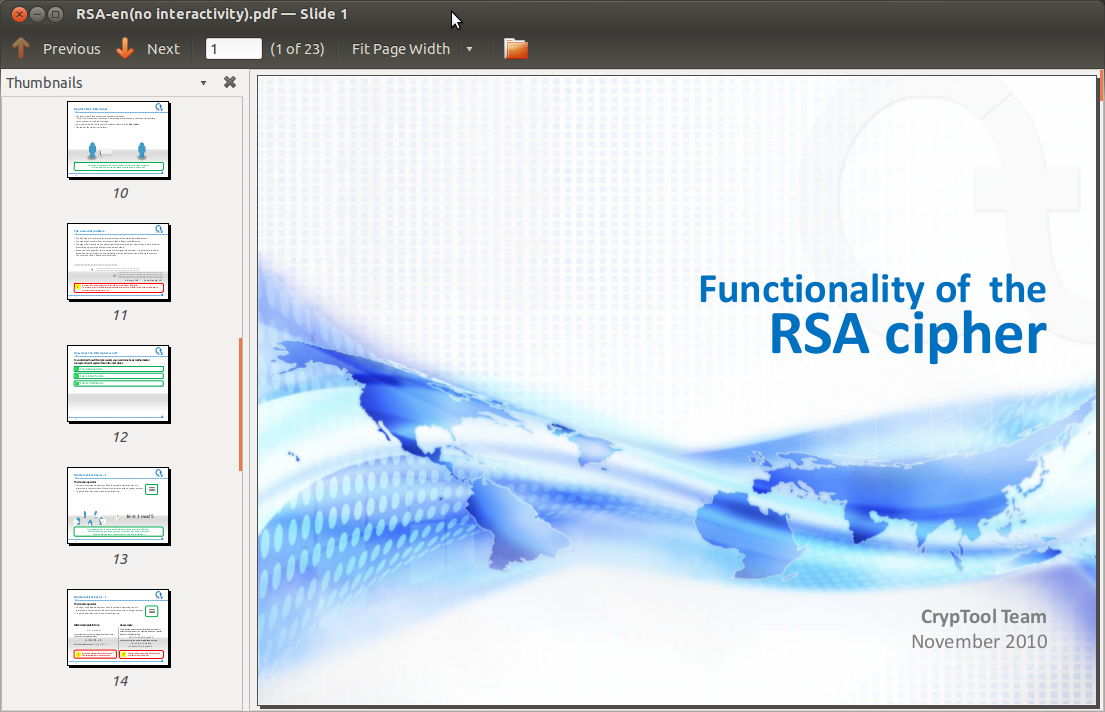
\includegraphics[scale=0.4]{figures/Interactive_RSA_Presentation_E.png}
\caption{Screenshot RSA Presentation (PDF)} 
\label{l_Interactive_RSA_Presentation}
\end{center}
\end{figure}



% ++++++++++++++++++++++++++++++++++++++++++++++++++++++++++++++++++++++++++
\newpage
\hypertarget{NumberTheory_Appendix_E}{}
\section{Appendix: Examples using Sage}
\label{NumberTheory_Appendix_E}{}
\index{Sage}
\index{Sage!Code examples}

\begin{ctsquote}
``She would never be able to tell her parents ... about any of this. She couldn't tell them about her code-breaking work. About her near death at the hands of the Daemon. About the shadowy entities pulling the strings of her government.''
\caption[Daniel Suarez]{Daniel Suarez\footnotemark}\index{Suarez, Daniel}
\end{ctsquote}
\addtocounter{footnote}{0}\footnotetext{Daniel Suarez, ``Freedom'',
  Dutton Adult, 2010, Chapter 19, ``Crossroad'', p. 229, Philips.}


\noindent Below you can find Sage source code related to contents of the
chapter~\ref{Chapter_ElementaryNT} (``\nameref{Chapter_ElementaryNT}''). 


% ---------------------------------------------------------------------------
\hypertarget{nt:AppArith1}{}
\subsection{Multiplication table modulo m}     % $ removed at $m$
\label{nt:AppArith1}{}

The multiplication table~\ref{mulmod17} (from page \pageref{SrcArith1a})
for $a \times i \pmod{m}$, where
$m = 17$, $a=5$ and $a=6$, and $i$ ranges over all integers from $0$ to $16$
can be computed using Sage as follows:

\begin{sagecode}
\begin{Verbatim}%
[fontsize=\footnotesize,fontshape=tt]
sage: m = 17; a = 5; b = 6
sage: [mod(a * i, m).lift() for i in xrange(m)]
[0, 5, 10, 15, 3, 8, 13, 1, 6, 11, 16, 4, 9, 14, 2, 7, 12]
sage: [mod(b * i, m).lift() for i in xrange(m)]
[0, 6, 12, 1, 7, 13, 2, 8, 14, 3, 9, 15, 4, 10, 16, 5, 11]
\end{Verbatim}
\caption{Multiplication tables for $a \times i \pmod{m}$ with $m = 17$, $a=5$ and $a=6$}
\end{sagecode}

\noindent The function \verb!mod()! returns an object that represents
integers modulo $m$ (in our case $m = 17$).
From the {\tt Mod} object you can get its single components either with the function
\texttt{component} or with the function \texttt{lift}.
We use the method \verb!lift()! to convert that object to an integer representation.

The other multiplication table examples modulo $13$ (table~\ref{mulmod13})
and modulo $12$ (table~\ref{mulmod12}) on page
\pageref{SrcArith1b} can similarly be computed by replacing {\tt m = 17}
with {\tt m = 13} and {\tt m = 12} respectively.


% ---------------------------------------------------------------------------
\vskip +25 pt
\hypertarget{nt:AppArith2}{}
\subsection{Fast exponentiation}
\label{nt:AppArith2}{}

The fast exponentiation modulo $m$ can be computed using the Sage
function \verb!power_mod()!. The result of this function is an
integer. We can compute the exponentiation in the example in chapter
``\nameref{hohpot}'' on page \pageref{SrcArith2} as follows:

\begin{sagecode}
\begin{Verbatim}%
[fontsize=\footnotesize,fontshape=tt]
sage: a = 87; m = 103
sage: exp = [2, 4, 8, 16, 32, 43]
sage: [power_mod(a, e, m) for e in exp]
[50, 28, 63, 55, 38, 85]
\end{Verbatim}
\caption{Fast exponentiation mod $m = 103$}
\end{sagecode}


% ---------------------------------------------------------------------------
\newpage
\hypertarget{nt:AppArith3a1}{}
\subsection{Multiplicative order}
\label{nt:AppArith3a1}{}

\noindent The order $\text{ord}_m(a)$ of a number $a$ in the multiplicative
group $\mathbf{Z}_m^{\ast}$ is the smallest number $i \geq 1$ such that
$a^i \equiv 1 \pmod{m}$ holds
(see chapter~\ref{MultOrdPrimitveRoot}, ``\nameref{MultOrdPrimitveRoot}'').
To create table~\ref{expmod11} on page~\pageref{SrcArith3a} we can print
all exponentiation $a^i \pmod{11}$ as follows:

\begin{sagecode}
\begin{Verbatim}%
[fontsize=\footnotesize,fontshape=tt]
sage: m = 11
sage: for a in xrange(1, m):
....:     print [power_mod(a, i, m) for i in xrange(1, m)]
....:
[1, 1, 1, 1, 1, 1, 1, 1, 1, 1]
[2, 4, 8, 5, 10, 9, 7, 3, 6, 1]
[3, 9, 5, 4, 1, 3, 9, 5, 4, 1]
[4, 5, 9, 3, 1, 4, 5, 9, 3, 1]
[5, 3, 4, 9, 1, 5, 3, 4, 9, 1]
[6, 3, 7, 9, 10, 5, 8, 4, 2, 1]
[7, 5, 2, 3, 10, 4, 6, 9, 8, 1]
[8, 9, 6, 4, 10, 3, 2, 5, 7, 1]
[9, 4, 3, 5, 1, 9, 4, 3, 5, 1]
[10, 1, 10, 1, 10, 1, 10, 1, 10, 1]

and including the last column with the order of each a mod (11)

sage: m = 11
sage: for a in xrange(1, m):
....:     lst= [power_mod(a, i, m) for i in xrange(1, m)]
....:     lst.append(multiplicative_order(mod(a,m)))
....:     print lst
....:
[1, 1, 1, 1, 1, 1, 1, 1, 1, 1, 1]
[2, 4, 8, 5, 10, 9, 7, 3, 6, 1, 10]
[3, 9, 5, 4, 1, 3, 9, 5, 4, 1, 5]
[4, 5, 9, 3, 1, 4, 5, 9, 3, 1, 5]
[5, 3, 4, 9, 1, 5, 3, 4, 9, 1, 5]
[6, 3, 7, 9, 10, 5, 8, 4, 2, 1, 10]
[7, 5, 2, 3, 10, 4, 6, 9, 8, 1, 10]
[8, 9, 6, 4, 10, 3, 2, 5, 7, 1, 10]
[9, 4, 3, 5, 1, 9, 4, 3, 5, 1, 5]
[10, 1, 10, 1, 10, 1, 10, 1, 10, 1, 2]
\end{Verbatim}
\caption{Table with all powers $a^i \pmod{m}$ for $m=11$, $a=1,...,10$}
\label{nt_Sage-code_MultOrder_expmod11}%Creates table with label expmod11
\end{sagecode}


\newpage
\hypertarget{nt:AppArith3b}{}
\label{nt:AppArith3b}{}

\noindent Table~\ref{expmod45} on page~\pageref{SrcArith3b} gives examples for the order modulo
45 $\text{ord}_{45}(a)$ and the Euler number $J(45)$.

\noindent The following Sage code constructs a table similar to that on page~\pageref{SrcArith3b}.

\begin{sagecode}
\begin{Verbatim}%
[fontsize=\footnotesize,fontshape=tt]
sage: m = 45
sage: for a in xrange(1, 13):
....:     lst = [power_mod(a, i, m) for i in xrange(1, 13)]
....:     try:
....:         lst.append(multiplicative_order(mod(a, m)))
....:     except:
....:         lst.append("None")
....:     lst.append(euler_phi(m))
....:     print lst
....:
[1, 1, 1, 1, 1, 1, 1, 1, 1, 1, 1, 1, 1, 24]
[2, 4, 8, 16, 32, 19, 38, 31, 17, 34, 23, 1, 12, 24]
[3, 9, 27, 36, 18, 9, 27, 36, 18, 9, 27, 36, 'None', 24]
[4, 16, 19, 31, 34, 1, 4, 16, 19, 31, 34, 1, 6, 24]
[5, 25, 35, 40, 20, 10, 5, 25, 35, 40, 20, 10, 'None', 24]
[6, 36, 36, 36, 36, 36, 36, 36, 36, 36, 36, 36, 'None', 24]
[7, 4, 28, 16, 22, 19, 43, 31, 37, 34, 13, 1, 12, 24]
[8, 19, 17, 1, 8, 19, 17, 1, 8, 19, 17, 1, 4, 24]
[9, 36, 9, 36, 9, 36, 9, 36, 9, 36, 9, 36, 'None', 24]
[10, 10, 10, 10, 10, 10, 10, 10, 10, 10, 10, 10, 'None', 24]
[11, 31, 26, 16, 41, 1, 11, 31, 26, 16, 41, 1, 6, 24]
[12, 9, 18, 36, 27, 9, 18, 36, 27, 9, 18, 36, 'None', 24]
\end{Verbatim}
\caption{Table with all powers $a^i \pmod{45}$ for $a=1,...,12$ plus the order of a}
\label{nt_Sage-code_MultOrder_expmod45}
\end{sagecode}

The number $\text{ord}_m(a)$ only exists if $a$ is relatively prime
\index{Number!co-prime} to $m$, which can be checked with \verb!gcd(a, m)!.

In the above code example, we put the calculation of the multiplicative order
within a \verb!try!-\verb!except! block. This allows Sage to catch any
exceptions or errors raised by the function \verb!multiplicative_order()!.
If an exception or error is raised in the \verb!try! block, then we know
that $\text{ord}_m(a)$ does not exist for that particular value of $a$,
hence in the \verb!except! block we append the string \verb!"None"! to
the row as represented by the object \verb!lst!.


\newpage
\hypertarget{nt:AppArith3c}{}
\label{nt:AppArith3c}{}

\noindent Table~\ref{expmod46} on page~\pageref{SrcArith3c} displays exponentiation
$a^i \pmod{46}$ as well as the order $\text{ord}_{46}(a)$.

\noindent Sage can create that table as follows:

\begin{sagecode}
\begin{Verbatim}%
[fontsize=\footnotesize,fontshape=tt]
sage: m = 46
sage: euler_phi(m)
22
sage: for a in xrange(1, 24):
....:     lst = [power_mod(a, i, m) for i in xrange(1, 24)]
....:     try:
....:         lst.append(multiplicative_order(mod(a, m)))
....:     except:
....:         lst.append("None")
....:     print lst
....:
[1, 1, 1, 1, 1, 1, 1, 1, 1, 1, 1, 1, 1, 1, 1, 1, 1, 1, 1, 1, 1, 1, 1, 1]
[2, 4, 8, 16, 32, 18, 36, 26, 6, 12, 24, 2, 4, 8, 16, 32, 18, 36, 26, 6, 12, 24, 2, 'None']
[3, 9, 27, 35, 13, 39, 25, 29, 41, 31, 1, 3, 9, 27, 35, 13, 39, 25, 29, 41, 31, 1, 3, 11]
[4, 16, 18, 26, 12, 2, 8, 32, 36, 6, 24, 4, 16, 18, 26, 12, 2, 8, 32, 36, 6, 24, 4, 'None']
[5, 25, 33, 27, 43, 31, 17, 39, 11, 9, 45, 41, 21, 13, 19, 3, 15, 29, 7, 35, 37, 1, 5, 22]
[6, 36, 32, 8, 2, 12, 26, 18, 16, 4, 24, 6, 36, 32, 8, 2, 12, 26, 18, 16, 4, 24, 6, 'None']
[7, 3, 21, 9, 17, 27, 5, 35, 15, 13, 45, 39, 43, 25, 37, 29, 19, 41, 11, 31, 33, 1, 7, 22]
[8, 18, 6, 2, 16, 36, 12, 4, 32, 26, 24, 8, 18, 6, 2, 16, 36, 12, 4, 32, 26, 24, 8, 'None']
[9, 35, 39, 29, 31, 3, 27, 13, 25, 41, 1, 9, 35, 39, 29, 31, 3, 27, 13, 25, 41, 1, 9, 11]
[10, 8, 34, 18, 42, 6, 14, 2, 20, 16, 22, 36, 38, 12, 28, 4, 40, 32, 44, 26, 30, 24, 10, 'None']
[11, 29, 43, 13, 5, 9, 7, 31, 19, 25, 45, 35, 17, 3, 33, 41, 37, 39, 15, 27, 21, 1, 11, 22]
[12, 6, 26, 36, 18, 32, 16, 8, 4, 2, 24, 12, 6, 26, 36, 18, 32, 16, 8, 4, 2, 24, 12, 'None']
[13, 31, 35, 41, 27, 29, 9, 25, 3, 39, 1, 13, 31, 35, 41, 27, 29, 9, 25, 3, 39, 1, 13, 11]
[14, 12, 30, 6, 38, 26, 42, 36, 44, 18, 22, 32, 34, 16, 40, 8, 20, 4, 10, 2, 28, 24, 14, 'None']
[15, 41, 17, 25, 7, 13, 11, 27, 37, 3, 45, 31, 5, 29, 21, 39, 33, 35, 19, 9, 43, 1, 15, 22]
[16, 26, 2, 32, 6, 4, 18, 12, 8, 36, 24, 16, 26, 2, 32, 6, 4, 18, 12, 8, 36, 24, 16, 'None']
[17, 13, 37, 31, 21, 35, 43, 41, 7, 27, 45, 29, 33, 9, 15, 25, 11, 3, 5, 39, 19, 1, 17, 22]
[18, 2, 36, 4, 26, 8, 6, 16, 12, 32, 24, 18, 2, 36, 4, 26, 8, 6, 16, 12, 32, 24, 18, 'None']
[19, 39, 5, 3, 11, 25, 15, 9, 33, 29, 45, 27, 7, 41, 43, 35, 21, 31, 37, 13, 17, 1, 19, 22]
[20, 32, 42, 12, 10, 16, 44, 6, 28, 8, 22, 26, 14, 4, 34, 36, 30, 2, 40, 18, 38, 24, 20, 'None']
[21, 27, 15, 39, 37, 41, 33, 3, 17, 35, 45, 25, 19, 31, 7, 9, 5, 13, 43, 29, 11, 1, 21, 22]
[22, 24, 22, 24, 22, 24, 22, 24, 22, 24, 22, 24, 22, 24, 22, 24, 22, 24, 22, 24, 22, 24, 22, 'None']
[23, 23, 23, 23, 23, 23, 23, 23, 23, 23, 23, 23, 23, 23, 23, 23, 23, 23, 23, 23, 23, 23, 23, 'None']
\end{Verbatim}
\caption{Table with all powers $a^i \pmod{46}$ for $a=1,...,23$ plus the order of a}
\label{nt_Sage-code_MultOrder_expmod46}
\end{sagecode}



\newpage
\hypertarget{nt:AppArith3d}{}
\label{nt:AppArith3d}{}
The following code for generating the tables~\ref{expmod14} and~\ref{expmod22}
at page~\pageref{expmod14} f. also delivers the result in a way, that in can be
easily processed in LaTeX. The prerequisite is that all content is assigned to
one Sage object (here a matrix).\footnote{%
        Remark about the Sage program, especially the Sage
        indices\index{Sage}\index{Sage!latex()}:
        \begin{compactitem}
         \item for x in xrange(2, 5) delivers 2,3,4.
         \item m = matrix(ZZ, 2, 5) has 2 rows and 5 columns.\\
               The cells are named m(0,0) to m(1,4).
         \item All elements of the matrix have to be numerical,
               so ``0'' instead of ``None'' as in the tables before.
         \item The output of matrices can be controlled in Sage with:
\begin{Verbatim}
               sage: from sage.matrix.matrix0 import set_max_cols, set_max_rows
               sage: set_max_cols(100)
               sage: set_max_rows(100)
\end{Verbatim}
         \item The length of the cycle in the last column of the tables~\ref{expmod14}
               and~\ref{expmod22} was added manually.
        \end{compactitem}
        \vspace{-\baselineskip} % Here its necessary, so that all fit to one page!
        }

\begin{sagecode}
\begin{Verbatim}%
[fontsize=\footnotesize,fontshape=tt]
def power_mod_order_matrix(m, max_a, max_i):
    r = matrix(ZZ, max_a+1, max_i+3)
    for a in xrange(0, max_a+1):
        r[a, 0] = a
        for i in xrange(1, max_i+1):
            if a==0:
                r[a,i] = i
            else:
                r[a, i] = power_mod(a, i, m)
        try:
            r[a, max_i+1] = multiplicative_order(mod(a, m))
        except:
            r[a, max_i+1] = 0
        r[a, max_i+2] = euler_phi(m)
    return r

print "\n1: m=45;max_i=13;max_a=13";m=45;max_i=13;max_a=13
r = power_mod_order_matrix(m, max_a, max_i);print r;print latex(r)

print "\n2: m=46;max_i=25;max_a=25";m=46;max_i=25;max_a=25
r = power_mod_order_matrix(m, max_a, max_i);print r.str();print latex(r)

print "\n3: m=14;max_i=13;max_a=16";m=14;max_i=13;max_a=16
r = power_mod_order_matrix(m, max_a, max_i);print r;print latex(r)

print "\n4: m=22;max_i=21;max_a=25";m=22;max_i=21;max_a=25
r = power_mod_order_matrix(m, max_a, max_i);print r.str();print latex(r)
...
3: m=14;max_i=13;max_a=16
[ 0  1  2  3  4  5  6  7  8  9 10 11 12 13  0  6]
[ 1  1  1  1  1  1  1  1  1  1  1  1  1  1  1  6]
[ 2  2  4  8  2  4  8  2  4  8  2  4  8  2  0  6]
[ 3  3  9 13 11  5  1  3  9 13 11  5  1  3  6  6]
...
\left(\begin{array}{rrrrrrrrrrrrrrrr}
0 & 1 & 2 & 3 & 4 & 5 & 6 & 7 & 8 & 9 & 10 & 11 & 12 & 13 & 0 & 6 \\
1 & 1 & 1 & 1 & 1 & 1 & 1 & 1 & 1 & 1 & 1 & 1 & 1 & 1 & 1 & 6 \\
2 & 2 & 4 & 8 & 2 & 4 & 8 & 2 & 4 & 8 & 2 & 4 & 8 & 2 & 0 & 6 \\
3 & 3 & 9 & 13 & 11 & 5 & 1 & 3 & 9 & 13 & 11 & 5 & 1 & 3 & 6 & 6 \\
...
\end{Verbatim}
\caption{Code for tables with all powers $a^i \pmod{m}$ for variable $a$ and $i$ plus order of a and Eulerphi of m}
\end{sagecode}




% ---------------------------------------------------------------------------
\newpage
\hypertarget{nt:AppArith3a2}{}
\subsection{Primitive roots}
\label{nt:AppArith3a2}
\label{primitive-roots-with-sage}
\index{Primitive root}

Computing a primitive root (see chapter~\ref{MultOrdPrimitveRoot},
``\nameref{MultOrdPrimitveRoot}'')
in Sage is very straightforward. If \verb!n! is an integer, the command
\verb!primitive_root(n)! computes \textit{one} primitive root of the multiplicative group
$(\mathbf{Z} / n \mathbf{Z})^{\ast}$, if one exists.
Where $n$ is prime, then this is the same as calculating a primitive root of
$\mathbf{Z} / n \mathbf{Z}$.

\noindent Here, we calculate some primitive roots of a few integers.

\begin{sagecode}
\begin{Verbatim}%
[fontsize=\footnotesize,fontshape=tt]
sage: primitive_root(4)
3
sage: primitive_root(22)
13
sage: for p in primes(1, 50):
....:     print p, primitive_root(p)
....:     
2 1
3 2
5 2
7 3
11 2
13 2
17 3
19 2
23 5
29 2
31 3
37 2
41 6
43 3
47 5
\end{Verbatim}
\caption{Calculating one primitive root for a given prime}
\end{sagecode}

\noindent If $p$ is prime, then $\mathbf{Z} / p \mathbf{Z}$ has at least one
primitive root.



\newpage
\noindent Sometimes we want to compute \texttt{all} the primitive roots
of $\mathbf{Z} / p \mathbf{Z}$, not just any primitive root of
$\mathbf{Z} / p \mathbf{Z}$.
The following function can do this%
\footnote{This code was developed in a Sage script file and
executed non-interactively. That is why you don't see "sage:" and "....:"
at the beginning of the lines like in the Sage samples before.}.

\begin{sagecode}
\begin{Verbatim}%
[fontsize=\footnotesize,fontshape=tt]
def enum_PrimitiveRoots_of_an_Integer(M):
    r"""
    Return all the primitive roots of the integer M (if possible).
    """
    try:
        g = primitive_root(M)
    except:
        return None
    targetOrder = euler_phi(M)
    L=[]
    # Stepping through all odd integers from 1 up to M, not including
    # M. So this loop only considers values of i where 1 <= i < M.
    for i in xrange(1,M,2):
            testGen = Mod(g^i,M)
            if testGen.multiplicative_order() == targetOrder:
                L.append(testGen.lift())
    # removing duplicates
    return Set(L)

# AA_Start -- Testcases for enum_PrimitiveRoots_of_an_Integer(M)
print "AA_Start -- Testcases for enum_PrimitiveRoots_of_an_Integer(M)"
M=10; print "1-----------Testcase: M = %s" % M
LL = enum_PrimitiveRoots_of_an_Integer(M)
if LL==None:
    print M
else:
    print LL
M=8; print "2-----------Testcase: M = %s" % M
# M=8 hat keine primitive root mod m. Checke, ob per try - except abgefangen.
LL = enum_PrimitiveRoots_of_an_Integer(M)
if LL==None:
    print M
else:
    print LL
M=17; print "3-----------Testcase: M = %s" % M
LL = enum_PrimitiveRoots_of_an_Integer(M)
if LL==None:
    print M
else:
    print LL
# AA_End -- Testcases

OUTPUT:
AA_Start -- Testcases for enum_PrimitiveRoots_of_an_Integer(M)
1-----------Testcase: M = 10
{3, 7}
2-----------Testcase: M = 8
8
3-----------Testcase: M = 17
{3, 5, 6, 7, 10, 11, 12, 14}
\end{Verbatim}
\caption{Function ``enum\_PrimitiveRoots\_of\_an\_Integer'' to calculate all primitive
roots for a given number}
\end{sagecode}



\newpage
\noindent For example, here is a list of all primitive roots of the prime 541.

\begin{sagecode}
\begin{Verbatim}%
[fontsize=\footnotesize,fontshape=tt]
sage: L=enum_PrimitiveRoots_of_an_Integer(541); L
{2, 517, 10, 523, 13, 14, 527, 528, 18, 531, 24, 539, 30, 37, 40, 51,
54, 55, 59, 62, 65, 67, 68, 72, 73, 77, 83, 86, 87, 91, 94, 96, 98,
99, 107, 113, 114, 116, 117, 126, 127, 128, 131, 132, 138, 150, 152,
153, 156, 158, 163, 176, 181, 183, 184, 195, 197, 199, 206, 208,
210, 213, 218, 220, 223, 224, 244, 248, 250, 257, 258, 259, 260,
261, 263, 267, 269, 270, 271, 272, 274, 278, 280, 281, 282, 283,
284, 291, 293, 297, 317, 318, 321, 323, 328, 331, 333, 335, 342,
344, 346, 357, 358, 360, 365, 378, 383, 385, 388, 389, 391, 403,
409, 410, 413, 414, 415, 424, 425, 427, 428, 434, 442, 443, 445,
447, 450, 454, 455, 458, 464, 468, 469, 473, 474, 476, 479, 482,
486, 487, 490, 501, 504, 511}
sage: len(L)
144
\end{Verbatim}
\caption{Table with all primitive roots for the given prime 541}
\end{sagecode}



\newpage
\noindent With a little bit of programming, we can count how many primitive roots
are in a given range of integers. We can check this for all numbers or only for the
primes within this range.

\begin{sagecode}
\begin{Verbatim}%
[fontsize=\footnotesize,fontshape=tt]
def count_PrimitiveRoots_of_an_IntegerRange(start, end, bPrimesOnly=True):
	r"""
	Compute all primitive roots of all numbers between start and end,
	inclusive, and count them.
	If the flag bPrimesOnly is True, it performs primality tests, so it
	allows us to count the number of primes from start to end, inclusive.
        If the flag bPrimesOnly is false, it additionally counts these even
	numbers which have no primitive root.
	"""
	nCheckedNumb = 0
	nCheckedNumb_WithoutPrimitivRoots = 0
	nPrimitiveRoots = 0
	for n in xrange(start, end+1):
		if bPrimesOnly:
			if is_prime(n):
				nCheckedNumb += 1
				L = enum_PrimitiveRoots_of_an_Integer(n)
				nPrimitiveRoots += len(L)
		else:
			nCheckedNumb += 1
			L = enum_PrimitiveRoots_of_an_Integer(n)
			if L==None:
				nCheckedNumb_WithoutPrimitivRoots += 1
			else:
				nPrimitiveRoots += len(L)

	if bPrimesOnly:
		print "Found all %s" % nPrimitiveRoots + \
		      " primitive roots of %s primes." % nCheckedNumb
	else:
		if nCheckedNumb_WithoutPrimitivRoots == 0:
			print "Found all %s " % nPrimitiveRoots + \
			      "primitive roots of %s numbers." % nCheckedNumb
		else:
			print "Found all %s " % nPrimitiveRoots + \
			      "primitive roots of %s numbers." % \
			          (nCheckedNumb - nCheckedNumb_WithoutPrimitivRoots)
			print "(Total of numbers checked: %s, " % nCheckedNumb + \
			      "Amount of numbers without primitive roots: %s)" % \
			          nCheckedNumb_WithoutPrimitivRoots
\end{Verbatim}
\caption{Function ``count\_PrimitiveRoots\_of\_an\_IntegerRange'' to calculate all
primitive roots for a given range of integers}
\end{sagecode}


\newpage
\noindent Using the Sage command \verb!time!, we can also find out how long it takes on
our computer.

\begin{sagecode}
\begin{Verbatim}%
[fontsize=\footnotesize,fontshape=tt]
# BB_Start -- Testcases for count_PrimitiveRoots_of_an_IntegerRange(start, end, bPrimesOnly=True)
print "\n\nBB_Start -- Testcases for count_PrimitiveRoots_of_an_IntegerRange(start, end, True)"

print "\n1-----------Testcase: (1, 500)"
time count_PrimitiveRoots_of_an_IntegerRange(1, 500)

print "\n2-----------Testcase: (5, 6, False)"
time count_PrimitiveRoots_of_an_IntegerRange(5, 6, False)

print "\n3-----------Testcase: (1, 500, False)"
time count_PrimitiveRoots_of_an_IntegerRange(1, 500, False)
# BB_End -- Testcases

OUTPUT:
BB_Start -- Testcases for count_PrimitiveRoots_of_an_IntegerRange(start, end, bPrimesOnly=True)

1-----------Testcase: (1, 500)
Found all 8070 primitive roots of 95 primes.
Time: CPU 0.94 s, Wall: 0.97 s

2-----------Testcase: (5, 6, False)
Found all 3 primitive roots of 2 numbers.
Time: CPU 0.00 s, Wall: 0.00 s

3-----------Testcase: (1, 500, False)
Found all 11010 primitive roots of 170 numbers.
(Total of numbers checked: 500, Amount of numbers without primitive roots: 330)
Time: CPU 1.52 s, Wall: 1.59 s
\end{Verbatim}
\caption{Function ``count\_PrimitiveRoots\_of\_an\_IntegerRange'': testcases and output}
\end{sagecode}




\newpage
\noindent Using our custom-defined function \verb!enum_PrimitiveRoots_of_an_Integer!,
we can find all primitive roots of one prime integer $p$.

The following function counts how many primes are in a given range
and enumerate all their primitive roots.

From this list of primitive roots, we can determine the smallest and largest
primitive root for $\mathbf{Z} / p \mathbf{Z}$, as well as count the number
of primitive roots of $\mathbf{Z} / p \mathbf{Z}$.

\begin{sagecode}
\begin{Verbatim}%
[fontsize=\footnotesize,fontshape=tt]
def count_PrimitiveRoots_of_a_PrimesRange(start, end):
      r"""
      Compute all primitive roots of all primes between start and end,
      inclusive. This uses a primes iterator.
      """
      nPrimes = 0
      nPrimitiveRoots = 0
      for p in primes(start, end+1):
          L = enum_PrimitiveRoots_of_an_Integer(p)
	  print p, len(L)
          nPrimes += 1
          nPrimitiveRoots += len(L)
      print "Found all %s" % nPrimitiveRoots + " primitive roots of %s primes." % nPrimes

# CC_Start -- Testcases for count_PrimitiveRoots_of_a_PrimesRange(start, end)
print "\n\nBB_Start -- Testcases for count_PrimitiveRoots_of_a_PrimesRange(start, end)"
print "-----------Testcase: (1, 1500)"
time count_PrimitiveRoots_of_a_PrimesRange(1, 1500)
# CC_End -- Testcases

OUTPUT:
CC_Start -- Testcases for count_PrimitiveRoots_of_a_PrimesRange(start, end)
-----------Testcase: (1, 1500)
2 1
3 1
5 2
7 2
11 4
13 4
17 8
19 6
23 10
29 12
31 8
37 12
...
1483 432
1487 742
1489 480
1493 744
1499 636
Found all 62044 primitive roots of 239 primes.
Time: CPU 7.55 s, Wall: 7.85 s
\end{Verbatim}
\caption{Function ``count\_PrimitiveRoots\_of\_a\_PrimesRange'' to calculate the number
of primitive roots for a given range of primes}
\end{sagecode}



\newpage
\noindent A slightly modified version of our function
\verb!count_PrimitiveRoots_of_a_PrimesRange!, was used to generate
a database of all primitive roots of all primes between 1 and 100,000.

\begin{sagecode}
\begin{Verbatim}%
[fontsize=\footnotesize,fontshape=tt]
start = 1
end = 10^5
fileName = "/scratch/mvngu/primroots.dat"
file = open(fileName, "w")
for p in primes(start, end+1):
    L = enum_PrimitiveRoots_of_an_Integer(p)
    print p, len(L)
    # Output to a file. The format is:
    # (1) the prime number p under consideration
    # (2) the number of primitive roots of Z/pZ
    # (3) all the primitive roots of Z/pZ
    file.write(str(p) + " " + str(len(L)) + " " + str(L) + "\n")
    file.flush()
file.close()
\end{Verbatim}
\caption{Code to generate the database with all primitive roots for all primes between
1 and 100,000}
\end{sagecode}

It took about one day on the machine sage.math to generate the
file ``primroots.dat'' (done in July 2009 by Minh Van Nguyen).

This code and the function \verb!enum_PrimitiveRoots_of_an_Integer!
was put in a Sage script file and executed non-interactively.

The file ``primroots.dat'' is a database of all primitive roots of all primes
between 1 and 100,000 inclusive. It is a very large file (about 1 GB
uncompressed, and 285 MB compressed with bzip2). You can find the file
at {\url{http://sage.math.washington.edu/home/mvngu/doc/primitive-roots/primroots.dat.bz2}}.



\newpage
\noindent This database file ``primroots.dat'' was used then to create three graphics using the following code.

\begin{sagecode}
\begin{Verbatim}%
[fontsize=\footnotesize,fontshape=tt]
sage: # open a database file on primitive roots from 1 to 100,000
sage: file = open("/scratch/mvngu/primroots.dat", "r")
sage: plist = []    # list of all primes from 1 to 100,000
sage: nlist = []    # number of primitive roots modulo prime p
sage: minlist = []  # smallest primitive root modulo prime p
sage: maxlist = []  # largest primitive root modulo prime p
sage: for line in file:
....:     # get a line from the database file and tokenize it for processing
....:     line = line.strip().split(" ", 2)
....:     # extract the prime number p in question
....:     plist.append(Integer(line[0]))
....:     # extract the number of primitive roots modulo p
....:     nlist.append(Integer(line[1]))
....:     # extract the list of all primitive roots modulo p
....:     line = line[-1]
....:     line = line.replace("{", "")
....:     line = line.replace("}", "")
....:     line = line.split(", ")
....:     # sort the list in non-decreasing order
....:     line = [Integer(s) for s in line]
....:     line.sort()
....:     # get the smallest primitive root modulo p
....:     minlist.append(line[0])
....:     # get the largest primitive root modulo p
....:     maxlist.append(line[-1])
....:
sage: file.close()  # close the database file
sage: # plot of number of primitive roots modulo p
sage: nplot = point2d(zip(plist, nlist), pointsize=1)
sage: nplot.axes_labels(["x", "y"])
sage: nplot
sage: # plot of smallest primitive root modulo prime p
sage: minplot = point2d(zip(plist, minlist), pointsize=1)
sage: minplot.axes_labels(["x", "y"])
sage: minplot
sage: # plot of largest primitive root modulo prime p
sage: maxplot = point2d(zip(plist, maxlist), pointsize=1)
sage: maxplot.axes_labels(["x", "y"])
sage: maxplot
\end{Verbatim}
\caption{Code to generate the graphics about the primitive roots}
\end{sagecode}




\newpage
Figure~\ref{fig:primitive_roots_all} graphs the number of primitive
roots for each prime between 1 and 100,000. The $x$-axis represents
primes between 1 and 100,000, while the $y$-axis counts the number of
primitive roots for each prime within that interval.

\begin{figure}[!htbp]
\centering
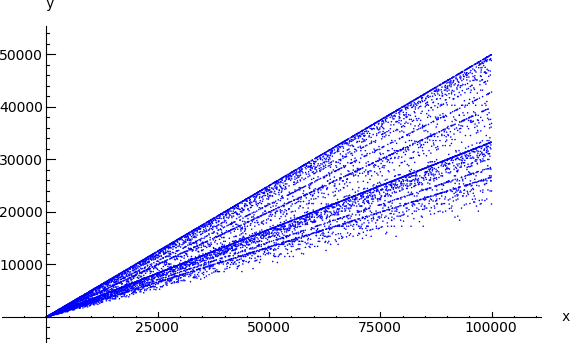
\includegraphics{figures/primitive-roots-all}
\caption{The number of primitive roots of all primes between 1 and 100,000.}
\label{fig:primitive_roots_all}
\end{figure}

\vskip +50 pt
Figure~\ref{fig:primitive_roots_smallest} graphs the smallest
primitive roots of all primes between 1 and 100,000. The $x$-axis
represents primes between 1 and 100,000. The $y$-axis represents the
smallest primitive root of each prime within that
interval.

\vskip +25 pt
Figure~\ref{fig:primitive_roots_largest} shows a
corresponding graph for the largest primitive root of each prime
within the above interval.

\begin{figure}[!htbp]
\centering
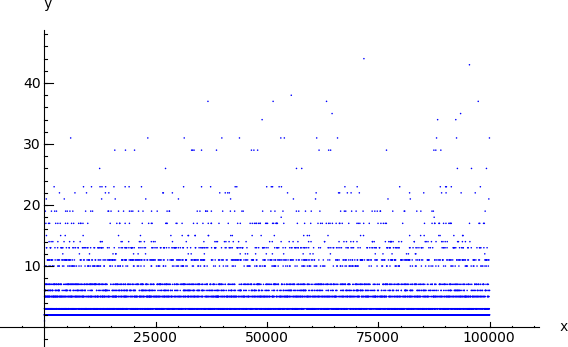
\includegraphics{figures/primitive-roots-smallest}
\caption{The smallest primitive roots of all primes between 1 and 100,000.}
\label{fig:primitive_roots_smallest}
\end{figure}

\begin{figure}[!htbp]
\centering
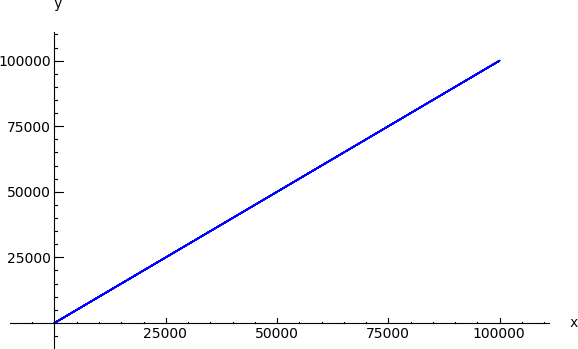
\includegraphics{figures/primitive-roots-largest}
\caption{The largest primitive roots of all primes between 1 and 100,000.}
\label{fig:primitive_roots_largest}
\end{figure}




% ---------------------------------------------------------------------------
\newpage
\hypertarget{NumberTheory_Sage_RSA sample}{}
\subsection{RSA examples with Sage}
\label{l:NumberTheory_Sage_RSA sample}{}

\noindent Below is Sage source code for the simple RSA examples in
section~\ref{rsaconcrete} (``\nameref{rsaconcrete}''). 

\vskip +10 pt 
\hypertarget{nt:AppArith4a}{%
\noindent \textbf{Example on page~\pageref{SrcArith4a}:}}
\label{nt:AppArith4a}\\
The RSA exponentiation $M^{37} \pmod{3713}$ on message $M = 120$ can be
calculated in Sage as follows:

\begin{Verbatim}%
[fontsize=\footnotesize,fontshape=tt]
sage: power_mod(120, 37, 3713)
1404
\end{Verbatim}


\vskip +10 pt 
\hypertarget{nt:AppArith4b}{%
\noindent {\bf Example on page~\pageref{SrcArith4b}:}}
\label{nt:AppArith4b}\\
The factorization of $J(256027) = 255016 = 2^3 * 127 * 251$ can be
calculated using Sage as follows:

\begin{sagecode}
\begin{Verbatim}%
[fontsize=\footnotesize,fontshape=tt]
sage: factor(255016)
2^3 * 127 * 251
\end{Verbatim}
\caption{Factoring a number}
\end{sagecode}


\vskip +10 pt 
\hypertarget{nt:AppArith4c}{%
\noindent {\bf Example on page~\pageref{SrcArith4c}:}}
\label{nt:AppArith4c}\\
Sage can do RSA encryption as follows:

\begin{sagecode}
\begin{Verbatim}%
[fontsize=\footnotesize,fontshape=tt]
sage: A = [82, 83, 65, 32, 119, 111, 114, 107, 115, 33]
sage: e = 65537; m = 256027
sage: [power_mod(a, e, m) for a in A]
[212984, 25546, 104529, 31692, 248407, 100412, 54196, 100184, 58179, 227433]
\end{Verbatim}
\caption{RSA encryption by modular exponentiation of a number (used as message)}
\end{sagecode}


\vskip +10 pt 
\hypertarget{nt:AppArith4d}{%
\noindent {\bf Example on page~\pageref{SrcArith4d}:}}
\label{nt:AppArith4d}\\
RSA encryption using Sage:

\begin{Verbatim}%
[fontsize=\footnotesize,fontshape=tt]
sage: A = [21075, 16672, 30575, 29291, 29473]
sage: e = 65537; m = 256027
sage: [power_mod(a, e, m) for a in A]
[158721, 137346, 37358, 240130, 112898]
\end{Verbatim}


\vskip +10 pt 
\hypertarget{nt:AppArith4e}{%
\noindent {\bf Example on page~\pageref{SrcArith4e}:}}
\label{nt:AppArith4e}\\
RSA encryption using Sage:

\begin{Verbatim}%
[fontsize=\footnotesize,fontshape=tt]
sage: A = [82083, 65032, 119111, 114107, 115033]
sage: e = 65537; m = 256027
sage: [power_mod(a, e, m) for a in A]
[198967, 51405, 254571, 115318, 14251]
\end{Verbatim}




% ---------------------------------------------------------------------------
\newpage
\hypertarget{NumberTheory_Sage_Number-of-RSA-keys}{}
\subsection{How many private RSA keys $d$ exist within a given modulo range?}
\label{l:NumberTheory_Sage_Number-of-RSA-keys}{}

The RSA encryption procedure was described in section \ref{RSA} (``\nameref{RSA}'').
Steps 1 to 3 constitute key generation, steps 4 and 5 are the encryption:
\begin{itemize}
  \item[{\bf 1.}] Select two distinct random prime numbers $p$ and $q$
                  and calculate $n = p*q$.\\
                  The value $n$ is called the RSA modulus.

  \item[{\bf 2.}] Select an arbitrary $e \in \{2, \cdots, n-1\}$ such that: \\
                  $e$ is relatively prime
                  \index{Prime number!relative prime}\index{Number!relative prime}
                  to $J(n) = (p-1)*(q-1)$. \\
                  We can then ``throw away'' $p$ and $q$.

  \item[{\bf 3.}] Select $d \in \{1, \cdots, n-1\}$ with $e*d \equiv 1  
                  {\rm ~(mod~} J(n))$,\\
		  i.e. $d$ is the multiplicative inverse of $e$ modulo $J(n)$.
		  We can then ``throw away'' $J(n)$.
    \begin{compactitem}
        \item[] $\rightarrow (n, e)$ is the public key $P$.
        \item[] $\rightarrow (n, d)$ is the private key $S$ (only $d$ must be kept secret).
    \end{compactitem}

  \item[{\bf 4.}] For encryption, the message represented as a (binary) number
                  is divided into parts such that each part of 
                  the number represents a number less than $n$.

  \item[{\bf 5.}] Encryption of the plaintext (or the parts of it) $M \in \{1, \cdots, n-1\}$:
                  $$C = E ( (n, e); M ) := M^e {\rm ~(mod~} n).$$
\end{itemize}

The default way to crack a given RSA ciphertext $C$ would be to use the public key
of the recipient and to try to factorize $n$. Then you can go through the steps 2 and 3
and generate the private key $e$, which is normally used to decrypt a ciphertext.

According to the ``prime number theorem''\footnote{%
See section \ref{thm-pz-pi-x} (``\nameref{l_Primes_Distrib-of-Primes}'').
}
the number of prime numbers $PI(x)$ is asymptotic to  $x / ln(x)$.
%% So in a given range $[x,y]$ there are about $ (y / ln(y)) - (x / ln(x))$ primes.
Between $1$ and a given $n$ there are about $n / ln(n)$ different primes.
%% (not considering the more specific requirements for selecting
%%  appropriate values for $p$ as described above).

\noindent If you don't want to use factorization but ask the question like in classic
encryption, you may want to find out:
How many possible private keys $(n, d)$ are there for a given key size range
$n \in [a, b]$?\footnote{%
Chapter~\ref{L_nt_Num-of-d-mod-26} (``\nameref{L_nt_Num-of-d-mod-26}''),
p.~\pageref{L_nt_Num-of-d-mod-26} deals with the special case $n=26$.}
%% (this means, only a part of each public key $(n, e)$ is known).

\noindent Sage source code~\ref{nt_sagesample_Count_RSA_Keys} below defining the
function \verb#count_Number_of_RSA_Keys# can answer this question concretely
(if the modulus is not too big).\footnote{%
%\begin{compactitem}
\newlength{\saveleftmargini}
\setlength{\saveleftmargini}{\leftmargini}
\setlength{\leftmargini}{0em}% for example to outdent verse
\settowidth{\versewidth}{xxxxx xxxxx xxxxx xxxxx xxxxx xxxxx xxxxx xxxxx xxxxx xxxxx xxxxx xxxxx xxxxx xxxxx xxxxx xxxxx xxxxx xxxxx}
\vspace{-\baselineskip} % TODO: Geht das nicht anders?
\begin{verse}[\versewidth]
 a) Calling \verb#sage: count_Number_of_RSA_Keys(100, 1000)# means to consider the interval
$[100, 1000]$ for $n$.
\verselinebreak $n$ is defined by the two primes $p, q: n = p*q$.
\verselinebreak So here one prime can have the maximal value $500$ because $2 * 500 =1000$
(while then the other prime will have the smallest possible prime value $2$).\\
\vin The number of possible combinations of primes is $comb = 258$.\\
\vin The number of primes in the given range is $143$.\\
\vin The number of private keys is $34,816$.
\end{verse}
%\noindent %       \item
\begin{verse}[\versewidth]
 b) Calling \verb#sage: count_Number_of_RSA_Keys(100, 100, True)# has the
following output:\\
\vin    - Number of private keys for modulus in a given range: 0\\
\vin    - Number of primes in a given range: 0\\
\vin    The reason for that is, that with this call only $n=100$ is considered,
   and the function investigates only\\
\vin semiprime $n$: $100$ is not semi prime\index{Prime number!semi
   prime}\index{Prime number!half prime},
   this means $100$ is not the product of only two primes.
\end{verse}
\setlength{\leftmargini}{\saveleftmargini}% restore original value%\end{compactitem}
}


\begin{sagecode}
\begin{Verbatim}%
[fontsize=\footnotesize,fontshape=tt]
def count_Number_of_RSA_Keys(start, end, Verbose=False):
      r"""
      How many private RSA keys (n,d) exist, if only modulus N is given, and start <= N <= end?
        (prime_range(u,o) delivers all primes >=u und < o).
      """
      a = start
      b = end
      s = 0
      comb = 0
      for p in prime_range(1, b/2+1):
          for q in prime_range(p + 1, b/2+1):
              if a <= p * q and p * q <= b:
                  comb = comb +1
                  s = s + (euler_phi(euler_phi(p * q))-1)
                  if Verbose:
                      print "p=%s, " % p + "q=%s, " % q + "s=%s" % s
      print "Number of private keys d for modulus in a given range: %s" % s + " (comb=%s), " % comb

      # Just for comparison: How many primes are in this range?
      s = 0
      for p in prime_range(a, b+1):
          if Verbose:
              print "a=%s, " % a + "b=%s, " % b + "p=%s" % p
          s = s + 1
      print "Number of primes in a given range: %s" % s

print "\n\nDD_Start -- Testcases for count_Number_of_RSA_Keys(start, end)"
print "\n-----------Testcase: (100, 1000) [Should deliver 34.816]"
time count_Number_of_RSA_Keys(100, 1000)
print "\n-----------Testcase: (100, 107, True) [Should deliver 23]"
time count_Number_of_RSA_Keys(100, 107, True)
u = 10^3; o = 10^4;
print "\n-----------Testcase: (%s, " % u + "%s) [Should deliver 3.260.044]" % o
time count_Number_of_RSA_Keys(u, o)

OUTPUT:
DD_Start -- Testcases for count_Number_of_RSA_Keys(start, end)

-----------Testcase: (100, 1000) [Should deliver 34.816]
Number of private keys d for modulus in a given range: 34816 (comb=258),
Number of primes in a given range: 143
Time: CPU 0.03 s, Wall: 0.04 s

-----------Testcase: (100, 107, True) [Should deliver 23]
p=2, q=53, s=23
Number of private keys d for modulus in a given range: 23 (comb=1),
a=100, b=107, p=101
a=100, b=107, p=103
a=100, b=107, p=107
Number of primes in a given range: 3
Time: CPU 0.00 s, Wall: 0.00 s

-----------Testcase: (1000, 10000) [Should deliver 3,260,044]
Number of private keys d for modulus in a given range: 3260044 (comb=2312),
Number of primes in a given range: 1061
Time: CPU 0.63 s, Wall: 0.66 s
\end{Verbatim}
\caption{How many private RSA keys d are there if you know a range for the public key n?}
\label{nt_sagesample_Count_RSA_Keys}
\end{sagecode}

\noindent As there are many more private keys $(n, d)$ within a
bigger range of values for $n$, even brute-force factoring
is much more efficient as brute-force trying all the keys.




% ---------------------------------------------------------------------------
\clearpage
\newpage
\hypertarget{NumberTheory_Sage_Number-of-RSA-FixedPoints}{}
\subsection
    [RSA fixed points \texorpdfstring{}{m = m\^{}e}]
    {RSA fixed points $ m^e = m \bmod n $ mit $m \in \{1,...,n-1\}$ }
\label{l:NumberTheory_Sage_Number-of-RSA-FixedPoints}{}
\index{Fixpoint}\index{RSA!fixpoint}
%%% xxx111222xxx-beg

Also encryption methods can have fixed -- cleartext messages where the
according ciphertext matches the original. In mathematics, variables
mapped by the algorithm (function) onto themselves are called fixed points.
In cryptography the according messages are called ``unconcealed messages''.

Generally speaking: The more fixed points an encryption algorithm contains,
the easier it is to break it.

With the RSA procedure: $n=pq$ is the product of two different prime numbers,
and there exists $e$ where $gcd(e,(p-1)(q-1))=1$. The encription is then
$c = m^e \mod n$. 
A fixed point in the RSA procedure is a message $m$, where: 
$m = m^e \mod n$. 
The result of the encryption is the given message.

When the size of $n$ is sufficiently big, the probability of the occurance of
fixed points in RSA is very small -- as illustrated in Figure
\ref{fig:NumberFixpointsGrowingN}: In average, we found not more than 40 fixed
points.

Students often presume the occurence of fixed points high, because they counter
a ``relatively'' large number of examples when experimenting with \textbf{small}
prime numbers, as m = 0, 1 and n-1 are also always fixed points.

In practice, where large prime numbers are chosen, fixed points have no
significance for the security of RSA. Therefore, this paragraph refers more
to the mathematical questions.\footnote{%
Thanks to Taras Shevchenko for gathering parts of the content of this chapter
and to Volker Simon for writing the Sage program
\ref{nt_sagesample_Calculate_RSA-Fixpoints} ``Getfixpoints''.}


% ----------------------------------------------------
\subsubsection{The number of RSA fixed points}

In this section we show how many RSA fixed points there are for $m \in \{1,...,n-1\} $.\\

\begin{theorem}\label{nt-number-of-fixpoints-1-to-n-1}
The number of the fixed points $ m^e = m \bmod n$ with $m \in \{1,...,n-1\} $ is \\$ gcd(p-1, e-1) \cdot gcd(q-1, e-1) $.
\end{theorem}
\begin{proof}
Given $m^e = m \bmod n.$
According to the CRT\index{CRT}\footnote{%
CRT = Chinese Remainder Theorem.
\url{http://en.wikipedia.org/wiki/Chinese_Remainder_Theorem}
}, the following statements are equivalent:\\
$$ [ m^e = m \bmod n ]  \Leftrightarrow [ m^{e} = m \bmod p \text{  and  } m^{e} = m \bmod q ] $$
% STH: consider using 'analysis' instead of 'decomposition'
%      be: Kl�ren, denn es ist auch keine �quivalenz! xxxxxxxxxxxxxxxxxxxxxxxxxxxxxxxxx
This decomposition is equivalent to:
$$m^{e-1} = 1 \bmod p \text{  and  } m^{e-1} = 1 \bmod q. $$

\noindent We consider  $m^{e-1} = 1 \bmod p$ and search all $(e-1)$
roots of unity\index{RootOfUnity}\footnote{%
- In mathematics, a \textbf{root of unity} is a number $x$ that equals 1 when raised to some integer power $n$.

\noindent- An $n$-th root of unity $x$ is \textbf{primitive} if it is not a $k$-th root of unity for all integers $k$ smaller than $n$:
 $$x^{n} = 1  \text{ and }    x^{k} \neq 1 ~~~(k = 1,2, 3, ..., n-1)$$

\noindent-
If $F$ is a finite field and $n$ is a positive integer, then a $n$th-root of unity in $F$ is a solution of the equation $$ x^{n}-1 = 0 \text{ in } F $$
}
in $\mathbb{Z}_p^{*}.$\\
It holds: $\mathbb{Z}_p^{*}$ for p prime is cyclic.~~$\Rightarrow $~~
A generator $g$ exists which produces $\mathbb{Z}_p^{*}$: $\mathbb{Z}_p^{*}=<g>$.\\

\noindent The following theorem from \cite[Pg. 69]{nt:Katzenbeisser2001}\index{Katzenbeisser 2001} characterizes all $(e-1)$-th roots of unity in $\mathbb{Z}_p^{*}$:
\begin{theorem}\label{nt-katzenbeisser-Anzahl-Einheitswurzeln}
$g^{\alpha}$ is exactly then $(e-1)$-th root of unity in $\mathbb{Z}_p^{*}$,
when $(e-1)\alpha = 0\bmod p-1.$ There are $gcd(p-1, e-1)$ of these.
\end{theorem}
\begin{proof} 
The first thesis results directly from the small theorem from Fermat:
\[g^{\alpha (e-1)}= 1 \bmod p  ~~\Rightarrow~~ \alpha (e-1) = 0\bmod p-1 \]
Let $\delta =gcd(p-1, e-1)$.  $\alpha (e-1) = 0\bmod p-1$ implies $\frac{\alpha (e-1)}{\delta}= 0 \bmod \frac{p-1}{\delta}$. \\
Since $\frac {e-1}{\delta}$ and $\frac{p-1}{\delta}$ are coprime (each was 
reduced by the gcd of their corresponding numerator),
$\alpha$ must be a multiple of $\frac{p-1}{\delta}$.

\[ \alpha \frac{p-1}{\delta} ~~ \text{with} ~~ \alpha = 1,...,\delta
\]\\
These $\delta$ different powers then correspond to the 
$(e-1)$-th roots of unity $g^{\alpha \frac{p-1}{\delta}} \bmod p$ in $\mathbb{Z}_p^{*}$.
\end{proof}

\noindent Analog for $q$: For $m^{e-1} = 1 \bmod q $ we then have $ gcd(q-1, e-1) $ many of $(e-1)$-th roots of unity.\\

\noindent The number of combinations of the $(e-1)$-th root of unity in $\mathbb{Z}_p^{*}$ and
$\mathbb{Z}_q^{*}$ gives the total quantity of RSA fixed points:
$ m^e = m \bmod n$ with $ m \in \{1,...,n-1\}$:\\
 $gcd(p-1, e-1) \cdot gcd(q-1, e-1) $\\

\noindent Adding $m=0$ to the above, results in the theorem \ref{nt-thm-Anzahl-RSA-Fixpunkte}:
\begin{theorem}\label{nt-thm-Anzahl-RSA-Fixpunkte}
If $ m \in \{0,...,n-1\}$, then the quantity of the RSA fixed points is:
          \[ (gcd(p-1, e-1)+1) \cdot (gcd(q-1, e-1)+1) \]
\end{theorem}
\end{proof}
\vspace{15pt}



% ----------------------------------------------------
\subsubsection{Lower bound for the quantity of RSA fixed points}
In the following section, we show that there is a lower bound for the quantity of RSA fixed points. This lower bound $6$ exists when the two different RSA prime numbers are the smallest possible values (2 and 3).\\

\noindent\textbf{Thesis 1: $p = 2, q = 3$}\\
The quantity of RSA fixed points for $p=2$ and $q=3$ is\\
$(\underbrace{gcd(p-1, e-1)}_{=1}+1) \cdot (\underbrace{gcd(q-1, e-1)}_{=2}+1)=2 \cdot 3=6$ \\

\noindent\textbf{Thesis 2: $p \neq q; p > 2, q > 2$}\\
The quantity of RSA fixed points for $p \neq q; p,q > 2$ is $\geq 9$.

\begin{proof}
Since $p$ and $q$ are prime, $(p-1)$ and $(q-1)$ for $ p,q > 2 $ are even.\\
The RSA algorithm requires to choose e so that $1 < e < \phi(n)=(p-1)(q-1)$ and \\
$gcd(e,(p-1)(q-1))=1$\\
Since $(p-1)$ and $(q-1)$ are even, e is odd $ \Rightarrow e-1$ is even.\\
Since $(p-1)$ and $(e-1)$ are even, then:\\
$gcd(p-1, e-1) \geq 2$ \\
$\Rightarrow (gcd(p-1, e-1)+1) \geq 3$ and $(gcd(q-1, e-1)+1) \geq 3$\\
$\Rightarrow (gcd(p-1, e-1)+1) \cdot (gcd(q-1, e-1)+1) \geq 9$
\end{proof}

\noindent Samples:\\
For $(e,n)=(17,6)$, all six possible messages \{0,1,2,3,4,5\} are
fixed points (for $n=6$, it is independent from the value of $e$).\\
For $(e,n)=(17,10)$, all 10 possible messages are fixed points.\\
For $(e,n)=(19,10)$, only 6 of the 10 possible messages are fixed points.


% ----------------------------------------------------
\vspace{15pt}
%\subsubsection{Unfortunate choice of $e$ }
\subsubsection{Unfortunate choice of \texorpdfstring{$e$}{e} }
In this section, we show that with $e=1+lcm(p-1,q-1)$ each encryption results in a fixed
point (independently of the size of p,q, or n); and then we broaden this to all unfortunate
choices of $e$.\\

\noindent If $e=1$, then for all $ m$: $ c = m^e = m$. This is the trivial case.\\

\noindent\textbf{Thesis 1: $p,q > 2$}\\
If $e=1+lcm(p-1,q-1)$, then for all $ m \in \{1,...,n-1\}$: $ m^e = m \bmod n$.

\begin{proof}~\\
Given:\\
-~~~ $ ~~~ e\cdot d=1 \mod \phi(n)$ ~or~ $e\cdot d=1 \mod lcm(p-1,q-1) $\\
-~~~ $ ~~~ m^{x} \mod n = m^{x \mod \phi(n)} \mod n $\\

\noindent Encryption of messages: \\
 $~~~c=m^e \mod n$, where c is the ciphertext and m is the plaintext.

\noindent Decryption of messages:\\
 $~~~m'=c^d \mod n$, where d is the multiplicative inverse of e.\\

\noindent We will show: $c=m \mod n$ for the chosen e.

$~~~c = m^e \mod n$

$~~~c = m^{1+lcm(p-1,q-1)} \mod n$

$~~~c = m^1 \cdot m^{k \cdot (p-1) \cdot (q-1)} \mod n$

$~~~c = m^1 \cdot m^{[k \cdot \phi(n)] \mod \phi(n)} \mod n$

$~~~c = m^1 \cdot m^{0} = m \mod n $
\end{proof}

\newpage
% ~\\
\noindent\textbf{Example: Fixed point property for all m:}\\
Given $n=p\cdot q= 13\cdot 37=481\\
\Rightarrow \phi(n)=(p-1)(q-1)=12\cdot 36=432$\\
$\Rightarrow e=lcm(p-1,q-1)+1=lcm(12,36)+1=36+1=37$.\\
With $m \in \{4,6,7,480\}$ we get in $m^{e} \mod n$ as:\\
$~~4^{37} \mod 481=~~4 $\\
$~~6^{37} \mod 481=~~6 $ \\
$~~7^{37} \mod 481=~~7 $ \\
$480^{37} \mod 481=480 $ \\   % be-xxxxxxxx Testen aller m-Werte auch mit 1 + 2*36 = 37+36= 73 !!!!!!!!!!!!!

~\\  
\noindent There is not just the one single $e$ (see above), where all
$ m \in \{1,...,n-1\}$ have the fixed point property
$ m^e = m \bmod n$.\footnote{%
  Sometimes these $e$, which make any message to a fixed point, are called
  ``weak keys'' $(e,n)$ of the RSA algorithm\index{Key!weak}.
  This notation is different to the ``weak keys'' $k$ in DES\index{DES}, where
  \textbf{every} message $m$ relates to itself if the \textbf{en}cryption is
  done twice.
  To my knowledge, for larger $n$ the RSA procedure does not have weaks in this
  meaning: $(m^e)^e = m$.\\
  In JCT\index{JCrypTool} you can find weak DES keys in the default perspective
  via the menu item {\bf Visuals \textbackslash{} Inner States of the Data
  Encryption Standard (DES)}.
}

\begin{theorem}\label{nt-thm-complete-fixed-point-property-values-of-e}
The complete fixed point property of all $m$ is valid for every
$e=j\cdot lcm(p-1,q-1)+1$, where $j=0,1,2,3,4, ... $ to $e \leq \phi(n)$.
\end{theorem}

~\\ % 
\noindent\textbf{Example: Further values for $e$ with fixed point properties:}\\
Given
$n=p\cdot q= 13\cdot 37=481$ with $lcm(p-1,q-1)=lcm(12,36)=36$.\\
Then, $e$ can have the following values: $e=j\cdot lcm(p-1,q-1)+1$ for $j=0,1,2,...,11$:\\
$\Rightarrow e \in \left\{ 1, 37,73,109,145,181,217, 253, 289, 325, 361,397\right\}$.\\

\noindent Starting $j=12$, the following is valid:
$ e=12\cdot lcm(12,36)+1=432+1=433 > 432=\phi(n)$.\\

\noindent Checking the four values above for $m$ with $e=217$, the results are:\\
$~~4^{217} \mod 481=~~4 $\\
$~~6^{217} \mod 481=~~6 $ \\
$~~7^{217} \mod 481=~~7 $ \\
$480^{217} \mod 481=480 $ \\

\begin{theorem}\label{nt-thm-complete-fixed-point-property-number-of-e}
The number of possible values for $e\text{ with } m^e = m \bmod n$
may be computed with the following:
\[\left[ \text{Quantity }e \right]=\left\lfloor \frac{\phi(n)}{lcm(p-1,q-1)+1}\right\rfloor+1 =\frac{\phi(n)}{lcm(p-1,q-1)}
\]
\end{theorem}

\noindent In our example, this results in $\frac{432}{lcm(12,36)}=12 $
different values for $e$, where $m^e = m \bmod n$ for all $m$ in $\mathbb{Z}_{481}$.\\
~\\ % Zeilenumbruch erzwingen 


% ----------------------------------------------------
\newpage
\subsubsection{An empirical estimate of the quantity of fixed points for growing moduli}
In this section, we make an empirical estimate of the quantity of fixed
points for growing moduli (and $e$ not weak).  

\noindent For this, we randomly choose $p $ and $ q$ from the six following ranges
each characterized by its lower and upper bound:
$(2^2, 2^{10}), (2^{10}, 2^{20}), (2^{20}, 2^{40}), (2^{40}, 2^{80}),
 (2^{80}, 2^{160}), (2^{160}, 2^{320})$.\\
10 attempts were made for each range. For the exponent $e$, the standard value
$e=2^{16}+1$ was always chosen. The quantity of fixed points for all 60 attempts
was computed with the program \ref{nt_sagesample_Calculate_RSA-Fixpoints} ``Getfixpoints.sage''.

\noindent The following five sets contain the randomly chosen value pairs (p,q) of the first five ranges.

\begin{equation*}
  \begin{split}
From (2^2, 2^{10}): (p,q)~\in~ & \{ (127,947),(349,809),(47,461),(587,151),(19,23),\\ 
                              & (709,509),(653,11),(859,523),(823,811),(83,331)\} \\
\\
From (2^{10}, 2^{20}): (p,q)~\in~
            & \{ (447401,526283),(474223,973757),(100829,126757),\\
            &    (35803,116933), (577751,598783),(558121,607337),\\
            &    (950233,248167),(451103,73009),(235787,164429),\\
            &    (433267,287939)\}\\
  \end{split}
\end{equation*}

\begin{equation*}
  \begin{split}
From (2^{20},2^{40}): (p,q)~\in~
            & \{ (58569604997,321367332149),(286573447351,636576727223),\\
            &    (134703821971,134220414529),(161234614601,711682765579), \\
            &    (19367840881, 804790726361),(932891507377,521129503333),\\
            &    (337186437739,426034644493),(986529569219,604515928397),\\
            &    (276825557171,654134442649),(639276602353,1069979301731) \}\\
  \end{split}
\end{equation*}

\begin{equation*}
  \begin{split}
From (2^{40}, 2^{80}): (p,q)~\in~
            & \{ (667530919106151273090539,287940270633610590682889),\\
            &    (437090557112369481760661,590040807609821698387141),\\
            &    (1131921188937480863054851,813935599673320990215139)\\
            &    (874130181777177966406673,632270193935624953596331),\\
            &    (599303355925474677078809,717005631177936134003029),\\
            &    (752829320004631398659063,714134510643836818718761),\\
            &    (1046313315092743492917349,835721729660755006973833),\\
            &    (877161707568112212806617,42831503328261105793649),\\
            &    (575464819450637793425803, 5425832051159043433027),\\
            &    (321404337099945148592363,992663778486687980443879) \} \\
  \end{split}
\end{equation*}

\begin{equation*}
  \begin{split}
From (2^{80}, 2^{160}): (p,q)~\in~
   & \{ (838952969674957834783403492645269831354775774659,\\
   &     694309130163549038783972189350416942879771871411),\\
   &    (981985107290629501374187748859961786804311564643,\\
   &     178616495258601001174141825667078950281544628693),\\
   &    (614446632627716919862227545890890553330513965359,\\
   &     761232454374959264696945191327265643178491649141),\\
   &    (1421756952722008095585945863962560425554707936337,\\ 
   &     986781711714138924140285492105143175328486228197),\\
   &    (862346475785474165539441761205023498091366178341,\\ 
   &     438589995804600940885415547506719456975478582911),\\
   &    (1034081318899669345416602574034081247538053001533,\\
   &     1207032778571434704618111297072774884748706223447),\\
   &    (308083812465705343620096534684980088954958466893,\\ 
   &     350597371862294596793629011464584694618569736021),\\
   &    (830376326124356299120963861338027196931951857769,\\ 
   &     924874232653136669722297184352059466357375363191),\\
   &    (85600581120154590810189237569820706006659829231, \\
   &     297064381842806596646150718828138629443319259829),\\
   &    (1358984492013516052055790129324581847590275909129,\\
   &     609402294805414245544586792657989060761523960427) \} \\
  \end{split}
\end{equation*}


\begin{figure}[!htb]  %[htbp]
  \centering
   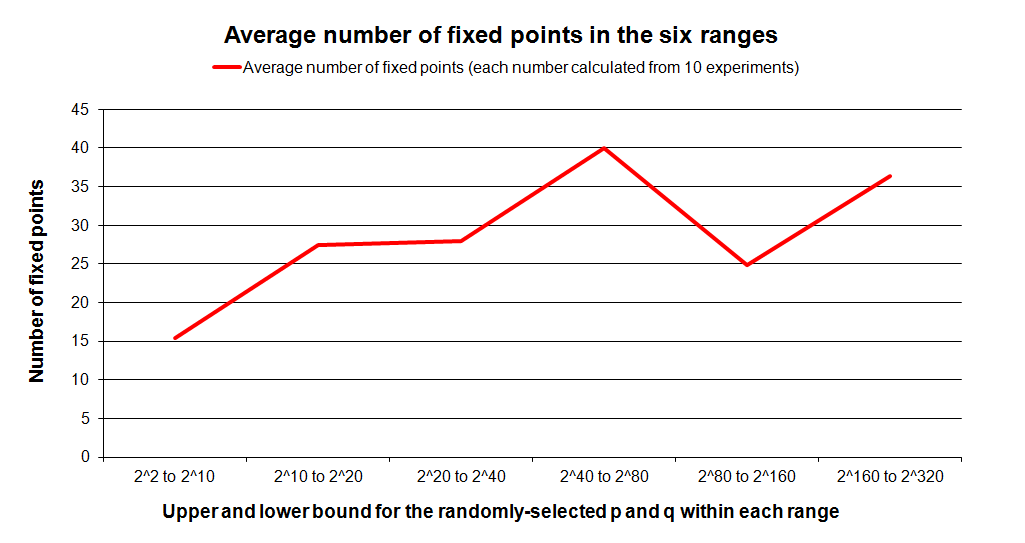
\includegraphics[width=0.92\textwidth]{figures/MAF.png}
  \caption{An empirical estimate of the quantity of fixed points for growing moduli}
  \label{fig:NumberFixpointsGrowingN}
  %\vskip +45pt
\end{figure}

Figure \ref{fig:NumberFixpointsGrowingN} shows that within the six ranges of size,
the average number of fixed points was not higher than 40.
% Unfortunately, we were unable to test the moduli for even higher ranges because 
% our Sage Program \ref{nt_sagesample_Calculate_RSA-Fixpoints}  "`Getfixpoints"'
% was too slow in ranges with $(p,q) > 2^{320}$.\\



\vspace{15pt}
% ----------------------------------------------------
\subsubsection{Example: Determining all fixed points for a specific public RSA key}

The exercise is to determine all fixed points for (n, e) = (866959, 17).\\

\noindent \textbf{Solution:} \\
We start by factoring $n$:  $ 866959 = 811 \cdot 1069$.\\

\noindent The quantity of RSA fixed points results from the theorem
\ref{nt-thm-Anzahl-RSA-Fixpunkte}:\\
$ (gcd(  p-1,  e-1)+1) \cdot (gcd(   q-1,  e-1)+1) =
  (gcd(811-1, 17-1)+1) \cdot (gcd(1069-1, 17-1)+1) = (2+1) \cdot (4+1) = 15 $\\

\noindent Sage program \ref{nt_sagesample_Calculate_RSA-Fixpoints} ``Getfixpoints''
returns the following 15 fixed points for $ (n,e) = (866959, 17)$:
\begin{table}[ht]
\begin{center}
{\tt 
\begin{tabular}{llllllll}
     0 &      1 &  23518 &  23519 &  47037 \\
188964 & 212482 & 236000 & 654477 & 843440 \\
843441 & 630959 & 677995 & 819922 & 866958 
\end{tabular} } % tt
\end{center}
\end{table}

\noindent \textbf{Example:} \\
Using $ 843441$ as a sample for validation:~~
$843441^{17} \mod 866959 = 843441$\\
So $ m = 843441$ is actually a fixed point for the given $(n,e)$.\\

\begin{sagecode}
\begin{Verbatim}%
[fontsize=\footnotesize,fontshape=tt]
import numpy

print "--- Search for fixpoints in Textbook-RSA given p, q, e ---";
fp=numpy.array([0])
fq=numpy.array([0])

#Edit e,p,q here
###EDIT BEGIN###
e=17;
p=811;
q=1069;
###EDIT END###

n=p*q;
print "Prime p: ",p;
print "Prime q: ",q;
print "Modul n: ",n;
print "Public exponent e: ", e;

r=Integers(p)
gen_f_p = r.multiplicative_generator(); print "\nGenerator of f_p: ",gen_f_p;
s=Integers(q)
gen_f_q = s.multiplicative_generator(); print "Generator of f_q: ",gen_f_q;

gcd_p = gcd(e-1,p-1)
gcd_q = gcd(e-1,q-1)
print "\ngcd(e-1,p-1): ", gcd_p;
print "gcd(e-1,q-1): ", gcd_q;

print "\nNumber of fixpoints: ",(gcd_p+1)*(gcd_q+1);
#Calculating fixpoints modulo F_p
#run i from 0 until gcd(e-1,p-1):
#g^( i*(p-1) / (gcd(e-1,p-1)) ) mod p

print "\nFixpoints modulo p";
print "0 (trivial fixpoint added manually)";
i=0;
for i in range(gcd_p):
                fix_p = power_mod(gen_f_p,Integer(i*(p-1)/gcd_p),p); print fix_p;
                fp = numpy.append(fp,fix_p)

print "\nFixpoints modulo q";
print "0 (trivial fixpoint added manually)";
j=0;
for j in range(gcd_q):
                fix_q = power_mod(gen_f_q,Integer(j*(q-1)/gcd_q),q); print fix_q;
                fq = numpy.append(fq,fix_q);

print "\nFixpoints for the public RSA key (n,e) = (", n, ",", e, ")"
for r in fp:
       for s in fq:
               print crt(Integer(r),Integer(s),Integer(p),Integer(q))

print "\nRemark: You can verify each fixpoint with power_mod(m,e,n).";
\end{Verbatim}
\caption{Determining all fixed points for a specific public RSA key}
\label{nt_sagesample_Calculate_RSA-Fixpoints}
\end{sagecode}
%#print "        Here done for the last found fixpoint:";
%#m = crt(Integer(r),Integer(s),Integer(p),Integer(q))
%#print "        m = ", m, ",", "power_mod = ", power_mod(m,e,n)
%#if (m != power_mod(m,e,n)):
%#                print "Verification failed !!!";


\vspace{60pt}
\noindent \textbf{Meaning of the Variables in the Sage Code
                  \ref{nt_sagesample_Calculate_RSA-Fixpoints}:}
\begin{Verbatim}%
[fontsize=\footnotesize,fontshape=tt]
- gen_f_p = r.multiplicative_generator()
  r is a residue class ring modulo p and multiplicative_generator() returns
  a generator element that was created by the ring modulo p.
- power_mod(gen_f_p,Integer(i*(p-1)/gcd_p),p)
  The power_mod function raises a number m to the power of e and returns the results modulo n.
  E.g.: power_mod(m, e, n) := m^e modulo n
- numpy.append(fp,power_mod(gen_f_p,Integer(i*(p-1)/gcd_p),p))
  The append function extends an array (fp) by an additional element.
- crt(Integer(r),Integer(s),Integer(p),Integer(q))
  CRT is the acronym for Chinese Remainder Theorem. crt(r, s, p, q) solves
  the congruences x = r mod p and x = s mod q with the help of the Chinese Remainder Theorem.
\end{Verbatim}

%%% xxx111222xxx-end




% ++++++++++++++++++++++++++++++++++++++++++++++++++++++++++++++++++++++++++
\newpage
\hypertarget{NumberTheory_Appendix_F}{}  %\hypertarget{AppendixListAndDef}{}
\section{Appendix: List of the definitions and theorems formulated in this chapter}
\label{l:NumberTheory_Appendix_F}{}  %\label{l:AppendixListAndDef}{}

\begin{center}
\begin{tabular}{|l|l|l|}\hline
 & Short description ~~ & Page \\ \hline

Definition~\ref{def-zth-prime} & prime numbers &  \pageref{def-zth-prime} \\
Definition~\ref{def-zth-composite} & composite numbers & \pageref{def-zth-composite}  \\ \hline

Theorem~\ref{thm-zth-cnum} & factors of composite numbers~~~~~~~ & \pageref{thm-zth-cnum}\\
Theorem~\ref{thm-zth-mthm} &  1st fundamental theorem of number theory &  \pageref{thm-zth-mthm} \\  \hline

Definition~\ref{def-zth-divisibility} & divisibility & \pageref{def-zth-divisibility} \\
Definition~\ref{def-zth-remainder} & remainder class $r$ modulo $m$ & \pageref{def-zth-remainder} \\
Definition~\ref{def-zth-congruence} & congruent & \pageref{def-zth-congruence} \\ \hline

Theorem~\ref{thm-zth-div} & congruence with difference  & \pageref{thm-zth-div} \\
Theorem~\ref{thm-zth-multinv} & multiplicative inverse (existence) & \pageref{thm-zth-multinv}  \\
Theorem~\ref{thm-zth-exhperm} & exhaustive permutation & \pageref{thm-zth-exhperm} \\
Theorem~\ref{thm-zth-pot} & power mod $m$ & \pageref{thm-zth-pot} \\ \hline

Definition~\ref{def-zth-zn} & $\mathbb{Z}_n$  & \pageref{def-zth-zn}\\
Definition~\ref{def-zth-znmult} &   $\mathbb{Z}_n^*$ & \pageref{def-zth-znmult} \\ \hline

Theorem~\ref{thm-zth-znmult} & multiplicative inverse in $\mathbb{Z}_n^*$& \pageref{thm-zth-znmult} \\ \hline

Definition~\ref{def-zth-phiofn} & Euler function $J(n)$ & \pageref{def-zth-phiofn} \\
Theorem~\ref{thm-zth-phiprime} & $J(p)$ &  \pageref{thm-zth-phiprime}\\
Theorem~\ref{thm-zth-phipq} & $J(p*q)$ &  \pageref{thm-zth-phipq}\\
Theorem~\ref{thm-zth-phimultprime} & $J(p_1 * \cdots *p_k)$ & \pageref{thm-zth-phimultprime} \\
Theorem~\ref{thm-zth-phinum} & $J(p_1^{e_1} * \cdots *p_k^{e_k})$ & \pageref{thm-zth-phinum} \\
Theorem~\ref{thm-zth-fermat1} & little Fermat  &  \pageref{thm-zth-fermat1}\\
Theorem~\ref{thm-zth-fermateuler} & Euler-Fermat theorem & \pageref{thm-zth-fermateuler} \\ \hline

Definition~\ref{def-zth-ordn} & multiplicative order $ {\rm ord}_{m} (a)$ & \pageref{def-zth-ordn} \\
Definition~\ref{def-zth-primitiveroot} & primitive root of $m$ &  \pageref{def-zth-primitiveroot}\\
Theorem~\ref{thm-zth-ordp} & exhausting of all possible values & \pageref{thm-zth-ordp} \\ \hline

Theorem~\ref{nt-thm-Anzahl-RSA-Fixpunkte} & number of RSA fixed points & \pageref{nt-thm-Anzahl-RSA-Fixpunkte} \\ \hline

\end{tabular}
\end{center}
\vskip +6 pt





% ++++++++++++++++++++++++++++++++++++++++++++++++++++++++++++++++++++++++++
% ++++++++++++++++++++++++++++++++++++++++++++++++++++++++++++++++++++++++++
\newpage
\begin{thebibliography}{99999}
\addcontentsline{toc}{section}{Bibliography}

\bibitem[Agrawal2002]{nt:Agrawal2002}  \index{Agrawal 2002} 
    M. Agrawal, N. Kayal, N. Saxena, \\
    {\em PRIMES in P}, August 2002, revised paper: \\
       \url{http://www.cse.iitk.ac.in/~manindra/algebra/primality_v6.pdf}\\
    See also the website "The AKS "PRIMES in P" Algorithm Resource":\\
       \url{http://fatphil.org/maths/AKS/}.
 
\bibitem[Bartholome1996]{nt:3Bartholome1996}  \index{Bartholome 1996} 
    A. Bartholome, J. Rung, H. Kern, \\
    {\em Zahlentheorie f\"ur Einsteiger}, Vieweg 1995, 2nd edition 1996.

\bibitem[Bauer1995]{nt:Bauer1995} \index{Bauer 1995}
    Friedrich L. Bauer, \\
    {\em Entzifferte Geheimnisse}, Springer, 1995.

\bibitem[Bauer2000]{nt:Bauer2000} \index{Bauer 2000}
    Friedrich L. Bauer, \\
    {\em Decrypted Secrets}, Springer 1997, 2nd edition 2000.

\bibitem[Bernstein2001]{nt:Bernstein2001} \index{Bernstein 2001}
    D.~J. Bernstein, \\
    {\em Circuits for integer factorization: a proposal},\\ 
    \url{http://cr.yp.to/papers/nfscircuit.ps} \\
    \url{http://cr.yp.to/djb.html}.

\bibitem[Bernstein2005]{nt:Bernstein2005} \index{ Bernstein 2005}
	Daniel J. Bernstein, \\
	{\em Factoring into coprimes in essentially linear time}, \\
	In Journal of Algorithms 54 (2005), 2005,
	\url{http://cr.yp.to/lineartime/dcba-20040404.pdf}.

\bibitem[Beutelspacher1996]{nt:Beutelspacher1996} \index{Beutelspacher 1996}
    Albrecht Beutelspacher, \\
    {\em Kryptologie}, Vieweg 1987, 5th edition 1996.

\bibitem[Bourseau2002]{nt:Bourseau2002} \index{Bourseau 2002} \index{Fox 2002}
    F. Bourseau, D. Fox, C. Thiel, \\
    {\em Vorz\"uge und Grenzen des RSA-Verfahrens},\\
    In: Datenschutz und Datensicherheit (DuD) 26/2002, pp~84-89 (see www.dud.de),\\
    \url{http://www.secorvo.de/publikationen/rsa-grenzen-fox-2002.pdf}.

\bibitem[Brands2002]{nt:Brands2002} \index{Brands 2002}
    Gilbert Brands, \\
    {\em Verschl\"usselungsalgorithmen -- Angewandte Zahlentheorie 
    rund um Sicherheitsprotokolle}, Vieweg, 2002.

\bibitem[Buchmann2004]{nt:Buchmann2004} \index{Buchmann 2004}
    Johannes Buchmann, \\
    {\em Introduction to Cryptography}, Springer, 2nd edition, 2004.

\bibitem[Buhler1993]{nt:Buhler1993} \index{Buhler 1993} 
    J.P. Buhler, H.W. Lenstra, C. Pomerance, \\
    {\em Factoring integers with the number field sieve}, \\
    In: A.K. Lenstra, H.W. Lenstra (Hrsg.): The Development of the 
    Number Field Sieve, Lecture Notes in Mathematics, vol.~1554, 
    Springer, Heidelberg 1993, pp~50$-$94.

\bibitem[Eckert2003]{nt:Eckert2003} \index{Eckert 2003}
    Claudia Eckert, \\
    {\em IT-Sicherheit: Konzepte-Verfahren-Protokolle}, 
    Oldenbourg 2001, 2nd edition 2003.

\bibitem[Ertel2001]{nt:Ertel2001} \index{Ertel 2001} 
    Wolfgang Ertel, \\
    {\em Angewandte Kryptographie}, 
    Fachbuchverlag Leipzig FV 2001.

\bibitem[Esslinger2012]{nt:Esslinger2012} \index{ Esslinger 2012}
	Esslinger, Schneider, and Simon, \\
	{\em RSA -- Sicherheit in der Praxis }, \\
	in KES -- Zeitschrift f�r Informationssicherheit,
	April 2012.


\bibitem[GISA2012]{nt:GISA2012} \index{GISA 2012}
    GISA (German Information Security Agency), \\
    {\em Recommendation for key length selection}, \\
    \url{https://www.bsi.bund.de/DE/Themen/weitereThemen/ElektronischeSignatur/TechnischeRealisierung/Kryptoalgorithmen/kryptoalgorithmen_node.html}

    BNetzA (Federal Network Agency),\\
    {\em Anually published document about algorithms and their parameters
         in the area of electronic signatures}\\
    \url{http://www.bundesnetzagentur.de/DE/Sachgebiete/QES/Veroeffentlichungen/Algorithmen/algorithmen_node.html}

    A statement on these recommendations: \\
    % \hspace*{1cm}
    \url{http://www.secorvo.de/publikationen/stellungnahme-algorithmenempfehlung-020307.pdf}.


\bibitem[Graham1994]{nt:Graham1994} \index{Graham 1994}
    Graham, Knuth, Patashnik, \\
    {\em Concrete Mathemathics, a Foundation of Computer Science}, \\
    Addison Wesley 1989, 6th printing 1994.

\bibitem[Heninger2012]{nt:Heninger2012} \index{ Heninger 2012}
	Nadia Heninger, Zakir Durumeric, Eric Wustrow, and J. Alex Halderman, \\
	{\em Mining Your Ps and Qs: Detection of Widespread Weak Keys in
        Network Devices }, \\
	August 2012, \url{https://factorable.net/paper.html}.

\bibitem[Katzenbeisser2001]{nt:Katzenbeisser2001} \index{Katzenbeisser 2001}
     Stefan Katzenbeisser, \\
     {\em Recent Advances in RSA Cryptography}, \\
     Springer 2001.

\bibitem[Kippenhahn1997]{nt:Kippenhahn1997} \index{Kippenhahn 1997}
    Rudolph Kippenhahn, \\
    {\em Verschl\"usselte Botschaften -- Geheimschrift, Enigma und Chipkarte}, 
    Rowohlt, 1997.

\bibitem[Kippenhahn1999]{nt:Kippenhahn1999} \index{Kippenhahn 1999}
    Rudolph Kippenhahn, \\
    {\em Code Breaking -- A History and Exploration}, 
    Constable, 1999.
 
\bibitem[Kleinjung2010]{nt:Kleinjung2010} \index{Kleinjung 2010}
    Thorsten Kleinjung et al.\\
    {\em Factorization of a 768-bit RSA modulus},\\
    \url{http://eprint.iacr.org/2010/006.pdf}.

\bibitem[Knuth1998]{nt:Knuth1998} \index{Knuth 1998}
    Donald E. Knuth, \\
    {\em The Art of Computer Programming, vol 2: Seminumerical Algorithms}, \\
    Addison-Wesley, 2nd edition 1998.
    % wann war erste Edition ?

\bibitem[Lenstra1993]{nt:Lenstra1993} \index{Lenstra 1993}
     A. Lenstra, H. Lenstra: \\ 
     {\em The development of the Number Field Sieve}, \\
     Lecture Notes in Mathematics 1554, Springer, New York 1993

\bibitem[Lenstra1999]{nt:Lenstra1999} Arjen K. Lenstra, Eric R. Verheul
     \index{Lenstra/Verheul 1999} \\
     {\em Selecting Cryptographic Key Sizes (1999)},\\
     Journal of Cryptology: the journal of the International 
     Association for Cryptologic Research, \\
     \url{http://www.cryptosavvy.com/cryptosizes.pdf}.
 
\bibitem[Lenstra2002]{nt:Lenstra2002} \index{Lenstra 2002}
    Arjen K. Lenstra, Adi Shamir, Jim Tomlinson, Eran Tromer,\\
    {\em Analysis of Bernstein's Factorization Circuit},\\
    \url{http://www.cryptosavvy.com/mesh.pdf}.

\bibitem[Lenstra2012]{nt:Lenstra2012} \index{ Lenstra 2012}
	Arjen K. Lenstra, James P. Hughes, Maxime Augier, Joppe W. Bos,
        Thorsten Kleinjung and Christophe Wachter, \\
	{\em Ron was wrong, Whit is right, A Sanity Check of Public Keys
             Collected on the Web}, \\
	February 2012,
	\url{http://eprint.iacr.org/2012/064.pdf}.

\bibitem[Menezes2001]{nt:Menezes2001} \index{Menezes 2001}
    Alfred J. Menezes, Paul C. van Oorschot, Scott A. Vanstone \\
    {\em Handbook of Applied Cryptography}, 
    CRC Press 1997, 5th printing 2001,\\
    \url{http://www.cacr.math.uwaterloo.ca/hac/} (Errata last updated July 24, 2011).

\bibitem[Oechslin2003]{nt:Oechslin2003} \index{ Oechslin 2003}
	Philippe Oechslin,\\
	{\em Making a Faster Cryptanalytic Time-Memory Trade-Off},\\
	At Crypto 2003, 2003,\\
	\url{http://lasecwww.epfl.ch/pub/lasec/doc/Oech03.pdf}.

\bibitem[Pfleeger1997]{nt:Pfleeger1997} \index{Pfleeger 1997}
    Charles P. Pfleeger, \\
    {\em Security in Computing}, Prentice-Hall, 2nd edition 1997.
    % im Buch stand nicht, wann die 1. Edition rauskam.

\bibitem[Pomerance1984]{nt:Pomerance1984} \index{Pomerance 1984} 
    C. Pomerance, \\
    {\em The quadratic sieve factoring algorithm}, \\
    In: G.R. Blakley, D. Chaum (Hrsg.): Proceedings of Crypto '84, 
    LNCS 196, Springer Berlin 1995, pp~169-182.

\bibitem[RSA Security 2002]{nt:RSA Security 2002} \index{RSA Security 2002} 
    RSA Security, \\
    {\em Has the RSA algorithm been compromised as a result 
    of Bernstein's Paper?}, \\
    April 8th, 2002, \\
    \url{http://www.rsasecurity.com/}.
     
\bibitem[SchneiderM2004]{nt:SchneiderM2004} \index{SchneiderM 2004} 
    Matthias Schneider, \\
    {\em Analyse der Sicherheit des RSA-Algorithmus. \\
     M\"ogliche Angriffe, deren Einfluss auf sichere Implementierungen und \"okonomische Konsequenzen}, \\
    Diploma thesis at the University of Siegen, Germany, 2004.

\bibitem[Schneier1996]{nt:Schneier1996nt} \index{Schneier 1996} 
    Bruce Schneier, \\
    {\em Applied Cryptography, Protocols, Algorithms, and Source Code in C}, \\
    Wiley and Sons, 2nd edition 1996.

\bibitem[Schulz2010]{nt:Schulz2010} \index{Schulz 2010}%\index{Time experiments}
    R.-H. Schulz, Helmut Witten, \\
    {\em Zeitexperimente zur Faktorisierung. Ein Beitrag zur Didaktik
         der Kryptographie}, 
    LogIn, no. 166/167, 2010, pp~113-120\\
    \url{http://bscw.schule.de/pub/bscw.cgi/d864899/Schulz_Witten_Zeit-Experimente.pdf}.

\bibitem[Schwenk2002]{nt:Schwenk2002}\index{Schwenk 2002}
    J\"org Schwenk, \\
    {\em Sicherheit und Kryptographie im Internet}, 
    Vieweg 2002.

\bibitem[Sedgewick1990]{nt:Sedgewick1990} \index{Sedgewick 1990}
    Robert Sedgewick,\\
    {\em Algorithms in C}, Addison-Wesley, 1990.

\bibitem[Shamir2003]{nt:Shamir2003} \index{Shamir 2003} \index{TWIRL device} 
    Adi Shamir, Eran Tromer, \\
    {\em Factoring Large Numbers with the TWIRL Device}, 
    Januar 2003, \\
    \url{http://www.wisdom.weizmann.ac.il/~tromer/}.

\bibitem[Shamir2003a]{nt:Shamir2003a} \index{Shamir 2003a} \index{TWIRL device} 
    Adi Shamir, Eran Tromer, \\
    {\em On the Cost of Factoring RSA-1024}, 
    RSA Laboratories CryptoBytes volume 6, no. 2, Summer 2003, pp~11-20, \\
    \url{http://www.rsasecurity.com/rsalabs/cryptobytes/CryptoBytes_August_2003.pdf}

\bibitem[Silverman2000]{nt:Silverman2000} \index{Silverman 2000}
     Robert D. Silverman: \\ 
     {\em A Cost-Based Security Analysis of Symmetric and Asymmetric 
          Key Lengths} \\
     In: RSA Laboratories Bulletin, no. 13, April 2000, pp~1-22

\bibitem[Stinson1995]{nt:Stinson1995} \index{Stinson 1995}
    Douglas R. Stinson,\\
    {\em Cryptography - Theory and Practice}, CRC Press, 1995.

\bibitem[Weis2003]{nt:Weis2003} \index{Weis 2003} \index{Lucks 2003} \index{Bogk 2003}
    R\"udiger Weis, Stefan Lucks, Andreas Bogk, \\
    {\em Sicherheit von 1024 bit RSA-Schl\"usseln gef\"ahrdet},\\
    In: Datenschutz und Datensicherheit (DuD) 6/2003, pp~360-362 (see www.dud.de)\\
    The article explains details about the TWIRL device\index{TWIRL device}.

\bibitem[Welschenbach2001]{nt:Welschenbach2001} \index{Welschenbach 2001}
    Welschenbach, Michael, \\
    {\em Kryptographie in C und C++}, Springer 2001.
    
\bibitem[Wiles1994]{nt:Wiles1994} \index{Wiles, Andrew}
    Wiles, Andrew, \\
    {\em Modular elliptic curves and Fermat's Last Theorem}, 
    \index{Fermat!last theorem} \\
    In: Annals of Mathematics 141 (1995).

\bibitem[Wolfenstetter1998]{nt:Wolfenstetter1998} \index{Wolfenstetter 1998}
    Albrecht Beutelspacher, J\"org Schwenk, Klaus-Dieter Wolfenstetter, \\
    {\em Moderne Verfahren in der Kryptographie}, 
    Vieweg 1995, 2nd edition 1998.

\bibitem[Yan2000]{nt:Yan2000} \index{Yan 2000} 
    Song Y. Yan, \\
    {\em Number Theory for Computing}, Springer, 2000.
\end{thebibliography}



% ++++++++++++++++++++++++++++++++++++++++++++++++++++++++++++++++++++++++++
\newpage
\section*{Web links}
\addcontentsline{toc}{section}{Web links}

\begin{enumerate}
   \item \hypertarget{knott}{}  \index{Knott, Ron}
         Ron Knott's Fibonacci \index{Fibonacci} page, \\
         Here, everything revolves around Fibonacci numbers.\\
          \url{http://www.mcs.surrey.ac.uk/personal/R.Knott/Fibonacci/fib.html}
          
   \item CrypTool, \index{CrypTool} \\
         Open source e-learning software to illustrate cryptography and
         cryptanalysis\\
          \url{http://www.cryptool.de}, \\
          \url{http://www.cryptool.org},\\ 
          \url{http://www.cryptool.com}
          
   \item Mathematica, \index{Mathematica} \\
         Commercial mathematics package \\
         \url{http://www.wolfram.com}
          
   \item LiDIA, \index{LiDIA} \\
         Extensive library containing number-theory functions and the
         LC interpreter. Maintenance stopped. \\
          \url{http://www.informatik.tu-darmstadt.de/TI/LiDIA}
          
   \item BC, \index{BC} \\
         Interpreter with number-theory functions \\
         \url{http://www.gnu.org/software/bc/bc.html}
          
   \item Pari-GP, \index{Pari-GP} \\
         Excellent, fast, free interpreter with number theoretical functions.\\
         \url{http://pari.math.u-bordeaux.fr/} \\
         \url{http://en.wikipedia.org/wiki/PARI/GP} \\
         Resources for PARI/GP at Karim Belabas's website:\\
         \url{http://www.math.u-bordeaux.fr/~belabas/pari/}
           
   \item \index{Munchenbach@M\"unchenbach, Carsten}
         Only after I had completed this article, did I come across the
         website of Mr.\ M\"unchenbach, which interactively and didactically
         uses elementary number theory to provide a sophisticated
         description of the fundamental mathematical thought processes. 
         It was created for a teaching project in the 11th grade of the
         technical grammar school (unfortunately only available in German): \\
         \url{http://www.hydrargyrum.de/kryptographie}
                      
   \item Web site of Mr.~Wagner, who is responsible for the development
	 of the curriculum of computer science in one of the German federal 
         states (L\"ander). Here you can get hold of a collection of texts
	 and (Java-)\discretionary{}{}{}programs (available only in German):\\
         \url{http://www.saar.de/~awa/kryptolo.htm}
          
   \item GISA, \index{GISA} \\
         German Information Security Agency \\
         \url{http://www.bsi.bund.de}

   \item Factorization records and challenges\index{Factorization!factoring records},\\
         \url{http://www.crypto-world.com/} \\
         \url{http://www.crypto-world.com/FactorWorld.html}, Webseite von Scott Contini \\
         \url{http://www.loria.fr/~zimmerma/records/factor.html} \\

         \url{http://www.tutorgig.com/ed/RSA\_number} \\

         \url{http://www.uni-bonn.de/Aktuelles/Pressemitteilungen/pm02/pm035-02.html} \\
         \url{http://www.ercim.org/publication/Ercim\_News/enw49/franke.html} \\ %2002-01
         \url{http://www.loria.fr/~zimmerma/records/rsa160} \\

         \url{http://www.rsa.com/rsalabs/node.asp?id=2092}
	 

   \item The Cunningham Project, \index{Cunningham project}\\ 
         \url{http://www.cerias.purdue.edu/homes/ssw/cun/}


   \item Sage, \index{Sage} \\
         Excellent, open source computer algebra system with Python as script
         language, used to build the code samples in this chapter.
	 See the introduction in chapter~\ref{s:appendix-using-sage}.\\
         \url{http://www.sagemath.org/} \\
         \url{http://en.wikipedia.org/wiki/Sage_%28mathematics_software%29}

\end{enumerate}



% ++++++++++++++++++++++++++++++++++++++++++++++++++++++++++++++++++++++++++
\vskip +20 pt
\section*{Acknowledgments}
\addcontentsline{toc}{section}{Acknowledgments}

I would like to take this opportunity to thank 
\begin{itemize}

  \item {Henrik Koy for making many very useful suggestions, 
         for the very constructive proof-reading of the first version of
	 this article, and for helping with TeX.}

  \item {J\"org Cornelius Schneider for his enthusiastic TeX support and for the
         many cases where he helped when facing programming or design problems.}
  
  \item {Dr.\ Georg Illies for pointing me to Pari-GP\index{Pari-GP}.}
  
  \item {Lars Fischer for his help with fast Pari-GP\index{Pari-GP} code for
        primitive roots.}
  
  \item {Minh Van Nguyen from Australia for his always fast, professional and exhaustive
         help with the first Sage\index{Sage} code samples in this chapter.}

\end{itemize}



% Local Variables:
% TeX-master: "../script-en.tex"
% End:

% $Id$
\setcounter{satz}{0}
\setcounter{definition}{0}

\newcommand{\NT}{\vspace*{0.2\baselineskip}\\}
\newcommand{\HZ}{\vspace*{0.5\baselineskip}}
\newcommand{\R}{\text{I}\!\text{R}}
\newcommand{\N}{\text{I}\!\text{N}}
\newcommand{\Q}{\text{Q}\!\!\!\text{l}\,\,}
\newcommand{\C}{\text{C}\!\!\!\text{l}\,\,}
\newcommand{\K}{\text{I}\!\text{K}}
\newcommand{\Z}{\mathbf{\mathbb{Z}}}
%--------------------------------------- matheScript-Zeichen definieren
\newcommand{\fs}{\mathscr{F}}  
\newcommand{\es}{\mathscr{E}}  
\newcommand{\cs}{\mathscr{C}}  
\newcommand{\gs}{\mathscr{G}}
\newcommand{\is}{\mathscr{I}}
\newcommand{\os}{\mathscr{O}}
\newcommand{\ks}{\mathscr{K}}
\newcommand{\qs}{\mathscr{Q}}
\newcommand{\us}{\mathscr{U}}
\newcommand{\hs}{\mathscr{H}}
\newcommand{\ps}{\mathscr{P}}
\newcommand{\as}{\mathscr{A}}
\newcommand{\rs}{\mathscr{R}}
\newcommand{\bs}{\mathscr{B}}
%-------------------------------------
\newcommand{\PG}{\text{I}\!\text{P}}
\newcommand{\carre}{\square}
\newcommand{\ncarre}{/\negthickspace\negthickspace\square}
\newcommand{\ncarreq}{{\ncarre}_q}
\newcommand{\ncarree}{/\negthickspace\negthickspace\negthickspace\square}
\newcommand{\ncarrepi}{{\ncarre}_{p^i}}
\newcommand{\mc}[1]{{\cal #1}}
\newcommand{\Char}{\text{char}}
\newcommand{\Aut}{\text{Aut}}
\newcommand{\Fix}{\text{Fix}}
\newcommand{\Syl}{\text{Syl}}
\newcommand{\Bild}{\text{Bild}}
\newcommand{\ggt}{\text{ggT}}
\newcommand{\kgv}{\text{kgV}}
\newcommand{\Id}{\text{Id}}
\newcommand{\nqcarre}{{\ncarre}_{q^2}}

\setlength{\fboxrule}{.4pt}
\setlength{\fboxsep}{4pt}


\newpage
%********************************************************************
\hypertarget{Chapter_ModernCryptography}{}
\chapter[Die mathematischen Ideen hinter der modernen Kryptographie]
        {Die mathematischen Ideen hinter der modernen Kryptographie\footnotemark}
\footnotetext{%
    \index{ZT, Lernprogramm Zahlentheorie}%
    \index{Lernprogramm ZT}%
    Mit dem Lernprogramm {\bf ZT} k�nnen Sie spielerisch einige der hier
    besprochenen Verfahren (RSA, Rabin, DH, ElGamal) nachvollziehen
    (siehe Lern-Kapitel 4.2 und 4.3, Seiten 9-17/17).\\
    ZT k�nnen Sie in CrypTool\index{CrypTool} �ber das Men�
    {\bf Einzelverfahren \textbackslash{} Zahlentheorie 
    interaktiv \textbackslash{} Lernprogramm f�r Zahlentheorie} aufrufen.
    Siehe Anhang \ref{s:appendix-Learn-NT}.
}
\label{Chapter_ModernCryptography}
%********************************************************************
(Oyono R./ Esslinger B./ Schneider J., Sep. 2000;
           Updates Nov. 2000, Feb. 2003, Apr. 2007, M�rz 2010)


\vskip +30 pt

\begin{center}
\fbox{\parbox{15cm}{
   {\em Georg Christoph Lichtenberg\footnotemark:}\\
   Ich wei� nicht, ob es besser wird, wenn wir es �ndern,\\
   aber ich wei�, dass wir es �ndern m�ssen, wenn es besser werden soll.\\

   {\em Anmerkung von Unbekannt (Radio) dazu:}\\
   Und Gott gebe den Akteuren bei der notwendigen Umsetzung\\
   das Wissen, die Weisheit und das Verantwortungsbewusstsein,\\
   zwischen Aktionismus, Selbstdarstellung und planvollem Handeln\\
   zu unterscheiden -- und ihr Wissen auch anzuwenden.
}}
\end{center}
\footnotetext{%
  Georg Christoph Lichtenberg\index{Lichtenberg, Georg Christoph}, 
  deutscher Schriftsteller und Physiker (1742-1799),\\ 
  (siehe auch: \href{http://de.wikipedia.org/wiki/Georg\_Christoph\_Lichtenberg}
                {\tt http://de.wikipedia.org/wiki/Georg\_Christoph\_Lichtenberg})
}

%--------------------------------------------------------------------
\hypertarget{OneWayFunktion1}{}
\section{Einwegfunktionen mit Fallt�r und Komplexit�tsklassen}
\label{OneWayFunktion1}
%--------------------------------------------------------------------
\index{Kryptographie!moderne} \index{Einwegfunktion}
Eine {\bf Einwegfunktion} ist eine effizient zu 
berechnende Funktion, deren Umkehrung jedoch nur mit 
extrem hohem Rechenaufwand -- jedoch praktisch unm�glich -- zu berechnen ist.\par

Etwas genauer formuliert:  Eine Einwegfunktion ist eine Abbildung $ f $ einer Menge $ X $ in eine Menge $ Y, $ so dass $ f(x) $ f�r jedes Element $ x $ von $ X $ leicht zu berechnen ist, w�hrend es f�r (fast) jedes $ y $ aus $ Y $  praktisch unm�glich ist, ein Urbild $ x $ (d.h. ein $ x $ mit $ f(x)=y $) zu finden.\par

Ein allt�gliches Beispiel f�r eine Einwegfunktion ist ein Telefonbuch: die auszuf�hrende Funktion ist die, einem Namen die entsprechende Telefonnummer zuzuordnen. Da die Namen alphabetisch geordnet sind, ist diese Zuordnung einfach auszuf�hren. Aber ihre Invertierung, also die Zuordnung eines Namens zu einer gegebenen Nummer, ist offensichtlich schwierig, wenn man nur ein Telefonbuch zur Verf�gung hat. \par

Einwegfunktionen spielen in der Kryptographie eine entscheidende Rolle. Fast alle kryptographischen Begriffe kann man durch Verwendung des Begriffs Einwegfunktion umformulieren. Als Beispiel betrachten wir die Public-Key-Verschl�sselung \index{Verschl�sselung!Public-Key} (asymmetrische Kryptographie):\par

Jedem Teilnehmer $ T $ des Systems wird ein privater \index{Schl�ssel!privat}
\index{Schl�ssel!�ffentlich} Schl�ssel $d_T$~\mbox{und} ein sogenannter �ffentlicher Schl�ssel $ e_T $   zugeordnet. Dabei muss die folgende Eigenschaft (Public-Key-Eigen"-schaft) gelten:\\
F�r einen Gegner, der den �ffentlichen Schl�ssel $ e_T $  kennt, ist es praktisch unm�glich, den privaten Schl�ssel  $ d_T $ zu bestimmen.\par

Zur Konstruktion n�tzlicher Public-Key-Verfahren sucht man also eine Einwegfunktion, die in einer Richtung \glqq einfach\grqq {} zu berechnen, die in der anderen Richtung jedoch \glqq schwer\grqq {} (praktisch unm�glich) zu berechnen ist, solange eine bestimmte zus�tzliche Information \index{Einwegfunktion!mit Fallt�r} (Fallt�r) nicht zur Verf�gung steht. Mit der zus�tzlichen Information kann die Umkehrung effizient gel�st werden. Solche Funktionen nennt man {\bf Einwegfunktionen mit Fallt�r} (trapdoor one-way function). Im obigen Fall ist $ d_T $ die Fallt�r-In"-for"-ma"-tion. \par

Dabei bezeichnet man ein Problem als \glqq einfach\grqq, wenn es in \index{Laufzeit!polynomial} \index{Polynom} polynomialer Zeit als Funktion der L�nge der Eingabe l�sbar ist, d.h. wenn es so gel�st werden kann, dass der Zeitaufwand sich als polynomiale Funktion in Abh�ngigkeit der L�nge der Eingabe darstellen l�sst. 
Wenn die L�nge der Eingabe $ n $ Bits betr�gt, so ist die Zeit der Berechnung der Funktion proportional zu $ n^{a}, $ wobei $ a $  eine Konstante ist. Man sagt, dass die \index{Komplexit�t} Komplexit�t solcher Probleme $ O(n^{a}) $ betr�gt (Landau- oder Big-O-Notation). 

Vergleicht man 2 Funktionen  $ 2^n $  und   $ n^{a} $, wobei $ a $  
eine Konstante ist, dann gibt es immer einen Wert f�r  $ n $, ab dem
f�r alle weiteren $ n $ gilt: $ n^{a}  <  2^n $. 
Die Funktion  $ n^{a} $  hat eine geringere Komplexit�t.
Z.B. f�r $ a=5 $ gilt: ab der L�nge $ n=23 $ ist 
$ 2^n > n^5 $ ~\mbox{und} danach w�chst $ 2^n $ auch deutlich 
schneller \
[($ 2^{22}= 4.194.304 $, $ 22^5= 5.153.632 $), \
 ($ 2^{23}= 8.388.608 $, $ 23^5= 6.436.343 $), \
 ($ 2^{24}=16.777.216 $, $ 24^5= 7.962.624 $)].\par 
% "\mbox" nur, weil bei Ausdruck bei be die Blanks stets falsch sa�en:
%  "n^5un d"

Der Begriff \glqq praktisch unm�glich\grqq {} ist etwas schwammiger. 
Allgemein kann man sagen, ein Problem ist \index{Laufzeit!effizient}
nicht effizient l�sbar, wenn der zu seiner L�sung ben�tigte Aufwand
schneller w�chst als die polynomiale \index{Polynom} Zeit als Funktion der Gr��e der
Eingabe. Wenn beispielsweise die L�nge der Eingabe $ n $  Bits betr�gt
und die Zeit zur Berechnung der Funktion proportional zu $ 2^n $ ist, 
so gilt gegenw�rtig: die Funktion ist f�r $n > 80$ praktisch nicht zu 
berechnen.

Die Entwicklung eines praktisch einsetzbaren Public-Key-Verfahrens h�ngt daher von der Entdeckung einer geeigneten Einwegfunktion mit Fallt�r ab.\par

Um Ordnung in die verwirrende Vielfalt von m�glichen Problemen und ihre Komplexit�ten zu bringen, fasst man Probleme mit �hnlicher Komplexit�t zu Klassen zusammen.

Die wichtigsten Komplexit�tsklassen  sind die Klassen \textbf{P} und \textbf{NP}: 

\begin{itemize}

    \item Die Klasse \textbf{P}: Zu dieser Klasse geh�ren diejenigen Probleme, die mit polynomialem \index{Polynom} Zeitaufwand l�sbar sind.
    
    \item Die Klasse \textbf{NP}: Bei der Definition dieser Klasse betrachten wir nicht den Aufwand zur L�sung eines Problems, sondern den Aufwand zur Verifizierung einer gegebenen L�sung. Die Klasse \textbf{NP} besteht aus denjenigen Problemen, bei denen die Verifizierung einer gegebenen L�sung mit polynomialem Zeitaufwand m�glich ist. Dabei bedeutet der Begriff \textbf{NP} \glqq nichtdeterministisch\grqq {} polynomial \index{Polynom} und bezieht sich auf ein Berechnungsmodell, d.h. auf einen nur in der Theorie existierenden Computer, der richtige L�sungen nichtdeterministisch \glqq raten\grqq {} und dies dann in polynomialer Zeit verifizieren kann.

\end{itemize}

Die Klasse \textbf{P} ist in der Klasse \textbf{NP} enthalten. Ein ber�hmtes offenes Problem ist die Frage, ob $ \textbf{P} \neq \textbf{NP} $ gilt oder nicht, d.h. ob \textbf{P} eine echte Teilmenge ist oder nicht. Eine wichtige Eigenschaft der Klasse \textbf{NP} ist, dass sie auch sogenannte \glqq \textbf{NP}-vollst�ndige\grqq {} Probleme enth�lt. Dies sind Probleme, welche die Klasse \textbf{NP} im Folgenden Sinne vollst�ndig repr�sentieren: Wenn es einen \glqq guten\grqq {} Algorithmus f�r ein solches Problem gibt, dann existieren f�r alle Probleme aus \textbf{NP} \glqq gute\grqq {} Algorithmen. Insbesondere gilt: wenn auch nur ein vollst�ndiges Problem in \textbf{P} l�ge, d.h. wenn es einen polynomialen \index{Polynom} L�sungsalgorithmus f�r dieses Problem g�be, so w�re \textbf{P}=\textbf{NP}. In diesem Sinn sind die \textbf{NP}-vollst�ndigen Probleme die schwierigsten Probleme in \textbf{NP}.

Viele kryptographische Protokolle sind so gemacht, dass die \glqq guten\grqq {} Teilnehmer nur Probleme aus \textbf{P} l�sen m�ssen, w�hrend sich ein Angreifer vor Probleme aus \textbf{NP} gestellt sieht.

Man wei� leider bis heute nicht, ob es Einwegfunktionen �berhaupt gibt. Man kann aber zeigen, dass Einwegfunktionen genau dann existieren, wenn $ \textbf{P} \neq \textbf{NP} $ gilt \cite[S.63]{mc:Balcazar1988}.
\vskip +5pt

Immer wieder behauptete jemand, er habe die �quivalenz bewiesen
(z.B.  \cite{mc:Hesselink2001}), %%Hinweis wegen geocities per he.pa, 16.2.2010
aber bisher erwiesen sich diese Aussagen stets als falsch.

Es wurden eine Reihe von Algorithmen f�r Public-Key-Verfahren vorgeschlagen. Einige davon erwiesen sich, obwohl sie zun�chst vielversprechend erschienen, als polynomial \index{Polynom} l�sbar. Der ber�hmteste durchgefallene Bewerber ist der von Ralph Merkle \cite{mc:Merkle1978} vorgeschlagene Knapsack mit Fallt�r.


%\newpage
\vskip +20 pt
%--------------------------------------------------------------------
\section{Knapsackproblem als Basis f�r Public-Key-Verfahren}
\index{Kryptographie!Public-Key}
%--------------------------------------------------------------------

%--------------------------------------------------------------------
\subsection{Knapsackproblem} \index{Knapsack}

Gegeben $ n $ Gegenst�nde $ G_1, \dots, G_n $ mit den Gewichten $ g_1, \dots g_n $ und den Werten $w_1, \cdots, w_n. $ Man soll wertm��ig so viel wie m�glich unter Beachtung einer oberen Gewichtsschranke $ g $ davontragen. Gesucht ist also eine Teilmenge von $ \{ G_1, \cdots,G_n\}, $ etwa $ \{G_{i_1}, \dots ,G_{i_k} \}, $ so dass  $ w_{i_1}+ \cdots +w_{i_k} $ maximal wird unter der Bedingung $  g_{i_1}+ \cdots +g_{i_k} \leq g. $ \par
Derartige Fragen sind sogenannte {\bf NP}-vollst�ndige Probleme (nicht \index{Laufzeit!nicht polynomial NP} deterministisch polynomial\index{Polynom}), die aufwendig zu berechnen sind.\index{Knapsack}

Ein Spezialfall des Knapsackproblems ist:\\
Gegeben sind die nat�rlichen Zahlen $ a_1, \dots, a_n $   und $ g .$
Gesucht sind  $ x_1, \dots, x_n \in \{ 0,1\} $  mit $ g = \sum_{i=1}^{n}x_i a_i $  (wo also $ g_i = a_i = w_i $ gew�hlt ist).
Dieses Problem hei�t auch  {\bf 0-1-Knapsackprob"-lem} und wird mit $ K(a_1, \dots, a_n;g) $  bezeichnet.\\

Zwei 0-1-Knapsackprobleme  $ K(a_1, \dots, a_n;g) $   und
$ K(a'_1, \dots, a'_n;g') $  hei�en kongruent, falls es zwei
teilerfremde\index{Zahlen!teilerfremde (co-prime)} Zahlen $ w $ und $ m $
gibt, so dass
\begin{enumerate}
    \item $ m > \max \{ \sum_{i=1}^n a_i , \sum_{i=1}^n a'_i \}, $

    \item $ g \equiv wg' \mod m, $

    \item $ a_i \equiv w a'_i \mod m $ f�r alle $ i=1, \dots, n.$

\end{enumerate}
 
\begin{remark}{:}\\
Kongruente 0-1-Knapsackprobleme haben dieselben L�sungen.
Ein schneller Algorithmus zur Kl�rung der Frage, ob zwei 0-1-Knapsackprobleme kongruent sind, ist nicht bekannt.
\end{remark}

Das L�sen eines 0-1-Knapsackproblems kann durch Probieren der $ 2^n $   M�glichkeiten f�r $ x_1, \dots, x_n $   erfolgen. Die beste Methode erfordert $ O(2^{n/2}) $  Operationen, was f�r $ n=100 $  mit $ 2^{100} \approx 1,27 \cdot 10^{30} $  und  $ 2^{n/2} \approx 1,13 \cdot 10^{15} $ f�r Computer eine un�berwindbare H�rde darstellt.
Allerdings ist die L�sung f�r spezielle $ a_1, \dots, a_n $   recht einfach zu finden, etwa f�r $ a_i = 2^{i-1}. $  Die bin�re Darstellung von $ g $ liefert unmittelbar $ x_1, \dots, x_n$. Allgemein ist die L�sung des 0-1-Knapsackproblems leicht zu finden, falls eine \index{Permutation} Permutation\footnote{Eine Permutation\index{Permutation} $\pi$ der Zahlen $1, \dots, n$ ist die Vertauschung der Reihenfolge, in der
diese Zahlen aufgez�hlt werden. Beispielsweise ist eine Permutation $\pi$ von $(1,2,3)$ gleich $(3,1,2),$ also $\pi(1) = 3$, $\pi(2) =1$ 
und $\pi(3) = 2$.} 
$ \pi $  von $ 1, \dots, n $  mit $ a_{\pi (j)} > \sum_{i=1}^{j-1} a_{\pi(i)} $  existiert. Ist zus�tzlich $ \pi $ die Identit�t, d.h. $ \pi(i)=i $ f�r $ i=1,2,\dots,n, $ so hei�t die Folge $ a_1, \dots , a_n $ superwachsend.
Das Verfahren \ref{knapsackalgo} l�st das Knapsackproblem mit superwachsender Folge im Zeitraum von $ O(n). $
\begin{cryptoprocedure}
\begin{tabbing}
\hspace*{0.5cm} \= \hspace*{0.5cm} \= \hspace*{0.5cm} \= \kill
\>{\bf for} $ i=n $ {\bf to} 1 {\bf do} \\
\>\> {\bf if} $ T\geq a_i $ {\bf then}\\
\>\> \> $ T:=T-s_i $ \\
\>\>\> $ x_i:=1 $ \\
\>\> {\bf else} \\
\>\>\> $ x_i:=0 $\\
\>{\bf if} $ T=0 $ {\bf then} \\
\>\> $ X:=(x_1, \dots, x_n) $ ist die L�sung. \\
\>{\bf else} \\
\>\> Es gibt keine L�sung.
\end{tabbing}
\caption{L�sen von Knapsackproblemen mit superwachsenden Gewichten}
\label{knapsackalgo}
\end{cryptoprocedure}


%--------------------------------------------------------------------
\subsection{Merkle-Hellman Knapsack-Verschl�sselung}
\index{Hellman, Martin} \index{Merkle, Ralph} 

1978 gaben Merkle und Hellman \cite{mc:Merkle1978} \index{Verschl�sselung!Merkle-Hellman} ein Public-Key-Verschl�sselungs-Verfahren an, das darauf beruht, das leichte 0-1-Knapsackproblem mit einer superwachsenden Folge in ein kongruentes mit einer nicht superwachsenden Folge zu \glqq verfremden\grqq. Es ist eine Blockchiffrierung, die bei jedem Durchgang einen $n$ Bit langen Klartext chiffriert, siehe Krypto-Verfahren \ref{merklehellmanproc}.
\index{Knapsack!Merkle-Hellman}

\begin{cryptoprocedure}
Es sei $ (a_1, \dots, a_n) $ superwachsend. Seien $ m $ und $ w $ zwei
teilerfremde\index{Zahlen!teilerfremde (co-prime)} Zahlen mit $ m >
\sum_{i=1}^{n} a_i $ und $ 1\leq w \leq m-1. $
W�hle $\bar{w} $ mit $ w \bar{w} \equiv 1 \mod m $ die modulare Inverse
von $ w $ und setze $ b_i:= wa_i \mod m, $ $ 0\leq b_i < m $ f�r $ i=1,
\dots ,n, $ und pr�fe, ob die Folge $ b_1, \dots b_n $ nicht superwachsend
ist. Danach wird eine Permutation $ b_{\pi (1)}, \dots , b_{\pi(n)} $
von $ b_1, \dots , b_n $ publiziert und insgeheim die zu $ \pi $ inverse
Permutation $ \mu $ festgehalten. Ein Sender schreibt seine Nachricht
in Bl�cke $ (x_1^{(j)}, \dots, x_n^{(j)}) $ von Bin�rzahlen der L�nge
$ n $ und bildet \[ g^{(j)}:= \sum_{i=1}^n x_{i}^{(j)} b_{\pi(i)} \]
und sendet $ g^{(j)}, (j=1,2, \dots). $\par
Der Schl�sselinhaber bildet
\[ G^{(j)}:=\bar{w} g^{(j)} \mod m ,\quad 0 \leq G^{(j)} < m \]
und verschafft sich die $ x_{\mu(i)}^{(j)} \in \{ 0,1\} $ (und somit auch die $ x_i^{(j)} $) aus
\begin{eqnarray*}
G^{(j)} & \equiv & \bar{w} g^{(j)} = \sum_{i=1}^n x_i^{(j)} b_{\pi (i)} \bar{w} \equiv \sum_{i=1}^n x_i^{(j)} a_{\pi (i)} \mod m \\
& = & \sum_{i=1}^n x_{\mu (i)}^{(j)} a_{\pi (\mu (i))} = \sum _{i=1}^n x_{\mu (i)}^{(j)} a_i \mod m, 
\end{eqnarray*}
indem er die leichten 0-1-Knapsackprobleme $ K(a_1,\dots,a_n;G^{(j)}) $ mit superwachsender Folge $ a_1, \dots,a_n $ l�st.
\caption{Merkle-Hellman (auf Knapsackproblemen basierend)}
\label{merklehellmanproc}
\end{cryptoprocedure}



1982 gab \index{Shamir, Adi} Shamir \cite{mc:Shamir1982} einen Algorithmus zum
Brechen des Systems in polynomialer \index{Polynom} Zeit an, ohne das allgemeine
Knapsackproblem zu l�sen. Len \index{Adleman, Leonard} Adleman
\cite{mc:Adleman1982} und Jeff Lagarias \index{Lagarias, Jeff}
\cite{mc:Lagarias1983} gaben einen Algorithmus zum Brechen des 2-fachen
iterierten Merkle-Hellman Knapsack-Verschl�sselungsver"-fah"-rens in
polynomialer Zeit an. Ernst Brickell \index{Brickell, Ernst}
\cite{mc:Brickell1985} gab schlie�lich einen Algorithmus zum Brechen des
mehrfachen iterierten Merkle-Hellman Knapsack-Verschl�sselungs"-ver"-fah"-ren in
polynomialer Zeit an. Damit war dieses Verfahren als
Verschl�sse"-lungs"-ver"-fah"-ren ungeeignet. Dieses Verfahren liefert also eine
Einwegfunktion, deren Fallt�r-In"-for"-ma"-tion (Verfremden des
0-1-Knapsackproblems) durch einen Gegner entdeckt werden k�nnte.


%---------------------------------------------------------------------
\section{Primfaktorzerlegung als Basis f�r Public-Key-Verfahren}
\index{Primfaktor!Zerlegung}
%--------------------------------------------------------------------

%--------------------------------------------------------------------
\hypertarget{RSAVerfahren}{}
\subsection[Das RSA-Verfahren]
{Das RSA-Verfahren\footnote{%
Vergleiche auch die Kapitel \ref{rsabeweis}, ff.
}$^,$\footnote{%
Mit CrypTool\index{CrypTool} k�nnen Sie praktische Erfahrungen
mit dem RSA-Verfahren sammeln: per Men� {\bf Einzelverfahren 
\textbackslash{} RSA-Kryptosystem \textbackslash{} RSA-Demo}.
}}
\index{RSA} \label{rsaverfahren}

Bereits 1978 stellten R. \index{Rivest, Ronald} Rivest,
\index{Shamir, Adi} A. Shamir,  \index{Adleman, Leonard} L. Adleman
\cite{mc:RSA1978} das bis heute wichtigste 
asymmetrische Kryptographie-Verfahren vor (Krypto-Verfahren~\ref{rsaproc}).

\index{Faktorisierung!Faktorisierungsproblem}
\index{Eulersche Phi-Funktion}
\begin{cryptoprocedure}
\textbf{Schl�sselgenerierung:}

Seien $p$ und $q$ zwei verschiedene Primzahlen und $N=pq.$ Sei $e$ eine frei w�hlbare, zu $ \phi (N) $ \index{Primzahl!relative} relative Primzahl, d.h. $ \ggt (e,\phi (N))=1. $ Mit dem Euklidschen Algorithmus berechnet man die nat�rliche Zahl  $ d < \phi (N), $ so dass gilt

\[ ed \equiv 1 \mod \phi (N). \]
Dabei ist $ \phi $ die {\bf Eulersche Phi-Funktion}. 

Der Ausgangstext wird in Bl�cke zerlegt und verschl�sselt, wobei jeder Block einen bin�ren Wert $ x^{(j)} \leq N $ hat. \vskip + 5 pt

\textbf{�ffentlicher Schl�ssel:}
\[ N,e. \]
\textbf{Privater Schl�ssel:}
\[ d. \]
\textbf{Verschl�sselung:}
\[ y= e_{T} (x) = x^{e} \mod N.\]
\textbf{Entschl�sselung:}
\[ d_{T} (y) = y^d \mod N \]
\caption{RSA (auf dem Faktorisierungsproblem basierend)}
\label{rsaproc}
\end{cryptoprocedure}

\begin{remark}{:}\\
Die Eulersche Phi-Funktion ist definiert duch:
$ \phi (N)$ ist die Anzahl der zu $ N $ {} teilerfremden nat�rlichen
Zahlen $ x \leq N. $ Zwei nat�rliche Zahlen $ a $ und $ b $ sind
teilerfremd\index{Zahlen!teilerfremde (co-prime)}, falls $ \ggt (a,b)=1. $

F�r die Eulersche Phi-Funktion gilt: 
\[ \phi (1)=1,~\phi(2)=1,
~\phi(3)=2, ~\phi (4)=2, ~\phi(6)=2, ~\phi (10)= 4, ~\phi (15)=8.
\]
Zum Beispiel ist $ \phi (24)=8, $ weil 
\[
|\{ x <24 : \ggt (x,24) =1 \}| =|\{1,5,7,11,13,17,19,23\}|.
\]
Ist  $ p $ eine Primzahl, so gilt $ \phi (p)= p-1. $\\
Kennt man die verschiedenen Primfaktoren  $ p_1, \dots , p_k $ von $ N, $ so ist 
\[
\phi (N) = N \cdot (1-\frac{1}{p_1}) \,
\cdots \, (1-\frac{1}{p_k}).\footnote{%
Weitere Formeln zur Eulerschen Phi-Funktionfinden sich in \ref{L-Euler-Function}.}
\]
Tabelle~\ref{phi15} zeigt die Werte bis $15$. Im Spezialfall $ N=pq $ gilt
\[
\phi (N)= pq(1-1/p)(1-1/q) = p(1-1/p)q(1-1/q)=(p-1)(q-1).
\]
\end{remark}
\begin{table}[ht]
\begin{center}
\begin{tabular}{|l|l|l|}\hline
$n$ & $\phi (n) $ & Die zu $ n $ teilerfremden\index{Zahlen!teilerfremde
(co-prime)} nat�rlichen Zahlen kleiner $ n. $ \\ \hline
1 & 1 & 1  \\
2 & 1 & 1 \\
3 &  2 & 1, 2 \\ 
4 &  2 & 1, 3 \\ 
5 &  4 & 1, 2, 3, 4 \\ 
6 &  2 & 1, 5 \\ 
7 &  6 & 1, 2, 3, 4, 5, 6 \\ 
8 &  4 & 1, 3, 5, 7 \\ 
9 &  6 & 1, 2, 4, 5, 7, 8 \\ 
10 &  4 & 1, 3, 7, 9 \\ 
15 &  8 & 1, 2, 4, 7, 8, 11, 13, 14 \\ \hline
\end{tabular}
\end{center}
\caption{Eulersche Phi-Funktion}
\label{phi15}
\end{table}

Die Funktion $ e_T $  ist eine Einwegfunktion, deren Fallt�r-Information die Primfaktorzerlegung von $ N $ ist.

Zur Zeit ist kein Algorithmus bekannt, der das Produkt zweier Primzahlen bei sehr gro�en Werten geeignet schnell
zerlegen kann (z.B. bei mehreren hundert Dezimalstellen). Die heute schnellsten bekannten Algorithmen \cite{mc:Stinson1995} zerlegen eine 
zusammengesetzte ganze Zahl $ N $ in einem Zeitraum proportional zu  
$ L(N)= e^{\sqrt{\ln (N) \ln (\ln (N))}}. $ Einige Beispielwerte finden sich in Tabelle~\ref{lnvalues}.
\begin{table}[ht]
\begin{center}
\begin{tabular}{|l||l|l|l|l|l|l|}\hline
$N$ & $ 10^{50} $ & $ 10^{100} $ & $ 10^{150} $ & $ 10^{200} $ & $ 10^{250} $ & $ 10^{300} $ \\ \hline
$L(N)$ & $ 1,42 \cdot 10^{10} $ &  $ 2,34  \cdot 10^{15} $ &  $ 3,26 \cdot 10^{19} $ &  $ 1,20 \cdot 10^{23} $ &  $ 1,86 \cdot 10^{26} $ &  $ 1,53 \cdot 10^{29} $ \\ \hline
\end{tabular}
\end{center}
\caption{Wertetabelle $L(N)$}
\label{lnvalues}
\end{table}

Bewiesen ist bis heute nicht, dass das Problem, RSA zu brechen, �quivalent zum
Faktorisierungsproblem \index{Faktorisierung!Faktorisierungsproblem} ist. Es ist
aber klar, dass wenn das Faktorisierungsproblem \glqq gel�st\grqq {} ist, dass
dann das RSA-Verfahren nicht mehr sicher ist.\footnote{%
Im Jahre 2000 waren die Autoren der Ansicht, dass Werte der
Gr��enordnung $ 100 $ bis $ 200 $ Dezimalstellen sicher sind. Sie sch�tzten,
dass mit der aktuellen Computertechnik eine Zahl mit $100$
Dezimalstellen bei vertretbaren Kosten in etwa zwei Wochen zerlegt werden
k�nnte, dass mit einer teuren Konfiguration (z.B. im Bereich von 10 Millionen
US-Dollar) eine Zahl mit $150$ Dezimalstellen in etwa einem Jahr zerlegt
werden k�nnte und dass eine $200$-stellige Zahl noch f�r eine sehr lange Zeit
unzerlegbar bleiben d�rfte, falls es zu keinem mathematischen Durchbruch kommt.
Dass es aber nicht doch schon morgen zu einem mathematischen Durchbruch kommt,
kann man nie ausschlie�en.\\
Wie leicht man sich versch�tzen kann, zeigt die
\hyperlink{RSA-200-chap3}{Faktorisierung von RSA-200} 
(siehe Kapitel \ref{nt:NoteFactorisation}) -- ganz ohne \glqq mathematische
Durchbr�che''.}



%--------------------------------------------------------------------
\subsection{Rabin-Public-Key-Verfahren (1979)}

F�r \index{Rabin, Michael O.} \index{Rabin!Public-Key-Verfahren} 
dieses Verfahren (\ref{rabinproc}) konnte gezeigt werden, dass es �quivalent zum Brechen
des Faktorisierungsproblems ist. Leider ist dieses Verfahren anf�llig
gegen Chosen-Ciphertext-Angriffe.
\index{Angriff!Chosen-Ciphertext}
\begin{cryptoprocedure}
Seien $ p $ und $ q $ zwei verschiedene Primzahlen mit $ p,q\equiv 3 \mod 4 $ und $ n = pq.$ Sei $ 0\leq B \leq n-1.$ \\
\textbf{�ffentlicher Schl�ssel:}
\[ e=(n,B). \]
\textbf{Privater Schl�ssel:}
\[ d=(p,q). \]
\textbf{Verschl�sselung:}
\[ y= e_{T} (x) = x(x+B) \mod n.\]
\textbf{Entschl�sselung:}
\[ d_{T} (y) = \sqrt{y + B^2/4} -B/2 \mod n. \]
\caption{Rabin (auf dem Faktorisierungsproblem basierend)}
\label{rabinproc}
\end{cryptoprocedure}

Vorsicht:
Wegen $ p,q \equiv 3 \mod 4 $  ist die Verschl�sselung (mit Kenntnis des Schl�ssels) leicht  zu berechnen. Dies ist nicht der Fall f�r $ p \equiv 1 \mod 4. $ Au�erdem ist die Verschl�sselungsfunkti"-on nicht injektiv: Es gibt genau vier verschiedene Quellcodes, die $ e_T(x) $  als Urbild besitzen $ x,-x-B,\omega (x+B/2)-B/2, -\omega(x+B/2)-B/2, $ dabei ist  $ \omega $  eine der vier Einheitswurzeln. Es muss also eine  Redundanz der Quellcodes geben, damit die Entschl�sselung trotzdem eindeutig bleibt!

Hintert�r-Information ist die Primfaktorzerlegung von $ n = pq. $ 



\vskip +20 pt
%--------------------------------------------------------------------
\hypertarget{HT-Discrete-Logarithm-as-Basis}{}
\section[Der diskrete Logarithmus als Basis f�r Public-Key-Verfahren]
           {Der diskrete Logarithmus als Basis f�r Public-Key-Verfah"-ren\footnotemark}
\footnotetext{%
    \index{ZT, Lernprogramm Zahlentheorie}%
    \index{Lernprogramm ZT}%
    In dem Lernprogramm {\bf ZT} k�nnen Sie mit der Verteilung des diskreten
    Logarithmus experimentieren und Shanks Babystep-Giantstep-Methode
    anwenden:
    Siehe Lern-Kapitel 6.1-6.3, Seiten 1-6/6.\\
    ZT k�nnen Sie in CrypTool\index{CrypTool} �ber das Men�
    {\bf Einzelverfahren \textbackslash{} Zahlentheorie
    interaktiv \textbackslash{} Lernprogramm f�r Zahlentheorie} aufrufen.
    Siehe Anhang \ref{s:appendix-Learn-NT}.
}
\label{L-Discrete-Logarithm-as-Basis}
\index{DL-Problem}\index{Logarithmusproblem!diskret}
\index{Diskreter Logarithmus}
Diskrete Logarithmen sind die Grundlage f�r eine gro�e Anzahl von
Algorithmen von Public-Key-Verfahren.

%--------------------------------------------------------------------
\subsection{Der diskrete Logarithmus in \texorpdfstring{$ \Z_p^* $}{Zp*}}
\label{L_Discrete_Logarithm}  %Die Kapitelnr von \label wird per per \ref geholt.

Sei $ p $ eine Primzahl, und sei $g$ ein Erzeuger der zyklischen multiplikativen Gruppe $ \Z_p^\ast=\{1,\ldots,p-1\} $. Dann ist die diskrete Exponentialfunktion zur Basis $ g $  definiert durch
\[ e_g : k \longrightarrow y:=g^k \mod p, \quad 1\leq k \leq p-1. \]
Die Umkehrfunktion wird diskrete Logarithmusfunktion $ \log_g $ genannt; es gilt
\[ \log_g (g^k) =k. \]
\index{Exponentialfunktion!diskrete} Unter dem Problem des diskreten Logarithmus (in $ \Z_p^\ast$) versteht man das folgende:
\[ \text{Gegeben } p,g \text{~(ein Erzeuger der Gruppe } \Z_p^* \text{) und } y, \text{ bestimme } k \text{ so, dass } y=g^k \mod p \text{ gilt.}\]
Die Berechnung des diskreten Logarithmus ist viel schwieriger als die Auswertung der diskreten Exponentialfunktion (siehe Kapitel \ref{MultOrdPrimitveRoot}).
Tabelle~\ref{dlogprocs} listet verschiedene Verfahren zur Berechnung des diskreten Logarithmus \cite{mc:Stinson1995} und ihre Komplexit�t.
\begin{table}[ht]
\begin{center}
\begin{tabular}{|l|l|}\hline
Name                 &        Komplexit�t \\ \hline \hline
Babystep-Giantstep   &         $ O(\sqrt{p}) $ \\ \hline
Silver-Pohlig-Hellman &    polynomial in $ q, $ dem gr��ten \\
&  Primteiler von $ p-1. $ \\ \hline
Index-Calculus &             $ O(e^{(1+o(1)) \sqrt{\ln (p) \ln (\ln (p))}}) $ \\ \hline
\end{tabular}
\end{center}
\index{Silver} \index{Pohlig, S. C.} \index{Hellman, Martin}
\index{Babystep-Giantstep}
\caption{Verfahren zur Berechnung des diskreten Logarithmus in $ \Z_p^\ast$}
\label{dlogprocs}
\end{table}

Der aktuelle Rekord\index{Logarithmusproblem!Rekord} (Stand April 2007) f�r die Berechnung des diskreten
Logarithmus wurde im Februar 2007 von der Gruppe Kleinjung, Franke und Bahr an
der Universit�t Bonn aufgestellt.\footnote{%
   \href{http://www.nabble.com/Discrete-logarithms-in-GF(p)-----160-digits-t3175622.html}
{\texttt{http://www.nabble.com/Discrete-logarithms-in-GF(p)-----160-digits-t3175622.html}}}
Kleinjung berechnete den diskreten
Logarithmus modulo einer 160-stelligen Primzahl $p$ und Erzeuger $g$: 
$$
\begin{array}{r@{\:}c@{\:}l}
p & = & \lfloor 10^{159}\pi\rfloor + 119849 \\
  & = & 314159265358979323846264338327950288419716939937510582097494 \\
  &   & 459230781640628620899862803482534211706798214808651328230664 \\
  &   & 7093844609550582231725359408128481237299\\
g & = & 2
\end{array}
$$
Konkret wurde der diskrete Logarithmus $k$ von folgender Zahl $y$
berechnet:\footnote{Die Zahl $y$ ergab sich aus den ersten 159 Stellen der
Eulerschen Zahl $e$.}
$$
\begin{array}{r@{\:}c@{\:}l}
y & = & \lfloor 10^{159}e\rfloor \\
  & = & 271828182845904523536028747135266249775724709369995957496696 \\
  &   & 762772407663035354759457138217852516642742746639193200305992 \\
  &   & 1817413596629043572900334295260595630738 \\
k & = & \log_g(y)\mod p\\
  & = & 829897164650348970518646802640757844024961469323126472198531 \\
&   & 845186895984026448342666252850466126881437617381653942624307 \\
&   & 537679319636711561053526082423513665596
\end{array}
$$
Die Suche wurde mit der GNFS-Methode (General Number Field Sieve,
Index-Calculus) \index{General Number Field Sieve (GNFS)} durchgef�hrt und
ben�tigte ca.~17 CPU-Jahre auf 3.2 GHz Xeon Maschinen.

%--------------------------------------------------------------------
\subsection[Diffie-Hellman-Schl�sselvereinbarung]
{Diffie-Hellman-Schl�sselvereinbarung\footnotemark}
\footnotetext{%
In CrypTool\index{CrypTool} ist dieses Austauschprotokoll visualisiert:
Sie k�nnen die einzelnen Schritte mit konkreten Zahlen nachvollziehen 
per Men� {\bf Einzelverfahren \textbackslash{} Protokolle \textbackslash{} Diffie-Hellman-Demo}.
}

\index{Schl�sselaustausch!Diffie-Hellman} 
\index{Diffie, Whitfield} 
\index{Hellman, Martin} 
\index{Diffie-Hellman}
\hypertarget{DH-KeyExch}{} \label{DH-KeyExch}

Die Mechanismen und Algorithmen der klassischen Kryptographie greifen erst dann, wenn die Teilnehmer bereits den geheimen Schl�ssel ausgetauscht haben. Im Rahmen der klassischen Kryptographie  f�hrt kein Weg daran vorbei, dass Geheimnisse kryptographisch ungesichert ausgetauscht werden m�ssen. Die Sicherheit der �bertragung muss hier durch nicht-kryptographische Methoden erreicht werden. Man sagt dazu, dass man zum Austausch der Geheimnisse einen geheimen Kanal braucht; dieser kann physikalisch oder organisatorisch realisiert sein. \\
Das Revolution�re der modernen Kryptographie ist unter anderem, dass man keine geheimen Kan�le mehr braucht: Man kann geheime Schl�ssel �ber nicht-geheime, also �ffentliche Kan�le vereinbaren. \\
Ein Protokoll, das dieses Problem l�st, ist das von Diffie und Hellman (Krypto-Verfahren~\ref{diffiehellmanproc}).

\begin{cryptoprocedure}
Zwei Teilnehmer $ A $ und $ B $ wollen einen gemeinsamen geheimen Schl�ssel vereinbaren. \par    
Sei $ p $ eine Primzahl und $ g $ eine nat�rliche Zahl. Diese beide Zahlen m�ssen nicht geheim sein. \\
Zun�chst w�hlen sich die beiden Teilnehmer je eine geheime Zahl $ a $ bzw. $ b. $ Daraus bilden sie die Werte $ \alpha = g^{a}\mod p $ und $ \beta = g^b \mod p. $ Dann werden die Zahlen $ \alpha $ und $ \beta $ ausgetauscht. Schlie�lich potenziert jeder den erhaltenen Wert mit seiner geheimen Zahl und erh�lt $ \beta^{a} \mod p $ bzw. $ \alpha^b \mod p. $\\
Damit gilt
\[ \beta^{a} \equiv (g^b)^{a} \equiv g^{ba} \equiv g^{ab} \equiv (g^{a})^b \equiv \alpha^b \mod p \]
\caption{Diffie-Hellman-Schl�sselvereinbarung}
\label{diffiehellmanproc}
\end{cryptoprocedure}

Die Sicherheit des {\bf Diffie-Hellman-Protokolls} h�ngt eng mit der Berechnung der diskreten Logarithmus modulo $p$ zusammen. Es wird sogar vermutet, dass diese Probleme �quivalent sind.


%--------------------------------------------------------------------
\subsection{ElGamal-Public-Key-Verschl�sselungsverfahren in \texorpdfstring{$ \Z_p^\ast$}{Zp*}}
\index{ElGamal!Public-Key}
\index{Verschl�sselung!ElGamal-Public-Key} 

Indem man das Diffie-Hellman Schl�sselvereinbarungsprotokoll\index{Diffie-Hellman} 
leicht variiert, kann man einen asymmetrischen Verschl�sselungsalgorithmus
erhalten (Krypto-Verfahren~\ref{elgamalproc}). Diese Beobachtung geht auf Taher ElGamal zur�ck.
\begin{cryptoprocedure}
Sei $p$ eine Primzahl, so dass der diskrete Logarithmus in $\Z_p$ schwierig zu berechnen ist. 
Sei $ \alpha \in \Z_p^\ast $ ein primitives Element. Sei $a \in \N$ eine nat�rliche Zahl und $ \beta = \alpha^{a}  \mod p. $\\
\textbf{�ffentlicher Schl�ssel:}
\[ p,\alpha,\beta. \]
\textbf{Privater Schl�ssel:}
\[a. \]
Sei $ k \in \Z_{p-1} $ eine zuf�llige Zahl und $ x \in \Z_p^{\ast} $ der Klartext. \\
\textbf{Verschl�sselung:}
\[ e_T(x,k)=(y_1,y_2), \]
wobei
\[ y_1=\alpha^k \mod p,\]
und
\[ y_2 = x\beta^k \mod p.\]
\textbf{Entschl�sselung:}
\[ d_T(y_1,y_2)= y_2 (y_1^{a})^{-1} \mod p. \]
\caption{ElGamal (auf dem diskreten Logarithmusproblem basierend)}
\label{elgamalproc}
\end{cryptoprocedure}


%--------------------------------------------------------------------
\subsection{Verallgemeinertes ElGamal-Public-Key-Verschl�sselungsverfahren }

Den diskreten Logarithmus kann man in beliebigen endlichen \index{Gruppen} Gruppen $ (G, \circ) $ verallgemeinern. Im Folgenden geben wir einige Eigenschaften �ber die Gruppe $G$ an, damit das diskrete Logarithmusproblem schwierig wird. \\
\index{Exponentialfunktion!Berechnung}
\paragraph{Berechnung der diskreten Exponentialfunktion}
Sei $ G $ eine Gruppe mit der Operation $ \circ $ und $ g \in G. $ Die (diskrete) Exponentialfunktion  zur Basis $ g $ ist definiert durch
\[e_g: k \longmapsto g^k, \quad \text{ f�r alle } k \in \N. \]
Dabei definiert man
 \[ \ g^{k}:=\underbrace{g \circ \ldots \circ g}_{k \text{ mal}}.\]
Die Exponentialfunktion ist leicht zu berechnen:

\vskip +10 pt \noindent
{\bf Lemma}\par
\nopagebreak[4]
{\em
\noindent Die Potenz $ g^k $ kann in h�chstens $ 2 \log_2 k $ Gruppenoperationen
berechnet werden.
}

\vskip +10 pt
\begin{Beweis}{}
Sei $ k=2^n + k_{n-1} 2^{n-1} + \cdots + k_1 2 + k_0 $ die Bin�rdarstellung von $k. $ Dann ist $ n \leq \log_2 (k), $  denn $ 2^n \leq k < 2^{n+1}. $ $ k $ kann in der Form $ k=2k' + k_0 $ mit $ k'= 2^{n-1} + k_{n-1} 2^{n-2} + \cdots + k_1 $ geschrieben werden. Es folgt 
\[ g^k = g^{2k'+k_0}= (g^{k'})^2 g^{k_0} .\]
Man erh�lt also $ g^k $ aus $ g^{k'} $ indem man einmal quadriert und eventuell mit $ g $ multipliziert. Damit folgt die Behauptung durch Induktion nach $ n. $
\end{Beweis}

\vskip +10 pt
\noindent {\bf Problem \index{Logarithmusproblem!diskret} des diskreten Logarithmus'}
\begin{center}
\fbox{\parbox{12cm}{ 
Sei $ G $ eine endliche Gruppe mit der Operation $ \circ. $ Sei $ \alpha \in G $ und $ \beta \in H=\{ \alpha^{i}: i\geq 0\}. $ \\
Gesucht ist der eindeutige $ a \in \N $ mit $ 0 \leq a \leq |H| -1 $ und $ \beta = \alpha^{a}. $ \\       
Wir bezeichnen $ a $ mit $ \log_\alpha (\beta). $
}}
\end{center}

\paragraph{Berechung des diskreten Logarithmus'}
Ein einfaches Verfahren zur Berechnung des diskreten Logarithmus' eines Gruppenelements, das wesentlich effizienter ist als das blo�e Durchprobieren aller m�glichen Werte f�r $ k, $ ist der \index{Babystep-Giantstep} Babystep-Giantstep-Algorithmus.
\begin{satz}[Babystep-Giantstep-Algorithmus]\label{thm-cry-bsgs}
Sei $ G $ eine Gruppe  und $ g \in G. $ Sei $ n $ die kleinste nat�rliche Zahl mit $ |G|\leq n^2. $ Dann kann der diskrete Logarithmus eines Elements $ h 
\in G $ zur Basis $ g $ berechnet werden, indem man zwei Listen mit jeweils $ n $ Elementen erzeugt und diese Listen vergleicht.\\
Zur Berechnung dieser Listen braucht man $ 2n $ Gruppenoperationen.
\end{satz}

\begin{Beweis}{}
Zuerst bilde man die zwei Listen \\
Giantstep-Liste: $ \{1,g^n,g^{2n}, \ldots, g^{n \cdot n}\}, $\\
Babystep-Liste: $ \{ hg^{-1} , hg^{-2} , \ldots , hg^{-n} \}. $ \par
Falls $ g^{jn} = hg^{-i}, $ also $ h = g^{i+jn}, $ so ist das Problem gel�st. Falls die Listen disjunkt sind, so ist $ h $ nicht als $ g^{i + jn}, i, j\leq n,$ darstellbar. Da dadurch alle Potenzen von $ g $ erfasst werden, hat das Logarithmusproblem keine L�sung.
\end{Beweis}

Man kann sich mit Hilfe des Babystep-Giantstep-Algorithmus klar machen, dass die Berechnung des diskreten Logarithmus' sehr viel schwieriger ist als die Berechnung der diskreten Exponentialfunktion. Wenn die auftretenden Zahlen etwa 1000 Bit L�nge haben, so ben�tigt man zur Berechnung von $ g^k $ nur etwa 2000 Multiplikationen, zur Berechnung des diskreten Logarithmus' mit dem Babystep-Giantstep-Algorithmus aber etwa $ 2^{500} \approx 10^{150} $ Operationen. \\
Neben dem Babystep-Giantstep-Algorithmus gibt es noch zahlreiche andere Verfahren zur Berechnung des diskreten Logarithmus' \cite{mc:Stinson1995}.

\paragraph{Der Satz von Silver-Pohlig-Hellman}
In endlichen abelschen Gruppen l�sst sich das  diskrete Logarithmusproblem in Gruppen kleinerer Ordnung reduzieren.
\begin{satz}[Silver-Pohlig-Hellman]\label{thm-cry-pohe}
Sei $ G $ eine endliche abelsche Gruppe mit $ |G|= p_1^{a_1} p_2^{a_2} \cdot \ldots \cdot p_s^{a_s}. $ Dann l�sst sich das diskrete Logarithmusproblem in $ G $ auf das L�sen von Logarithmenproblemen in Gruppen der Ordnung $ p_1, \ldots , p_s $ zur�ckf�hren.
\end{satz}

\noindent Enth�lt $ |G| $ einen \glqq dominanten\grqq {} Primteiler $ p ,$ so ist die Komplexit�t \index{Komplexit�t} des Logarithmusproblems ungef�hr
\[ O(\sqrt{p}). \]

\noindent Wenn also das Logarithmusproblem schwer sein soll, so muss die Ordnung der verwendeten Gruppe $ G $ einen gro�en Primteiler haben. Insbesondere gilt, wenn die diskrete Exponentialfunktion in der Gruppe $ \Z_p^{\ast} $ eine Einwegfunktion sein soll, so muss $ p -1 $ einen gro�en Primteiler haben. In diesem Fall kann man ein verallgemeinertes ElGamal-Verfahren definieren (Krypto-Verfahren~\ref{genelgamalproc}).
\begin{cryptoprocedure}
Sei $ G $ eine endliche Gruppe  mit Operation $  \circ, $ und sei $ \alpha \in G, $ so dass der diskrete Logarithmus in $ H =\{ \alpha^{i}: i \geq 0 \} $ schwer ist. Sei $ a $ mit $   0 \leq a \leq |H| -1 $ und sei $ \beta = \alpha^{a}. $\\
\textbf{�ffentlicher Schl�ssel:}
\[ \alpha,\beta. \]
\textbf{Privater Schl�ssel:}
\[a. \]
Sei $ k \in \Z_{|H|} $ eine zuf�llige Zahl und $ x \in G $ ein Klartext. \\
\textbf{Verschl�sselung:}
\[ e_T(x,k)=(y_1,y_2), \]
wobei
\[ y_1=\alpha^k, \]
und
\[ y_2 = x\circ \beta^k .\]
\textbf{Entschl�sselung:}
\[ d_T(y_1,y_2)= y_2\circ (y_1^{a})^{-1}.  \]
\caption{Verallgemeinertes ElGamal (auf dem diskreten Logarithmusproblem basierend)}
\label{genelgamalproc}
\end{cryptoprocedure}

\noindent \hyperlink{ellcurve}{Elliptische Kurven}{} liefern n�tzliche Gruppen f�r Public-Key-Verschl�sselungsverfahren.



%--------------------------------------------------------------------
\newpage
\begin{thebibliography}{99}
\addcontentsline{toc}{section}{Literaturverzeichnis}

   \bibitem[Adleman1982]{mc:Adleman1982} \index{Adleman 1982}
       Adleman L.: \\ 
       \emph{On breaking the iterated Merkle-Hellman public key 
             Cryptosystem.} \\ 
       Advances in Cryptologie, Proceedings of Crypto 82, 
       Plenum Press 1983, 303-308.

   \bibitem[Balcazar1988]{mc:Balcazar1988} \index{Balcazar 1988} 
       Balcazar J.L., Daaz J., Gabarr J.: \\ 
       \emph{Structural Complexity I.} \\ 
       Springer Verlag, pp 63.
           
    \bibitem[Brickell1985]{mc:Brickell1985} \index{Brickell 1985}
       Brickell E.F.: \\
       \emph{Breaking Iterated Knapsacks.}  \\
       Advances in Cryptology: Proc. CRYPTO'84, 
       Lecture Notes in Computer Science, vol. 196, 
       Springer Verlag, New York, 1985, pp. 342-358.

    \bibitem[Hesselink2001]{mc:Hesselink2001} \index{Hesselink 2001} 
       Hesselink Wim H.: \\
       \emph{The borderline between P and NP.} \\
       \url{http://www.cs.rug.nl/~wim/pub/whh237.pdf},\\
       Februar 12, 2001.

    \bibitem[Lagarias1983]{mc:Lagarias1983} \index{Lagarias 1983} 
       Lagarias J.C.: \\
       \emph{Knapsack public key Cryptosystems and diophantine
             Approximation.} \\
       Advances in Cryptology, Proseedings of Crypto 83, Plenum Press.

    \bibitem[Merkle1978]{mc:Merkle1978} \index{Merkle 1978} 
       Merkle R. and Hellman M.: \\
       \emph{Hiding information and signatures in trapdoor knapsacks.} \\
       IEEE Trans. Information Theory, IT-24, 1978.

    \bibitem[RSA1978]{mc:RSA1978} \index{RSA 1978}
       Rivest R.L., Shamir A. and Adleman L.: \\
       \emph{A Method for Obtaining Digital Signatures and 
             Public Key Cryptosystems.} \\
       Commun. ACM, vol 21, April 1978, pp. 120-126.

    \bibitem[Shamir1982]{mc:Shamir1982} \index{Shamir 1982}
       Shamir A.: \\
       \emph{A polynomial time algorithm for breaking the basic 
             Merkle-Hellman Cryptosystem.} \\
       Symposium on Foundations of Computer Science (1982), 145-152.
           
    \bibitem[Stinson1995]{mc:Stinson1995} \index{Stinson 1995}
       Stinson D.R.: \\
       \emph{Cryptography.} \\
       CRC Press, Boca Raton, London, Tokyo, 1995.

\end{thebibliography}


%--------------------------------------------------------------------
%\newpage
%\chapter*{Web-Links}
%
%\addcontentsline{toc}{section}{Web-Links}
%\begin{enumerate}
%   \item \url{http://www.geocities.com/st_busygin/clipat.html}
%\end{enumerate}

% Local Variables:
% TeX-master: "../script-de.tex"
% End:

% $Id$
% ...........................................................................
%                  D I G I T A L E  S I G N A T U R E N
% ...........................................................................

\newpage
% --------------------------------------------------------------------------
\hypertarget{Chapter_Hashes-and-Digital-Signatures}{}
\chapter{Hashfunktionen und Digitale Signaturen}
\label{Chapter_Hashes-and-Digital-Signatures}
\index{Signatur!digitale}
(Schneider J. / Esslinger B. / Koy H., Juni 2002; 
Updates: Feb. 2003, Juni 2005, Juli 2009)

\vspace{12pt}
Ziel der digitalen Signatur ist es, folgende zwei Punkte zu gew�hrleisten:
\begin{itemize}
 \item Benutzerauthentizit�t:\index{Authentizit�t!Benutzer-}  \\
      Es kann �berpr�ft werden, ob eine Nachricht tats�chlich
      von einer bestimmten Person stammt.
 \item Nachrichtenintegrit�t:\index{Nachrichtenintegrit�t}  \\
      Es kann �berpr�ft werden, ob die Nachricht (unterwegs) 
      ver�ndert wurde.
\end{itemize}


Zum Einsatz kommt wieder eine asymmetrische Technik (siehe 
Verschl�sselungsverfahren).
Ein Teilnehmer, der eine digitale Signatur f�r ein Dokument erzeugen will,
muss ein Schl�ssel"-paar besitzen. Er benutzt seinen geheimen Schl�ssel,
um Signaturen zu erzeugen, und der Empf�nger benutzt den �ffentlichen
Schl�ssel des Absenders, um die Richtigkeit der Signatur zu �berpr�fen.
Es darf wiederum nicht m�glich sein, aus dem �ffentlichen den geheimen
Schl�ssel abzuleiten\footnote{%
Mit CrypTool\index{CrypTool} k�nnen Sie ebenfalls digitale Signaturen
erzeugen und pr�fen: \\
in den Untermen�s des Hauptmen�punktes 
{\bf Digitale Signaturen / PKI} oder \\
per 
{\bf Einzelverfahren \textbackslash{} RSA-Kryptosystem \textbackslash{}
Signaturdemo (Signaturerzeugung)}.
}.

Im Detail sieht ein \index{Signaturverfahren} {\em Signaturverfahren} 
folgenderma�en aus: \\
Der Absender berechnet aus seiner Nachricht und seinem geheimen Schl�ssel
die digitale Signatur der Nachricht. Im Vergleich zur handschriftlichen
Unterschrift hat die digitale Signatur den Vorteil, dass die 
Unterschrift auch vom unterschriebenen Dokument abh�ngt. Die Unterschriften
ein und desselben Teilnehmers sind verschieden, sofern die unterzeichneten
Dokumente nicht vollkommen �bereinstimmen. Selbst das Einf�gen eines
Leerzeichens in den Text w�rde zu einer anderen Signatur f�hren. Eine
Verletzung der Nachrichtenintegrit�t wird also vom Empf�nger der 
Nachricht erkannt, da in diesem Falle die Signatur nicht mehr zum Dokument
passt und sich bei der �berpr�fung als unkorrekt erweist.

Das Dokument wird samt Signatur an den Empf�nger verschickt. Dieser kann
mit Hilfe des �ffentlichen Schl�ssels des Absenders, des Dokuments und
der Signatur feststellen, ob die Signatur korrekt ist.
Da eine Signatur circa so lange ist wie der unmittelbar zu signierende 
Datenstrom, hat das gerade beschriebene Verfahren in der Praxis jedoch einen
entscheidenden Nachteil: Die Signatur ist ungef�hr genauso lang wie das
eigentliche Dokument. Um den Datenverkehr nicht unn�tig anwachsen zu
lassen und aus Performance-Gr�nden\index{Performance} wendet -- man vor
dem Signieren -- auf das Dokument eine kryptographische 
Hashfunktion\footnote{%
Hashfunktionen\index{Hashfunktion} sind in CrypTool\index{CrypTool}
an mehreren Stellen implementiert.\\
In den Men�s {\bf Einzelverfahren \textbackslash{} Hashverfahren} bzw.
              {\bf Analyse \textbackslash{} Hashverfahren}
haben Sie die M�glichkeit
% hier die items nicht einr�cken!
\begin{list}{\textbullet}{\leftmargin10pt\addtolength{\itemsep}{-1.0\baselineskip}}
%\begin{itemize}\addtolength{\itemsep}{-1.0\baselineskip}
\item 6 Hashfunktionen auf den Inhalt des aktiven Fensters anzuwenden, \\
\item f�r eine Datei den Hashwert zu berechnen, \\
\item in der Hash-Demo die Auswirkung von Text�nderungen auf den
      Hashwert zu testen,\\
\item aus einem Passwort gem�� dem PKCS\#5-Standard\index{PKCS\#5}
      einen Schl�ssel zu berechnen, \\
\item aus einem Text und einem geheimen Schl�ssel HMACs zu berechnen, und\\
\item aufgrund von gezielt gesuchten Hashwertkollisionen\index{Kollision}
      einen Angriff auf digitale Signaturen zu simulieren.
\end{list}
} an. Deren Output wird dann signiert.



%\newpage
\begin{center}
\fbox{\parbox{15cm}{{\em Stanislaw Lem\index{Lem, Stanislaw}\footnotemark:}\newline 
Wir k�nnen alles aus dieser Welt machen, nur nicht eine Welt, in der die
Menschen in einigen zigtausend Jahren �berlegen k�nnten: 'So, es ist nun
genug. So soll es von nun an f�r immer bleiben. Ver�ndern wir nichts,
erfinden wir nichts, weil es besser nicht sein kann, und wenn doch, dann
wollen wir es nicht.'
}}
\end{center}
\addtocounter{footnote}{0}\footnotetext{Antwort von Stanislaw Lem auf
die Kritik an seinem philosophischen Hauptwerk ~\glqq Summa Technologiae'',
1964, in der er die evolution�re M�glichkeit einer Entstehung der
k�nstlichen Intelligenz ausf�hrte.\\}

% --------------------------------------------------------------------------
\vskip + 15pt
\hypertarget{Hash-functions-ht}{}
\section{Hashfunktionen}
\index{Hashfunktion}
Eine {\em Hashfunktion}\footnote{%
Hashverfahren berechnen eine komprimierte Repr�sentation 
elektronischer Daten (Message).
Die Verarbeitung dieser Message durch das Hashverfahren ergibt als Output
einen sogenannten Message Digest. Message Digests sind typischerweise
zwischen 128 und 512 Bit lang -- abh�ngig vom Algorithmus. 
Sichere Hashverfahren werden typischerweise mit anderen kryptographischen
Algorithmen kombiniert, wie z.B. Digitale-Signatur-Algorithmen,
Keyed-Hash Message Authentication Codes, oder bei der Erzeugung von
Zufallszahlen (Bits) benutzt.
}
bildet eine Nachricht beliebiger L�nge auf eine Zeichenfolge mit
konstanter Gr��e, den \index{Hashwert}
Hashwert, ab. 



% --------------------------------------------------------------------------
\vskip + 15pt
\subsection{Anforderungen an Hashfunktionen}

Kryptographisch sichere Hashfunktionen erf�llen folgende Anforderungen
(Reihenfolge so, dass die Anforderungen ansteigen):
\begin{itemize}
 \item Standhaftigkeit gegen 1st-Pre-Image-Attacks:
      \index{Pre-Image-Attack!1st}  \\
      Es sollte praktisch unm�glich sein, zu einer gegebenen Zahl eine
      Nachricht zu finden, die genau diese Zahl als Hashwert hat. \\
      Gegeben (fix): Hashwert H', \\
      Gesucht: Nachricht m, so dass gilt: H(m) = H'.
 \item Standhaftigkeit gegen 2nd-Pre-Image-Attacks:
      \index{Pre-Image-Attack!2nd}  \\
      Es sollte praktisch unm�glich sein, zu einer gegebenen Nachricht
      eine zweite Nachricht zu finden, die genau denselben Hashwert hat. \\
      Gegeben (fix): Nachricht m1 [und damit der Hashwert H1 = H(m1)], \\
      Gesucht: Nachricht m2, so dass gilt: H(m2) = H1.
 \item Standhaftigkeit gegen Kollisionsangriffe:
      \index{Angriff!Kollisionsangriff}  \\
      Es sollte es praktisch unm�glich sein, zwei (beliebige) Nachrichten
      mit demselben Hashwert (welcher ist egal) zu finden. \\
      Gesucht: 2 Nachrichten m1 und m2, so dass gilt: H(m1) = H(m2).
\end{itemize}




% --------------------------------------------------------------------------
\vskip + 15pt
\subsection{Aktuelle Angriffe gegen Hashfunktionen wie SHA-1}
\label{collision-attacks-against-sha-1}

Bisher konnte die Existenz von perfekt sicheren kryptographischen
Hashfunktionen nicht formal bewiesen werden. 

�ber mehrere Jahre gab es keine neuen Attacken gegen Hashverfahren,
und allgemein wurde den Kandidaten, die in der Praxis bislang keine
Schw�chen in ihrer Struktur gezeigt hatten 
(zum Beispiel \index{SHA-1} SHA-1\footnote{%
  SHA-1 \index{SHA-1} ist eine in den Standards FIPS 180-1 (durch die
  US-Beh�rde NIST), ANSI X9.30 Part 2 und
  \cite{ds:FIPS186} spezifizierte 160-Bit Hashfunktion.\\
  SHA bedeutet ``Secure Hash Algorithm'' und wird h�ufig benutzt, z.B. 
  mit DSA, RSA oder ECDSA.\\
  Der aktuelle Standard \cite{ds:FIPS180-3} definiert vier sichere Hashverfahren
  -- SHA-1, SHA-256, SHA-384 und SHA-512.
  F�r diese Hashalgorithmen sind in der Testsuite FIPS 140-2 auch
  Validierungstests definiert.

  Die Ausgabel�nge der SHA-Algorithmen wurde vergr��ert aufgrund der
  M�glichkeit von Geburtstagsangriffen:
  \index{Angriff!Geburtstagsangriff} \index{Kollision}
  diese machen -- grob gesprochen -- den n-Bit AES und ein 2n-bit 
  Hashverfahren �quivalent: \\
  - 128-bit AES -- SHA-256 \\
  - 192-bit AES -- SHA-384 \\
  - 256-bit AES -- SHA-512.

  Mit CrypTool\index{CrypTool} k�nnen Sie den Geburtstagsangriff
  \index{Angriff!Geburtstagsangriff} auf digitale Signaturen 
  nachvollziehen: \\
  �ber das Men� {\bf Analyse \textbackslash{} Hashverfahren
  \textbackslash{} Angriff auf den Hashwert der digitalen Signatur}.
  } 
oder \index{RIPEMD-160} RIPEMD-160\footnote{%
  RIPEMD-160, RIPEMD-128 und die optionale Erweiterung RIPEMD-256 haben
  Object Identifier, definiert von der ISO-identifizierten Organisation
  TeleTrusT, sowohl f�r Hashverfahren als auch in Kombination mit RSA.
  RIPEMD-160 ist Teil des internationalen ISO/IEC-Standards 
  ISO/IEC 10118-3:1998 f�r dedizierte Hashfunktionen, zusammen mit
  RIPEMD-128 and SHA-1. Weitere Details: \\
- \href{http://www.esat.kuleuven.ac.be/~bosselae/ripemd160.html}
   {\tt http://www.esat.kuleuven.ac.be/\~{}bosselae/ripemd160.html}\\
- \href{http://www.ietf.org/rfc/rfc2857.txt}
   {\tt http://www.ietf.org/rfc/rfc2857.txt} (``The Use of HMAC-RIPEMD-160-96
   within ESP and AH'').
  }%
) vertraut.

Auf der Crypto 2004 (August 2004)\footnote{%
    \href{http://www.iacr.org/conferences/crypto2004/}
 {\texttt{http://www.iacr.org/conferences/crypto2004/}} }
wurde dieses Sicherheitsgef�hl jedoch stark in Zweifel gezogen: 
Chinesische Wissenschaftler ver�ffentlichten
Kollisionsangriffe gegen MD4, SHA-0 und Teile von SHA-1, die
weltweit zu einer starken Besch�ftigung mit neuen Hash-Angriffen
f�hrte.

Die zun�chst ver�ffentlichten Resultate reduzierten den erwarteten Aufwand f�r
die Suche nach einer SHA-1 Kollision von $2^{80}$ (brute force) auf $2^{69}$
\cite{ds:Wang2005}.  In der Folge wurden Verfahren angek�ndigt, die den Aufwand
weiter auf $2^{63}$ \cite{ds:Wang2005b} und $2^{52}$ \cite{ds:McDonald2009} reduzieren
sollen.  Damit w�re der Kollisionsangriff in den Bereich des praktisch m�glichen
ger�ckt, denn �hnliche Aufw�nde wurde in der Vergangenheit schon realisiert (s.\
\ref{Brute-force-gegen-Symmetr}).

Die Sicherheit bereits erstellter Signaturen wird durch den geschilderten
Kollisionsangriff aber nicht gef�hrdet. 

% be_2005_UPDATEN_if-hash-attacks-make-progress
Nach dem aktuellen Kenntnisstand ist keine Panik angesagt, aber f�r
digitale Signaturen sollten zumindest in Zukunft l�ngere Hashwerte und/oder
andere Verfahren benutzt werden.

Das U.S. National Institute of Standards and Technology (NIST)\index{NIST} hat
schon vor Bekanntwerden der neuen Ergebnisse angek�ndigt, SHA-1 in den
n�ch"-sten Jahren auslaufen zu lassen. Es ist daher zu empfehlen, f�r neue
Produkte zur Erstellung von Sig"-naturen SHA-1 nicht mehr zu verwenden. Die
SHA-2 Familie \cite{ds:FIPS180-3} bietet st�rkere Verfahren.  Um den neuen
Erkenntnissen in der Kryptoanalyse von Hashfunktionen Rechnung zu tragen, hat
das NIST 2008 einen Wettbewerb gestartet, in dem eine neue Hashfunktion
``SHA-3'' ausgew�hlt werden soll.\footnote{%
\url{http://csrc.nist.gov/groups/ST/hash/sha-3/}} Der Wettbewerb soll im Jahr
2012 enden.

Weitere Informationen zu diesem Thema finden sich z.B. in dem Artikel
\glqq Hash mich -- Konsequenzen der erfolgreichen Angriffe auf SHA-1\grqq\
von Reinhard Wobst und J�rgen Schmidt\footnote{% 
      \href{http://www.heise.de/security/artikel/56555}
   {\texttt{http://www.heise.de/security/artikel/56555}}. \\
  Weitere Quellen sind z.B.: \\
      \href{http://www.bsi.bund.de/esig/basics/techbas/krypto/index.htm}
   {\texttt{http://www.bsi.bund.de/esig/basics/techbas/krypto/index.htm}} \\
      \href{http://csrc.nist.gov/CryptoToolkit/tkhash.html}
   {\texttt{http://csrc.nist.gov/CryptoToolkit/tkhash.html}}.
}
  von Heise Security.




% --------------------------------------------------------------------------
\vskip + 15pt
\subsection{Signieren mit Hilfe von Hashfunktionen}
Das Signatur-Verfahren mit Hashfunktion (ohne den oben genannten Nachteil)
sieht folgenderma�en aus:\footnote{% 
Vergleiche auch:\\
      \href{http://de.wikipedia.org/wiki/Digitale\_Signatur}
   {\texttt{http://de.wikipedia.org/wiki/Digitale\_Signatur}},\\
      \href{http://en.wikipedia.org/wiki/Digital\_signature}
   {\texttt{http://en.wikipedia.org/wiki/Digital\_signature}}.
} \\
Anstatt das eigentliche Dokument zu signieren,
berechnet der Absender nun zuerst den Hashwert der Nachricht und signiert
diesen. Der Empf�nger bildet ebenfalls den Hashwert der Nachricht (der
benutzte Algorithmus muss bekannt sein). Er �berpr�ft dann, ob die
mitgeschickte Signatur eine korrekte Signatur des Hashwertes ist. Ist dies der
Fall, so wurde die Signatur korrekt verifiziert. Die Authentizit�t der
Nachricht ist damit gegeben, da wir angenommen hatten, dass aus der Kenntnis
des �ffentlichen Schl�ssels nicht der geheime Schl�ssel abgeleitet werden
kann. Dieser geheime Schl�ssel w�re jedoch notwendig, um Nachrichten in einem
fremden Namen zu signieren.

Einige digitale Signaturverfahren basieren auf asymmetrischer
Verschl�sselung, das bekannteste Beispiel dieser Gattung ist RSA. F�r die
RSA-Signatur verwendet man die gleiche mathematische Operation wie zum
Entschl�sseln, nur wird sie auf den Hash-Wert des zu unterschreibenden
Dokuments angewendet.

Andere Systeme der digitalen Signatur wurden, wie DSA (Digital Signature
Algorithm), ausschlie�lich zu diesem Zweck entwickelt, und stehen in
keiner direkten Verbindung zu einem entsprechenden
Verschl�sselungsverfahren.

Beide Signaturverfahren, RSA und DSA, werden in den folgenden beiden
Abschnitten n�her beleuchtet. Anschlie�end gehen wir einen Schritt weiter
und zeigen, wie basierend auf der elektronischen Unterschrift das digitale
Pendant zum Personalausweis entwickelt wurde. Dieses Verfahren nennt man
Public-Key-Zertifizierung.


% --------------------------------------------------------------------------
\vskip + 15pt
\section{RSA-Signatur}
\index{Signatur!digitale}
\index{Signatur!RSA}
\index{RSA!Signatur}

\def\Mod#1{\ (\mbox{mod }#1)}

Wie im Kommentar am Ende von \hyperlink{RSAproof}{Abschnitt
\ref{RSAproof}} bemerkt, ist es m�glich, die RSA-Operati"-onen mit dem
privaten und �ffentlichen Schl�ssel in umgekehrter Reihenfolge auszuf�hren,
d.~h.\ $M$ hoch $d$ hoch $e \Mod{N}$ ergibt wieder $M$. Wegen dieser
simplen Tatsache ist es m�glich, RSA als Signaturverfahren zu
verwenden. 

Eine RSA-Signatur $S$ zur die Nachricht $M$ wird durch folgende Operation
mit dem privaten Schl�ssel erzeugt:
$$ S \equiv M^d \Mod{N} $$
Zur Verifikation wird die korrespondierende Public-Key-Operation auf der
Signatur $S$ ausgef�hrt und das Ergebnis mit der Nachricht $M$ verglichen:
$$
S^e \equiv (M^d)^e \equiv (M^e)^d \equiv M \Mod{N}$$
Wenn das Ergebnis
$S^e$ mit der Nachricht $M$ �bereinstimmt, dann akzeptiert der Pr�fer die
Sig"-natur, andernfalls ist die Nachricht entweder ver�ndert worden, oder
sie wurde nicht vom Inhaber von $d$ unterschrieben.

Wie weiter oben erkl�rt, werden Signaturen in der Praxis nie direkt auf der
Nachricht ausf�hrt, sondern auf einem kryptographischen Hashwert davon. Um
verschiedene Attacken auf das Sig"-naturverfahren (und seine Kombination mit
Verschl�sselung) auszuschlie�en, ist es n�tig, den Hashwert vor der
Exponentiation auf spezielle Weise zu formatieren, wie in PKCS\#1 (Public
Key Cryptography Standard \#1 \cite{ds:PKCS1})\index{PKCS\#1} beschrieben. 
Der Tatsache, dass
dieser Standard nach mehreren Jahren Einsatz revidiert werden musste, kann
als Beispiel daf�r dienen, wie schwer es ist, kryptographische Details
richtig zu definieren.


% --------------------------------------------------------------------------
\vskip + 15pt
\section{DSA-Signatur}
\index{Signatur!digitale}
\index{Signatur!DSA}
\index{DSA-Signatur}

Im August 1991 hat das U.S. National Institute of Standards and Technology
(NIST)\index{NIST} einen digitalen Signaturalgorithmus (DSA, Digital Signature
Algorithm) vorgestellt, der sp�ter zum U.S. Federal Information Processing
Standard (FIPS 186 \cite{ds:FIPS186}) wurde.

Der Algorithmus ist eine Variante des ElGamal-Verfahrens. Seine Sicherheit
beruht auf dem Diskreten Logarithmus
Problem\index{Logarithmusproblem!diskret}. Die Bestandteile des privaten
und �ffentlichen DSA-Schl�ssels, sowie die Verfahren zur Signatur und
Verifikation sind in Krypto-Verfahren~\ref{dsasigproc} zusammengefasst.
\begin{cryptoprocedure}
\paragraph{�ffentlicher Schl�ssel}\strut\\
\begin{tabular}{l@{ }l}
$p$ & prim \\
$q$ & 160-Bit Primfaktor von $p - 1$ \\
$g$ & $ = h^{(p-1)/q}  \mbox{ mod } p$, wobei $h < p - 1$ und
$h^{(p-1)/q} > 1  \Mod{p}$ \\
$y$ & $\strut \equiv  g^x  \mbox{ mod } p$ 
\end{tabular}

\begin{remark}{:} Die Parameter $p,q$ und $g$ k�nnen von einer Gruppe von
Benutzern gemeinsam genutzt werden.
\end{remark}

\paragraph{Privater Schl�ssel}\strut\\
\begin{tabular}{l@{ }l}
$x < q$ (160-Bit Zahl) 
\end{tabular}

\paragraph{Signatur}\strut\\
\begin{tabular}{l@{ }l}
$m$ & zu signierende Nachricht\\
$k$ & zuf�llig\index{Zufall} gew�hlte Primzahl, kleiner als $q$\\
$r$ & $= (g^k \; \mbox{ mod } p) \mbox{ mod } q$\\
$s$ & $= (k^{-1}(\mbox{SHA-1}(m) + xr)) \mbox{ mod } q$
\end{tabular}

\begin{remark}{:}
\begin{itemize}
\item $(s,r)$ ist die Signatur.
\item Die Sicherheit der Signatur h�ngt nicht nur von der Mathematik ab,
sondern auch von der Verf�gbarkeit einer guten Zufallsquelle\index{Zufall}
f�r $k$.
\item SHA-1 \index{SHA-1} ist eine 160-Bit Hashfunktion.
\end{itemize}
\end{remark}
\paragraph{Verifikation}\strut\\
\begin{tabular}{l@{ }l}
$w$ & $= s^{-1} \;  \mbox{ mod } q$\\
$u_1$ & $= (\mbox{SHA-1}(m)w) \mbox{ mod } q$\\
$u_2$ & $= (rw)  \mbox{ mod } q$\\
$v$ & $= (g^{u_1}y^{u_2}) \mbox{ mod } p)  \mbox{ mod } q$\\

\end{tabular}

\begin{remark}{:} Wenn $v = r$, dann ist die Signatur g�ltig.
\end{remark}
\caption{DSA-Signatur}
\label{dsasigproc}
\end{cryptoprocedure}

Obwohl DSA unabh�ngig von einem Verschl�sselungsverfahren so spezifiziert
wurde, dass es aus L�nder exportiert werden kann, die den Export von
kryptographischer Hard- und Software einschr�nken (wie die USA zum
Zeitpunkt der Spezifikation), wurde festgestellt
\cite[S.~490]{ds:Schneier1996}, dass die Operationen des DSA dazu geeignet
sind, nach RSA bzw. ElGamal zu verschl�sseln.



% --------------------------------------------------------------------------
\vskip + 15pt
\section{Public-Key-Zertifizierung}
\index{Zertifizierung!Public-Key}
\index{PKI}
Ziel der Public-Key-Zertifizierung ist es, die Bindung eines 
�ffentlichen Schl�ssels an einen Benutzers zu garantieren und nach au�en
nachvollziehbar zu machen. In F�llen, in denen nicht sichergestellt werden
kann, dass ein �ffentlicher Schl�ssel auch wirklich zu einer bestimmten
Person geh�rt, sind viele Protokolle nicht mehr sicher, selbst wenn die
einzelnen kryptographischen Bausteine nicht geknackt werden k�nnen.



% --------------------------------------------------------------------------
\vskip + 15pt
\subsection{Die Impersonalisierungsattacke} 
\index{Impersonalisierungsattacke} \label{Impersonalisierungsattacke}

Angenommen Charlie hat zwei Schl�sselpaare (PK1, SK1) und (PK2, SK2). 
Hierbei bezeichnet SK den geheimen Schl�ssel (secret key) und PK den
�ffentlichen Schl�ssel (public key). Weiter angenommen, es gelingt ihm,
Alice PK1 als �ffentlichen Schl�ssel von Bob und Bob PK2 als
�ffentlichen Schl�ssel von Alice \glqq unterzujubeln\grqq (etwa indem
er ein �ffentliches Schl�sselverzeich"-nis f�lscht).

Dann ist folgender Angriff m�glich:
\begin{itemize}
    \item Alice m�chte eine Nachricht an Bob senden. Sie verschl�sselt diese
          mit PK1, da sie denkt, dies sei Bobs �ffentlicher Schl�ssel.
          Anschlie�end signiert sie die Nachricht mit ihrem geheimen
         Schl�ssel und schickt sie ab.
    \item Charlie f�ngt die Nachricht ab, entfernt die Signatur und
          entschl�sselt die Nachricht mit SK1. Wenn er m�chte, kann er die
          Nachricht anschlie�end nach Belieben ver�ndern. Dann
          verschl�sselt er sie wieder, aber diesmal mit dem echten
          �ffentlichen Schl�ssel von Bob, den er sich aus einem
          �ffentlichen Schl�sselverzeichnis geholt hat, signiert sie mit
          SK2 und schickt die Nachricht weiter an Bob.
    \item Bob �berpr�ft die Signatur mit PK2 und wird zu dem Ergebnis
          kommen, dass die Signatur in Ordnung ist. Dann entschl�sselt er
          die Nachricht mit seinem geheimen Schl�ssel.
\end{itemize}

Charlie ist so in der Lage, die Kommunikation zwischen Alice und Bob
abzuh�ren und die ausgetauschten Nachrichten zu ver�ndern, ohne dass dies
von den beteiligten Personen bemerkt wird. Der Angriff funktioniert
auch, wenn Charlie nur ein Schl�sselpaar hat.

Ein anderer Name f�r diese Art von Angriffen ist 
\index{Angriff!Man-in-the-Middle-Attack}
\glqq Man-in-the-Middle-Attack\grqq. Hilfe gegen diese Art von Angriffen
verspricht die Public-Key-Zertifizierung, die die \index{Authentizit�t}
Authentizit�t �ffentlicher Schl�ssel garantieren kann. Die am weitesten
verbreitete Zertifizierungsmethode ist der X.509-Standard.

% --------------------------------------------------------------------------
\vskip + 15pt
\subsection{X.509-Zertifikat}
\index{X.509}
Jeder Teilnehmer, der sich per X.509-Zertifikat \cite{ds:X.509}
die Zugeh�rigkeit seines �ffentlichen Schl�ssels zu seiner realen Person
best�tigen lassen m�chte, wendet sich an eine sogenannte
\index{Certification Authority (CA)} Certification Authority (CA)\footnote{%
Oft auch Trustcenter oder im deutschen Signaturgesetz
\glqq Zertifizierungsdiensteanbieter\grqq\ genannt, wenn die Zertifikate nicht
nur einer geschlossenen Benutzergruppe angeboten werden.
}.
Dieser beweist er seine Identit�t (etwa durch Vorlage seines 
Personalausweises). Anschlie�end stellt die CA ihm ein elektronisches
Dokument (Zertifikat) aus, in dem im wesentlichen der Name des 
Zertifikatnehmers und der Name der CA, der �ffentliche Schl�ssel des 
Zertifikatnehmers und der G�ltigkeitszeitraum des Zertifikats vermerkt
sind. Die CA unterzeichnet das Zertifikat anschlie�end mit ihrem geheimen
Schl�ssel.
  
Jeder kann nun anhand des �ffentlichen Schl�ssels der CA �berpr�fen, ob
das Zertifikat unverf�lscht ist. Die CA garantiert also die Zugeh�rigkeit
von Benutzer und �ffentlichem Schl�ssel.

Dieses Verfahren ist nur so lange sicher, wie die Richtigkeit des
�ffentlichen Schl�ssels der CA sichergestellt ist. Aus diesem Grund l�sst
jede CA ihren �ffentlichen Schl�ssel bei einer anderen CA zertifizieren,
die in der Hierarchie �ber ihr steht. In der obersten Hierarchieebene
(Wurzelinstanz) gibt es in der Regel nur eine CA, die dann nat�rlich keine
M�glichkeit mehr hat, sich ihren Schl�ssel bei einer anderen CA
zertifizieren zu lassen. Sie ist also darauf angewiesen, ihren Schl�ssel
auf andere Art und Weise gesichert zu �bermitteln. Bei vielen
Software-Produkten, die mit Zertifikaten arbeiten (zum Beispiel den
Webbrowsern von Microsoft und Netscape) sind die Zertifikate dieser
Wurzel-CAs schon von Anfang an fest in das Programm eingebettet und k�nnen
auch vom Benutzer nachtr�glich nicht mehr ge�ndert werden. Aber auch durch
�ffentliche Bekanntgabe in Zeitungen k�nnen (�ffentliche) CA-Schl�ssel
gesichert �bermittelt werden.


\newpage
\begin{thebibliography}{99999}
\addcontentsline{toc}{section}{Literaturverzeichnis}

\bibitem[FIPS180-3]{ds:FIPS180-3} U.S. Department of Commerce/N.I.S.T. ,
    \index{FIPS180-3} \\
    {\em Secure Hash Standard (SHS)}, \\
    October 2008.\\
    (FIPS 180-3 supersedes FIPS 180-2.)

\bibitem[FIPS186]{ds:FIPS186} U.S. Department of Commerce/N.I.S.T. ,
    \index{FIPS186} \\
    {\em Entity authentication using public key cryptography}, \\
    Februar 18, 1997.\\
    Nicht mehr g�ltig.

\bibitem[FIPS186-2]{ds:FIPS186-2} U.S. Department of Commerce/N.I.S.T. ,
    \index{FIPS186-2} \\
    {\em Digital Signature Standard (DSS)}, \\
    Januar 27, 2000. Change Note: Oktober 5, 2001.\\
  \href{http://csrc.nist.gov/publications/fips/fips186-2/fips186-2-change1.pdf}
   {\tt http://csrc.nist.gov/publications/fips/fips186-2/fips186-2-change1.pdf}

\bibitem[McDonald2009]{ds:McDonald2009} Cameron McDonald, Philip Hawkes, Josef Pieprzyk, 
    \index{McDonald 2009} \\
    {\em Differential Path for SHA-1 with complexity $O(2^{52})$}, \\
    \url{http://eprint.iacr.org/2009/259}

\bibitem[PKCS1]{ds:PKCS1} RSA Laboratories,  
    \index{PKCS\#1} \index{RSA Laboratories} \\
    {\em PKCS \#1 v2.1 Draft 3: RSA Cryptography Standard}, \\
    April 19, 2002.

\bibitem[Schneier1996]{ds:Schneier1996} \index{Schneier 1996} 
    Bruce Schneier, \\
    {\em Applied Cryptography, Protocols, Algorithms, and Source Code in C}, \\
    Wiley, 2nd edition, 1996.

\bibitem[Wang2005]{ds:Wang2005} Xiaoyun Wang, Yiqun Yin, Hongbo Yu, 
    \index{Wang 2005} \\
    {\em Finding Collisions in the Full SHA-1}, \\
    Advances in Cryptology-Crypto 2005, LNCS 3621: 17-36, 2005.

\bibitem[Wang2005b]{ds:Wang2005b}  Xiaoyun Wang, Andrew Yao and Frances Yao, 
    \index{Wang 2005} \\
    {\em New Collision Search for SHA-1}, \\
    Crypto 2005 Rump Session \\
    \url{http://www.iacr.org/conferences/crypto2005/rumpSchedule.html}

\bibitem[Wobst2005]{ds:Wobst2005} \index{Wobst 2005} 
    Reinhard Wobst, \\
    {\em New Attacks Against Hash Functions}, \\
    Information Security Bulletin, April 2005.

\bibitem[X.509]{ds:X.509} ITU-T,
    \index{X.509} \\
    {\em ITU-T Recommendation X.509 (1997 E): Information Technology -- 
    Open Systems Interconnection -- The Directory: Authentication Framework},\\
    Juni 1997.

\bibitem[X.509v3]{ds:X.509v3} ITU-T, 
    \index{X.509} \index{ITU-T} \index{ISO/IEC 9594-8} \\
    {\em X.509 (1993) Amendment 1: Certificate Extensions, The Directory
    Authentication Framework},\\ 
    International Telecommunication Union, Geneva, Switzerland, July 1995\\
    (equivalent to amendment 1 to ISO/IEC 9594-8).

\end{thebibliography}
                                                          


% Local Variables:
% TeX-master: "../script-de.tex"
% End:

% ...........................................................................
%                  E L L I P T I S C H E  K U R V E N
% ~~~~~~~~~~~~~~~~~~~~~~~~~~~~~~~~~~~~~~~~~~~~~~~~~~~~~~~~~~~~~~~~~~~~~~~~~~~

\newpage
\section{Elliptic Curves}
\index{Elliptic curves}
\hypertarget{ellcurve}{}
(Filipovics B. / Esslinger B. / Oyono R., April 2000, Updates: Dec. 2001,
June 2002)

\subsection{Elliptic curve cryptography --- a high-performance substitute for RSA?}\index{Performance}\label{ECAlternative}

In many business sectors secure and efficient data transfer is essential.
In particular, the RSA algorithm is used in many applications. Although the
security of RSA is beyond doubt, the evolution in computing power has
caused a growth in the necessary key length.  Today, 1024-bit RSA keys are
standard, but the GISA\index{GISA} (German Information Security Agency)
recommends the usage of 2048-bit keys from 2006 on (compare
section~\ref{SecurityRSA}).  The fact that most chips on smart cards cannot
process keys extending 1024 bit shows that there is a need for
alternatives. Elliptic curve cryptography (ECC) can be such an
alternative in the field of asymmetric cryptography.

The efficiency of a cryptographic algorithm depends on the key length and
the calculation effort that is necessary to provide a prescribed level of
security. The major advantage of ECC compared to RSA is that it requires
much shorter key lengths. If we assume that the computing power increases
by Moore�s law (i.~e.\ it doubles every 18 months), then the evolution of
the key lengths for secure communication will be as
figure~\ref{RSAKeylength} (source: Arjen Lenstra und Eric
Verheul:
\href{http://cryptosavvy.com/table.htm}{\texttt{http://cryptosavvy.com/table.htm}}).

% -> Figure 1
\begin{figure}[h]
\begin{center}
\vspace{1.5cm}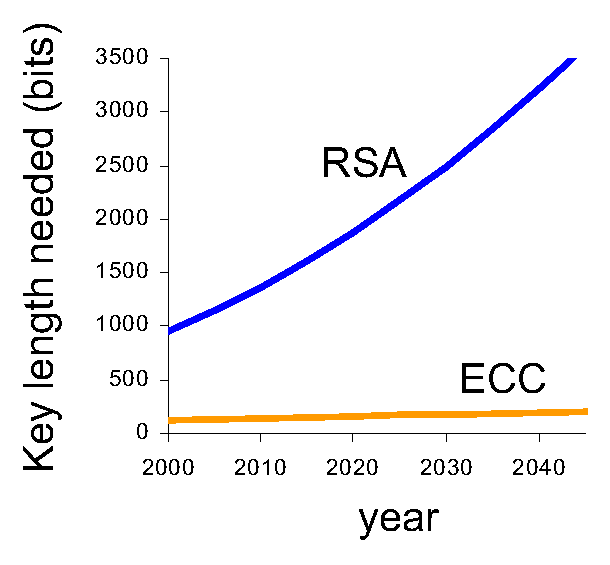
\includegraphics[scale=0.75]{figures/RSAKeylength}
\caption{Prognosis of the key lengths to be regarded safe for RSA and
  Elliptic Curves\vspace{1ex}} 
\label{RSAKeylength}
\end{center}
\end{figure}

In addition, a digital signature can be processed 10-times faster with ECC
than with RSA.  However, verification of a given signature is still more
efficient with RSA than with ECC. Refer to
figure~\ref{ThousandBitMultiplications} (source: Dr.~J.\ Merkle, Elliptic
Curve Cryptography Workshop, 2001) for a comparison.  The reason is that
RSA public keys can be chosen relatively small as long as the secret key is
sufficiently long.

% -> Figure 2
\begin{figure}[h]
\begin{center}
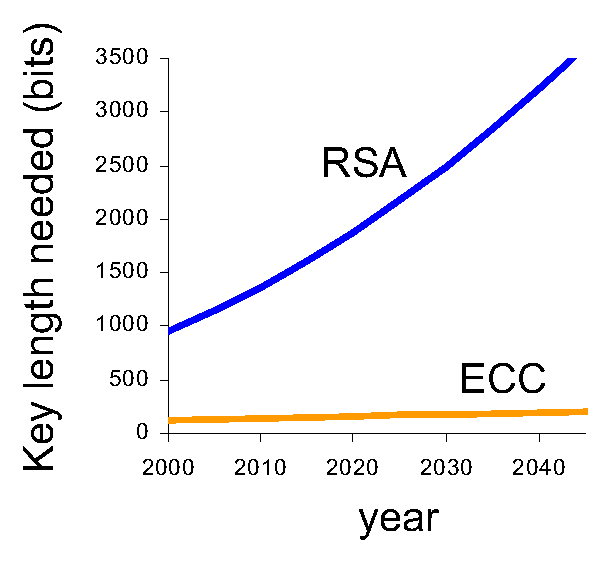
\includegraphics[scale=0.75]{figures/ThousandBitMultiplications}
\caption{Comparison of signing and verification time for RSA and Elliptic Curves} 
\label{ThousandBitMultiplications}
\end{center}
\end{figure}

Nevertheless, thin clients like smart cards usually have to store the (long) secret key
and have to process a digital signature rather than to verify one. Therefore, there is
a clear advantage for ECC in terms of efficiency.
\par
\smallskip
Today, the major problem with ECC-implementations is the lack of standardization.
There is only one way to implement RSA, but there are many ways for ECC: One can work with
different sets of numbers, different (elliptic) curves described by up to 6 parameters,
and a variety of representations of the elements on the curve. Each choice has its
advantages and disadvantages, and one can certainly construct the most efficient for
each application. However, this causes problems in interoperability. But if all
ECC-tools should be able to communicate with each other, they will have to support
all different algorithms, which might put the advantage of efficient computation and
the need of less storage capacity to the contrary.

Therefore, international standardization organizations like IEEE (P1363),
ASC (ANSI X9.62, X9.63), ISO/IEC as well as major players like RSA labs or
Certicom have recently started standardization initiatives. While the IEEE
only describes the different implementations, the ASC has explicitly stated
10 elliptic curves and recommends their usage. The advantage of the ASC
approach is that one needs only a single byte to indicate which curve is
meant. However, it is not clear yet whether the ASC-curves will become a de
facto standard.

Although we see no need to replace RSA in any application today, one should
take the usage of ECC-based tools into consideration whenever a new system
is set up --- in particular, when the tool should be available beyond 2005.


\subsection{Elliptic curves --- history}

Mathematicians have been researching elliptic curves for over 100 years. In the
course of time, many lengthy and mathematically complex results have been found
and published in connection with elliptic curves. A mathematician would say that
elliptic curves (or the mathematics behind them) are widely understood. This
research was originally purely mathematical. That is to say, elliptic curves
were investigated, for example, in the mathematical areas of number theory and
algebraic geometry, which are generally highly abstract. Even in the recent
past, elliptic curves played an important role in pure mathematics. In 1993 and
1994, Andrew Wiles\index{Wiles} published mathematical works that triggered enthusiasm far
beyond the specialist audience. In these works, he proved a conjecture put
forward in the 1960's. To put it short, this conjecture was concerned with the
connection between elliptic curves and what are called module forms. That which
is interesting for most people is that the works of Wiles also proved the famous
second theorem of Fermat. Mathematicians had spent centuries (Fermat lived from
1601 to 1665) trying to find a strict proof of this theorem. Understandably,
therefore, Wiles' proof got a good response. Fermat formulated his theorem as
follows (written in the border of a book):

\begin{quote} {\em
Cubum autem in duos cubos, aut quadratoquadratum in duos quadratoquadratos, et
generaliter nullam in infinitum ultra quadratum potestatem in duos ejusdem
nominis fas est dividere: cujus rei demonstrationem mirabilem sane detexi. Hanc
marginis exiguitas non caperet.
} \end{quote}

Translated freely, using the denotation of modern mathematics, this means: \\
No positive whole numbers $x, y$ and $z$ greater than zero exist such that $x^n +
y^n = z^n$ for $n>2$. I have found an amazing proof of this fact, but there is
too little space in the border [of the book] to write it down.

This is truly amazing: A statement that is relatively simple to understand (we
are referring to Fermat's second theorem here) could only be proved after such a
long period of time, although Fermat himself claimed to have found a proof.
What's more, the proof found by Wiles is extremely extensive (all of Wiles
publications connected with the proof made up a book in themselves). This should
therefore make it obvious that elliptic curves are generally based on highly
complex mathematics.

Enough about the role of elliptic curves in pure mathematics. In 1985 Neal
Koblitz and Victor Miller independently suggested using elliptic curves in
cryptography. Elliptic curves have thus also found a concrete practical
application. Another interesting field of application for elliptic curves is for
factorising whole numbers. (For example the RSA cryptography system is based on
the \index{Complexity} difficulty/complexity of finding prime factors of an
extremely large number.) In this area, procedures based on elliptic curves have
been investigated and partially used since 1987 (a study by H.W. Lenstra). There
are also prime number tests\index{Prime number!test} based on elliptic curves.

Elliptic curves are used differently in the various areas. Encryption procedures
based on elliptic curves are based on the difficulty of a problem known as
elliptic curve discrete logarithm\index{Logarithm problem!discrete}. The factorisation of whole numbers uses the
fact that a large number of elliptic curves can be generated for a natural
composite number $n$ with several prime factors; however, these curves are not
then groups for composite $n$. \hyperlink{faktell}{More information about this
can be found under Factorisation using elliptic curves.}

\subsection{Elliptic curves --- mathematical basics}

This section provides information about \index{Group} {\em groups} and
\index{Field} {\em fields}.

\subsubsection{Groups}

Because the term {\em group} is used differently in everyday language than in
mathematics, we will, for reasons of completeness, begin by introducing the
essential statement of the formal definition of a group:
\begin{itemize}
   \item A group is a non-empty set $G$ and an operation $+.$ The set $G$ is
closed under the operation $+.$ Regardless of which two elements $a, b$ from $G$
are taken, performing the operation on them gives an element in $G$ (i.e.
$a+b=c$, and $c$ lies in $G$).
   \item For all elements $a, b$ and $c$ in $G$: $(a+b)+c = a+(b+c)$.
   \item There exists an element $e$ in $G$ that behaves neutrally with respect
to the operation $+$. That means that for all a in the set $G: ~a+e = e+a = a.$
   \item For each element $a$ in $G$ there exists a so-called inverse element $-a$
($-a$ also lies in $G$) such that: $a+(-a) = (-a)+a = e$.
\end{itemize}
If also $a+b = b+a$ for all $a, b$ in $G$ then we call the group an {\em
Abelian} group. An operation denoted as $+$ indicates an {\em additive} group;
if the operation is denoted as $\cdot$, we speak of a {\em multiplicative}
group.

The simplest example of an (Abelian) group is the group of whole numbers under
the standard operation of addition. The set of whole numbers is denoted as
${\mathbb Z}$. ${\mathbb Z}$ has an infinite number of elements, because
${\mathbb Z} = \{ \cdots, -4, -3, -2, -1, 0, 1, 2, 3, 4, \cdots\}$. For example, the
operation of $1+2$ lies in ${\mathbb Z}$, for $1+2 = 3$ and $3$ lies in
${\mathbb Z}$. The neutral element in the group ${\mathbb Z}$ is $0$. The
inverse element of $3$ is $-3$, for $3+(-3) = 0$.

There are also {\em finite} groups. This means that these exists a set
$\mathcal{M}$ with a fixed number of elements and an operation $+$ such that the
above conditions are fulfilled. One example of this is any set ${\mathbb Z}_n$
where ${\mathbb Z}_n = \{0, 1, 2, 3, \cdots, n-1\}, n$ is a positive whole number
and the operation is addition mod $n$, i.e. $a$ and $b$ in ${\mathbb Z}_n$ are
subject to the operation $a+b \;{\rm mod~} n$.

\paragraph{Cyclic groups}
Cyclic groups\index{Group!cyclic} are those groups $G'$ that possess an element $g$
from which the group operation can be used to generate all other
elements in the group. This means that for each element $a$ in
$G'$ there exists a positive whole number $i$ such that if $g$ is
subject to the operation $i$ times (i.e. ``$g \cdot i$''),
$g+g+\cdots+g = a$ (additive group) or $g^i = g\cdot g \cdots g = a$
(multiplicative group). The element $g$ is the {\em generator} of
the cyclic group --- each element in $G�$ can be generated using
$g$ and the operation.

Now to the order of an element of the group: Let $a$ be in $G$. The smallest
positive whole number $r$ for which $a$ subject to the operation with itself $r$
times is the neutral element of the group $G�$ (i.e.: $r \cdot a = a+a+\cdots+a =
e$ bzw.\ $a^r = e$), is called the {\em order} of $a$.

The order of the group is the number of elements in the set $G$.

\subsubsection{Fields}

In mathematics, a field is understood to be a set $K$ with two operations
(denoted as $+$ and $\cdot$) which fulfils the following conditions:
\begin{itemize}
   \item The set $K$ forms an Abelian group together with the operation $+$
(addition), where $0$ is the neutral element of the operation $s$.
   \item The set $K$ (without the element 0) also forms an Abelian group
together with the operation $\cdot$ (multiplication).
   \item For all elements $a, b$ and $n$ in $K$, $n\cdot (a+b) = n \cdot a + n
\cdot b$ and $(a+b) \cdot n = a \cdot n + b \cdot n$.
\end{itemize}

There are {\em infinite} fields, i.e. the set on which the field is based
contains an infinite number of elements (e.g.: the field of real numbers). And
there are also finite fields, such as ${\mathbb Z}_p = \{0, 1, 2, 3, \cdots, p-1\}$
, where $p$ is a prime. ${\mathbb Z}_p$ with addition mod $p$ and multiplication
mod $p$ is a finite field.
\index{Field!Characteristic}
\paragraph{Characteristic of a field}
Let $K$ be a field and $1$ be the neutral element of $K$ with
respect to the multiplicative operation ``$\cdot$''. For positive
natural numbers $n$, let us understand $n_1$ to be $n_1 = 1 + 1 +
\cdots + 1$ ($n$ summands and $n_1$ is an element in $K$). If $n_1$
is then unequal to $0$ for all $n>0$, then we call $K$ a field
with characteristic zero. Otherwise, the characteristic of $K$ is
defined to be the smallest positive natural number $p$ for which
$p_1 = 0$ (note: $p$ is then a prime). Comment: The field of real
numbers has the characteristic $0$; the field ${\mathbb Z}_p$ has
the characteristic $p$.

\subsection{Elliptic curves in cryptography}

An elliptic curve is described by an equation. In order to keep it simple, we
restrict our explanation to elliptic curves over $${\mathbb Z}_p = \{0, 1, 2, 3,
\cdots, p-1\}$$ where $p$ is a prime greater than $3$. ${\mathbb Z}_p$ with
addition mod $p$ and multiplication mod $p$ is a finite field. However, we must
mention that elliptic curves can be defined over any (finite) field. In
particular, elliptic curves over fields with characteristic $2$ are extremely
interesting from a practical point of view because computers can be used to
represent the elements from these fields as bit strings. This leads to an
efficient implementation of the arithmetic in such fields, which means that a
computer can perform the operations of the field particularly quickly.

Because these points actually refer to the same thing, it is seldom necessary to distinguish between exact meanings.

An elliptic curve over ${\mathbb Z}_p$ is defined by an equation of the following form:
$$ y^2 \; ({\rm mod} \; p) = x^3 + ax + b ({\rm mod} \; p) $$
(thus: equality in the field ${\mathbb Z}_p$), where $a, b$ are in ${\mathbb Z}_p$ and $4a^3 + 27b^2$ mod $p$ is
not equal to zero. For fixed chosen numbers $a$ and $b$ in ${\mathbb Z}_p$, this equation has the pair of solutions
$$ {\bf E} = \left\{(x,y) \left| \begin{array}{c} x {\rm ~and~} y {\rm ~are~in~} {\mathbb Z}_p {\rm ~and~} \\
y^2  \equiv x^3 + ax + b \;({\rm mod~} p) {\rm ~and~} \\ 4a^3 + 27b^2 \not\equiv 0 \;
({\rm mod~} p)\end{array} \right. \right\}, $$ i.e. the set ${\bf E}$ consists of all pairs $x$ and $y$ that are a solution
(in ${\mathbb Z}_p$) of the above equation. It must be noted that the numbers $a, b$ and $p$ determine which pairs $(x,y)$
lie in the set ${\bf E}$. This means that $a, b$ and $p$ specify this set. The elements $(x,y)$ in ${\bf E}$ are called
points on the elliptic curve. In addition, ${\bf E}$ has one more element $O$ (the so-called point in infinity).
The set ${\bf E}$ is usually called an elliptic curve. 

We can now define an operation\footnote{A animated addition of elliptic curve points can be
found at the web page of Certicom\index{Certicom}:
\href{http://www.certicom.com/resources/ecc_tutorial/ecc_tutorial.html}{\tt http://www.certicom.com/resources/ecc\_tutorial/ecc\_tutorial.html}.}
(also denoted as $+$, although it is
not the standard/usual addition of real numbers) on two elements in ${\bf E}$ such that the operation delivers an element
that also lies in ${\bf E}$. The set ${\bf E}$ is therefore closed under the operation $+$. We can show
that ${\bf E}$ is a group. The neutral element of the group ${\bf E}$ is the point in infinity $O$. Thus, for every two
points $(x_1,y_1)$ and $(x_2,y_2)$ on the elliptic curve ${\bf E}$, there exists a point $(x_3,y_3)$ on ${\bf E}$ such that
the operation $+$ complies with the following: $(x_1,y_1) + (x_2,y_2) = (x_3,y_3)$. Under certain circumstances, these points
may also be equal to the point in infinity. Thus, when we speak of a point $P$ on an elliptic curve ${\bf E}$,
we mean that $P = (x,y)$ and $(x,y)$ lies in the set ${\bf E}$. Any two points on an elliptic curve specified by $a, b$ and $p$
can therefore be added and the result is a point that also lies on the same elliptic curve.

% \newpage
\begin{figure}[htbp]
\subsubsection*{Adding of two points on an elliptic curve}
The following two figures show an elliptic curve in the affine plane and
shows how points on an elliptic curve are added. Note that the point in infinity $O$ cannot be represented in
the affine plane.
\begin{center}
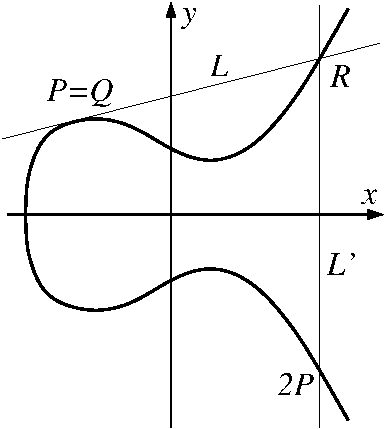
\includegraphics[scale=1.08]{figures/ec-mult2}
\caption{Doubling the point P} \vspace{\floatsep} \vskip +20 pt
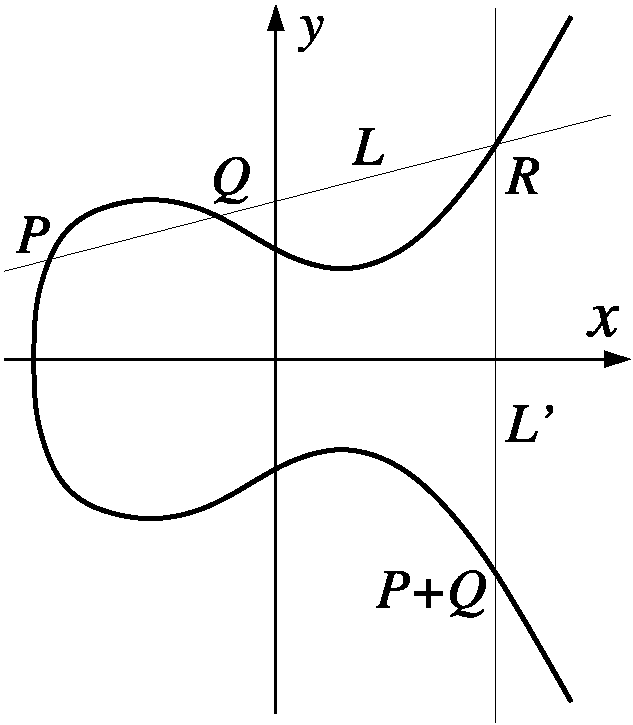
\includegraphics[scale=0.65]{figures/ec-add}
\caption{ Adding distinct points P and Q} % \footnotemark}
\end{center}
\end{figure}
% \addtocounter{footnote}{0}\footnotetext{The point $O$ cannot be represented in the affine plane.}
\enlargethispage{+20pt}

\newpage
We must note that ${\bf E}$ can have the following meanings:
\begin{itemize}
   \item the set ${\bf E}$ of solutions pairs $(x,y)$ for an equation including the point $O$
   \item the group ${\bf E}$ (with the operation ``addition of $(x_1,y_1)$ and $(x_2,y_2)$'')
   \item the elliptic curve ${\bf E}$ (which is actually the same as the group ${\bf E}$)
\end{itemize}
For cryptography, the important fact is that, for very large numbers, it appears to be extremely difficult to use a
given point $Q$ on an elliptic curve to determine which two points have to be added to obtain $Q$.

For large numbers $a, b$ and $p$ ($p$, for example, has a length of more than $160$ bits), the computer can easily add
the point $P$  $m$ times after another, i.e. to determine the point $P + P + \cdots + P = Q$ in an incredibly short space
of time (in a few fractions of a second) ($m$ summands $P$). Rather than $P + P + \cdots + P = Q$ ($m$ summands $P$)
we also write $mP = Q$. If we have a point $P$ and a point $Q$, which both lie on the same elliptic curve, no procedure
is known that enables us --- within an acceptable space of time --- to determine the number $m$ (assuming it actually exists)
for which $mP = Q$. This is referred to as the ``elliptic curve discrete logarithm problem'' (abbreviated to ECDLP)\index{ECDLP}.

We must note that not all elliptic curves are equally secure. This
means that we must choose the parameters $a$ and $b$ carefully
when defining a curve. For certain classes of elliptic curves, it
is possible to solve the ECDLP easier than in the general case.
Cryptographically unsuitable elliptic curves are called {\em abnormal}
curves (these are curves over ${\mathbb Z}_p$ for which the set
${\bf E}$ has precisely $p$ elements) and the {\em supersingular} curves
(the curves for which we can reduce the calculation of the ECDLP
to calculating the ``standard'' discrete logarithm in other finite
fields, i.e. simplify the calculation). There are therefore
cryptographically good and bad curves. However, for given
parameters $a$ and $b$ we can, with some difficulty, establish
whether or not the resulting elliptic curve is useful for
cryptographic purposes. The curves used in cryptography are
usually provided by experts. They ensure that the elliptic curves
they classify as secure satisfy the current security requirements.

For secure curves, the parameter $p$ determines how long it takes
to solve the ECDLP on this curve. The larger the parameter $p$,
the longer it takes to solve the problem. Experts recommend a bit
length of over $200$ bits for the parameter $p$. This makes it
clear why elliptic curves are so interesting for cryptography.
Because the parameter $p$ also determines the time required to
perform the signature/encryption procedure when using elliptic
curves in cryptography. The time taken to generate a pair of keys
also depends on $p$. Thus, small values (few bits) are desirable
here (in order to minimise the run times for the procedures);
however, the required security must still be maintained. For
example, with a length of $200$ bits for $p$, a {\em good}
elliptic curve is just as secure as an \index{RSA!module} RSA
module of over $1024$ bits in length (at least according to the
current state of research). The reason for this is that the
quickest algorithms for solving the {\em elliptic curve discrete
logarithm} problem have an exponential run time --- unlike the
sub-exponential run times that the best factorisation algorithms
currently have (number sieve, quadratic sieve or factorisation
with elliptic curves). Therefore, the parameters for cryptographic
procedures based on the problem of {\em factorising whole numbers}
must be greater than the parameters for cryptographic procedures
based on the ECDLP problem.

\subsubsection{Digital signatures using elliptic curves}

The {\em elliptic curve discrete logarithm problem} (ECDLP) \index{ECDLP} forms the basis for
elliptic-curve cryptography. Various signature procedures are based on this.
What they have in common is how they use the public parameters and how these
parameters are used to generate secret and public keys:
\begin{itemize}
    \item The parameters of the elliptic curve E, i.e. a prime number $p$ that
determines over which field ${\mathbb Z}_p$ the elliptic curve ${\bf E}$ is
defined, as well as the two numbers $a$ and $b$ in ${\mathbb Z}_p$.
    \item A point $G=(x,y)$ that lies on the elliptic curve ${\bf E}$.
    \item A prime number $r < p$ for which $rG=O$ (i.e. $G$ added $r$ times
gives the neutral element of the group ${\bf E}$) and $r$ is a factor of $\#{\bf
E}$ (where $\# {\bf E}$ is the number of elements in the set ${\bf E}$). The
point $G$ therefore has the order $r$ and is the generator of a cyclic subgroup
of ${\bf E}$ with the order $r$.
    \item The number $k = \#{\bf E}/r$ ($k$ is called the {\em cofactor}).
\end{itemize}
The parameters $a, b, p, G, r$ and $k$ listed above are called
{\em domain parameters}.\index{Domain parameters} They determine on which elliptic curve ${\bf
E}$ and in which cyclic subgroup of ${\bf E}$ a signature
procedure has been ``used''.

The secret key $s$ of the signature generator is a (random) whole number $s$ in
the interval $[1, r-1]$. The public key of the signature generator is a point
$W=(x,y)$ on the elliptic curve ${\bf E}$. The public key $W$ and secret key $s$
are interrelated as follows: $W = sG$. This means that the domain parameters
(particularly $G$) and the secret key $s$ are used to calculate the public key
$W$ (by adding $G$ $s$ times on ${\bf E}$). The ECDLP is obviously used here: If
$W$ and $G$ (as well as the other domain parameters used) are known, then it is
difficult to use these to calculate $s$. (If the parameters are chosen
correctly, this currently appears to be practically impossible).

In order to verify a signature, the recipient of the signature must know the
following:
\begin{enumerate}
   \item The signature procedure used,
   \item The hash function used,
   \item The domain parameters used to generate the signature
   \item The public key $W$ of the signature generator.
\end{enumerate}


\subsubsection{Factorisation using elliptic curves}

\hypertarget{faktell}{}

There are factorisation algorithms based on elliptic curves
\footnote{In 1987 H.W. Lenstra published
a factorisation algorithm, based on elliptic curves (see \cite{Lenstra1987}).
The biggest compound number currently factorised with elliptic curves is 
the number $ 628^{59}-1, $ which has 55 decimal digits. It was
found Oct. 6th, 2001 by M. Izumi 
(See \hyperlink{Lenstra2}{ECMNET}\index{ECMNET}).
}. 
More precisely, these procedures exploit the fact that elliptic curves can
be defined over ${\mathbb Z}_n$ ($n$ composite number). Elliptic curves 
over ${\mathbb Z}_n$ do not form a group, because not every point on such 
an elliptic curve has an inverse point. This is connected with the fact 
that - if $n$ is a composite
number - there exist elements in ${\mathbb Z}_n$ that do not have an inverse
with respect to multiplication mod $n$. In order to add two points on an
elliptic curve over ${\mathbb Z}_n$, we can calculate in the same way as on
elliptic curves over ${\mathbb Z}_p$. Addition of two points (on an elliptic
curve over ${\mathbb Z}_n$), however, fails if and only if a factor of $n$ has
been found. The reason for this is that the procedure for adding points on
elliptic curves gives elements in ${\mathbb Z}_n$ and calculates the inverse
elements for these (with respect to multiplication mod $n$) in ${\mathbb Z}_n$.
The extended \index{Euclidean algorithm} Euclidean algorithm is used here. If
the addition of two points (that lie of an elliptic curve over ${\mathbb Z}_n$)
gives an element in ${\mathbb Z}_n$ that does not have an inverse element in
${\mathbb Z}_n$, then the extended Euclidean algorithm delivers a genuine factor
of $n$.

Factorisation using elliptic curves thus principally works as follows: You
select random curves over ${\mathbb Z}_n$, as well as random points (that lie on
this curve) and add them; you thus obtain points that also lie on the curve or
find a factor of $n$. Factorisation algorithms based on elliptic curves
therefore work probabilistically. The opportunity of defining large number of
elliptic curves over ${\mathbb Z}_n$ allows you to increase the probability of
finding two points which you can add to obtain a factor of $n$. These procedures
are therefore highly suitable for parallelisation.

\subsection{Implementing elliptic curves}

CrypTool\index{CrypTool} uses elliptic curves for the digital signature function.

It implements the basic algorithms for group operations, for generating elliptic
curves, for importing and exporting parameters for elliptic curves over finite
fields with $p$ ($p$ prime) elements. The algorithms have been implemented in
ANSI C and comply with draft no. 8 of the IEEE P1363 work group {\em Standard
Specifications for Public Key Cryptography}

{\href{http://grouper.ieee.org/groups/1363}{\tt
http://grouper.ieee.org/groups/1363}}.

The procedure implements the cryptographic primitives for generating and
verifying signatures for the variations of Nyberg-Rueppel signatures and
\index{DSA} DAS signatures based on elliptic curves (in accordance with draft
no. 8 of the IEEE P1363 work group). This was done in collaboration with the
Secude GmbH --- using the above library and the Secude SDK.
\index{Secude}

\newpage
%\addcontentsline{toc}{subsection}{Literaturverzeichnis}
\begin{thebibliography}{99999}
\addcontentsline{toc}{subsection}{Bibliography}
        \bibitem[Lenstra1987]{Lenstra1987} H.W. Lenstra\\ \index{Lenstra 1987}
                Factoring integers with elliptic curves, Annals of Mathematics 126, pp. 649-673, 1987.
\end{thebibliography}
%\newpage

\section*{Web links}\addcontentsline{toc}{subsection}{Web links}

\begin{enumerate}
   \item Certicom Online Tutorial, \index{Certicom}\\
                \href{http://www.certicom.com/resources/ecc_tutorial/ecc_tutorial.html}{\texttt{http://www.certicom.com/resources/ecc\_tutorial/ecc\_tutorial.html}}
        \item IEEE P1363

                \href{http://grouper.ieee.org/groups/1363}{\texttt{http://grouper.ieee.org/groups/1363}}
        \item  \hypertarget{Lenstra2}{}
An informative web page about factorisation with elliptic curves.

\href{http://www.loria.fr/~zimmerma/records/ecmnet.html}{\texttt{http://www.loria.fr/\~{}zimmerma/records/ecmnet.html}}

There, one finds literature to the topic factorisation with elliptic curves as well as links to other web page. 

\end{enumerate}


% Local Variables:
% TeX-master: "../script-en.tex"
% End:

\bibliographyunit[\chapter]
\bibliography*{../de/references}
\bibliographystyle*{plain}
% ..........................................................................
% --------------------------------------------------------------------------
% ++++++++++++++++++++++++++++++++++++++++++++++++++++++++++++++++++++++++++
%              Crypto 2020
% /~~~~~~~~~~~~~~~~~~~~~~~~~~~~~~~~~~~~~~~~~~~~~~~~~~~~~~~~~~~~~~~~~~~~~~~~~

\newpage
\hypertarget{Chapter_Crypto2020}{}
\chapter{Crypto2020 --- Perspectives for long-term cryptographic
         security\index{Security!long-term}}
\label{Chapter_Crypto2020}
\begin{sloppypar}
(Johannes Buchmann, Erik Dahmen, Alexander May and Ulrich Vollmer, TU Darmstadt, May~2007)\\
\end{sloppypar}

% \begin{abstract}Ever more powerful hardware and new
%   mathematical algorithms threaten to undermine
%   the security of cryptographic keys and schemes.
%   How long will the methods we use today be able
%   to keep what they promise?  And which
%   alternatives are on the horizon?
% \end{abstract}

Cryptography is a basic building block of all IT
security solutions.  Yet, for how long are the
cryptographic tools we use today going to remain
secure?  Is this time long enough to ensure the
confidentiality of medical data, to name just one
example?  Even in the short-term, the potential
for havoc is great if certain keys are broken.
Just think of the digital signatures that protect
the authenticity of automatic updates for the
Windows operating system.


\section{Widely used schemes}
\label{sec:the-weak}

In 1978, Rivest, Shamir and Adleman suggested the
RSA\index{RSA} public key encryption and signature
schemes~\cite{rivest/shamir/adleman:1978}.  RSA is
still the most widely used public key scheme.  The
security of RSA depends on the difficulty of
factoring so-called RSA moduli which are products
of two large prime numbers.  In their 1978 paper,
the inventors of RSA suggested the use of RSA
moduli with 200 decimal digits for long-term
security.  Later, the company RSA Security
published a list of RSA moduli of increasing size,
the RSA challenge numbers.  RSA Security offered
prizes totaling \$ 635,000 for the factorization
of these numbers, cf.\
\url{www.rsasecurity.com/rsalabs/}.

In 2005, that is 27 years after the invention of
RSA, Bahr, Boehm, Franke, and Kleinjung from
Bochum University managed to factor a 200 digit
RSA challenge number
(\url{www.mat.uniroma2.it/~eal/rsa640.txt}).  A
key with size originally thought to be secure for
a very long time was broken with a computation
that took them just five months.  This illustrates
the tremendous progress factoring technology has
made within the last 30 years.  This progress is
based on break-through mathematical ideas --- e.g.\
the number field sieve proposed by John
Pollard --- as well as significant developments in
computer hardware and software implementation
technology.\footnote{%
Please compare chapter \ref{SecurityRSA}
\hyperlink{SecurityRSA}{Considerations regarding the
security of the RSA algorithm}, and especially chapters
\ref{NoteFactorisation} and \ref{FactorisationResearch}.
}

In 2000, Lenstra and Verheul\index{Lenstra/Verheul}
developed an extrapolation formula that is supposed
to help us forecast the security\index{Security!forecast}
one can achieve with RSA and other important
cryptographic schemes in the long
term (\url{www.keylength.com}).  The formula
suggests the use of 850 digit RSA moduli if one
wishes to protect data for the next 30 years.
This corresponds to a 3072 bit RSA key.

Yet, even a well thought out extrapolation formula
is no security guarantee!  At any time, a
brilliant mathematical idea can allow us to factor
large numbers easily, and destroy the security of
RSA.  In 1996, Peter Shor showed that a quantum
computer --- a new type of computer that leverages
the laws of quantum mechanics to speed up certain
types of computations --- can in principle be used
for the fast factorization of large numbers \cite{shor:1997}.
Despite intensive research in the area, it is
still too early to judge whether we are ever going
to be able to build quantum computers\index{Quantum computer} of
sufficient capacity to apply Shor's algorithm to
numbers of relevant size.\footnote{%
Required qbits for attacks on RSA, DSA and ECDSA using key with a bit length n: \\
\vskip +1 pt
\begin{tabular}{|c|l|}
\hline
   RSA		&  2n + 3 \\
   DSA		&  2n + 3 \\
   ECDSA $2^n$	&  \~{}2n + 8 log n \\
   ECDSA p	&  \~{}4n \\
\hline
\end{tabular}
\vskip +6 pt
Please compare chapter 5.3 in
``SicAri -- Eine Sicherheitsplattform und deren Werkzeuge
f\"ur die ubiquit\"are Internetnutzung, KB2.1 -- Abschlussbericht,
\"Ubersicht \"uber Angriffe auf relevante kryptographische Verfahren'',
version 1.0, Mai 17, 2005,
Prof. Dr. Johannes Buchmann et al., TUD-KryptC and cv cryptovision GmbH
(\href{http://www.cdc.informatik.tu-darmstadt.de/~schepers/kb\_21\_angriffe.pdf}
 {\tt http://www.cdc.informatik.tu-darmstadt.de/\~{}schepers/kb\_21\_angriffe.pdf}) and the dissertation of Axel Schmidt at the same faculty.
}
Recent announcements of
significant progress in this area made by the
start-up company D-Wave (\url{www.dwavesys.com})
have been greeted with a lot of scepticism, even
ridicule.

The development of attacks on another frequently
used scheme called DSA (Digital Signature
Algorithm) and the Elliptic Curve Cryptography
(ECC) class of schemes moves in analogy to those
on RSA.  The security of these schemes depends on
the difficulty of computing discrete logarithms.
Even today, there is significant algorithmic
progress.  Quantum computers would render these
schemes insecure.

What's the state of affairs with the so-called
secret-key encryption schemes?  In 1977, DES was
introduced as the Data Encryption
Standard~\cite{DES-Standard:1977}.  Twenty-one
years later, the Electronic Frontier Foundation
(EFF) built the special purpose machine Deep Crack
which needed just 56 hours to break a DES key.
The problem with DES was that it used keys which
were too short.  It seems that the inventors of
DES did not foresee the speed of hardware
development.  The Advanced Encryption Standard
AES~\cite{AES-Standard:2002}, successor to DES, is
deemed secure at the moment even though there are
interesting, if still inefficient, methods to
attack AES with algebraic methods.


\section{Preparation for tomorrow}
\label{sec:preparations}

Is the security of today's cryptography measuring
up to its increasing importance?  The experience
shows: Carefully designed and implemented
cryptographic schemes have a life time of five to
twenty years.  Whoever uses RSA, ECC or AES for
short-term protection of data may feel safe.
Moreover, it is also possible to achieve long-term
authenticity, integrity and non-reputability of
data, e.g., using the multiple signature scheme
suggested by S\"onke Maseberg~\cite{maseberg-thesis:2002}.

However, current schemes cannot guarantee
long-term confidentiality.  And what is to be done in
twenty years from now?  What should we do if, quasi
over-night, unexpected mathematical progress
renders an important cryptographic scheme
insecure?  Three things are necessary to prepare
us for this event:

\begin{itemize}
\item a pool of secure alternative cryptographic schemes,
\item infrastructures that enable us to exchange
   one cryptographic scheme for another, easily
   and quickly, and
\item methods that ensure long-term confidentiality.
\end{itemize}

For many years, the cryptography group at the
Technische Universit\"at Darmstadt and its spin-off,
the company FlexSecure (\url{www.flexsecure.de}),
have worked to provide these tools.  The
trust center software FlexiTrust which is employed
by the German National Root Certification
Authority and the German Country Signing Authority
offers an infrastructure within which
cryptographic schemes can be easily exchanged.
The open source library FlexiProvider\index{FlexiProvider} implements a
multitude of cryptographic schemes.  Lately, we
have intensified our research into ``Post Quantum
Cryptography''\index{Cryptography!Post Quantum} seeking
cryptographic schemes which
remain secure even in the event that powerful
quantum computers are built.

The security of public key cryptography
traditionally rests on the difficulty of the
solution of certain mathematical problems.  Today,
the following alternatives to the factorization and discrete
logarithm problems are discussed in depth:  the
decoding problem, the shortest and closest vector
problem in lattices, and the problem of solving
large systems of multivariate quadratic
equations.  It is conjectured that quantum
computers\index{Quantum computer} offer little advantage if we try to
solve these problems efficiently.


\section{New mathematical problems}
\label{sec:problems}

Let us look at these alternatives a little more
closely.  The first encryption scheme based on the
decoding problem was proposed by
McEliece~\cite{mceliece:1978}\index{Encryption!McEliece}.  The background:
Error-correcting codes are used to transmit or
store electronic data in such a way that they
remain undistorted even if a small number of bits
are changed in transit or on the storage media.
This property is used in, e.g., compact discs
(CDs).  The data on a CD can be reconstructed even
if the disc has been slightly scratched.

In a code-based encryption\index{Encryption!code-based} scheme a message is
encrypted by adding a fixed number of errors to
(i.e. flipping a fixed numbers of bits of) the
encoded message.  Decoding requires knowledge of a
suitable decoding procedure which eliminates these
errors efficiently.  This method is the secret
key.  Code-based encryption is in general very
efficient.  At the moment, research focus on the
question which codes lead to secure encryption
schemes with keys which are as small as possible.

Encryption on the basis of lattice problems\index{Encryption!lattice problems}
is very similar to that on the basis of
error-correcting codes.  Lattices are regular
structures of points in space.  For instance, the
points where the lines on squared paper cross form
a two-dimensional lattice.  For cryptographic
usage, the dimension of the lattices is chosen to
be much larger.  Encryption works as follows: The
plain-text is used to construct a lattice point
which is then slightly distorted in such a way
that it is no longer a lattice point, but close to
one.  Whoever knows a secret about the lattice is
able to find this lattice point in the vicinity of
the given point in space.  The lattice point in
turn yields the plain text.  A particularly
efficient lattice based encryption scheme is NTRU
Encrypt (\url{www.ntru.com})\index{Encryption!lattice problems!NTR}.
However, because
NTRU was introduced fairly recently (in 1998), and
its specification underwent several changes due to
a variety of attacks, more cryptanalytic scrutiny
is required to achieve confidence in its security.

\section{New signatures}
\label{sec:signatures}

In 1979, Ralph Merkle proposed a remarkable
framework for new signature schemes in his PhD
thesis~\cite{merkle-thesis:1979}.
Contrary to all other signature schemes\index{Signature!Merkle}, its
security does not rest on the difficulty of a
number-theoretic, algebraic or geometric problem.
The only thing it requires is something which
other signature schemes need anyway: a
cryptographically secure hash function and a
secure pseudo-random number generator.  Each new
hash function leads to a new signature algorithm.
In consequence, the Merkle scheme has the
potential to solve the problem of long-term
availability of digital signature schemes.

Merkle uses in his construction so-called One-Time
Signatures: Each new signature requires a new
signing key and a new verification key.  The idea
Merkle had was to reduce the validity of many
verification keys using a hash tree to the
validity of a unique public hash value.  When
generating keys for the Merkle scheme one has to
determine the number of signatures one can make
with it in advance.  For a long time this seemed a
significant disadvantage.  In
\cite{buchmann/coronado/dahmen/doering/klintsevich:2006},
however, a variant of Merkle's scheme was proposed
which allows to compute $2^{40}$ signatures with a
single key pair.


%\subsection{Quantum cryptography -- a loophole?}
\section{Quantum cryptography -- a way out of the impasse?}
\label{sec:quantum cryptography}\index{Quantum cryptography}

From the point of view of today's state of the art
of cryptography, the problem of long-term
confidentiality remains unsolved: There is
\emph{no} practical method to protect the
confidentiality of an encrypted message over a
very long period of time.

One way out of that dilemma may be to employ
quantum cryptography: it allows for key agreement
schemes (of very long keys for one-time pads)
whose security is
guaranteed by the laws of quantum mechanics,
cf., e.g., \cite{bennett/brassard:1984b}.  At the
moment, however, quantum cryptography is still
rather inefficient, and it is unclear which
cryptographic functionalities can be implemented
on top of it.


\section{Conclusion}
\label{sec:conclusion}

What's on the balance sheet of today's crypto?  We
have good tools to ensure short and medium term
security.  Software developers can employ these
tools in their applications with good conscience
as long as they make sure that components
can quickly be exchanged when they become
insecure.

In order to guarantee IT security for the future, too,
we need to prepare a portfolio of secure cryptographic
schemes.  This portfolio needs to contain schemes
which are suitable for the world of ubiquitous
computing with many less powerful computers.  It
also needs to contain schemes which remain secure
in the event that powerful quantum computers\index{Quantum computer} are
built.  Several promising candidates have been
discussed in this article.  They need to be
studied carefully and prepared for use in everyday
scenarios.  The question how to ensure long-term
confidentiality remains an important open research
problem upon which cryptographic research should
focus.

\putbib


\bibliographyunit


% ++++++++++++++++++++++++++++++++++++++++++++++++++++++++++++++++++++++++++
\begin{appendix}
\newpage
\hypertarget{appendix-start}{}\label{s:appendix-start}
\chapter{Appendix}
    \begin{itemize}
      \item[1] \hyperlink{appendix-menutree}{CrypTool Menu Tree}
      \item[2] \hyperlink{appendix-authors}{Authors of the CrypTool Script}
      \item[3] \hyperlink{appendix-authors}{Bibliography of Movies and
                     Fictional Literature with Relation to Cryptography,
                     Books for Kids with Collections of Simple Ciphers}
      \item[4] \hyperlink{appendix-Learn-NT}
                     {Learning Tool for Elementary Number Theory}
      \item[5] \hyperlink{appendix-using-sage}
                     {Using Sage with this Script}
    \end{itemize}
  \newpage
  % $Id%

% ++++++++++++++++++++++++++++++++++++++++++++++++++++++++++++++++++++++++++
\newpage
%\enlargethispage{1cm}
\hypertarget{appendix-menu-overview-CT1}{}
\section{CrypTool-1-Men�baum}
\label{s:appendix-menu-overview-CT1}

   % Eyecatcher_Neue-CrypTool-Version
Dieser Anhang enth�lt auf der folgenden Seite den kompletten Men�baum der
CrypTool\index{CrypTool}-Version 1.4.31\footnote{%
  W�hrend sich seit 2010 �nderungen an der langj�hrig stabilen Version
  CrypTool 1 ({\bf CT1})\index{CrypTool 1} vor allem auf Bugfixes beschr�nkten,
  flie�en viele Neuerungen in die beiden Nachfolgeversionen CrypTool 2
  ({\bf CT2})\index{CrypTool 2} und JCrypTool ({\bf JCT})\index{JCrypTool}
  ein:\\
  - Webseite CT2: \url{http://www.cryptool.org/de/ct2-documentation-de} \\
  - Webseite JCT: \url{http://www.cryptool.org/de/jct-machmit-de} \\
  Diese Nachfolgeversionen sind zur Zeit (Nov. 2012) noch Betaversionen;
  sie stehen aber kurz vor ihrem jeweiligen ersten Release und sind schon
  l�nger stabil genug, um von Endbenutzern genutzt werden zu k�nnen.
}.

\noindent Das Haupt-Men� von CT1 enth�lt die generellen Service-Funktionen
in den sechs Haupt-Men�-Eintr�gen
\begin{itemize}
   \item Datei
   \item Bearbeiten
   \item Ansicht
   \item Optionen
   \item Fenster
   \item Hilfe,
\end{itemize}
und die eigentlichen Krypto-Funktionen in den vier Haupt-Men�-Eintr�gen
\begin{itemize}
   \item Ver-/Entschl�sseln
   \item Digitale Signaturen/PKI
   \item Einzelverfahren
   \item Analyse.
\end{itemize}

Unter \verb#Einzelverfahren# finden sich auch die Visualisierungen von Einzelalgorithmen und von Protokollen. Manche Verfahren sind sowohl als schnelle Durchf�hrung (meist unter dem Men� \verb#Ver-/Entschl�sseln#) als auch als
Schritt-f�r-Schritt-Visualisierung implementiert.

Welche Men�eintr�ge in CrypTool 1 gerade aktiv (also nicht ausgegraut) sind,
wird durch den Typ des aktiven Dokumentfensters bestimmt:
So ist z.~B. die Brute-Force-Analyse\index{Angriff!Brute-Force} f�r DES 
nur verf�gbar, wenn das aktive Fenster in Hexadezi"-mal-Darstellung 
ge�ffnet ist, w�hrend der Men�eintrag "`Zufallsdaten erzeugen\dots"'
immer verf�gbar ist (auch wenn kein Dokument ge�ffnet ist). 

%Folgende vier Dokumenttypen gibt es in CrypTool:
%\begin{center}
%\begin{tabular}{rl}
%\bf Codebuchstabe & \bf Dokumententyp \\
%T & Textdatei-Ansicht\\
%H & Hexadezimal-Ansicht\\
%P & Diagramm/Plot-Ansicht (Histogramm, Autokorrelation)\\
%O & OpenGL Graphics-Ansicht\\
%\end{tabular}
%\end{center}


%--------------------------------------------------------------------
\clearpage
\begin{figure}[hb]
\begin{center}
\vspace{-30pt}
%\frame{
%\includegraphics[scale=0.25, angle=270, viewport=200 30 2680 1420]
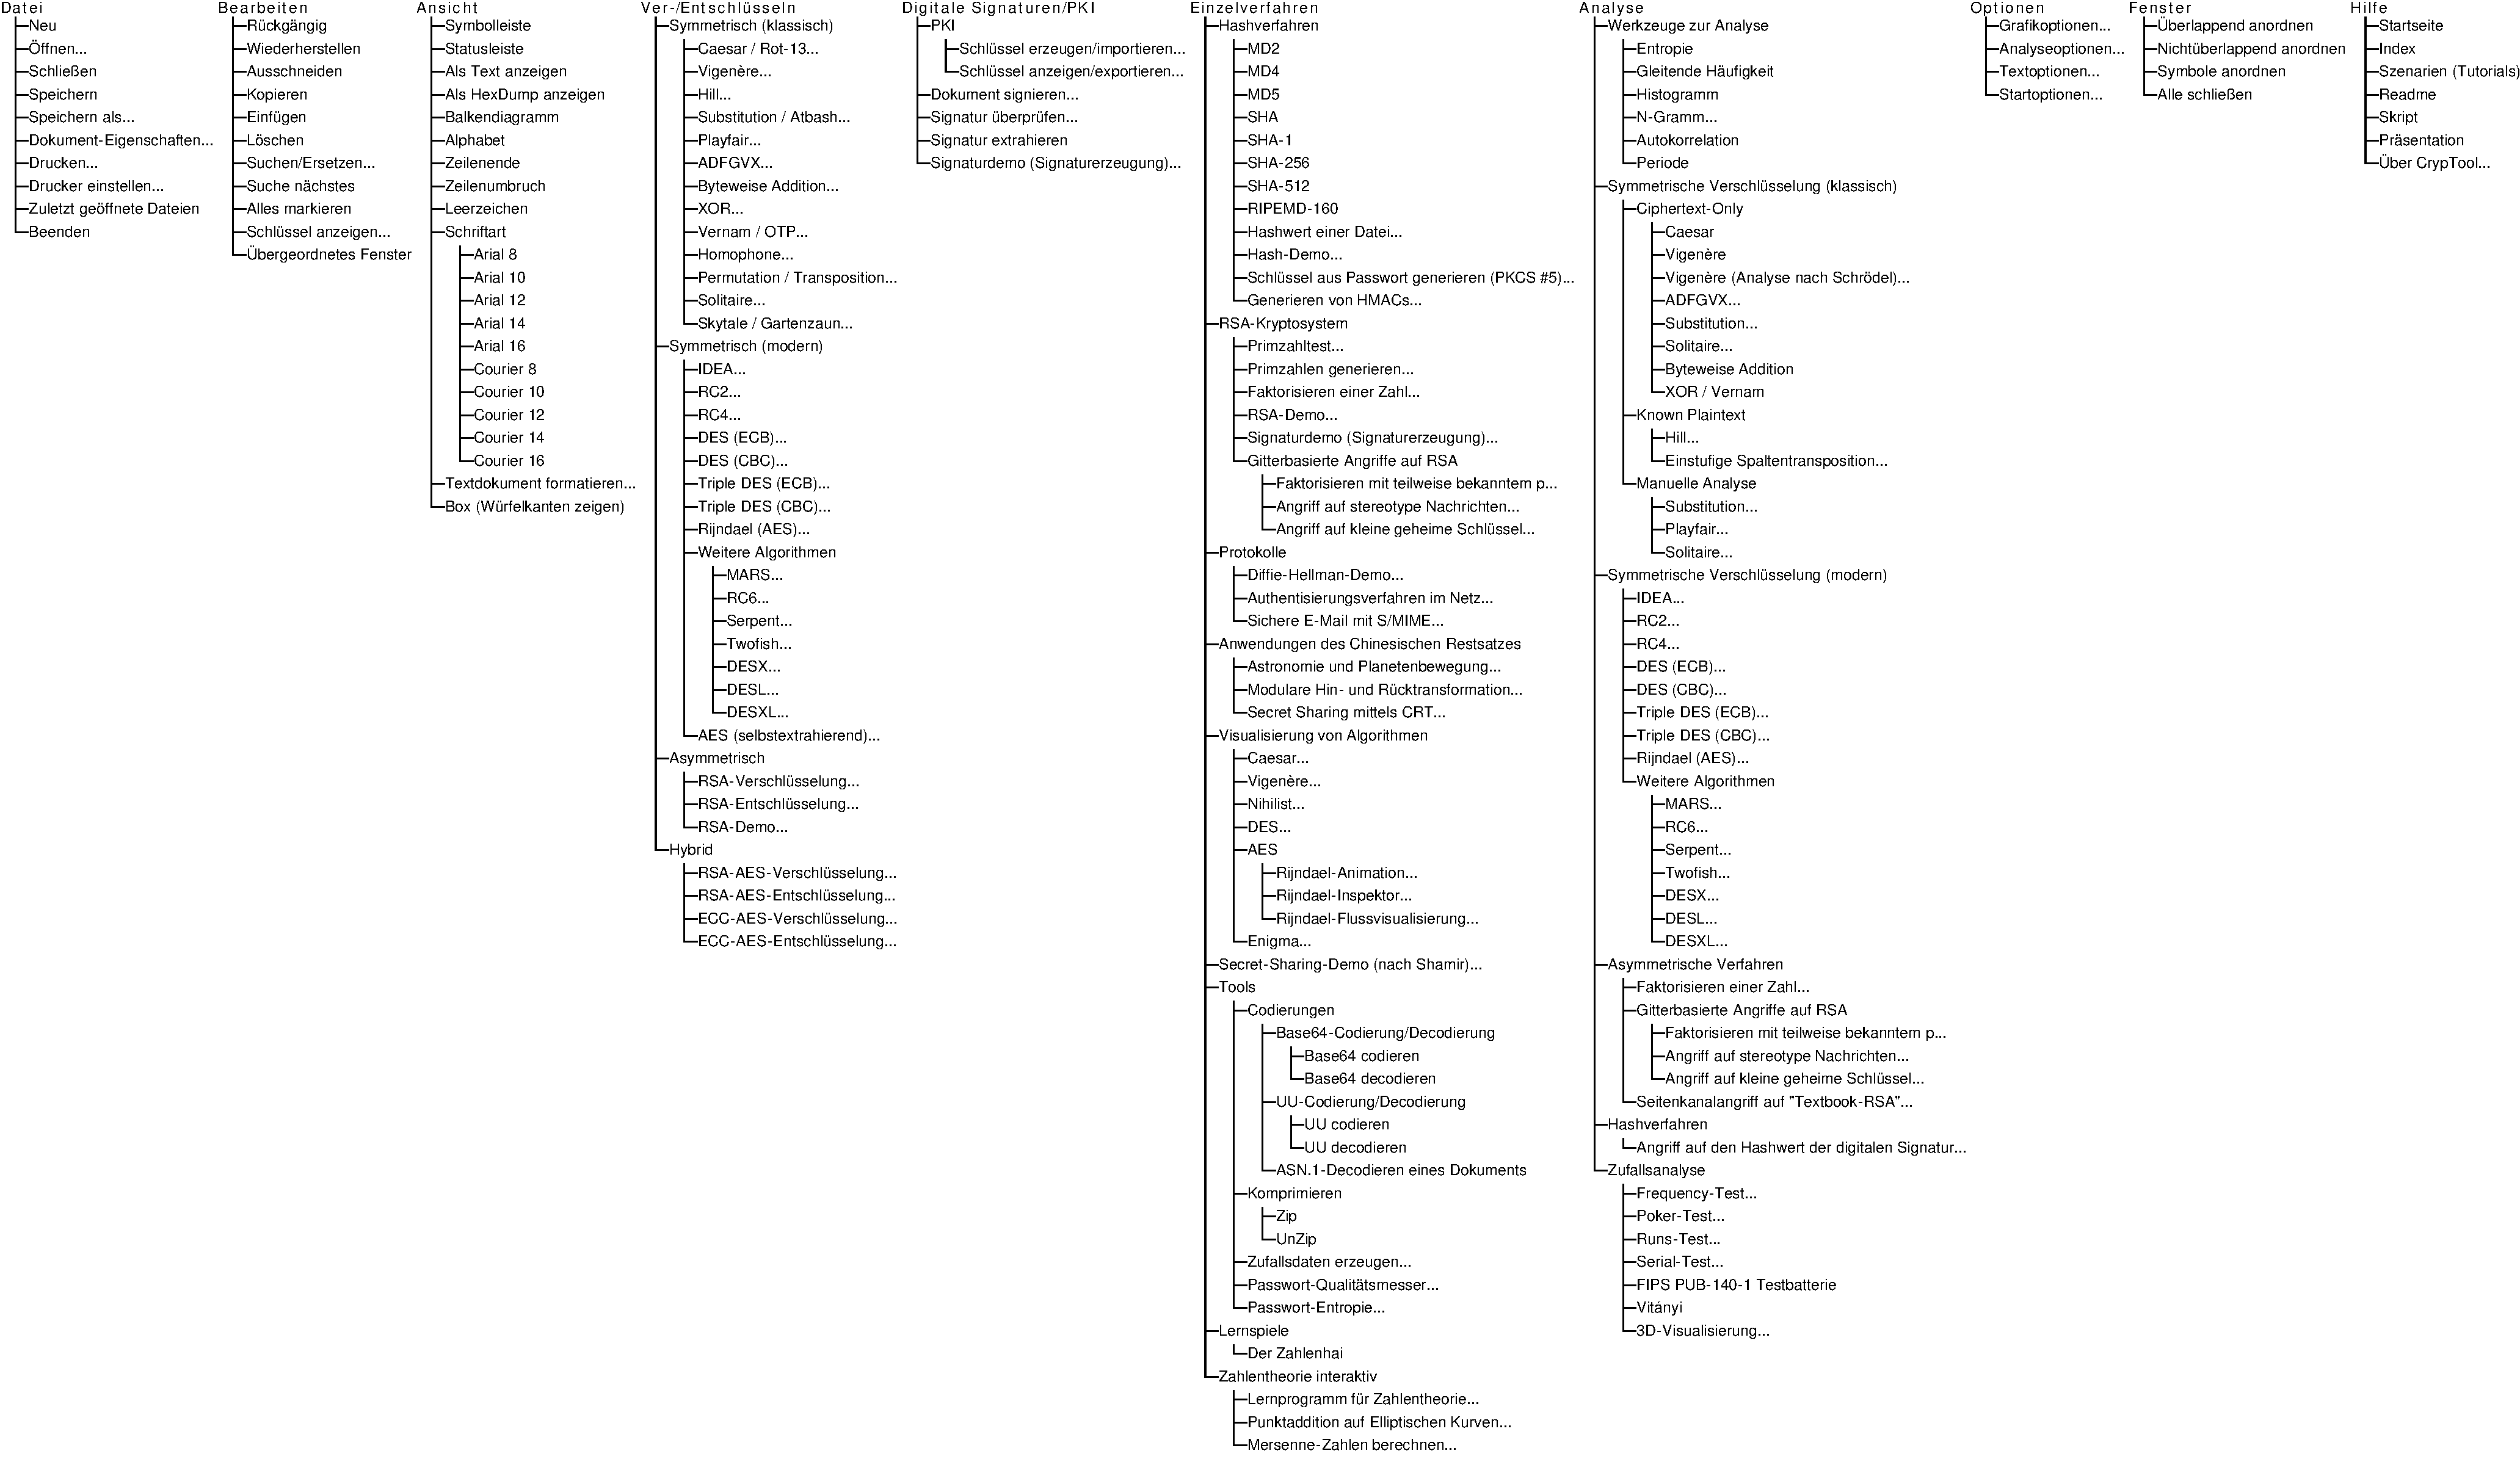
\includegraphics[scale=0.35, angle=270]
                {figures/CT1-menutree-de}
%viewport=rand-links? rand-unten breite hoehe [bezogen auf querformat]
%}
\hypertarget{appendix-figure-menu-overview-CT1}{}
\caption{Komplette �bersicht �ber den Men�-Baum von CT1 (CrypTool 1.4.31)} 
\label{appendix-figure-menu-overview-CT1}
\end{center}
\end{figure}
\clearpage




%--------------------------------------------------------------------
\newpage
%\enlargethispage{1cm}
\hypertarget{appendix-template-overview-CT2}{}
\section{CrypTool-2-Vorlagen}
\label{s:appendix-template-overview-CT2}

\noindent Dieser Anhang enth�lt auf den folgenden Seiten den Baum
mit allen Vorlagen in CrypTool 2\index{CrypTool 2}.\footnote{%
  Weitere Informationen zu CT2 finden Sie auf:
  \url{http://www.cryptool.org/de/ct2-documentation-de}
}

\noindent Beim Start von CT2 �ffnet sich das Startcenter.

%\clearpage
\begin{figure}[hb]
\begin{center}
%\vspace{-30pt}
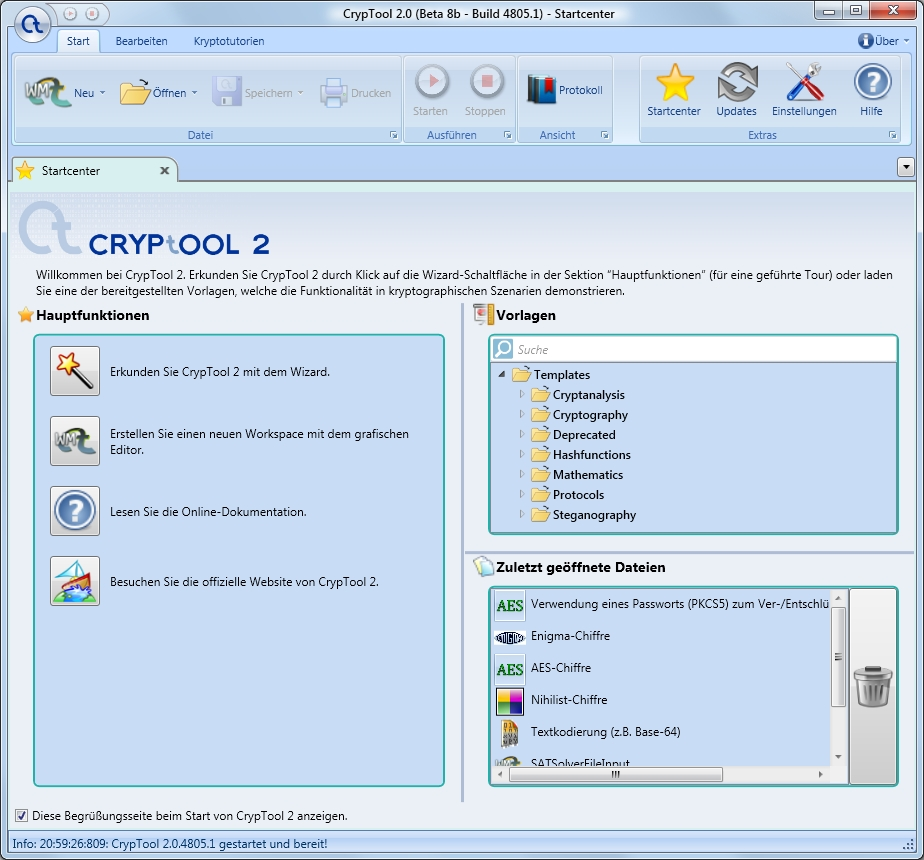
\includegraphics[scale=0.45, angle=0] {figures/CT2-Startcenter-de}
\hypertarget{Welcome-CT2}{}
\caption{Startcenter in CT2 (Beta 8b, Mai 2012)} 
\label{Welcome-Screenshot-CT2}
\end{center}
\end{figure}
%\clearpage

\noindent Darin hat man die Auswahl, die Funktionalit�t auf drei verschiedenen Wegen aufzurufen:
\begin{itemize}
   \item den Wizard: Er leitet einen gef�hrt zu den Funktionen.
   \item die Arbeitsfl�che, auf der man die Komponenten anhand der visuellen Programmierung\index{Visuelle Programmierung} selbst zusammenstellen kann.
   \item den Vorlagen-Baum, aus dem man fertige Workflows ausw�hlen kann.
 \end{itemize}

Der Wizard stellt Fragen zu dem gew�nschten Szenario (z.B. Base64-Codierung) und f�hrt einen dann zu den Funktionen. Das gew�hlte Szeanrio mit den eigenen Eingaben kann man anschlie�end auch als Vorlage abspeichern.

Auf die leere Arbeitsfl�che kann man aus der linken Navigationsleiste alle Komponenten ziehen und diese dann wie gew�nscht miteinander verbinden. Die implementierte Krypto-Funktionalit�t steckt vor allem in diesen Komponenten (z.B. Enigma, AES).

Im Vorlagen-Baum gibt es zu jeder Komponente mindestens eine Vorlage. Die angebotenen Vorlagen enthalten sofort lauff�hige komplette Workflows. Wenn man z.B. in der Vorlage zu AES seine Eingaben �ndert, sieht man dynamisch und sofort, wie sich Ausgaben entsprechend �ndern (wie z.B. durch Padding ein Block hinzukommt, wie sich das Chaining auswirkt, ...).

\clearpage
\begin{figure}[hb]
\begin{center}
\vspace{-30pt}
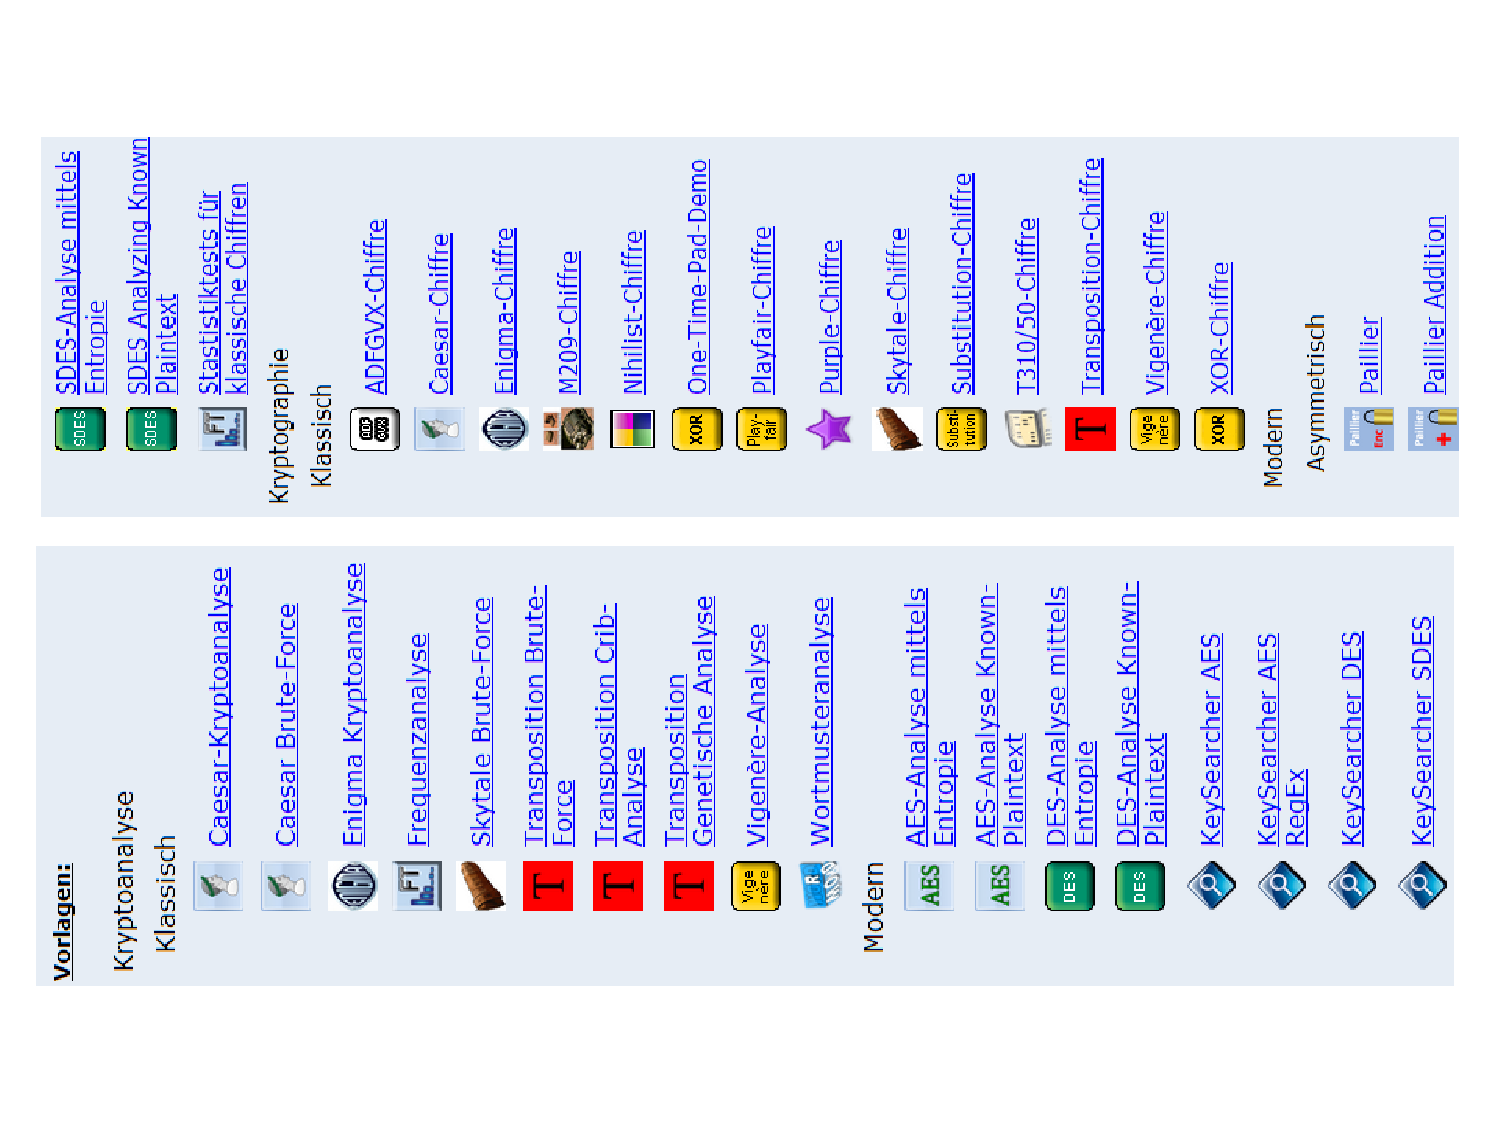
\includegraphics[scale=0.8, angle=270]
                {figures/CT2-templatetree-de-1}
\hypertarget{appendix-figure-template-overview-CT2}{}
\caption{Screenshot �ber den Template-Baum von CT2 (NB4882.1, Juli 2012), Teil 1} 
\label{appendix-figure-template-overview-CT2}
% \hypertarget{appendix-figure-template-overview-CT2}{}
\end{center}
\end{figure}
\clearpage





%--------------------------------------------------------------------
\newpage
%\enlargethispage{1cm}
\hypertarget{appendix-function-overview-JCT}{}
\section{JCrypTool-Funktionen}
\label{s:appendix-function-overview-JCT}

\noindent Dieser Anhang enth�lt auf den folgenden Seiten eine Liste aller
Funktionen in JCrypTool\index{JCrypTool}.\footnote{%
  Weitere Informationen zu JCT finden Sie auf:
  \url{http://www.cryptool.org/de/jct-machmit-de} \\
  Die Liste wurde mit Hilfe der CT-Portal-Webseite gewonnen.}

\noindent Beim ersten Start von JCT �ffnet sich das Willkommen-Fenster.

%\clearpage
\begin{figure}[hb]
\begin{center}
%\vspace{-30pt}
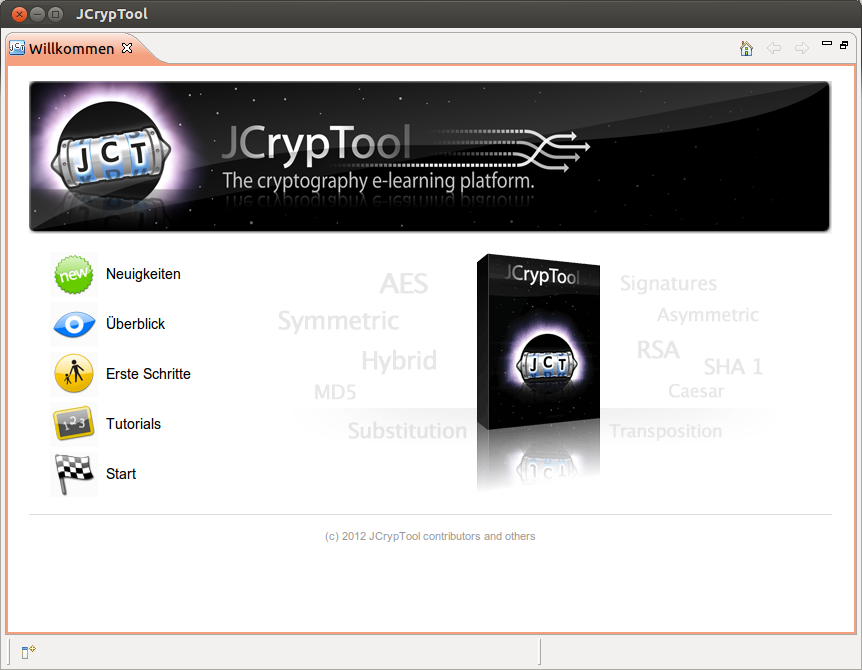
\includegraphics[scale=0.45, angle=0] {figures/JCT-Welcome-DE}
\hypertarget{Welcome-Screenshot-JCT}{}
\caption{Willkommen-Fenster in JCT (RC6, Juli 2012)} 
\label{Welcome-Screenshot-JCT}
\end{center}
\end{figure}
%\clearpage
Mit Klick auf ``Start'' kann man die verschiedenen Funktionen direkt nutzen.
Die in JCT implementierten Funktionen werden �ber zwei unterschiedliche Perspektiven angeboten:
\begin{itemize}
   \item Standard-Perspektive
   \item Funktional-Perspektive
 \end{itemize}

Alle Funktionen in der {\bf Standard-Perspektive} finden sich sowohl in den Men�s als
auch in der ``Krypto-Explorer'' genannten Navigationsleiste (rechts). Die Standard-Perspektive enth�lt alle wichtigen Verfahren (wie z.B. die klassische Transposition oder der moderne AES)  und viele Visualisierungen (z.B. Diffie-Hellman-Schl�sselaustausch oder Berechnungen auf Elliptischen Kurven).

Alle Funktionen der {\bf Funktional-Perspektive} finden sich in der ``Algorithmen'' genannten Navigationsleiste (in dieser Perspektive ebenfalls rechts). Die Funktional-Perspektive enth�lt alle Detaileinstellungen der verschiedenen Algorithmen und bietet insbesondere auch Algorithmen aus dem Bereich des Post-Quantum-Computings\index{Post-Quantum-Computing} an.

\clearpage
\begin{figure}[hb]
\begin{center}
\vspace{-30pt}
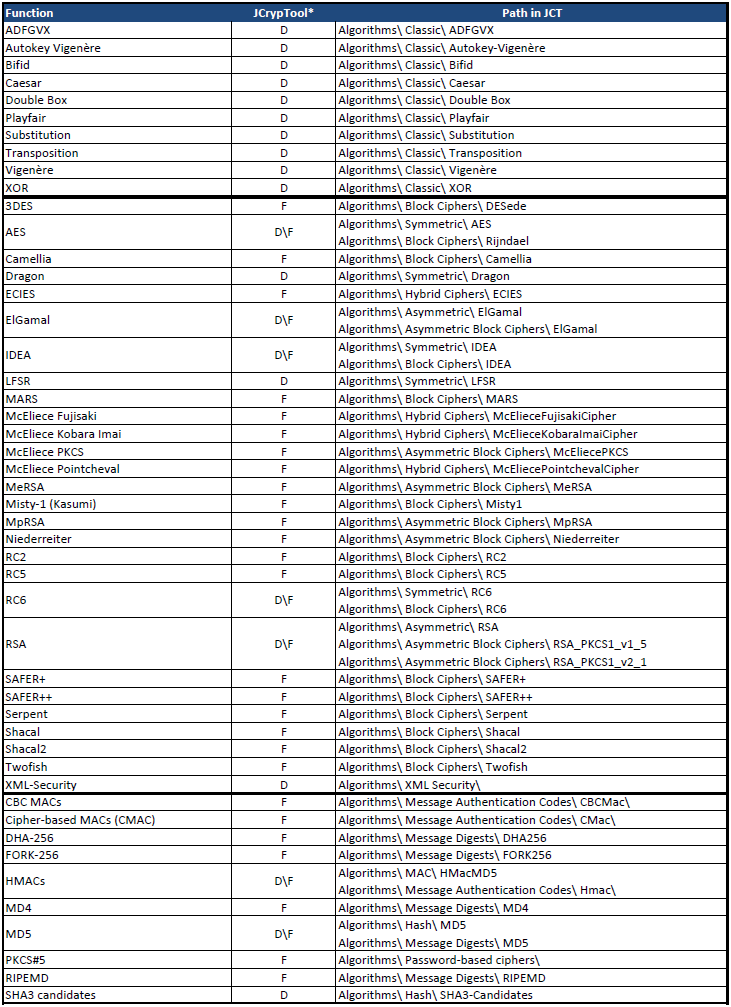
\includegraphics[scale=0.8, angle=0] {figures/JCT-functions-de-1}
\hypertarget{functions-overview-1-JCT}{}
\caption{Screenshot zu den Funktionen in JCT (RC6, Juli 2012), Teil 1} 
\label{functions-overview-1-JCT}
\end{center}
\end{figure}
\clearpage

\clearpage
\begin{figure}[hb]
\begin{center}
\vspace{-30pt}
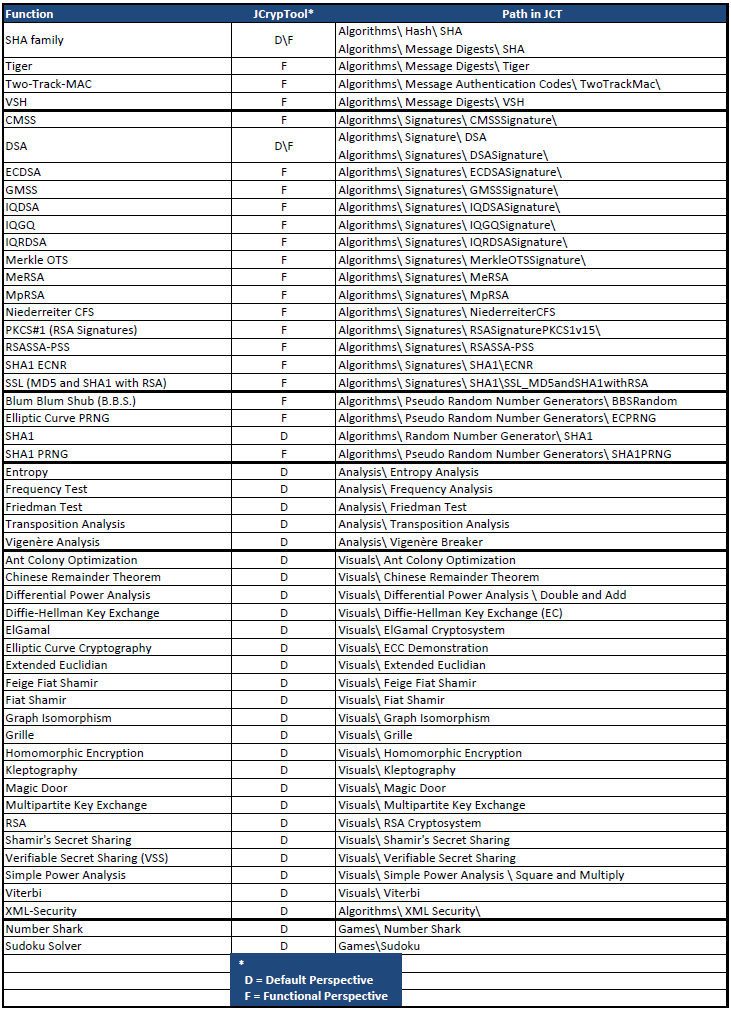
\includegraphics[scale=0.8, angle=0] {figures/JCT-functions-de-2}
\hypertarget{functions-overview-2-JCT}{}
\caption{Screenshot zu den Funktionen in JCT (RC6, Juli 2012), Teil 2} 
\label{functions-overview-2-JCT}
\end{center}
\end{figure}
\clearpage





%--------------------------------------------------------------------
\newpage
%\enlargethispage{1cm}
\hypertarget{appendix-function-overview-CTO}{}
\section{CrypTool-Online-Funktionen}
\label{s:appendix-function-overview-CTO}

\noindent Dieser Anhang enth�lt eine Liste aller
Funktionen in CrypTool-Online (CTO)\index{CrypTool-Online}.\footnote{%
  Weitere Informationen zu CTO finden Sie auf:
  \url{www.cryptool-online.org} \\
  Die Liste wurde mit Hilfe der Funktionsliste auf der CT-Portal-Webseite gewonnen:\\
  \url{http://www.cryptool.org/ctp-documentation-en/ctp-functions-en}}


%\noindent Die Einstiegsseite von CTO sieht so aus:
%\clearpage
%\begin{figure}[hb]
%\begin{center}
%\vspace{-30pt}
%\includegraphics[scale=0.45, angle=0] {figures/CTO-Welcome-DE}
%\hypertarget{Welcome-Screenshot-CTO}{}
%\caption{Einstiegsseite in CrypTool-Online (November 2012)} 
%\label{Welcome-Screenshot-CTO}
%\end{center}
%\end{figure}
%\clearpage


\noindent Der folgende Screenshot zeigt die auf CTO implementierten
Krypto-Funktionen:
\clearpage
\begin{figure}[hb]
\begin{center}
\vspace{-30pt}
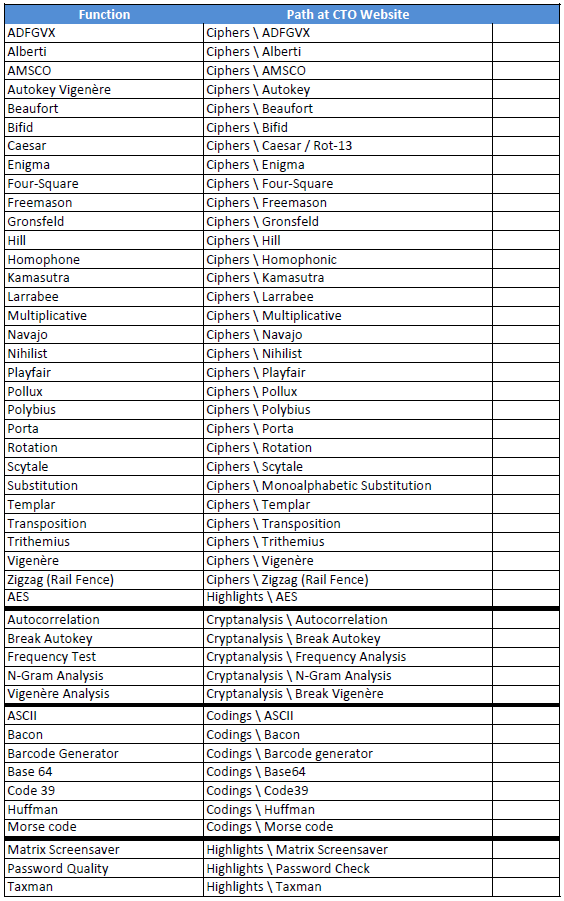
\includegraphics[scale=0.8, angle=0] {figures/CTO-functions-de-1}
\hypertarget{functions-overview-1-CTO}{}
\caption{Screenshot zu den Funktionen in CTO (November 2012)} 
\label{functions-overview-1-CTO}
\end{center}
\end{figure}
\clearpage

%\clearpage
%\begin{figure}[hb]
%\begin{center}
%\vspace{-30pt}
%\includegraphics[scale=0.8, angle=0] {figures/CTO-functions-de-2}
%\hypertarget{functions-overview-2-CTO}{}
%\caption{Screenshot zu den Funktionen in CTO (November 2012), Teil 2} 
%\label{functions-overview-2-CTO}
%\end{center}
%\end{figure}
%\clearpage


  \section{Autoren dieses Skripts}
\hypertarget{appendix-authors}{}\label{s:appendix-authors}

Dieser Anhang f"uhrt die Autoren des CrypTool-Skripts auf. Am Anfang jedes
Kapitels werden die Autoren angegeben, die zu diesem Kapitel beigetragen haben.

\begin{description}
\item[Bernhard Esslinger,] Initiator von CrypTool, Leiter IT Security in der Deutschen
Bank und Dozent an der Universit"at Siegen.
 
\item[Matthias B"uger,] Mitautor des Kapitels ``Elliptische Kurven'',
Research Analyst bei der Deutschen Bank, verantwortlich f"ur den Deutsche Bank
Kryptographie-Standard.

\item[Bartol Filipovic,] urspr"unglicher Autor der
Elliptische-Kurven-Implementierung in CrypTool und des entsprechenden Kapitels
in diesem Skript.

\item[Henrik Koy, ] Hauptentwickler und Koordinator der CrypTool-Entwicklung
seit Version 1.3, Reviewer des Skripts und \TeX{}-Guru, Projektleiter IT bei der
Deutschen Bank.

\item[Roger Oyono, ] Implementierer des Faktorisierungs-Dialogs in CrypTool und urspr"unglicher Autor des Kapitels "`Die mathematischen Ideen hinter der modernen Kryptographie"'.

\item[J"org Cornelius Schneider,] Design und Support von CrypTool,
Kryptographie-Enthusiast und Projektleiter IT bei der Deutschen Bank.

\end{description}


  % $Id:
% !Mode:: "TeX:DE"    % Setting document mode and submode for WinEdt
% ..............................................................................
%             W A S  I S T  S A G E M A T H  ?
% ~~~~~~~~~~~~~~~~~~~~~~~~~~~~~~~~~~~~~~~~~~~~~~~~~~~~~~~~~~~~~~~~~~~~~~~~~~~~~~

\newpage
\hypertarget{appendix-using-sage}{}
\section{Kurzeinf�hrung in das CAS SageMath}
\label{s:appendix-using-sage}
\index{SageMath}
\index{SageMath!Programmbeispiele}

%% Unter \url{https://wiki.sagemath.org/combinat} gibt es Weiterentwicklung on-top of Sage.
%% Diese kommen meist nach und nach ins offizielle Sage rein.


Dieses Buch enth�lt zahlreiche mit SageMath erstellte Programmbeispiele. SageMath ist
ein Open-Source Computer-Algebra-System (CAS), das f�r Lehre, Studium und Forschung
eingesetzt wird.
SageMath kombiniert viele hochwertige Open-Source-Packete\footnote{%
Einen Eindruck von der Gr��e von SageMath erh�lt man, wenn man es selbst compiliert:
Die heruntergeladenen Sourcen von SageMath 4.1 brauchten zur Compilierung auf einem
durchschnittlichen Linux-PC rund 5 h (inklusive aller Bibliotheken).
Danach nahm es 1,8 GB Plattenplatz ein.
}
und liefert den Zugang zu deren Funktionalit�t �ber ein gemeinsames, auf der
Programmiersprache Python\index{Python} basierendes Interface\footnote{%
Es gibt auch ein relativ einfaches Interface f�r die Sprache C, genannt Cython,
mit der man eigene Funktionen in SageMath stark beschleunigen kann.\\
Siehe \url{http://openwetware.org/wiki/Open_writing_projects/Sage_and_cython_a_brief_introduction}.
}.

\noindent SageMath kann man auf vielf�ltige Weise nutzen:
als m�chtigen Taschenrechner; als Tool f�r das Mathematikstudium;
oder als Programmier-Umgebung, um Algorithmen zu prototypen oder um Forschung im
Bereich der algorithmischen Aspekte der Mathematik zu betreiben.

\noindent Einen schnellen Einstieg bieten z.B. die Referenzen in dieser Fu�note%
\footnote{%
\noindent\hangindent=6pt\makebox[6pt][l]{-}\glqq Einladung zu Sage\grqq~von David Joyner, letztes Update 2009,\\
  \url{http://sage.math.washington.edu/home/wdj/teaching/calc1-sage/an-invitation-to-sage.pdf}

\noindent\hangindent=6pt\makebox[6pt][l]{-}\glqq The SDSU Sage Tutorial\grqq,\\
  \url{http://www-rohan.sdsu.edu/~mosulliv/sagetutorial/}\\
  \url{http://www-rohan.sdsu.edu/~mosulliv/sagetutorial/sagecalc.html}

  \noindent\hangindent=6pt\makebox[6pt][l]{-}{\glqq SAGE For Newbies\grqq~von Ted Kosan, 2007,\\
  \url{http://sage.math.washington.edu/home/tkosan/newbies_book/sage_for_newbies_v1.23.pdf}}
   % Leerzeile am Ende n�tig, sonst hat die letzte Zeile KEINEN h�ngenden Einzug?! (TODO_LaTeX)
   %%%% Aber das auch unsch�n.
}.

\noindent Die offizielle SageMath Online-Dokumentation\footnote{%
  Die entsprechenden offiziellen PDF-Dokuments k�nnen herunter geladen werden von\\
  \url{http://www.sagemath.org/help.html}, \url{http://www.sagemath.org/doc} und \url{http://planet.sagemath.org}.
} finden Sie unter: \url{http://www.sagemath.org}.


\noindent Es gibt inzwischen viele PDF- und HTML-Dokumente �ber SageMath, so dass wir als guten Startpunkt nur einige wenige nennen\footnote{%
- \glqq Bibliothek\grqq: {\centering \url{http://www.sagemath.org/library.html}},\\
- \glqq Dokumentationsprojekt\grqq:
  {\centering \url{http://wiki.sagemath.org/DocumentationProject}},\\
- \glqq Lehrmaterial\grqq: {\centering \url{http://wiki.sagemath.org/Teaching_with_SAGE}}.
}.

\noindent Auch beim Studium der Kryptologie k�nnen fertige SageMath-Module genutzt
werden\footnote{%
\noindent\hangindent=6pt\makebox[6pt][l]{-}�berblick,
   welche Kryptographie momentan in SageMath enthalten ist:\\
   \url{http://www.sagemath.org/doc/reference/sage/crypto/}

\noindent\hangindent=6pt\makebox[6pt][l]{-}Diskussionen
   �ber Lernaspekte beim Entwickeln weiterer Krypto-Module in SageMath:\\
   \url{http://groups.google.com/group/sage-devel/browse_thread/thread/c5572c4d8d42d081}
% Leerzeile bei den Aufz�hlungen am Ende n�tig, damit die 2. Zeile (Url) h�ngenden Einzug hat.
% ABER: Bei der letzten Aufz�hlung f�hrt Leerzeile zu leerer Zeile (was nicht gewollt ist) und die letzte Url hat trotzdem keinen h�ngenden Einzug! (TODOTODO)
}.

\noindent Umfangreiche Kryptographie-Einf�hrungen finden sich in der folgenden Fu�note\footnote{%
\noindent\hangindent=6pt\makebox[6pt][l]{-}Ein fertiger Kryptographie-Kurs von David Kohel,
  der SageMath nutzt, aus 2008:\\
  {\centering \url{http://www.sagemath.org/files/kohel-book-2008.pdf} }\\
  bzw. derselbe Kurs in einer neueren Fassung (2015)\\
  {\centering \url{http://iml.univ-mrs.fr/~kohel/tch/M2-CryptoSymetrique/crypto.pdf} }.

\noindent\hangindent=6pt\makebox[6pt][l]{-}\glqq Introduction to Cryptography with
  Open-Source Software\grqq, ein hervorragendes Buch von Alasdair McAndrew, CRC, 2011
  %% TODO: Wenn die eine Zeile l�nger, beginnt sie doch wieder ganz vorne!
}.


% ---------------------------------------------------------------------------
\section*{SageMath-Benutzerschnittstellen}
SageMath ist kostenlos und kann von folgender Webseite herunter geladen werden:
\begin{center}
  \url{http://www.sagemath.org} \\
\end{center}
Standardm��ig nutzt man die SageMath-{\bf Kommandozeile} als Interface, wie im
folgenden Bild~\ref{fig:sage_cmd_interfaces} zu sehen ist.
Es gibt jedoch auch ein grafisches Benutzerinterface f�r diese Software
in Form des SageMath-Notebooks (siehe Bild~\ref{fig:sage_gui_interfaces}).
Und schlie�lich kann man SageMath-{\bf Notebooks}\footnote{%
Weitere Details zu SageMath-Notebooks finden Sie in
Kapitel~\ref{ec:Sage_Massierer}
(\glqq \nameref{ec:Implementing-for-Education}\grqq
  $\Rightarrow$ \glqq \nameref{ec:Sage_Massierer}\grqq).
                      }
auch online auf verschiedenen Servern nutzen, ohne SageMath lokal zu installieren, z.B.:
\begin{center}
\url{http://sagecell.sagemath.org/} oder \\
\url{https://cocalc.com/}
\end{center}

SageMath l�uft unter den Betriebssystemen Linux, Mac OS X und Windows.
Auf der Windows-Plattform l�uft die komplette SageMath-Distribution momentan
nur als ein VMware-Image.

\begin{figure}[!htpb]
\centering
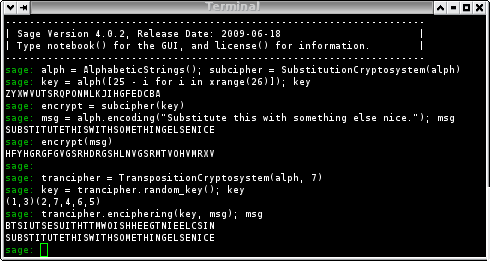
\includegraphics[scale=0.6]{figures/sage-cmd}
\caption{SageMath-Kommandozeilen-Interface}
\label{fig:sage_cmd_interfaces}
\end{figure}

\begin{figure}[!htpb]
\centering
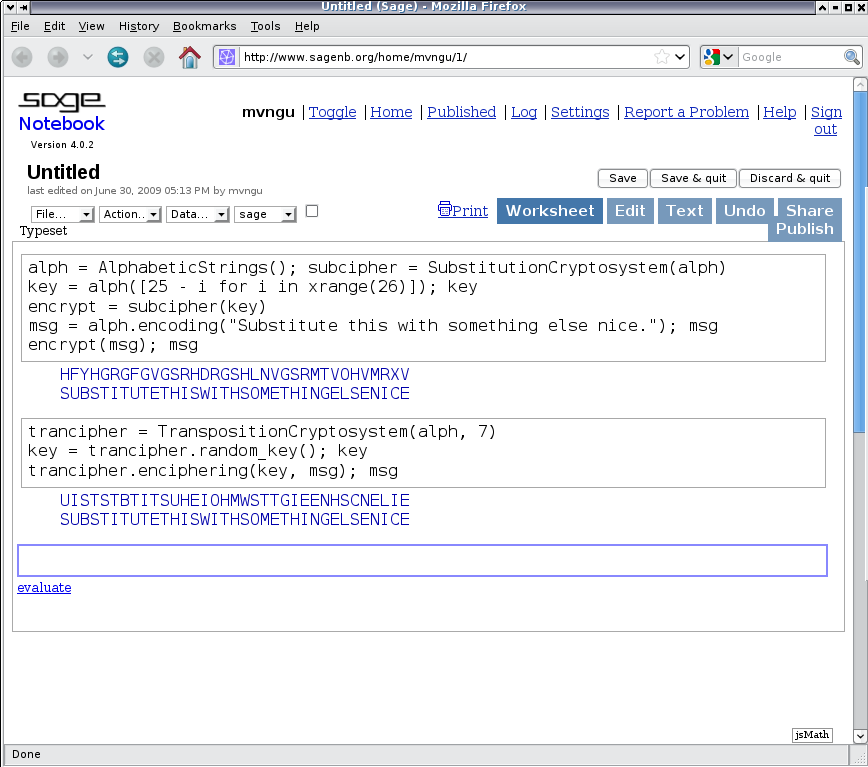
\includegraphics[scale=0.4]{figures/sage-gui}
\caption[SageMath-Notebook-Interface]{SageMath-Notebook-Interface\footnotemark}
\label{fig:sage_gui_interfaces}
\end{figure}

\footnotetext{%
Um das grafische SageMath-Interface lokal zu starten, muss man auf der SageMath-Kommandozeile
\verb#notebook()# eingeben. Danach startet der eingestellte Browser (Iceweasel,
Firefox, IE, ...) z.B. mit der URL \textit{http://localhost:8000}.
}



% ---------------------------------------------------------------------------
\newpage
\section*{Hilfe beim Benutzen von SageMath}

Wenn man SageMath auf der Kommandozeile startet, erh�lt etwas wie die folgenden Zeilen:
%
\begin{Verbatim}%
[fontsize=\footnotesize]
mnemonic:~$ sage
----------------------------------------------------------------------
| Sage Version 4.1, Release Date: 2009-07-09                         |
| Type notebook() for the GUI, and license() for information.        |
----------------------------------------------------------------------

sage: help
Type help() for interactive help, or help(object) for help about object.
sage:
sage:
sage: help()

Welcome to Python 2.6!  This is the online help utility.

If this is your first time using Python, you should definitely check out
the tutorial on the Internet at http://docs.python.org/tutorial/.

Enter the name of any module, keyword, or topic to get help on writing
Python programs and using Python modules.  To quit this help utility and
return to the interpreter, just type "quit".

To get a list of available modules, keywords, or topics, type "modules",
"keywords", or "topics".  Each module also comes with a one-line summary
of what it does; to list the modules whose summaries contain a given word
such as "spam", type "modules spam".
\end{Verbatim}
%
Viele weitere Hilfen gibt es als offizielle SageMath-Dokumentation, die mit jedem
Release von SageMath verteilt wird~(siehe Bild~\ref{fig:sage_standard_doc}).
%
\begin{figure}[!htpb]
\centering
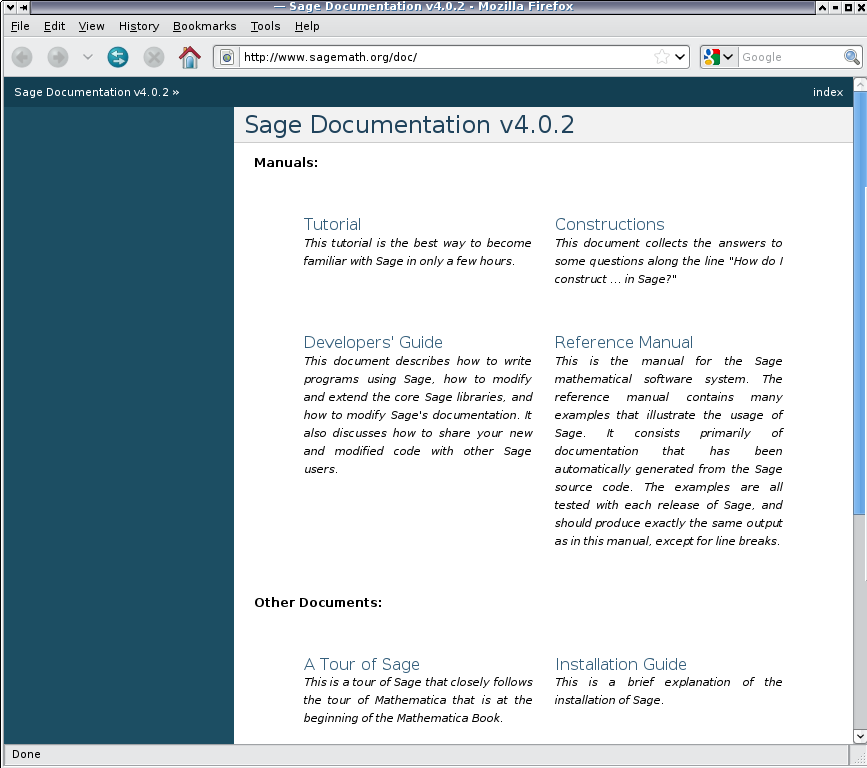
\includegraphics[scale=0.4]{figures/sage-online-doc}
\caption{Die Standard-Dokumentation von SageMath}
\label{fig:sage_standard_doc}
\end{figure}
%
Zur offiziellen SageMath-Standard-Dokumentation geh�ren folgende Dokumente:

\begin{itemize}
\item Tutorial --- Das Tutorial ist f�r SageMath-Einsteiger.
  Es ist daf�r gedacht, sich in ein bis drei Stunden mit den
  wichtigsten Funktionen vertraut zu machen.

\item Constructions --- Dieses Dokument ist im Stil eines \glqq Kochbuchs\grqq~mit
  einer Sammlung von Antworten auf Fragen zur Konstruktion von SageMath-Objekten.

\item Developers' Guide --- Dieser F�hrer ist f�r Entwickler, die selbst SageMath
  mit weiter entwickeln wollen. Enthalten sind darin z.B. Hinweise zum
  Stil und zu Konventionen beim Programmieren, zur Modifikation von
  SageMath-Kern-Bibliotheken oder von SageMath-Standard-Dokumentation, und zum Code-Review
  und zur Software-Verteilung.

\item Reference Manual --- Dieses Handbuch enth�lt die komplette Dokumentation
  aller wichtigen SageMath-Funktionen. Zu jeder Klassen-Beschreibung gibt es
  mehrere Code-Beispiele. Alle Code-Beispiele im Referenz-Handbuch werden
  bei jedem neuen SageMath-Release getestet.

\item Installation Guide --- Dieser F�hrer erkl�rt, wie man SageMath auf
  verschiedenen Plattformen installiert.

\item A Tour of Sage --- Diese Tour durch SageMath zeigt exemplarisch verschiedene
  Funktionen, die f�r Einsteiger sinnvoll sind.

\item Numerical Sage --- Dieses Dokument f�hrt Werkzeuge auf, die in SageMath
  f�r numerische Mathematik verf�gbar sind.

\item Three Lectures about Explicit Methods in Number Theory Using
  Sage --- Drei Vorlesungen �ber Methoden der Zahlentheorie, die explizit
  SageMath nutzen. Dieses Dokument zeigt wie man mit SageMath Berechnungen in
  fortgeschrittener Zahlentheorie durchf�hrt.
\end{itemize}

\noindent Von der SageMath-Kommandozeile erh�lt man eine Liste aller verf�gbaren Kommandos
(Funktionsnamen etc.), die ein bestimmtes Muster haben, wenn man die ersten Zeichen tippt,
und dann die \glqq Tab\grqq-Taste dr�ckt:
%
\begin{Verbatim}%
[fontsize=\footnotesize]
sage: Su[TAB]
Subsets                   Subwords                  SuzukiGroup
SubstitutionCryptosystem  SupersingularModule
\end{Verbatim}
%
Wenn man den genauen Namen eines Kommandos kennt, kann man die \texttt{help}-Funktion
nutzen oder das Fragezeichen \glqq ?\grqq~anf�gen, um weitere Informationen zu
diesem Kommando zu erhalten.  Zum Beispiel liefert das Kommando
\texttt{help(SubstitutionCryptosystem)} die Dokumentation zur der eingebauten
Klasse \texttt{SubstitutionCryptosystem}. Mit dem Fragezeichen erhalten wir die
Dokumentation zu dieser Klasse auf folgende Weise:
%
\begin{Verbatim}%
[fontsize=\footnotesize]
sage: SubstitutionCryptosystem?
Type:type
Base Class:<type 'type'>
String Form:<class 'sage.crypto.classical.SubstitutionCryptosystem'>
Namespace:Interactive
File:/home/mvngu/usr/bin/sage-3.4.1/local/lib/python2.5/site-packages/sage/crypto/classical.py
Docstring:

        Create a substitution cryptosystem.

        INPUT:

        - ``S`` - a string monoid over some alphabet

        OUTPUT:

        - A substitution cryptosystem over the alphabet ``S``.

        EXAMPLES::

            sage: M = AlphabeticStrings()
            sage: E = SubstitutionCryptosystem(M)
            sage: E
            Substitution cryptosystem on Free alphabetic string monoid
            on A-Z
            sage: K = M([ 25-i for i in range(26) ])
            sage: K
            ZYXWVUTSRQPONMLKJIHGFEDCBA
            sage: e = E(K)
            sage: m = M(``THECATINTHEHAT'')
            sage: e(m)
            GSVXZGRMGSVSZG

        TESTS::

            sage: M = AlphabeticStrings()
            sage: E = SubstitutionCryptosystem(M)
            sage: E == loads(dumps(E))
            True
\end{Verbatim}
%
\vspace{30pt}
Weitere Unterst�tzung f�r spezifische Probleme gibt es in den Archiven der
\texttt{sage-support} Mailing-Liste unter
%
\begin{center}
  \url{http://groups.google.com/group/sage-support}
\end{center}




% ---------------------------------------------------------------------------
\newpage
\section*{Beispiele f�r in SageMath eingebaute mathematische Funktionen}

Hier sind ein paar kleine Beispiele\footnote{%
Diese Beispiele stammen aus dem Blog von Dr. Alasdair McAndrew, Victoria University,\\
\url{http://amca01.wordpress.com/2008/12/19/sage-an-open-source-mathematics-software-system}}
(alle f�r das Kommandozeilen-Interface -- zur einfacheren Nutzung), um zu sehen,
was man mit SageMath machen kann:

\begin{sagecode}
\begin{Verbatim}%
[fontsize=\footnotesize]
# * Analysis (Infinitesimalrechnung):
    sage: x=var('x')
    sage: p=diff(exp(x^2),x,10)*exp(-x^2)
    sage: p.simplify_exp()
     1024 x^10 + 23040 x^8 + 161280 x^6 + 403200 x^4 + 302400 x^2 + 30240

# * Lineare Algebra:
    sage: M=matrix([[1,2,3],[4,5,6],[7,8,10]])
    sage: c=random_matrix(ZZ,3,1);c
     [ 7 ]
     [-2 ]
     [-2 ]
    sage: b=M*c
    sage: M^-1*b
     [ 7 ]
     [-2 ]
     [-2 ]

# * Zahlentheorie:
    sage: p=next_prime(randint(2^49,2^50));p
      1022095718672689
    sage: r=primitive_root(p);r
      7
    sage: pl=log(mod(10^15,p),r);pl
      1004868498084144
    sage: mod(r,p)^pl
      1000000000000000

# * Endliche K�rper (\url{http://de.wikipedia.org/wiki/Endlicher_K%C3%B6rper}):
    sage: F.<x>=GF(2)[]
    sage: G.<a>=GF(2^4,name='a',modulus=x^4+x+1)
    sage: a^2/(a^2+1)
      a^3 + a
    sage: a^100
      a^2 + a + 1
    sage: log(a^2,a^3+1)
      13
    sage: (a^3+1)^13
      a^2
\end{Verbatim}
\caption{Einige kleine Beispiele in SageMath aus verschiedenen Gebieten der Mathematik}
\end{sagecode}



% ---------------------------------------------------------------------------
\newpage
\section*{Programmieren mit SageMath}

Wenn man ein CAS (Computer-Algebra-System) nutzt, schreibt man zu Beginn einzelne
Befehle in die Kommandozeile wie im obigen Beispiel\footnote{%
  Standardm��ig wird SageMath-Code auch so pr�sentiert: Dabei beginnen die Zeilen
  mit  \glqq sage:\grqq~und \glqq ...\grqq.
  \begin{Verbatim}%
  [fontsize=\footnotesize]
  sage: m = 11
  sage: for a in xrange(1, m):
  ....:     print [power_mod(a, i, m) for i in xrange(1, m)]
  ....:
  \end{Verbatim}

  \noindent Auch dieses Skript benutzt normalerweise die obige Konvention, um
  SageMath-Code zu pr�sentieren, solange der Code nicht aus einer SageMath-Skriptdatei kommt.
  Wenn man den SageMath-Code aus diesem Skript kopiert und per Paste auf der SageMath-Kommandozeile
  wieder einf�gt, sollte man \glqq sage:\grqq~und \glqq ...\grqq~ weglassen
  (obwohl das Kommandozeilen-Interface in den meisten F�llen mit diesen Pr�fixen
  korrekt umgehen kann).}.

Wenn man eigene Funktionen entwickelt, sie �ndert und aufruft, dann ist es viel einfacher,
die Entwicklung in einem eigenen Editor vorzunehmen, den Code als SageMath-Skriptdatei zu
speichern und die Funktionen nicht-interaktiv auf der Kommandozeile auszuf�hren.
Beide Arten, Code zu entwickeln, wurden in
Kapitel \ref{CM_Sage_samples} (\glqq \nameref{CM_Sage_samples}\grqq),
Kapitel \ref{PaP_Sage_samples} (\glqq \nameref{PaP_Sage_samples}\grqq),
Kapitel \ref{primes:_Appendix_Sage-Samples} (\glqq \nameref{primes:_Appendix_Sage-Samples}\grqq)
und in Kapitel \ref{NumberTheory_Appendix_E} (\glqq\nameref{NumberTheory_Appendix_E}\grqq)
angewandt.

\noindent Um SageMath-Code in einem eigenen Editor zu entwickeln und zu testen, gibt es zwei
n�tzliche Befehle: \verb!load()! und \verb!attach()!\footnote{%
Vergleiche das SageMath-Tutorial �ber Programmierung, Kapitel
\glqq Loading and Attaching Sage files\grqq,\\
\url{http://doc.sagemath.org/html/en/tutorial/programming.html}.}.\\
Angenommen Sie haben die folgende Funktions-Definition:
\begin{Verbatim}%
   [fontsize=\footnotesize]
   def function(var1):
       r"""
       DocText.
       """
       ...
       return (L)
\end{Verbatim}
\noindent die in der Datei \texttt{primroots.sage} gespeichert wurde.

\noindent Um diese Funktion in SageMath zu laden (und syntaktisch gleich zu testen),
wird der Befehl \verb!load()! benutzt:

\texttt{sage: load primroots.sage}

\noindent Danach kann man auf der Kommandozeile alle Variablen und Funktionen
nutzen, die im Sage\-Math-Skript definiert wurden\footnote{%
Anmerkungen:

\noindent\hangindent=6pt\makebox[6pt][l]{-}Bitte keine Leerzeichen
oder White Spaces im Dateinamen.

\noindent\hangindent=6pt\makebox[6pt][l]{-}Es empfiehlt sich,
der SageMath-Skriptdatei die Datei-Extension
\glqq .sage\grqq~statt \glqq .py\grqq~zu geben.
Hat ein SageMath-Skript die Dateinamens-Endung \glqq .sage\grqq, dann wird
beim Laden der Datei in SageMath auch gleich die normale SageMath-Umgebung mit geladen,
um die Syntax zu pr�fen. Genauso funktioniert es, wenn man ein SageMath-Skript direkt
von einer Bash-Shell aufruft mit~~\texttt{\$ sage primroots.sage}.

\noindent\hangindent=6pt\makebox[6pt][l]{-}Beim Laden des obigen
SageMath-Skripts wird es von SageMath zuerst geparst, und dann
in eine andere Datei namens \glqq primroots.py\grqq~kopiert. SageMath erg�nzt
dann alle notwendigen Variablen in \glqq primroots.py\grqq~und alle Import-Statements.
Somit wird das SageMath-Skript genauso ausgef�hrt, als h�tte man die Befehle einzeln
auf der Kommandozeile eingetippt. Ein bedeutender Unterschied ist,
dass alle Ausgaben ein \verb!print!~ben�tigen.

}.

Normalerweise editiert man ein eigenes SageMath-Skript wieder und m�chte dann den
Inhalt des ge�nderten Skripts wieder in SageMath laden. Daf�r kann man den Befehl
\verb!attach()! nutzen (man kann auch direkt nach dem \verb!load()!
das \verb!attach()! aufrufen, und nicht erst, wenn man das Skript �ndert;
man kann \verb!load()! sogar weglassen, da dies in \verb!attach()! enthalten ist):

\texttt{sage: attach primroots.sage}

Nun kann man das SageMath-Skript �ndern und die ge�nderte Funktionsdefinition
wird -- solange man die SageMath-Session nicht beendet -- beim n�chsten Enter
in SageMath geladen (und syntaktisch gleich gepr�ft). Diese Neuladen passiert
vollkommen automatisch. Der Befehl attach() l�sst SageMath also permanent die
genannte Datei auf �nderungen �berwachen. Damit spart man sich das Kopieren
und Pasten zwischen dem eigenen Texteditor und dem SageMath-Kommandozeilen-Interface.

Hier ist ein Bild, das SageMath-Code im Editor GVIM zeigt -- mit aktiviertem
Syntax-Highlighting (siehe Bild~\ref{fig:sage-highlighted-code-in-editor}).
%
\begin{figure}[!htpb]
\centering
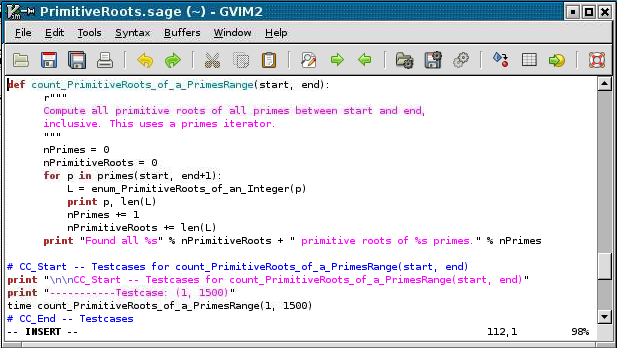
\includegraphics[scale=0.7]{figures/sage-highlighted-code-in-editor}
\caption{SageMath-Beispiel in einem Editor mit aktiviertem Code-Highlighting}
\label{fig:sage-highlighted-code-in-editor}
\end{figure}

\vspace{20pt}
Falls man die Ausgabe einer attachten Datei so angezeigt haben m�chte,
wie wenn man die Einzelbefehle direkt auf der Kommandozeile eingibt
(also nicht nur das, was per \verb!print! ausgegeben wird),
kann man den Befehl \verb!iload()! verwenden:
Jede Zeile wird dann einzeln geladen. Um die n�chste Zeile zu laden,
muss man die \verb!Enter!-Taste dr�cken. Das muss man so lange wiederholen,
bis alle Zeilen des SageMath-Skripts in die SageMath-Session geladen sind.

\texttt{sage: iload primroots.sage}


% \vspace{30pt}
\newpage
\noindent Weitere Hinweise:
\begin{itemize}
  \item Abfrage der Version Ihrer SageMath-Umgebung mit: \texttt{version()}
  \item Um sich schnell die SageMath-Programmbeispiele in diesem Skript anzusehen, k�nnen Sie
    \begin{itemize}
      \item im Index nach \verb#SageMath -> Programmbeispiele# schauen, oder
      \item sich im Anhang das \glqq \nameref{sc:List-of-Sage-Code-Examples}\grqq~ansehen.
    \end{itemize}
  \item Die SageMath-Beispiele in diesem Skript werden mit CrypTool ausgeliefert.\\
        Weitere Details am Ende der �bersicht
        \glqq \nameref{sc:List-of-Sage-Code-Examples}\grqq.
\end{itemize}



\end{appendix}

% This is set up to run with pdflatex.
%---------The file header---------------------------------------------
% \documentclass[a4paper,12pt]{book}

% \usepackage[english]{babel} %language selection
% \selectlanguage{english}

% \pagenumbering{arabic}

% \usepackage{hyperref}
% \hypersetup{colorlinks,
%            citecolor=black,
%            filecolor=black,
%            linkcolor=black,
%            urlcolor=black,
%            bookmarksopen=true,
%            pdftex}

% \hfuzz = .6pt % avoid black boxes

% \begin{document}
%---------------------------------------------------------------------
\chapter*{\rlap{GNU Free Documentation License}}
% \phantomsection  % so hyperref creates bookmarks
\addcontentsline{toc}{chapter}{GNU Free Documentation License}
%\label{label_fdl}

\begin{center}

       Version 1.3, 3 November 2008


 Copyright \copyright{} 2000, 2001, 2002, 2007, 2008  Free Software Foundation, Inc.

 \bigskip

     \url{http://fsf.org/}

 \bigskip

 Everyone is permitted to copy and distribute verbatim copies
 of this license document, but changing it is not allowed.
\end{center}


\begin{center}
{\bf\large Preamble}
\end{center}

The purpose of this License is to make a manual, textbook, or other
functional and useful document ``free'' in the sense of freedom: to
assure everyone the effective freedom to copy and redistribute it,
with or without modifying it, either commercially or noncommercially.
Secondarily, this License preserves for the author and publisher a way
to get credit for their work, while not being considered responsible
for modifications made by others.

This License is a kind of ``copyleft'', which means that derivative
works of the document must themselves be free in the same sense.  It
complements the GNU General Public License, which is a copyleft
license designed for free software.

We have designed this License in order to use it for manuals for free
software, because free software needs free documentation: a free
program should come with manuals providing the same freedoms that the
software does.  But this License is not limited to software manuals;
it can be used for any textual work, regardless of subject matter or
whether it is published as a printed book.  We recommend this License
principally for works whose purpose is instruction or reference.


\begin{center}
{\Large\bf 1. APPLICABILITY AND DEFINITIONS\par}
% \phantomsection
% \addcontentsline{toc}{chapter}{1. APPLICABILITY AND DEFINITIONS}
\end{center}

This License applies to any manual or other work, in any medium, that
contains a notice placed by the copyright holder saying it can be
distributed under the terms of this License.  Such a notice grants a
world-wide, royalty-free license, unlimited in duration, to use that
work under the conditions stated herein.  The ``\textbf{Document}'', below,
refers to any such manual or work.  Any member of the public is a
licensee, and is addressed as ``\textbf{you}''.  You accept the license if you
copy, modify or distribute the work in a way requiring permission
under copyright law.

A ``\textbf{Modified Version}'' of the Document means any work containing the
Document or a portion of it, either copied verbatim, or with
modifications and/or translated into another language.

A ``\textbf{Secondary Section}'' is a named appendix or a front-matter section of
the Document that deals exclusively with the relationship of the
publishers or authors of the Document to the Document's overall subject
(or to related matters) and contains nothing that could fall directly
within that overall subject.  (Thus, if the Document is in part a
textbook of mathematics, a Secondary Section may not explain any
mathematics.)  The relationship could be a matter of historical
connection with the subject or with related matters, or of legal,
commercial, philosophical, ethical or political position regarding
them.

The ``\textbf{Invariant Sections}'' are certain Secondary Sections whose titles
are designated, as being those of Invariant Sections, in the notice
that says that the Document is released under this License.  If a
section does not fit the above definition of Secondary then it is not
allowed to be designated as Invariant.  The Document may contain zero
Invariant Sections.  If the Document does not identify any Invariant
Sections then there are none.

The ``\textbf{Cover Texts}'' are certain short passages of text that are listed,
as Front-Cover Texts or Back-Cover Texts, in the notice that says that
the Document is released under this License.  A Front-Cover Text may
be at most 5 words, and a Back-Cover Text may be at most 25 words.

A ``\textbf{Transparent}'' copy of the Document means a machine-readable copy,
represented in a format whose specification is available to the
general public, that is suitable for revising the document
straightforwardly with generic text editors or (for images composed of
pixels) generic paint programs or (for drawings) some widely available
drawing editor, and that is suitable for input to text formatters or
for automatic translation to a variety of formats suitable for input
to text formatters.  A copy made in an otherwise Transparent file
format whose markup, or absence of markup, has been arranged to thwart
or discourage subsequent modification by readers is not Transparent.
An image format is not Transparent if used for any substantial amount
of text.  A copy that is not ``Transparent'' is called ``\textbf{Opaque}''.

Examples of suitable formats for Transparent copies include plain
ASCII without markup, Texinfo input format, LaTeX input format, SGML
or XML using a publicly available DTD, and standard-conforming simple
HTML, PostScript or PDF designed for human modification.  Examples of
transparent image formats include PNG, XCF and JPG.  Opaque formats
include proprietary formats that can be read and edited only by
proprietary word processors, SGML or XML for which the DTD and/or
processing tools are not generally available, and the
machine-generated HTML, PostScript or PDF produced by some word
processors for output purposes only.

The ``\textbf{Title Page}'' means, for a printed book, the title page itself,
plus such following pages as are needed to hold, legibly, the material
this License requires to appear in the title page.  For works in
formats which do not have any title page as such, ``Title Page'' means
the text near the most prominent appearance of the work's title,
preceding the beginning of the body of the text.

The ``\textbf{publisher}'' means any person or entity that distributes
copies of the Document to the public.

A section ``\textbf{Entitled XYZ}'' means a named subunit of the Document whose
title either is precisely XYZ or contains XYZ in parentheses following
text that translates XYZ in another language.  (Here XYZ stands for a
specific section name mentioned below, such as ``\textbf{Acknowledgements}'',
``\textbf{Dedications}'', ``\textbf{Endorsements}'', or ``\textbf{History}''.)
To ``\textbf{Preserve the Title}''
of such a section when you modify the Document means that it remains a
section ``Entitled XYZ'' according to this definition.

The Document may include Warranty Disclaimers next to the notice which
states that this License applies to the Document.  These Warranty
Disclaimers are considered to be included by reference in this
License, but only as regards disclaiming warranties: any other
implication that these Warranty Disclaimers may have is void and has
no effect on the meaning of this License.


\begin{center}
{\Large\bf 2. VERBATIM COPYING\par}
% \phantomsection
% \addcontentsline{toc}{chapter}{2. VERBATIM COPYING}
\end{center}

You may copy and distribute the Document in any medium, either
commercially or noncommercially, provided that this License, the
copyright notices, and the license notice saying this License applies
to the Document are reproduced in all copies, and that you add no other
conditions whatsoever to those of this License.  You may not use
technical measures to obstruct or control the reading or further
copying of the copies you make or distribute.  However, you may accept
compensation in exchange for copies.  If you distribute a large enough
number of copies you must also follow the conditions in section~3.

You may also lend copies, under the same conditions stated above, and
you may publicly display copies.


\begin{center}
{\Large\bf 3. COPYING IN QUANTITY\par}
% \phantomsection
% \addcontentsline{toc}{chapter}{3. COPYING IN QUANTITY}
\end{center}


If you publish printed copies (or copies in media that commonly have
printed covers) of the Document, numbering more than 100, and the
Document's license notice requires Cover Texts, you must enclose the
copies in covers that carry, clearly and legibly, all these Cover
Texts: Front-Cover Texts on the front cover, and Back-Cover Texts on
the back cover.  Both covers must also clearly and legibly identify
you as the publisher of these copies.  The front cover must present
the full title with all words of the title equally prominent and
visible.  You may add other material on the covers in addition.
Copying with changes limited to the covers, as long as they preserve
the title of the Document and satisfy these conditions, can be treated
as verbatim copying in other respects.

If the required texts for either cover are too voluminous to fit
legibly, you should put the first ones listed (as many as fit
reasonably) on the actual cover, and continue the rest onto adjacent
pages.

If you publish or distribute Opaque copies of the Document numbering
more than 100, you must either include a machine-readable Transparent
copy along with each Opaque copy, or state in or with each Opaque copy
a computer-network location from which the general network-using
public has access to download using public-standard network protocols
a complete Transparent copy of the Document, free of added material.
If you use the latter option, you must take reasonably prudent steps,
when you begin distribution of Opaque copies in quantity, to ensure
that this Transparent copy will remain thus accessible at the stated
location until at least one year after the last time you distribute an
Opaque copy (directly or through your agents or retailers) of that
edition to the public.

It is requested, but not required, that you contact the authors of the
Document well before redistributing any large number of copies, to give
them a chance to provide you with an updated version of the Document.


\begin{center}
{\Large\bf 4. MODIFICATIONS\par}
% \phantomsection
% \addcontentsline{toc}{chapter}{4. MODIFICATIONS}
\end{center}

You may copy and distribute a Modified Version of the Document under
the conditions of sections 2 and 3 above, provided that you release
the Modified Version under precisely this License, with the Modified
Version filling the role of the Document, thus licensing distribution
and modification of the Modified Version to whoever possesses a copy
of it.  In addition, you must do these things in the Modified Version:

\begin{itemize}
\item[A.]
   Use in the Title Page (and on the covers, if any) a title distinct
   from that of the Document, and from those of previous versions
   (which should, if there were any, be listed in the History section
   of the Document).  You may use the same title as a previous version
   if the original publisher of that version gives permission.

\item[B.]
   List on the Title Page, as authors, one or more persons or entities
   responsible for authorship of the modifications in the Modified
   Version, together with at least five of the principal authors of the
   Document (all of its principal authors, if it has fewer than five),
   unless they release you from this requirement.

\item[C.]
   State on the Title page the name of the publisher of the
   Modified Version, as the publisher.

\item[D.]
   Preserve all the copyright notices of the Document.

\item[E.]
   Add an appropriate copyright notice for your modifications
   adjacent to the other copyright notices.

\item[F.]
   Include, immediately after the copyright notices, a license notice
   giving the public permission to use the Modified Version under the
   terms of this License, in the form shown in the Addendum below.

\item[G.]
   Preserve in that license notice the full lists of Invariant Sections
   and required Cover Texts given in the Document's license notice.

\item[H.]
   Include an unaltered copy of this License.

\item[I.]
   Preserve the section Entitled ``History'', Preserve its Title, and add
   to it an item stating at least the title, year, new authors, and
   publisher of the Modified Version as given on the Title Page.  If
   there is no section Entitled ``History'' in the Document, create one
   stating the title, year, authors, and publisher of the Document as
   given on its Title Page, then add an item describing the Modified
   Version as stated in the previous sentence.

\item[J.]
   Preserve the network location, if any, given in the Document for
   public access to a Transparent copy of the Document, and likewise
   the network locations given in the Document for previous versions
   it was based on.  These may be placed in the ``History'' section.
   You may omit a network location for a work that was published at
   least four years before the Document itself, or if the original
   publisher of the version it refers to gives permission.

\item[K.]
   For any section Entitled ``Acknowledgements'' or ``Dedications'',
   Preserve the Title of the section, and preserve in the section all
   the substance and tone of each of the contributor acknowledgements
   and/or dedications given therein.

\item[L.]
   Preserve all the Invariant Sections of the Document,
   unaltered in their text and in their titles.  Section numbers
   or the equivalent are not considered part of the section titles.

\item[M.]
   Delete any section Entitled ``Endorsements''.  Such a section
   may not be included in the Modified Version.

\item[N.]
   Do not retitle any existing section to be Entitled ``Endorsements''
   or to conflict in title with any Invariant Section.

\item[O.]
   Preserve any Warranty Disclaimers.
\end{itemize}

If the Modified Version includes new front-matter sections or
appendices that qualify as Secondary Sections and contain no material
copied from the Document, you may at your option designate some or all
of these sections as invariant.  To do this, add their titles to the
list of Invariant Sections in the Modified Version's license notice.
These titles must be distinct from any other section titles.

You may add a section Entitled ``Endorsements'', provided it contains
nothing but endorsements of your Modified Version by various
parties---for example, statements of peer review or that the text has
been approved by an organization as the authoritative definition of a
standard.

You may add a passage of up to five words as a Front-Cover Text, and a
passage of up to 25 words as a Back-Cover Text, to the end of the list
of Cover Texts in the Modified Version.  Only one passage of
Front-Cover Text and one of Back-Cover Text may be added by (or
through arrangements made by) any one entity.  If the Document already
includes a cover text for the same cover, previously added by you or
by arrangement made by the same entity you are acting on behalf of,
you may not add another; but you may replace the old one, on explicit
permission from the previous publisher that added the old one.

The author(s) and publisher(s) of the Document do not by this License
give permission to use their names for publicity for or to assert or
imply endorsement of any Modified Version.


\begin{center}
{\Large\bf 5. COMBINING DOCUMENTS\par}
% \phantomsection
% \addcontentsline{toc}{chapter}{5. COMBINING DOCUMENTS}
\end{center}


You may combine the Document with other documents released under this
License, under the terms defined in section~4 above for modified
versions, provided that you include in the combination all of the
Invariant Sections of all of the original documents, unmodified, and
list them all as Invariant Sections of your combined work in its
license notice, and that you preserve all their Warranty Disclaimers.

The combined work need only contain one copy of this License, and
multiple identical Invariant Sections may be replaced with a single
copy.  If there are multiple Invariant Sections with the same name but
different contents, make the title of each such section unique by
adding at the end of it, in parentheses, the name of the original
author or publisher of that section if known, or else a unique number.
Make the same adjustment to the section titles in the list of
Invariant Sections in the license notice of the combined work.

In the combination, you must combine any sections Entitled ``History''
in the various original documents, forming one section Entitled
``History''; likewise combine any sections Entitled ``Acknowledgements'',
and any sections Entitled ``Dedications''.  You must delete all sections
Entitled ``Endorsements''.

\begin{center}
{\Large\bf 6. COLLECTIONS OF DOCUMENTS\par}
% \phantomsection
% \addcontentsline{toc}{chapter}{6. COLLECTIONS OF DOCUMENTS}
\end{center}

You may make a collection consisting of the Document and other documents
released under this License, and replace the individual copies of this
License in the various documents with a single copy that is included in
the collection, provided that you follow the rules of this License for
verbatim copying of each of the documents in all other respects.

You may extract a single document from such a collection, and distribute
it individually under this License, provided you insert a copy of this
License into the extracted document, and follow this License in all
other respects regarding verbatim copying of that document.


\begin{center}
{\Large\bf 7. AGGREGATION WITH INDEPENDENT WORKS\par}
% \phantomsection
% \addcontentsline{toc}{chapter}{7. AGGREGATION WITH INDEPENDENT WORKS}
\end{center}


A compilation of the Document or its derivatives with other separate
and independent documents or works, in or on a volume of a storage or
distribution medium, is called an ``aggregate'' if the copyright
resulting from the compilation is not used to limit the legal rights
of the compilation's users beyond what the individual works permit.
When the Document is included in an aggregate, this License does not
apply to the other works in the aggregate which are not themselves
derivative works of the Document.

If the Cover Text requirement of section~3 is applicable to these
copies of the Document, then if the Document is less than one half of
the entire aggregate, the Document's Cover Texts may be placed on
covers that bracket the Document within the aggregate, or the
electronic equivalent of covers if the Document is in electronic form.
Otherwise they must appear on printed covers that bracket the whole
aggregate.


\begin{center}
{\Large\bf 8. TRANSLATION\par}
% \phantomsection
% \addcontentsline{toc}{chapter}{8. TRANSLATION}
\end{center}


Translation is considered a kind of modification, so you may
distribute translations of the Document under the terms of section~4.
Replacing Invariant Sections with translations requires special
permission from their copyright holders, but you may include
translations of some or all Invariant Sections in addition to the
original versions of these Invariant Sections.  You may include a
translation of this License, and all the license notices in the
Document, and any Warranty Disclaimers, provided that you also include
the original English version of this License and the original versions
of those notices and disclaimers.  In case of a disagreement between
the translation and the original version of this License or a notice
or disclaimer, the original version will prevail.

If a section in the Document is Entitled ``Acknowledgements'',
``Dedications'', or ``History'', the requirement (section~4) to Preserve
its Title (section~1) will typically require changing the actual
title.


\begin{center}
{\Large\bf 9. TERMINATION\par}
% \phantomsection
% \addcontentsline{toc}{chapter}{9. TERMINATION}
\end{center}


You may not copy, modify, sublicense, or distribute the Document
except as expressly provided under this License.  Any attempt
otherwise to copy, modify, sublicense, or distribute it is void, and
will automatically terminate your rights under this License.

However, if you cease all violation of this License, then your license
from a particular copyright holder is reinstated (a) provisionally,
unless and until the copyright holder explicitly and finally
terminates your license, and (b) permanently, if the copyright holder
fails to notify you of the violation by some reasonable means prior to
60 days after the cessation.

Moreover, your license from a particular copyright holder is
reinstated permanently if the copyright holder notifies you of the
violation by some reasonable means, this is the first time you have
received notice of violation of this License (for any work) from that
copyright holder, and you cure the violation prior to 30 days after
your receipt of the notice.

Termination of your rights under this section does not terminate the
licenses of parties who have received copies or rights from you under
this License.  If your rights have been terminated and not permanently
reinstated, receipt of a copy of some or all of the same material does
not give you any rights to use it.


\begin{center}
{\Large\bf 10. FUTURE REVISIONS OF THIS LICENSE\par}
% \phantomsection
% \addcontentsline{toc}{chapter}{10. FUTURE REVISIONS OF THIS LICENSE}
\end{center}


The Free Software Foundation may publish new, revised versions
of the GNU Free Documentation License from time to time.  Such new
versions will be similar in spirit to the present version, but may
differ in detail to address new problems or concerns.  See
http://www.gnu.org/copyleft/.

Each version of the License is given a distinguishing version number.
If the Document specifies that a particular numbered version of this
License ``or any later version'' applies to it, you have the option of
following the terms and conditions either of that specified version or
of any later version that has been published (not as a draft) by the
Free Software Foundation.  If the Document does not specify a version
number of this License, you may choose any version ever published (not
as a draft) by the Free Software Foundation.  If the Document
specifies that a proxy can decide which future versions of this
License can be used, that proxy's public statement of acceptance of a
version permanently authorizes you to choose that version for the
Document.


\begin{center}
{\Large\bf 11. RELICENSING\par}
% \phantomsection
% \addcontentsline{toc}{chapter}{11. RELICENSING}
\end{center}


``Massive Multiauthor Collaboration Site'' (or ``MMC Site'') means any
World Wide Web server that publishes copyrightable works and also
provides prominent facilities for anybody to edit those works.  A
public wiki that anybody can edit is an example of such a server.  A
``Massive Multiauthor Collaboration'' (or ``MMC'') contained in the
site means any set of copyrightable works thus published on the MMC
site.

``CC-BY-SA'' means the Creative Commons Attribution-Share Alike 3.0
license published by Creative Commons Corporation, a not-for-profit
corporation with a principal place of business in San Francisco,
California, as well as future copyleft versions of that license
published by that same organization.

``Incorporate'' means to publish or republish a Document, in whole or
in part, as part of another Document.

An MMC is ``eligible for relicensing'' if it is licensed under this
License, and if all works that were first published under this License
somewhere other than this MMC, and subsequently incorporated in whole
or in part into the MMC, (1) had no cover texts or invariant sections,
and (2) were thus incorporated prior to November 1, 2008.

The operator of an MMC Site may republish an MMC contained in the site
under CC-BY-SA on the same site at any time before August 1, 2009,
provided the MMC is eligible for relicensing.


\begin{center}
{\Large\bf ADDENDUM: How to use this License for your documents\par}
% \phantomsection
% \addcontentsline{toc}{chapter}{ADDENDUM: How to use this License for your documents}
\end{center}

To use this License in a document you have written, include a copy of
the License in the document and put the following copyright and
license notices just after the title page:

\bigskip
\begin{quote}
    Copyright \copyright{}  YEAR  YOUR NAME.
    Permission is granted to copy, distribute and/or modify this document
    under the terms of the GNU Free Documentation License, Version 1.3
    or any later version published by the Free Software Foundation;
    with no Invariant Sections, no Front-Cover Texts, and no Back-Cover Texts.
    A copy of the license is included in the section entitled ``GNU
    Free Documentation License''.
\end{quote}
\bigskip

If you have Invariant Sections, Front-Cover Texts and Back-Cover Texts,
replace the ``with \dots\ Texts.'' line with this:

\bigskip
\begin{quote}
    with the Invariant Sections being LIST THEIR TITLES, with the
    Front-Cover Texts being LIST, and with the Back-Cover Texts being LIST.
\end{quote}
\bigskip

If you have Invariant Sections without Cover Texts, or some other
combination of the three, merge those two alternatives to suit the
situation.

If your document contains nontrivial examples of program code, we
recommend releasing these examples in parallel under your choice of
free software license, such as the GNU General Public License,
to permit their use in free software.

%---------------------------------------------------------------------
% \end{document}


% ++++++++++++++++++++++++++++++++++++++++++++++++++++++++++++++++++++++++++
\begingroup
% remove extra vertical space from \listoffigure and \listoftables so that 
% it look similar to \listof{sagecode}
%\setlength{\parskip}{0pt}
\renewcommand*{\addvspace}[1]{}

\clearpage\phantomsection
\addcontentsline{toc}{chapter}{\listfigurename}
\listoffigures

\clearpage\phantomsection
\addcontentsline{toc}{chapter}{\listtablename}
\listoftables

\clearpage\phantomsection
\addcontentsline{toc}{chapter}{List of Crypto Procedures}
\listof{cryptoprocedure}{List of Crypto Procedures}
\endgroup

\clearpage\phantomsection
\addcontentsline{toc}{chapter}{List of Sage Code Examples}
\listof{sagecode}{List of Sage Code Examples}
\label{sc:List-of-Sage-Code-Examples}

\vspace{30pt}
\begin{itemize}
  \item All samples have been tested with Sage v 4.2.1 (release date 2009-11-14).
  \item The source code of the Sage samples in this script is delivered as
        Sage program files within the CrypTool setup program.
        After installing CrypTool 1.x \index{CrypTool 1.x} you find
        them within the subdirectory \verb#sage# within the CrypTool directory:\\
        - SAGE-Samples-in-Chap01.sage \\
        - SAGE-Samples-in-Chap02.sage \\
        - SAGE-Samples-in-Chap03.sage \\
        - SAGE-Samples-in-Chap04.sage
\end{itemize}


\clearpage\phantomsection
\addcontentsline{toc}{chapter}{Index}
\printindex

\end{document}
